% ─────────────────────────────────────────────────────────────────────
% TWIN-LOCATION NOTICE. This file is one of the shared homes for the same
% results; edit every listed home or the drift checker fails.
%   Standalone paper : docs/harbor-research/tex/paper3.tex
%                       (S(signaling) claim-signaling, mechanized)
%   Chapter          : book/agent-transactions-whitepaper.tex
%                       (this file; S(claim-signaling-ic))
%   Index ids        : prop:claim-signaling-ic
%   Check            : python3 scripts/harbor-research/check_library_index.py
%                       python3 scripts/harbor-research/check_propagated_corrections.py
%                       python3 scripts/harbor-research/check_citations.py
%   System document  : docs/harbor-research/LIBRARY-SYSTEM.md
% ─────────────────────────────────────────────────────────────────────
\documentclass[11pt,a4paper]{article}

% ─── Packages ────────────────────────────────────────────────────────────────
\usepackage[utf8]{inputenc}
\usepackage[T1]{fontenc}
\usepackage{lmodern}
\usepackage{microtype}
\usepackage{geometry}
\usepackage{amsmath,amssymb,amsthm}
\usepackage{listings}
\usepackage{xcolor}
\usepackage{booktabs}
\usepackage{tabularx}
\usepackage{xltabular}
\usepackage{array}
\usepackage{graphicx}
\usepackage{fancyhdr}
\usepackage{tikz}
% this chapter now carries a pgfplots figure; the Book's own preamble
% already loads pgfplots, this keeps the standalone paper building too.
\usepackage{pgfplots}\pgfplotsset{compat=1.18}
\usepackage{float}
\usepackage{caption}
\usepackage{enumitem}
\usepackage[backref=page]{hyperref}
\captionsetup{font=small,labelfont=bf}

\usetikzlibrary{arrows.meta,positioning,shapes.geometric,calc,fit}

% ─── Geometry ────────────────────────────────────────────────────────────────
\geometry{margin=2.5cm}

% ─── Colors ──────────────────────────────────────────────────────────────────
\definecolor{codebg}{RGB}{248,248,248}
\definecolor{codeframe}{RGB}{200,200,200}
\definecolor{darkgreen}{HTML}{00564C}
\definecolor{darkblue}{HTML}{003FB8}
\definecolor{accent}{HTML}{00564C}
\definecolor{hhsand}{HTML}{E9DCC4}
\definecolor{hhsanddeep}{HTML}{D8C7A6}
\definecolor{hhebony}{HTML}{121212}
\definecolor{hhink}{HTML}{1B1712}
\definecolor{hhcobalt}{HTML}{003FB8}
\definecolor{hhamber}{HTML}{6B4500}
\definecolor{hhteal}{HTML}{00564C}
\definecolor{hhpaper}{HTML}{FBF7EF}
\definecolor{hhgray}{HTML}{5C5650}
% The Book's semantic color system: palette v2, light values. One hue, one meaning.
% Source of record for every hex: website-v2/src/styles/tokens.semantic.css (light
% theme); website-v2/scripts/check-figure-palette.mjs fails the build if this file
% and the tokens disagree. Twin copy under book/figures/ (byte-identical).
%
% Separation: contrast says an ink is READABLE on the cream; it says nothing about
% whether two inks are TELLABLE APART, and until now only the first was checked.
% check-figure-palette-separation.mjs measures all 21 pairs in OKLab with protanopia
% and deuteranopia simulated. indigo and violet are re-stepped (deeper, on their own
% hues, both gaining contrast) because they were the pairs with room: cobalt/indigo
% was dE 9.1 and is 15.1; cobalt/violet collapsed to 4.8 under protanopia and is 8.6.
% Three pairs CANNOT be fixed -- teal/health, gold/health and teal/gold have ceilings
% of 12.2, 13.9 and 14.3 against a floor of 15, because sRGB has no chroma to spend
% on the 112-182 degree arc this dark. Only ONE of gold, health and teal may carry a
% series by colour alone; the others need a label, a gap, or a texture.
%
% Discipline: story colors are accents (rules, fills, marks, display text); body
% pages stay cream and ink. Amber is stripes, dots, and display only, never small
% text (3.71:1 on cream). Violet and gold are AA as text; use them at display size
% or on rules and fills. Line weights: 1px texture, 1.5px linework, 2px enclosure.
\definecolor{pdcobalt}{HTML}{003FB8}      % kernel / truth            --brand-primary
\definecolor{pdteal}{HTML}{006B5F}        % legibility                --brand-accent
\definecolor{pdhealth}{HTML}{1F7A4D}      % ready / coordinated       --story-health
\definecolor{pdindigo}{HTML}{312865}      % protocol / federation     --story-indigo
\definecolor{pdviolet}{HTML}{822586}      % identity / continuity     --story-violet
\definecolor{pdrust}{HTML}{7A4514}        % reputation / trust earned --story-rust
\definecolor{pdgold}{HTML}{666A00}        % economy / value           --story-gold
\definecolor{pdslate}{HTML}{384856}       % foundation / bedrock      --story-slate
\definecolor{pderror}{HTML}{BF2F2F}       % breach / correction       --status-error
\definecolor{pdamber}{HTML}{A66F00}       % warning (display only)    --status-warning
\definecolor{pdlime}{HTML}{CAD900}        % highlight fill, ink text  --chart-yellow
\definecolor{pdink}{HTML}{121212}         % ink                       --text-primary
\definecolor{pdinkmuted}{HTML}{403B34}    % links, secondary text     --text-secondary
\definecolor{pdcream}{HTML}{F2EEE6}       % page ground               --surface-base
\definecolor{pdcreamraised}{HTML}{F7F3EB} % panels                    --surface-raised
\definecolor{pdcreamstrong}{HTML}{E9E2D5} % inset wells               --surface-strong
% Print inks for the Swiss edition of the Book (SWISS-BRIEF, B); print only.
\definecolor{pdswissblue}{HTML}{001489}
\definecolor{pdswissviolet}{HTML}{582C83}
\definecolor{pdswissred}{HTML}{DA291C}
% And the maritime edition's fourth ink: antique gold, the trim of the engraved
% plates carried onto the page (opener rules, part-title ornament, fillets round
% framed matter). Flat stand-in for a metallic pass; print only.
\definecolor{pdmaritimegold}{HTML}{805A14}

\newcommand{\pdchapterprefix}{bonded}% this chapter's key in book/textbook.json
% GENERATED FILE. Do not edit by hand.
% Source of record: book/textbook.json (chapter order, numbers, parts, edition).
% Regenerate canonical map and site data: node scripts/generate-mega-whitepaper.mjs --sync-shared
% Drift check (CI): node --test scripts/generate-mega-whitepaper.test.mjs
% Canonical map: book/figures/pd-textbook-map.tex.
%
% Every standalone chapter preamble defines \pdchapterprefix before inputting
% this file; the Book redefines it at every \pdchapter. Everything else derives.

\providecommand{\pdeditiontitle}{Governing AI Agents: The Harbor, the Person, and the Economy}
\providecommand{\pdeditionsubtitle}{A Textbook of Concurrency, Identity, and Accountable Autonomous Work}
\providecommand{\pdeditionversion}{4.0 (Textbook Edition)}
\providecommand{\pdeditiondate}{5 November 2026}
\providecommand{\pdeditionclaim}{For autonomous work to remain accountable, each action needs an authority, a record, and someone responsible for its consequences.}
\providecommand{\pdbooktitle}{\emph{\pdeditiontitle}}
\providecommand{\pdchaptercount}{8}
\providecommand{\pdchaptercountword}{eight}
\providecommand{\pdpartcount}{4}
\providecommand{\pdchapterprefix}{none}
\expandafter\providecommand\csname pdchapternumberofnone\endcsname{0}
\expandafter\providecommand\csname pdchaptertitleofnone\endcsname{\pdeditiontitle}
\expandafter\providecommand\csname pdchaptercolorofnone\endcsname{pdcobalt}
\expandafter\providecommand\csname pdchapternumberofswk\endcsname{1}
\expandafter\providecommand\csname pdchaptertitleofswk\endcsname{The Single-Writer Kernel}
\expandafter\providecommand\csname pdchaptercolorofswk\endcsname{pdcobalt}
\expandafter\providecommand\csname pdchapterformerofswk\endcsname{II}
\expandafter\providecommand\csname pdchapterpartindexofswk\endcsname{1}
\expandafter\providecommand\csname pdchapterpartlabelofswk\endcsname{Part I \textperiodcentered\ Ground Truth}
\expandafter\providecommand\csname pdchapterquestionofswk\endcsname{Where can a rule be made real?}
\expandafter\providecommand\csname pdchapteronelineofswk\endcsname{A single program makes every change to a local database, one at a time; the chapter states which failures that record survives.}
\expandafter\providecommand\csname pdchapterepigraphofswk\endcsname{A transaction commits at the instant its commit record appears on disk.}
\expandafter\providecommand\csname pdchapterepigraphsourceofswk\endcsname{Jim Gray et al., The Recovery Manager of the System R Database Manager, 1981, p. 232}
\expandafter\providecommand\csname pdchapternumberofanchor\endcsname{2}
\expandafter\providecommand\csname pdchaptertitleofanchor\endcsname{The Anchor Protocol}
\expandafter\providecommand\csname pdchaptercolorofanchor\endcsname{pdcobalt}
\expandafter\providecommand\csname pdchapterformerofanchor\endcsname{V}
\expandafter\providecommand\csname pdchapterpartindexofanchor\endcsname{1}
\expandafter\providecommand\csname pdchapterpartlabelofanchor\endcsname{Part I \textperiodcentered\ Ground Truth}
\expandafter\providecommand\csname pdchapterquestionofanchor\endcsname{How may authority travel without silently growing?}
\expandafter\providecommand\csname pdchapteronelineofanchor\endcsname{When an agent passes a permission on, the new permission can only be narrower than the one it came from, at every step, and the checker verifies the whole chain.}
\expandafter\providecommand\csname pdchapterepigraphofanchor\endcsname{Every program and every user of the system should operate using the least set of privileges necessary to complete the job.}
\expandafter\providecommand\csname pdchapterepigraphsourceofanchor\endcsname{Jerome Saltzer and Michael Schroeder, The Protection of Information in Computer Systems, 1975}
\expandafter\providecommand\csname pdchapternumberofsealed\endcsname{3}
\expandafter\providecommand\csname pdchaptertitleofsealed\endcsname{The Sealed Harbor}
\expandafter\providecommand\csname pdchaptercolorofsealed\endcsname{pdcobalt}
\expandafter\providecommand\csname pdchapterformerofsealed\endcsname{}
\expandafter\providecommand\csname pdchapterpartindexofsealed\endcsname{1}
\expandafter\providecommand\csname pdchapterpartlabelofsealed\endcsname{Part I \textperiodcentered\ Ground Truth}
\expandafter\providecommand\csname pdchapterquestionofsealed\endcsname{What can a sealed agent leak, and how would we know?}
\expandafter\providecommand\csname pdchapteronelineofsealed\endcsname{A job run in a sealed environment can release results only through named checks, and all its releases together may disclose only a fixed amount of information, under the model's stated assumptions about channels.}
\expandafter\providecommand\csname pdchapterepigraphofsealed\endcsname{This note explores the problem of confining a program during its execution so that it cannot transmit information to any other program except its caller.}
\expandafter\providecommand\csname pdchapterepigraphsourceofsealed\endcsname{Butler W. Lampson, A Note on the Confinement Problem, 1973}
\expandafter\providecommand\csname pdchapternumberofls\endcsname{4}
\expandafter\providecommand\csname pdchaptertitleofls\endcsname{The Legible Swarm}
\expandafter\providecommand\csname pdchaptercolorofls\endcsname{pdteal}
\expandafter\providecommand\csname pdchapterformerofls\endcsname{I}
\expandafter\providecommand\csname pdchapterpartindexofls\endcsname{2}
\expandafter\providecommand\csname pdchapterpartlabelofls\endcsname{Part II \textperiodcentered\ The Cost of Seeing}
\expandafter\providecommand\csname pdchapterquestionofls\endcsname{What must remain visible, and what does seeing cost?}
\expandafter\providecommand\csname pdchapteronelineofls\endcsname{Useful supervision needs summaries that keep what the operator must decide on and link back to evidence the operator can inspect.}
\expandafter\providecommand\csname pdchapterepigraphofls\endcsname{In an information-rich world, the wealth of information means a dearth of something else: a scarcity of whatever it is that information consumes. What information consumes is rather obvious: it consumes the attention of its recipients.}
\expandafter\providecommand\csname pdchapterepigraphsourceofls\endcsname{Herbert A. Simon, Designing Organizations for an Information-Rich World, 1971}
\expandafter\providecommand\csname pdchapternumberofstp\endcsname{5}
\expandafter\providecommand\csname pdchaptertitleofstp\endcsname{From Spawn to Person}
\expandafter\providecommand\csname pdchaptercolorofstp\endcsname{pdviolet}
\expandafter\providecommand\csname pdchapterformerofstp\endcsname{III}
\expandafter\providecommand\csname pdchapterpartindexofstp\endcsname{3}
\expandafter\providecommand\csname pdchapterpartlabelofstp\endcsname{Part III \textperiodcentered\ What Survives the Restart}
\expandafter\providecommand\csname pdchapterquestionofstp\endcsname{What remains long enough to owe anything?}
\expandafter\providecommand\csname pdchapteronelineofstp\endcsname{An AI worker process starts, does a job and exits. Continuity links each replacement process, through a checked succession record, to one continuing account in a shared ledger, which shows what the worker owes, what it may do, which of its results an independent checker confirmed and which earlier processes it descends from. Reputation is what that record of confirmed results is worth to the next buyer.}
\expandafter\providecommand\csname pdchapterepigraphofstp\endcsname{We are but whirlpools in a river of ever-flowing water. We are not stuff that abides, but patterns that perpetuate themselves.}
\expandafter\providecommand\csname pdchapterepigraphsourceofstp\endcsname{Norbert Wiener, The Human Use of Human Beings: Cybernetics and Society, revised edition, 1954}
\expandafter\providecommand\csname pdchapternumberofhe\endcsname{6}
\expandafter\providecommand\csname pdchaptertitleofhe\endcsname{The Harbor Economy}
\expandafter\providecommand\csname pdchaptercolorofhe\endcsname{pdgold}
\expandafter\providecommand\csname pdchapterformerofhe\endcsname{IV}
\expandafter\providecommand\csname pdchapterpartindexofhe\endcsname{4}
\expandafter\providecommand\csname pdchapterpartlabelofhe\endcsname{Part IV \textperiodcentered\ Trade Between Strangers}
\expandafter\providecommand\csname pdchapterquestionofhe\endcsname{What makes cooperation rational without making loss unbounded?}
\expandafter\providecommand\csname pdchapteronelineofhe\endcsname{Labor, rented assets and licensed skills carry different risks, but all of them settle through one shared ledger in which no transfer creates or destroys any unit of payment.}
\expandafter\providecommand\csname pdchapterepigraphofhe\endcsname{The main reason why it is profitable to establish a firm would seem to be that there is a cost of using the price mechanism.}
\expandafter\providecommand\csname pdchapterepigraphsourceofhe\endcsname{Ronald H. Coase, The Nature of the Firm, 1937}
\expandafter\providecommand\csname pdchapternumberofbonded\endcsname{7}
\expandafter\providecommand\csname pdchaptertitleofbonded\endcsname{The Bonded Commons}
\expandafter\providecommand\csname pdchaptercolorofbonded\endcsname{pdgold}
\expandafter\providecommand\csname pdchapterformerofbonded\endcsname{VI}
\expandafter\providecommand\csname pdchapterpartindexofbonded\endcsname{4}
\expandafter\providecommand\csname pdchapterpartlabelofbonded\endcsname{Part IV \textperiodcentered\ Trade Between Strangers}
\expandafter\providecommand\csname pdchapterquestionofbonded\endcsname{Who may decide, on what evidence, with what consequence?}
\expandafter\providecommand\csname pdchapteronelineofbonded\endcsname{Some doubt about an agent's work remains even after access checks. The chapter handles it with shared rules: providers post deposits (bonds), signed records show who did what, audits sample the results, and either side can appeal a verdict. A model checker confirms, on a bounded model, that the deposit ledger never creates or loses money.}
\expandafter\providecommand\csname pdchapterepigraphofbonded\endcsname{The power to constrain an adversary may depend on the power to bind oneself.}
\expandafter\providecommand\csname pdchapterepigraphsourceofbonded\endcsname{Thomas C. Schelling, The Strategy of Conflict, 1960}
\expandafter\providecommand\csname pdchapternumberoffh\endcsname{8}
\expandafter\providecommand\csname pdchaptertitleoffh\endcsname{The Federated Harbor}
\expandafter\providecommand\csname pdchaptercoloroffh\endcsname{pdgold}
\expandafter\providecommand\csname pdchapterformeroffh\endcsname{VII}
\expandafter\providecommand\csname pdchapterpartindexoffh\endcsname{4}
\expandafter\providecommand\csname pdchapterpartlabeloffh\endcsname{Part IV \textperiodcentered\ Trade Between Strangers}
\expandafter\providecommand\csname pdchapterquestionoffh\endcsname{What can cross a trust boundary without moving the authority itself?}
\expandafter\providecommand\csname pdchapteronelineoffh\endcsname{Machines run by owners who do not trust each other can pass each other signed records, but not the power to approve actions on each other's systems. The chapter works out which information can spread from machine to machine, which decisions still need one designated approver, and why the receiving machine must issue its own permission for its own resources instead of narrowing the sender's.}
\expandafter\providecommand\csname pdchapterepigraphoffh\endcsname{We reject: kings, presidents and voting. We believe in: rough consensus and running code.}
\expandafter\providecommand\csname pdchapterepigraphsourceoffh\endcsname{David D. Clark, A Cloudy Crystal Ball: Visions of the Future, 1992}
\providecommand{\pdchapternumber}{\csname pdchapternumberof\pdchapterprefix\endcsname}
\providecommand{\pdchaptertitle}{\csname pdchaptertitleof\pdchapterprefix\endcsname}
\providecommand{\pdchaptercolor}{\csname pdchaptercolorof\pdchapterprefix\endcsname}
\providecommand{\pdchapterpartindex}{\csname pdchapterpartindexof\pdchapterprefix\endcsname}
\providecommand{\pdchapterpartlabel}{\csname pdchapterpartlabelof\pdchapterprefix\endcsname}
\providecommand{\pdchapterquestion}{\csname pdchapterquestionof\pdchapterprefix\endcsname}
\providecommand{\pdchapteroneline}{\csname pdchapteronelineof\pdchapterprefix\endcsname}
\providecommand{\pdchapterepigraph}{\csname pdchapterepigraphof\pdchapterprefix\endcsname}
\providecommand{\pdchapterepigraphsource}{\csname pdchapterepigraphsourceof\pdchapterprefix\endcsname}

% Parts, for the weighted four-hue rule: numeral, hue, the label that ends the
% part (the next part, or the appendices), and the chapter count used as the
% weight until page references exist. \pdweightrule (Book preamble) consumes it.
\providecommand{\pdfirstpartnumeral}{I}
\providecommand{\pdweightsegmentslist}{%
  \pdweightsegment{I}{pdcobalt}{part:II}{3}%
  \pdweightsegment{II}{pdteal}{part:III}{1}%
  \pdweightsegment{III}{pdviolet}{part:IV}{1}%
  \pdweightsegment{IV}{pdgold}{book:appendices}{3}%
}
\expandafter\providecommand\csname pdpartindexofI\endcsname{1}
\expandafter\providecommand\csname pdpartindexofII\endcsname{2}
\expandafter\providecommand\csname pdpartindexofIII\endcsname{3}
\expandafter\providecommand\csname pdpartindexofIV\endcsname{4}
\expandafter\providecommand\csname pdparttitleofI\endcsname{Ground Truth}
\expandafter\providecommand\csname pdparttitleofII\endcsname{The Cost of Seeing}
\expandafter\providecommand\csname pdparttitleofIII\endcsname{What Survives the Restart}
\expandafter\providecommand\csname pdparttitleofIV\endcsname{Trade Between Strangers}

% Locator map: every part and chapter of the Book, the current chapter marked.
% \pdchaplink is provided by figures/pd-hyperlinks.tex (a live link inside the
% Book, plain text in a standalone chapter).
\providecommand{\pdmapchapter}[3]{%
  \ifnum#1=\pdchapternumber\relax
    \textbf{\pdchaplink{#2}{#1.~#3}}~\textnormal{(this chapter)}%
  \else
    \pdchaplink{#2}{#1.~#3}%
  \fi}
\providecommand{\pdtextbookmap}{%
  \begin{tabular}{@{}l@{\quad}p{\dimexpr\linewidth-12em\relax}@{}}
  \textsc{\textbf{Part I}}\ Ground Truth & \raggedright \pdmapchapter{1}{swk}{The Single-Writer Kernel} \textperiodcentered\ \pdmapchapter{2}{anchor}{The Anchor Protocol} \textperiodcentered\ \pdmapchapter{3}{sealed}{The Sealed Harbor}\tabularnewline[2pt]
  \textsc{\textbf{Part II}}\ The Cost of Seeing & \raggedright \pdmapchapter{4}{ls}{The Legible Swarm}\tabularnewline[2pt]
  \textsc{\textbf{Part III}}\ What Survives the Restart & \raggedright \pdmapchapter{5}{stp}{From Spawn to Person}\tabularnewline[2pt]
  \textsc{\textbf{Part IV}}\ Trade Between Strangers & \raggedright \pdmapchapter{6}{he}{The Harbor Economy} \textperiodcentered\ \pdmapchapter{7}{bonded}{The Bonded Commons} \textperiodcentered\ \pdmapchapter{8}{fh}{The Federated Harbor}\tabularnewline[2pt]
  \end{tabular}}

% Shared pedagogic apparatus for the Book and every standalone chapter: boxed
% claims, honest boundaries, worked examples, retrieval prompts, numbered
% exercises, and their deferred solutions.
% Twin copy under book/figures/ (byte-identical; checked by
% scripts/generate-mega-whitepaper.test.mjs).
%
% \input this immediately after figures/pd-textbook-map (so \pdchapterprefix
% and \pdchapternumber already resolve) and before figures/pd-hyperlinks.
%
% Page grammar (Wave 12): a content kind is signalled by typography and the
% margin, never by a tinted rectangle. Claims: a hairline above, a small-caps
% run-in head, a short hairline below. Worked examples: two hairlines and an
% italic head. Boundaries: a plain ink bar at the left, no fill. Recitation:
% margin prompts in the Book, a compact list in a standalone chapter.
% Exercises: a numbered hanging paragraph with kind and stars in small caps,
% the solution page in the margin. Nothing here paints a background.
%
% \ifpdmargincolumn is false by default (standalone A4 chapters have no margin
% column); the Book's preamble sets \pdmargincolumntrue after its geometry.
% mdframed is used only for the bars (leftline) and hairlines (top/bottom),
% with the DEFAULT frame method -- never framemethod=tikz.
%
% Key-value parsing for \pdexercise uses pgfkeys: pgf ships as part of tikz,
% which every preamble already loads, so this adds no new dependency (keyval
% would have meant one). The closed kind/rating vocabularies are enforced with
% the LaTeX kernel's own \in@/\ifin@ comma-list test -- always available,
% no package of its own -- wrapped in an \edef that expands both sides first:
% \in@ does not expand its own arguments, so hunting for a *macro* (rather
% than literal text) requires pre-expanding it, or every kind reads as absent.
\makeatletter
\@ifpackageloaded{mdframed}{}{\usepackage{mdframed}}
\@ifpackageloaded{answers}{}{\usepackage{answers}}
\@ifpackageloaded{marginnote}{}{\usepackage{marginnote}}
\@ifpackageloaded{environ}{}{\usepackage{environ}}
\@ifpackageloaded{etoolbox}{}{\usepackage{etoolbox}}
\@ifpackageloaded{listings}{}{\usepackage{listings}}
\@ifpackageloaded{caption}{}{\usepackage{caption}}
\@ifpackageloaded{tcolorbox}{}{\usepackage[skins,breakable,listings]{tcolorbox}}

% ---------------------------------------------------------------------------
% Shared helpers: the margin-column switch, the margin head, the margin glyph.
% ---------------------------------------------------------------------------
% The Book defines \pdcurrentchaptercolor (per part) AFTER this file; a
% standalone chapter never does. Resolve it lazily, falling back to cobalt.
\newcommand{\pd@chaptercolor}{\ifdefined\pdcurrentchaptercolor\pdcurrentchaptercolor\else pdcobalt\fi}
% The eight standalone chapter PDFs this false branch exists for are retired
% as of this change (the chapters no longer build or publish an A4 edition of
% themselves). Every \ifpdmargincolumn false branch below is now dead weight
% kept alive only by the chapters' .tex sources still being independently
% compilable; do NOT delete it in this change -- the margin apparatus work is
% in flight on another branch and this would collide with it. Removing the
% false branch (and, eventually, the conditional itself) is that wave's job.
\newif\ifpdmargincolumn
\pdmargincolumnfalse
% The Book overrides this with an unnumbered, baseline-aligned margin aside.
% Keep chapter sources independently compilable without duplicating prose.
\providecommand{\pdsourceaside}[1]{\footnote{#1}}
% An intentional body boundary: flush pending figures before a new margin
% discussion. The generator strips legacy literal chapter-opening breaks,
% but preserves this explicit editorial instruction. Never use it in frames.
\newcommand{\pdmarginpagebreak}{\clearpage}
\renewcommand*{\marginfont}{\footnotesize\raggedright\color{pdinkmuted}}
% A small-caps head: set in the margin when the Book has a margin column,
% otherwise run in at the start of the paragraph.
% A head stays a \marginnote, and the reason is worth keeping. It was set as
% a \marginpar for one build (2026-09-08), so the page builder would keep the
% Recall block clear of it, and the build died with "Float(s) lost" at the end
% of chapter 1. \ifinner is true inside a minipage or mdframed only BETWEEN
% paragraphs; the moment a paragraph starts it is ordinary horizontal mode,
% \ifinner is false, and a \marginpar issued there -- a \keyidea inside a
% pdexample -- has no page to be shipped to. The heads are one line each and
% are never what runs into something; the Recall block was, and it is now a
% \marginpar issued in vertical mode, where the test is honest.
% Each head records the page and the page-height at which it was issued, so a
% Recall block raised later on the same page can stop short of it. A head is
% issued at the start of its paragraph, where \pagetotal is the page above the
% paragraph -- the head's own position, to within a line.
% Margin occupancy is tracked both ways. A head records where it was issued
% so a Recall block raised later on the page stops short of it; a Recall block
% records where its foot came to rest so a head issued later on the same page
% (the next section's first Key idea) steps down below it instead of printing
% inside it. \pagetotal at a head lags by the current paragraph, which puts
% every error on the safe side: the block is capped a little low, the head
% steps a little far.
\def\pd@lastheadpage{0}\newlength{\pd@lastheadbottom}
\def\pd@blockpage{0}\newlength{\pd@blockbottom}\newlength{\pd@headshift}
\newsavebox{\pd@headbox}\newsavebox{\pd@ptrbox}\newsavebox{\pd@sidebox}
% Run the page builder so \pagetotal counts the paragraph that just ended.
% Without it \pagetotal is the page above the LAST paragraph the builder saw,
% which under-reads by however much prose has since been set -- and every
% device here decides where it may sit from that number. A Boundary head read
% a stale \pagetotal and recorded its foot a paragraph too high, and the Recall
% block that followed cleared that phantom and printed on the head itself
% (0.1 pt apart on p. 253 of the technical edition). \penalty\@M contributes
% without opening a breakpoint. Outer vertical mode only: inside a box the
% penalty lands on the box's own list and settles nothing.
\newcommand{\pd@settle}{\ifvmode\ifinner\else\penalty\@M\vskip\z@\fi\fi}
% ---------------------------------------------------------------------------
% Figure-band tracking, for vertical CENTERING of a margin device against the
% main-column figure it accompanies (2026-09). \pd@figtop/\pd@figbot/\pd@figpage
% are declared here but SET in the Book preamble's \pgfsys@typesetpicturebox
% hook (coordination-papers-mega-volume-preamble.tex), not by an
% \AtBeginEnvironment{figure}/\AtEndEnvironment{figure} pair on \pagetotal --
% that was the first attempt and it does not work: for a \begin{figure}[H]
% float, the `float' package defers inserting the box into the main vertical
% list past \end{figure} itself, so \pagetotal read there under-reads by the
% whole figure and \pd@figbot always came out equal to \pd@figtop (measured:
% every firing in the built Book). The pgf hook that already intercepts every
% TikZ picture on its way into the page knows the box's own \ht+\dp directly,
% which is exact regardless of page-builder timing, so that is where the span
% is recorded now. \pd@figpage guards against reading a stale span left over
% from a figure several pages back: \pd@placemargin only trusts the span when
% \pd@figpage still equals the numeric page counter. Only one span is kept -- the most
% recently drawn picture on this page -- which is deliberately the figure a
% margin device issued shortly afterward is almost always about; a page with
% two unrelated figures and one margin device between them is not a case this
% file has seen.
\newlength{\pd@figtop}\newlength{\pd@figbot}\def\pd@figpage{0}
% Does OFFSET (already sitting in \pd@blockoff) sit inside the room this page
% actually has for it, without moving? \pd@reqmin/\pd@reqmax are computed by
% \pd@marginbounds below, from exactly the three collision facts \pd@placemargin
% already knew about (page top, the last margin head, the last margin block) --
% this is a read of the same facts, not a new rule. A candidate that fits
% clean is preferred over one merely clamped INTO range, because a clamped
% value is a collision this page already had; a candidate the bounds do not
% touch is one that was never in anyone's way.
\newlength{\pd@reqmin}\newlength{\pd@reqmax}\newif\ifpd@havemax\newif\ifpd@fits
\newcommand{\pd@marginbounds}[1]{%
  \setlength{\pd@reqmin}{-\pagetotal}%
  \ifnum\pd@lastheadpage=\value{page}\relax
    \ifdim\pd@reqmin<\dimexpr\pd@lastheadbottom-\pagetotal\relax
      \setlength{\pd@reqmin}{\dimexpr\pd@lastheadbottom-\pagetotal\relax}\fi\fi
  \ifnum\pd@blockpage=\value{page}\relax
    \ifdim\pd@reqmin<\dimexpr\pd@blockbottom-\pagetotal+2pt\relax
      \setlength{\pd@reqmin}{\dimexpr\pd@blockbottom-\pagetotal+2pt\relax}\fi\fi
  \ifdim\pagegoal<\maxdimen
    \pd@havemaxtrue
    \setlength{\pd@reqmax}{\dimexpr\pagegoal-\pagetotal-\ht#1-\dp#1\relax}%
  \else\pd@havemaxfalse\fi}
\newcommand{\pd@tryoffset}{%
  \pd@fitstrue
  \ifdim\pd@blockoff<\pd@reqmin\pd@fitsfalse\fi
  \ifpd@fits\ifpd@havemax\ifdim\pd@blockoff>\pd@reqmax\pd@fitsfalse\fi\fi\fi}
\newcommand{\pd@marginhead}[1]{%
  \ifpdmargincolumn
    % Settle before the first \pagetotal read, unlike this macro's earlier
    % form. Every OTHER margin device in this file settles first (the
    % comment two macros up even says why: "\pagetotal is the page above
    % the LAST paragraph the builder saw"), but this one read \pagetotal
    % raw at the head's own issuing point and called the resulting slop
    % "to within a line" -- acceptable when a block follows a head closely,
    % not when many lines of prose come between them and a margin block
    % later clamps to \pd@lastheadbottom expecting it exact. Measured: a
    % \pdboundary head ("Where this stops") 14 lines above its section's
    % \end{pdrecitation}, recorded 2.35 pt short, so the Recall block's
    % clamp (aimed at a 3 pt gap under the head) landed 2.35 pt INSIDE it
    % instead -- built and measured overlapping, PDF p. 244.
    \pd@settle
    \setlength{\pd@headshift}{0pt}%
    \ifnum\pd@blockpage=\value{page}\relax
      \ifdim\pagetotal<\pd@blockbottom
        \setlength{\pd@headshift}{\dimexpr\pd@blockbottom-\pagetotal+3pt\relax}\fi
    \fi
    % And around the last HEAD on this page, which this macro recorded below
    % and then never read. Blocks stepped around heads, heads stepped around
    % blocks, and two heads walked straight through each other: a Pitfall head
    % printed 1.0 pt from a Recall head at the top of p. 306 of the maritime
    % edition, inside the 10.4 pt leading the collision check measures. The
    % rule is the same one \pd@placemargin already obeys three lines at a
    % time -- never above what is already in the column -- so it is applied
    % here in the same shape, after the block cap so whichever foot sits
    % lower wins.
    \ifnum\pd@lastheadpage=\value{page}\relax
      \ifdim\dimexpr\pagetotal+\pd@headshift\relax<\pd@lastheadbottom
        \setlength{\pd@headshift}{\dimexpr\pd@lastheadbottom-\pagetotal+3pt\relax}\fi
    \fi
    % A twin of the head, set at the margin's width and font, measured but
    % never shipped: a head of three or four words wraps to two lines there,
    % and a block raised later on the page has to clear the head's real foot.
    % Assuming one line put "RECALL" 0.1 pt under "WHERE THIS STOPS" in the
    % Swiss and technical editions, whose pagination differs from the
    % maritime edition's by a page.
    \sbox{\pd@headbox}{\begin{minipage}{\marginparwidth}\marginfont\scshape #1\end{minipage}}%
    \marginnote{\scshape #1}[\pd@headshift]%
    \xdef\pd@lastheadpage{\number\value{page}}%
    % +8pt, not +3pt: \pd@headbox measures the head's own text, but the
    % marginnote package sets every note's content behind a \strut (its
    % \marginfont\raggedrightmarginnote\strut...) whose height+depth come
    % from \marginfont's normal font metrics, not from \scshape "Where this
    % stops" alone -- the strut is measurably taller, so \ht+\dp here
    % under-reads the head's true rendered bottom. +3pt covered one 0.1pt
    % case (comment above); it did not cover this one -- built and measured
    % a Recall block clamped to +3pt still overlapping "Where this stops" by
    % 2.35 pt (PDF p. 244, pdboundary fourteen lines above its section's
    % \end{pdrecitation}). +8pt re-measured clear on that page and does not
    % reopen the "1.3 pt under" case the \newpage reservation above already
    % handles (a different mechanism -- a migrated page, not a short strut).
    \global\pd@lastheadbottom=\dimexpr\pagetotal+\pd@headshift
      +\ht\pd@headbox+\dp\pd@headbox+8pt\relax
  \else{\scshape #1.}\enspace\fi}
% A small square in the chapter's hue, in the margin, marking a worked example
% so a reader flipping through finds every one.
\newlength{\pd@blockoff}
% Place a measured margin block so its LAST line sits on the line that issues
% it -- the block occupies the page above its anchor rather than hanging below
% it, which is what keeps a note issued near the foot on the paper at all.
% Three caps, in order: never above the page top; never above the last margin
% head on this page (measured to that head's own foot); never above the last
% block on this page. Then the block records where its foot came to rest, so a
% head issued later steps down below it. \pagetotal is the shared clock for all
% of this, which is why every device that can settles the page builder first.
% Every margin device goes through here, including the three the margin
% apparatus added (\pdcite, \pdprov, \pdprovedon): a device that places its
% own note without asking what is already in the column is how the Book got
% seven collisions and a portrait below the paper, and there are now several
% hundred short notes in the column where there were dozens.
% Place a margin block with its TOP on the issuing line rather than its foot.
% Same occupancy bookkeeping as \pd@placemargin -- it must, or a later block
% would be told the column is free where this one sits -- but it never raises,
% so it cannot leave the page above. Clamped both ways: the offset is never
% negative (nothing above the text block) and, where \pagegoal is a real
% dimension, never so large that the block's foot passes the bottom of the
% text block. \pagegoal is \maxdimen on an empty page, which is room for
% anything; a block already taller than its page is left alone rather than
% shoved, because moving it cannot make it fit.
\newlength{\pd@blockfloor}
\newcommand{\pd@placemargintop}[1]{%
  \setlength{\pd@blockoff}{0pt}%
  \ifnum\pd@lastheadpage=\value{page}\relax
    \ifdim\pd@blockoff<\dimexpr\pd@lastheadbottom-\pagetotal\relax
      \setlength{\pd@blockoff}{\dimexpr\pd@lastheadbottom-\pagetotal\relax}\fi
  \fi
  \ifnum\pd@blockpage=\value{page}\relax
    \ifdim\pd@blockoff<\dimexpr\pd@blockbottom-\pagetotal+2pt\relax
      \setlength{\pd@blockoff}{\dimexpr\pd@blockbottom-\pagetotal+2pt\relax}\fi
  \fi
  \ifdim\pd@blockoff<0pt \setlength{\pd@blockoff}{0pt}\fi
  % The floor the two caps above just established: whatever is already in the
  % column on this page ends here, and nothing may be placed above it.
  \setlength{\pd@blockfloor}{\pd@blockoff}%
  % Pull the block up if its foot would pass the bottom of the text block --
  % but never above that floor. Reducing the offset past it is how the
  % foot-anchored placement used to undo its own downward pushes: a clamp
  % applied last re-collides the block with the head or the note it was just
  % moved clear of, which is the defect this file's other comment records as
  % 132 collisions on one merge. A block too tall to satisfy both is left at
  % the floor and overruns the foot, where page_overflow.py's foot-intrusion
  % and off-the-paper checks will report it -- a visible, measured overrun is
  % worth more than a silent overlap.
  \ifdim\pagegoal<\maxdimen
    \ifdim\dimexpr\pagetotal+\pd@blockoff+\ht#1+\dp#1\relax>\pagegoal
      \setlength{\pd@blockoff}{\dimexpr\pagegoal-\pagetotal-\ht#1-\dp#1\relax}%
      \ifdim\pd@blockoff<\pd@blockfloor \setlength{\pd@blockoff}{\pd@blockfloor}\fi
    \fi
  \fi
  \marginnote{\usebox#1}[\pd@blockoff]%
  \xdef\pd@blockpage{\number\value{page}}%
  \global\pd@blockbottom=\dimexpr\pagetotal+\pd@blockoff+\ht#1+\dp#1\relax}

% Default placement is now CENTERED on the vertical span of the most recently
% closed figure on this page, not anchored to the line that issues the note --
% a Recall block or a gloss discussing a figure reads naturally beside its
% middle, not hanging off one edge. Center only WHEN IT FITS CLEAN: tried
% against \pd@marginbounds's read of the same three collision facts the old
% single anchor already obeyed (page top, the last margin head, the last
% margin block), with no clamping. A center that does not fit clean is not
% clamped into place -- clamping a center is neither center nor top nor
% bottom, it is just wherever the clamp landed, and the point of asking for an
% aligned center was to get one honestly or not at all. Top-of-figure is tried
% next, then bottom-of-figure; the first of the three that needs no clamp
% wins. If none does, this falls through unchanged to the pre-existing
% issuing-line anchor and its own clamps below -- the same fallback this file
% always had, now reached only when no figure-relative placement clears.
\newif\ifpd@figcentered
\newcommand{\pd@placemargin}[1]{%
  \pd@figcenteredfalse
  \ifnum\pd@figpage=\value{page}\relax\ifdim\pd@figbot>\z@
    \pd@marginbounds{#1}%
    \setlength{\pd@blockoff}{\dimexpr(\pd@figtop+\pd@figbot)/2-\pagetotal-(\ht#1+\dp#1)/2\relax}%
    \pd@tryoffset
    \ifpd@fits\pd@figcenteredtrue\else
      \setlength{\pd@blockoff}{\dimexpr\pd@figtop-\pagetotal\relax}%
      \pd@tryoffset
      \ifpd@fits\pd@figcenteredtrue\else
        \setlength{\pd@blockoff}{\dimexpr\pd@figbot-\pagetotal-\ht#1-\dp#1\relax}%
        \pd@tryoffset
        \ifpd@fits\pd@figcenteredtrue\fi
      \fi
    \fi
  \fi\fi
  \ifpd@figcentered
    \marginnote{\usebox#1}[\pd@blockoff]%
    \xdef\pd@blockpage{\number\value{page}}%
    \global\pd@blockbottom=\dimexpr\pagetotal+\pd@blockoff+\ht#1+\dp#1\relax
  \else
  \setlength{\pd@blockoff}{\dimexpr\baselineskip-\ht#1-\dp#1\relax}%
  % A note never starts below the line that issues it -- clamped here, BEFORE
  % the occupancy caps, not after. Clamping last undid every downward push:
  % two \pdcite calls in one paragraph read the same \pagetotal, so the second
  % was told to start below the first's foot and then clamped straight back
  % onto it (132 collisions on the merge, all of them pairs of citations on
  % one line). Below the anchor is exactly where a second note belongs.
  \ifdim\pd@blockoff>0pt \setlength{\pd@blockoff}{0pt}\fi
  \ifdim\pd@blockoff<-\pagetotal
    \setlength{\pd@blockoff}{-\pagetotal}%
    % Headroom at the column top, and the reason is the one hole left in the
    % occupancy model. Every cap below is keyed on the numeric page counter, which is the
    % page the device was ISSUED on -- and a head issued in the last line of
    % a page whose paragraph then breaks prints at the top of the NEXT page
    % while having recorded the page before. That is exactly the Recall-on-
    % Pitfall collision at the top of p. 306 of the maritime edition: the
    % Pitfall head began its paragraph at the foot of p. 305, migrated with
    % the break, and the Recall block clamped flush to p. 306's column top
    % and landed 1.0 pt from a head no cap could see. TeX cannot tell us the
    % shipout page here, so the fix is not a better cap but a reservation:
    % when the top clamp binds, leave two lines for whatever may have come
    % over the break. Two, not one, because a head of three or four words
    % wraps to two lines at the margin's width. Only when there is room --
    % \pagegoal is \maxdimen on an empty page, which is room enough for
    % anything, and a block already too tall for its page is left where the
    % clamp put it rather than pushed off the paper.
    \ifdim\dimexpr\pagetotal+\pd@blockoff+2\baselineskip+\ht#1+\dp#1\relax>\pagegoal
      \ifdim\dimexpr\pagetotal+\pd@blockoff+\baselineskip+\ht#1+\dp#1\relax>\pagegoal
      \else\setlength{\pd@blockoff}{\dimexpr\pd@blockoff+\baselineskip\relax}\fi
    \else\setlength{\pd@blockoff}{\dimexpr\pd@blockoff+2\baselineskip\relax}\fi
  \fi
  \ifnum\pd@lastheadpage=\value{page}\relax
    \ifdim\pd@blockoff<\dimexpr\pd@lastheadbottom-\pagetotal\relax
      \setlength{\pd@blockoff}{\dimexpr\pd@lastheadbottom-\pagetotal\relax}\fi
  \fi
  \ifnum\pd@blockpage=\value{page}\relax
    \ifdim\pd@blockoff<\dimexpr\pd@blockbottom-\pagetotal+2pt\relax
      \setlength{\pd@blockoff}{\dimexpr\pd@blockbottom-\pagetotal+2pt\relax}\fi
  \fi
  \marginnote{\usebox#1}[\pd@blockoff]%
  \xdef\pd@blockpage{\number\value{page}}%
  \global\pd@blockbottom=\dimexpr\pagetotal+\pd@blockoff+\ht#1+\dp#1\relax
  \fi}
% The same placement for a note the page can do without. A Recall block, a
% margin figure and a gloss carry content that is nowhere else, so they are
% always placed. A short-form citation, a provenance note and a discharge
% pointer are second copies: \pdcite has already emitted the \cite, so the
% work is in the text and in the bibliography whatever the margin does. There
% are several hundred of them and on a dense page the column has no room for
% one beside every line that cites -- arithmetic cannot make space that is not
% there. So when placing one would push its foot past the text block's foot,
% it is left out rather than printed over its neighbour or below the paper.
% Nothing is lost that a reader could otherwise have read.
\newcommand{\pd@placemarginopt}[1]{%
  \setlength{\pd@blockoff}{\dimexpr\baselineskip-\ht#1-\dp#1\relax}%
  \ifdim\pd@blockoff>0pt \setlength{\pd@blockoff}{0pt}\fi
  \ifdim\pd@blockoff<-\pagetotal \setlength{\pd@blockoff}{-\pagetotal}\fi
  \ifnum\pd@lastheadpage=\value{page}\relax
    \ifdim\pd@blockoff<\dimexpr\pd@lastheadbottom-\pagetotal\relax
      \setlength{\pd@blockoff}{\dimexpr\pd@lastheadbottom-\pagetotal\relax}\fi
  \fi
  \ifnum\pd@blockpage=\value{page}\relax
    \ifdim\pd@blockoff<\dimexpr\pd@blockbottom-\pagetotal+2pt\relax
      \setlength{\pd@blockoff}{\dimexpr\pd@blockbottom-\pagetotal+2pt\relax}\fi
  \fi
  % Room left on this page, measured to the block's foot, with two lines of
  % slack. \pagegoal is \maxdimen while the page is empty, which is room
  % enough for anything. The slack is there because \pagetotal under-reads
  % mid-paragraph, which is where most of these are called: without it the
  % guard believed there was room and put an Exercises pointer 8.2 pt off the
  % foot of p. 309 of the Swiss edition -- a page that only exists in the CI
  % build's pagination, which is why the local builds were clean and the check
  % running over every edition in CI is what found it.
  \ifdim\dimexpr\pagetotal+\pd@blockoff+\ht#1+\dp#1+2\baselineskip\relax>\pagegoal
  \else
    \marginnote{\usebox#1}[\pd@blockoff]%
    \xdef\pd@blockpage{\number\value{page}}%
    \global\pd@blockbottom=\dimexpr\pagetotal+\pd@blockoff+\ht#1+\dp#1\relax
  \fi}
\newcommand{\pd@marginglyph}{%
  \ifpdmargincolumn\marginnote{\textcolor{\pd@chaptercolor}{\rule[-0.5pt]{4.5pt}{4.5pt}}}\fi}

% \pdgloss{Term}{one-line definition} -- a defined term set bold where it is
% defined, in the running text, the way the Book already sets any term of art
% at its point of definition; the definition itself is carried as a margin
% note rather than left inline, so a reader can recall it from the margin
% without re-parsing the sentence. In the margin column (Book) this reuses
% the small-caps head convention \pd@marginhead sets for \keyidea, \pitfall
% and \xrefbox's own heads, but folds head and body into ONE \marginnote call
% -- calling \pd@marginhead and a separate \marginnote back to back would
% place two independent margin boxes at the same source line and risk them
% colliding, exactly what \pdmarginfigure avoids by building one combined box
% for its image and caption. The margin text renders at \marginfont, the
% same footnotesize sidenote size every other margin note in this file uses.
% Outside the margin column (standalone chapters) the definition folds back
% into the sentence as a parenthetical, so no content is lost. No box, no
% rule -- a bare labelled aside like every other device here. No trailing
% \ignorespaces: unlike \pdboundary/\pdexample (environments whose content
% starts on the next source line), \pdgloss is called mid-sentence and the
% genuine word space that follows it in the prose must survive.
% The note is measured and RAISED so its last line sits on the line that
% issues it, for the same reason the Recall block is: a gloss called in the
% last line or two of a page hung its definition below the paper, where the
% log says nothing and the reader has nothing (Lamport's gloss, 81 pt off the
% foot of p. 68 in the technical edition). Raised, the note occupies the page
% above its anchor, which is page the anchor is on by construction; the only
% cap it needs is the page top. \pagetotal is read mid-sentence here and so
% lags by the lines of the current paragraph -- it under-reads, so the top cap
% fires a little early and the note is raised a little less than it could be,
% which is the harmless direction.
\newsavebox{\pd@glossbox}
\newcommand{\pdgloss}[2]{%
  % The margin box is placed BEFORE the term: the placement machinery
  % consumes the token that follows it, and when the term came first that
  % token was the word space after the term ("fencing epochof its role",
  % found the first time the macro was used, 2026-09-11). Ending the macro
  % on the term leaves the prose's own space where it was.
  \ifpdmargincolumn
    \sbox{\pd@glossbox}{\begin{minipage}[b]{\marginparwidth}\marginfont
      {\scshape #1}\par\nobreak\vspace{1pt plus 1pt}#2\end{minipage}}%
    \pd@placemargin{\pd@glossbox}%
    {\bfseries #1}%
  \else
    {\bfseries #1}\space{\itshape (#2)}%
  \fi}

% Marginalia (Wave 12, 12.2): a duotone portrait or title page in the margin
% column at the point where the person's idea is decisive, with a
% one-sentence caption. Book only: the standalone chapters have no margin
% column and cannot see the plates; each plate has a licence sidecar and is
% listed on the Image credits page. \pdmarginfigure{slug}{caption}
\newsavebox{\pd@mfbox}
\newcommand{\pdmarginfigure}[2]{%
  \ifpdmargincolumn
    \IfFileExists{plates/marginalia/#1.jpg}{%
      \sbox{\pd@mfbox}{\begin{minipage}[b]{\marginparwidth}
        \noindent\includegraphics[width=\marginparwidth]{plates/marginalia/#1.jpg}\par
        \vspace{3pt}{\raggedright\scriptsize\itshape #2\par}\end{minipage}}%
      % This was the file's last \marginpar, on the belief that the page
      % builder moves one up when it would run off the foot. It does not: it
      % moves marginpars DOWN to clear each other and never up, so Lamport's
      % portrait and its caption printed 81 pt below the paper on p. 68 of the
      % technical edition, where no warning and no reader could reach them.
      % Placed like every other margin block instead: measured, raised to sit
      % on its own line, capped by what is already in the column.
      % Top-anchored, unlike every other margin block, and that is the whole
      % fix for a portrait that printed off the top of the paper. The others
      % raise themselves so their LAST line sits on the line that issued them,
      % which is right for a note you read beside its sentence. A figure is
      % tall, and the raise is computed from \pagetotal -- true only for the
      % page TeX is filling now. Ostrom's portrait was issued right after
      % \paragraph{Commons governance.}, whose paragraph then broke to the
      % next page: the offset was measured against the foot of p. 327 and
      % applied at the top of p. 328, putting 88 pt of a 117 pt image above
      % the paper, over the running head, on a page two-thirds empty. Anchored
      % at the top it can only extend downward, where \pd@placemargin's foot
      % and occupancy caps already apply, so no stale \pagetotal can lift it
      % off the page.
      \pd@placemargintop{\pd@mfbox}%
    }{}%
  \fi}

% Every Book caption belongs in the OUTER margin, including long captions.
% Capture it separately and attach it at the exhibit's top. The Book's
% pd-margin-layout override allocates the margin independently at shipout.
% Wide artwork must be recomposed; captions never get a band below the art.
\newsavebox{\pd@captionbox}
\newsavebox{\pd@floatcaptions}
\newif\ifpd@captionfloat
\newif\ifpd@captionwide
\let\pd@inlinecaption\caption
% A preceding Recall block can extend below its issuing line. It is outside
% TeX's vertical list, so finish its occupied band before admitting a float;
% otherwise the new caption would share that same margin space.
\newcommand{\pd@clearcaptionband}{%
  \par\pd@settle
  \ifnum\pd@blockpage=\value{page}\relax
    \ifdim\pd@blockbottom>\pagetotal
      \ifdim\dimexpr\pd@blockbottom+8pt\relax>\pagegoal
        \newpage
      \else\vskip\dimexpr\pd@blockbottom-\pagetotal+8pt\relax\fi
      \pd@settle
    \fi
  \fi}
\newcommand{\pd@begincaptionfloat}{%
  \ifpdmargincolumn
    \pd@clearcaptionband
    \pd@captionfloattrue
    \global\pd@captionwidefalse
    \global\setbox\pd@floatcaptions=\box\voidb@x
  \fi}
\AtBeginEnvironment{figure}{\pd@begincaptionfloat}
\AtBeginEnvironment{figure*}{\pd@begincaptionfloat}
\AtBeginEnvironment{table}{\pd@begincaptionfloat}
\AtBeginEnvironment{table*}{\pd@begincaptionfloat}
\newcommand{\pd@storecaption}[1]{%
  \sbox{\pd@captionbox}{\begin{minipage}{\marginparwidth}\marginfont
    #1\par\end{minipage}}%
  \ifpd@captionfloat
    \global\setbox\pd@floatcaptions=\vbox{%
      \ifvoid\pd@floatcaptions\else
        \unvbox\pd@floatcaptions\vskip6pt
      \fi
      \hbox{\usebox{\pd@captionbox}}}%
  \else
    % Non-floating captionof: preserve the outer-margin contract. The Book's
    % page audit must still check the caller's reserved space.
    \pd@placemargintop{\pd@captionbox}%
  \fi}
\newcommand{\pdmargincaption}[2][]{%
  \ifpdmargincolumn
    \ifx\@captype\@undefined
      \PackageError{pd-pedagogy}{\string\pdmargincaption needs a caption type}%
        {Use figure, table, or captionof.}%
    \else
      \refstepcounter{\@captype}%
      \ifpd@captionfloat
        \xdef\pd@exhibitnumber{\@nameuse{the\@captype}}%
        \xdef\pd@exhibitkind{\@captype}%
      \fi
      \def\@currentlabelname{#2}%
      \def\pd@captionshort{#1}%
      \ifx\pd@captionshort\@empty\def\pd@captionshort{#2}\fi
      \edef\pd@captionext{\@nameuse{ext@\@captype}}%
      \addcontentsline{\pd@captionext}{\@captype}{%
        \protect\numberline{\@nameuse{the\@captype}}{\pd@captionshort}}%
      \pd@storecaption{{\bfseries\@nameuse{fnum@\@captype}.}\par\nobreak #2}%
      \typeout{PD-MARGIN-CAPTION: \@captype\space \@nameuse{the\@captype}}%
    \fi
  \else
    \def\pd@captionshort{#1}%
    \ifx\pd@captionshort\@empty\pd@inlinecaption{#2}\else\pd@inlinecaption[#1]{#2}\fi
  \fi}
% Route by caption TYPE, not the innermost environment: a caption inside a
% minipage or center within a figure is still a figure caption.
\newif\ifpd@routecaption
\newcommand{\pd@captiontype}{%
  \pd@routecaptionfalse
  \ifpdmargincolumn\ifx\@captype\@undefined\else
    \edef\pd@captionenv{\@captype}%
    \def\pd@captiontarget{figure}\ifx\pd@captionenv\pd@captiontarget\pd@routecaptiontrue\fi
    \def\pd@captiontarget{table}\ifx\pd@captionenv\pd@captiontarget\pd@routecaptiontrue\fi
  \fi\fi}
\newcommand{\pd@captiondispatch}[2]{%
  \pd@captiontype
  \ifpd@routecaption
    \pdmargincaption[#1]{#2}%
  \else
    \def\pd@captionshort{#1}%
    \ifx\pd@captionshort\@empty\pd@inlinecaption{#2}\else\pd@inlinecaption[#1]{#2}\fi
  \fi}
\newcommand{\pd@captionstar}[1]{%
  \pd@captiontype
  \ifpd@routecaption\pd@storecaption{#1}\else\pd@inlinecaption*{#1}\fi}
\newcommand{\pd@captionrouter}{\@ifstar\pd@captionstar{\@ifnextchar[\pd@captionrouter@opt\pd@captionrouter@plain}}
\long\def\pd@captionrouter@opt[#1]#2{\pd@captiondispatch{#1}{#2}}
\long\def\pd@captionrouter@plain#1{\pd@captiondispatch{}{#1}}
% Called INSIDE the finished float's box, so strict page checking measures
% the shipped leaf, not the page on which TeX encountered the source.
\newcommand{\pd@floatcaptionedge}{%
  \checkoddpage
  \ifoddpage
    \rlap{\hskip\dimexpr\textwidth+\marginparsep\relax
      \vtop{\vskip0pt\unvbox\pd@floatcaptions}}%
  \else
    \llap{\vtop{\vskip0pt\unvbox\pd@floatcaptions}\hskip\marginparsep}%
  \fi}
\newcommand{\pd@attachfloatcaption}{%
  \ifpdmargincolumn\ifpd@captionfloat\ifvoid\pd@floatcaptions\else
    \ifdim\wd\@currbox>\dimexpr\textwidth+1pt\relax
      \PackageError{pd-pedagogy}{Exhibit exceeds the captioned text column}%
        {Recompose the exhibit; do not shrink labels or put its caption below.}%
    \fi
    \global\setbox\@currbox=\vbox{%
      \hbox to\textwidth{\pd@floatcaptionedge
        \vtop{\vskip0pt\unvbox\@currbox}\hss}\vskip0pt}%
    \ifdim\dimexpr\ht\@currbox+\dp\@currbox\relax>\textheight
      \PackageError{pd-pedagogy}{Exhibit and margin caption exceed a Book page:
        \@captype\space\@nameuse{the\@captype},
        height \the\ht\@currbox}%
        {Shorten the caption or split the exhibit; never shrink its type.}%
    \fi
  \fi\fi\fi}
\AtBeginDocument{%
  \let\caption\pd@captionrouter
  \let\pd@endfloatbox\@endfloatbox
  \def\@endfloatbox{\pd@endfloatbox\pd@attachfloatcaption}}

% Page-breaking tables replace \caption internally, so the ordinary float
% router cannot reach them. Keep longtable's own counters, list entries and
% repeated column heads; change only the first caption cell's visual placement.
% Reserve the measured caption height from the previous pass before the
% table starts. Like page references, this converges with the Book build; a
% fixed fraction of the page cannot protect an arbitrarily long caption.
% Subsequent pages retain just column heads.
\newcounter{pd@captiontable}
\newcommand{\pdtablecaptionheight}[2]{%
  \expandafter\gdef\csname pd@tablecaptionheight@#1\endcsname{#2}}
\newcommand{\pd@begincaptiontable}{%
  \ifpdmargincolumn
    \pd@clearcaptionband
    \stepcounter{pd@captiontable}%
    \edef\pd@tablecaptionkey{\arabic{pd@captiontable}}%
    \ifcsname pd@tablecaptionheight@\pd@tablecaptionkey\endcsname
      \Needspace{\dimexpr\csname pd@tablecaptionheight@\pd@tablecaptionkey\endcsname+24pt\relax}%
    \else\Needspace{.4\textheight}\fi
  \fi}
\AtBeginEnvironment{xltabular}{\pd@begincaptiontable}
\AtBeginEnvironment{longtable}{%
  \ifx\pd@tablecaptionkey\@undefined\pd@begincaptiontable\fi}
\AtBeginDocument{%
  \let\pd@LTmakecaption\LT@makecaption
  \long\def\LT@makecaption#1#2#3{%
    \ifpdmargincolumn
      \LT@mcol\LT@cols{@{}l@{}}{%
        \sbox{\pd@captionbox}{\begin{minipage}{\marginparwidth}\marginfont
          #1{{\bfseries#2.}\endgraf\nobreak}#3\endgraf\end{minipage}}%
        \ifdim\dimexpr\ht\pd@captionbox+\dp\pd@captionbox+24pt\relax>\textheight
          \PackageError{pd-pedagogy}{Page-breaking table caption exceeds a Book page}%
            {Shorten the caption; do not move it inline or shrink its type.}%
        \fi
        \immediate\write\@auxout{\string\pdtablecaptionheight
          {\pd@tablecaptionkey}{\the\dimexpr\ht\pd@captionbox+\dp\pd@captionbox\relax}}%
        \smash{\hbox to0pt{%
          \checkoddpage
          \ifoddpage\hskip\dimexpr\textwidth+\marginparsep\relax
          \else\hskip-\dimexpr\marginparwidth+\marginparsep\relax\fi
          \vtop{\vskip0pt\hbox{\usebox{\pd@captionbox}}}\hss}}}%
    \else\pd@LTmakecaption#1{#2}{#3}\fi}}

% listings has its own caption renderer and can break across pages. Preserve
% its counters/list entries, but force the caption to the first page's margin.
% Reserve the measured caption before the listing begins; after a short listing
% clear its remaining occupied margin band before admitting more exhibits.
\newsavebox{\pd@listingcaptionbox}
\newcommand{\pd@makelistingcaption}[2]{%
  \sbox{\pd@listingcaptionbox}{\begin{minipage}{\marginparwidth}\marginfont
    {\bfseries#1.}\par\nobreak #2\par\end{minipage}}%
  \pd@settle
  \xdef\pd@blockpage{\number\value{page}}%
  \global\pd@blockbottom=\dimexpr\pagetotal+\ht\pd@listingcaptionbox+\dp\pd@listingcaptionbox+8pt\relax
  \nointerlineskip\hbox to\textwidth{%
    \smash{\checkoddpage
      \ifoddpage
        \rlap{\hskip\dimexpr\textwidth+\marginparsep\relax
          \vtop{\vskip0pt\hbox{\usebox{\pd@listingcaptionbox}}}}%
      \else
        \llap{\vtop{\vskip0pt\hbox{\usebox{\pd@listingcaptionbox}}}\hskip\marginparsep}%
      \fi}\hfil}\nobreak}
\AtBeginDocument{%
  \let\pd@lstMakeCaption\lst@MakeCaption
  \let\pd@lstmakecaption\lst@makecaption
  \def\lst@MakeCaption#1{%
    \ifpdmargincolumn
      \ifx#1t%
        \ifpd@captionfloat\else\ifx\lst@caption\@empty\else
          \pd@clearcaptionband
          \sbox{\pd@listingcaptionbox}{\begin{minipage}{\marginparwidth}\marginfont
            {\bfseries Listing.}\par\nobreak\lst@caption\par\end{minipage}}%
          \Needspace{\dimexpr\ht\pd@listingcaptionbox+\dp\pd@listingcaptionbox+24pt\relax}%
        \fi\fi
      \fi
      \def\lst@captionpos{t}%
    \fi
    \pd@lstMakeCaption{#1}}%
  \long\def\lst@makecaption#1#2{%
    \ifpdmargincolumn
      \ifpd@captionfloat
        \pd@storecaption{{\bfseries#1.}\par\nobreak #2}%
      \else\pd@makelistingcaption{#1}{#2}\fi
    \else\pd@lstmakecaption{#1}{#2}\fi}%
  \lst@AddToHook{DeInit}{\ifpdmargincolumn\ifpd@captionfloat\else\pd@clearcaptionband\fi\fi}}


% ---------------------------------------------------------------------------
% Marginalia (Wave 16): citations, provenance, and proved-on pointers at the
% point of use. Three GENERATED data tables carry the per-chapter content
% these three macros look up; the macros themselves are hand-written, here,
% once. \input immediately: \pdcite and \pdprovedon need their tables loaded
% before any chapter body calls them, and no chapter calls them before this
% file returns.
%
%   figures/pd-cite-shortforms.tex   -- scripts/harbor-research/build_cite_shortforms.py
%   figures/pd-discharges.tex        -- scripts/harbor-research/build_discharge_pointers.py
%
% Both are generated, committed, twinned the same way this file is; do not
% hand-edit either.
% ---------------------------------------------------------------------------

% \pdciteshort{key}{short form} -- one row of the citation short-form table,
% stored in a \csname so a chapter's own \bibitem keys (hyphens, digits, and
% all) are safe control-sequence-name fragments. \pd@citeshort@one looks a
% key up and falls back to printing the bare key when the table has no row
% for it (an UNPARSED \bibitem, or a key the Book's citation collation did
% not alias -- see mega-volume-cite-aliases.tex, generated by
% scripts/generate-mega-whitepaper.mjs once per Book build).
\newcommand{\pdciteshort}[2]{\expandafter\gdef\csname pd@citeshort@#1\endcsname{#2}}
\newcommand{\pd@citeshort@one}[1]{%
  \ifcsname pd@citeshort@#1\endcsname\csname pd@citeshort@#1\endcsname\else#1\fi}
% GENERATED by scripts/harbor-research/build_cite_shortforms.py from the
% eight Book chapters' own \bibitem entries -- do not hand-edit. Regenerate
% with: python3 scripts/harbor-research/build_cite_shortforms.py
%
% One \pdciteshort{key}{short form} per parseable \bibitem key, read by
% \pdcite (figures/pd-pedagogy.tex) for its Book-only margin note. A key with
% no row here falls back to printing its own bibliography key.
% Twin copy: book/figures/pd-cite-shortforms.tex and
% book/figures/pd-cite-shortforms.tex are kept
% byte-identical by this script (both preambles \input it via
% figures/pd-pedagogy.tex).

\pdciteshort{aacp11}{Alvim et al. 2011, \textit{On the relation between\ldots}}
\pdciteshort{acp2025}{OpenAI \& Stripe 2025, \textit{Agentic Commerce Protocol}}
\pdciteshort{activitypub2018}{Lemmer-Webber et al. 2018, \textit{ActivityPub}}
\pdciteshort{agache2020firecracker}{Agache et al. 2020}
\pdciteshort{agarwal2019market}{Agarwal et al. 2019, \textit{A Marketplace for\ldots}}
\pdciteshort{agha1986actors}{Agha 1986, \textit{Actors: A Model of Concurrent\ldots}}
\pdciteshort{akata2023repeated}{Akata et al. 2023, \textit{Playing Repeated Games\ldots}}
\pdciteshort{akerlof1970}{Akerlof 1970, \textit{The Market for ``Lemons'':\ldots}}
\pdciteshort{allen1990}{Allen 1990, \textit{Probability, Statistics, and\ldots}}
\pdciteshort{ameloot2013}{Ameloot et al. 2013}
\pdciteshort{ananthanarayanan2019keeping}{Ananthanarayanan et al. 2019}
\pdciteshort{anderson1972}{Anderson 1972, \textit{Computer Security\ldots}}
\pdciteshort{anthropic2025}{Anthropic 2025, \textit{Effective Context\ldots}}
\pdciteshort{anthropic2026hooks}{Anthropic 2026, \textit{Hooks reference}}
\pdciteshort{anthropic2026memory}{Anthropic 2026, \textit{How Claude Remembers Your\ldots}}
\pdciteshort{anthropic2026skills}{Anthropic 2026, \textit{Agent Skills: overview.\ldots}}
\pdciteshort{ap2mandates2026}{AP2 2026, \textit{Mandates}}
\pdciteshort{aps1990}{Abreu et al. 1990, \textit{Toward a Theory of\ldots}}
\pdciteshort{arbitrum-fraud-proofs}{Offchain Labs, \textit{Interactive Fraud Proofs}}
\pdciteshort{armstrong2006}{Armstrong 2006, \textit{Competition in Two-Sided\ldots}}
\pdciteshort{arrow1951social}{Arrow 1951, \textit{Social Choice and Individual\ldots}}
\pdciteshort{atiasaligrama2012}{Atia \& Saligrama 2012, \textit{Boolean compressed\ldots}}
\pdciteshort{aumann1974subjectivity}{Aumann 1974, \textit{Subjectivity and Correlation\ldots}}
\pdciteshort{austin1962how}{Austin 1962, \textit{How to Do Things with Words}}
\pdciteshort{aws2022kani}{AWS Automated Reasoning Group 2022, \textit{Kani Rust Verifier}}
\pdciteshort{aws2022s2n}{s2n-tls 2022, \textit{An Implementation of the\ldots}}
\pdciteshort{azm10}{Askarov et al. 2010, \textit{Predictive black-box\ldots}}
\pdciteshort{bainbridge1983}{Bainbridge 1983, \textit{Ironies of Automation}}
\pdciteshort{barbosa2021sok}{Barbosa et al. 2021, \textit{SoK: Computer-Aided\ldots}}
\pdciteshort{basin2013enforceable}{Basin et al. 2013, \textit{Enforceable Security\ldots}}
\pdciteshort{basin2018formal}{Basin et al. 2018, \textit{A Formal Analysis of 5G\ldots}}
\pdciteshort{bayer1993timestamping}{Bayer et al. 1993, \textit{Improving the\ldots}}
\pdciteshort{bdr04}{Barthe et al. 2004, \textit{Secure information\ldots}}
\pdciteshort{becker1968}{Becker 1968, \textit{Crime and punishment: An\ldots}}
\pdciteshort{beckerstigler1974}{Becker \& Stigler 1974, \textit{Law Enforcement,\ldots}}
\pdciteshort{behrouz2026sleep}{Behrouz et al. 2026, \textit{Language Models Need\ldots}}
\pdciteshort{bernheim1986common}{Bernheim \& Whinston 1986, \textit{Common Agency}}
\pdciteshort{bernstein2012high}{Bernstein et al. 2012}
\pdciteshort{bernstein2014orleans}{Bernstein et al. 2014}
\pdciteshort{bhargavan2017everest}{Bhargavan et al. 2017, \textit{Everest: Towards a\ldots}}
\pdciteshort{bhatt2025ctrlz}{Bhatt et al. 2025, \textit{Ctrl-Z: Controlling AI\ldots}}
\pdciteshort{birgisson2014macaroons}{Birgisson et al. 2014, \textit{Macaroons: Cookies\ldots}}
\pdciteshort{biscuit2026}{Biscuit 2026, \textit{Biscuit: a delegated,\ldots}}
\pdciteshort{blackwell1953}{Blackwell 1953, \textit{Equivalent Comparisons of\ldots}}
\pdciteshort{blanchet2007cryptoverif}{Blanchet 2007, \textit{CryptoVerif: A\ldots}}
\pdciteshort{blanchet2016modeling}{Blanchet 2016, \textit{Modeling and Verifying\ldots}}
\pdciteshort{blanchet2017proverif}{Blanchet et al. 2022, \textit{ProVerif with\ldots}}
\pdciteshort{bordini2007agentspeak}{Bordini et al. 2007}
\pdciteshort{bradleyterry1952}{Bradley \& Terry 1952, \textit{Rank Analysis of\ldots}}
\pdciteshort{bratman1987intention}{Bratman 1987, \textit{Intention, Plans, and\ldots}}
\pdciteshort{brown2022privacy}{Brown et al. 2022, \textit{What does it mean for a\ldots}}
\pdciteshort{brumley2011remote}{Brumley \& Tuveri 2011, \textit{Remote Timing\ldots}}
\pdciteshort{brun2011proactive}{Brun et al. 2011, \textit{Proactive Detection of\ldots}}
\pdciteshort{buchman2016tendermint}{Buchman 2016, \textit{Tendermint: Byzantine Fault\ldots}}
\pdciteshort{burrows2006chubby}{Burrows 2006, \textit{The Chubby Lock Service for\ldots}}
\pdciteshort{buterin2014ethereum}{Buterin 2014, \textit{A Next-Generation Smart\ldots}}
\pdciteshort{buterin2017casper}{Buterin \& Griffith 2017, \textit{Casper the\ldots}}
\pdciteshort{butler1736identity}{Butler 1736, \textit{Of Personal Identity}}
\pdciteshort{cai2025}{Cai et al. 2025, \textit{Are You Getting What You\ldots}}
\pdciteshort{campbell1979}{Campbell 1979, \textit{Assessing the Impact of\ldots}}
\pdciteshort{carlini2019secret}{Carlini et al. 2019, \textit{~Erlingsson, J.~Kos,\ldots}}
\pdciteshort{carlini2021extracting}{Carlini et al. 2020}
\pdciteshort{cciso15408}{ISO/IEC 15408-1:2022, \textit{Evaluation criteria}}
\pdciteshort{cerruti2026eal}{Cerruti et al. 2026, \textit{Agent Memory Is a\ldots}}
\pdciteshort{chalkias2020taming}{Chalkias et al. 2020, \textit{Taming the Many\ldots}}
\pdciteshort{chandratoueg1996}{Chandra \& Toueg 1996, \textit{Unreliable Failure\ldots}}
\pdciteshort{charrier2014bigbrother}{Charrier et al. 2014, \textit{Big Brother Logic:\ldots}}
\pdciteshort{chatterjee1983}{Chatterjee \& Samuelson 1983}
\pdciteshort{chen2023gptrationality}{Chen et al. 2023, \textit{The Emergence of\ldots}}
\pdciteshort{chen2024agentpoison}{Chen et al. 2024, \textit{AgentPoison: Red-teaming\ldots}}
\pdciteshort{chengfriedman2005}{Cheng \& Friedman 2005}
\pdciteshort{cheraghchi2013}{Cheraghchi 2013, \textit{Noise-resilient group\ldots}}
\pdciteshort{chhikara2025mem0}{Chhikara et al. 2025, \textit{Mem0: Building\ldots}}
\pdciteshort{chiu2025}{Chiu et al. 2025}
\pdciteshort{chiu2025strategic}{Chiu et al. 2025}
\pdciteshort{chudnov2018continuous}{Chudnov et al. 2018, \textit{Continuous Formal\ldots}}
\pdciteshort{clarke1971multipart}{Clarke 1971, \textit{Multipart pricing of public\ldots}}
\pdciteshort{cohenlevesque1990}{Cohen \& Levesque 1990, \textit{Intention Is\ldots}}
\pdciteshort{consul}{HashiCorp, \textit{Consul Service Discovery and DNS Interface}}
\pdciteshort{conway1968}{Conway 1968, \textit{How do Committees Invent?}}
\pdciteshort{cooper2024unlearning}{Cooper et al. 2024, \textit{Machine unlearning\ldots}}
\pdciteshort{corbet2023merge65}{Corbet 2023, \textit{The first half of the 6.5\ldots}}
\pdciteshort{cremers2017comprehensive}{Cremers et al. 2017, \textit{A Comprehensive\ldots}}
\pdciteshort{critch2017servant}{Critch \& Russell 2017, \textit{Servant of Many\ldots}}
\pdciteshort{crosby2009tamper}{Crosby \& Wallach 2009, \textit{Efficient Data\ldots}}
\pdciteshort{ctgvb2020}{Tosatto et al. 2020, \textit{Business Process Full\ldots}}
\pdciteshort{ctgvb2021}{Tosatto et al. 2021, \textit{Proving Regulatory\ldots}}
\pdciteshort{cvach2012}{Cvach 2012, \textit{Monitor Alarm Fatigue: An\ldots}}
\pdciteshort{cve20159235}{CVE-2015-9235 2015, \textit{Algorithm Confusion in\ldots}}
\pdciteshort{cve20181000531}{CVE-2018-1000531 2018, \textit{JWT ``none''\ldots}}
\pdciteshort{cve202348238}{CVE-2023-48238 2023, \textit{Algorithm confusion\ldots}}
\pdciteshort{dagv1979}{d'Aspremont \& G\'erard-Varet 1979}
\pdciteshort{dai2024}{Dai et al. 2024, \textit{Artificial Leviathan:\ldots}}
\pdciteshort{dao2022flashattention}{Dao et al. 2022, \textit{FlashAttention: Fast and\ldots}}
\pdciteshort{dartmouth1819}{U.S. Supreme Court 1819, \textit{Trustees of Dartmouth College v.\ Woodward}}
\pdciteshort{das2026selfpropagation}{Das et al. 2026}
\pdciteshort{dastani2017normenforcement}{Dastani et al. 2017, \textit{Norm Enforcement as\ldots}}
\pdciteshort{demers1987}{Demers et al. 1987, \textit{Epidemic Algorithms\ldots}}
\pdciteshort{demers1987epidemic}{Demers et al. 1987, \textit{Epidemic Algorithms\ldots}}
\pdciteshort{denning77}{Denning \& Denning 1977, \textit{Certification of\ldots}}
\pdciteshort{dennis1966programming}{Dennis \& Van Horn 1966}
\pdciteshort{dg84}{Dowling \& Gallier 1984}
\pdciteshort{dickens1989}{Dickens et al. 1989, \textit{Employee Crime and\ldots}}
\pdciteshort{dls1988}{Dwork et al. 1988, \textit{Consensus in the\ldots}}
\pdciteshort{dmp91}{Dechter et al. 1991, \textit{Temporal Constraint\ldots}}
\pdciteshort{doerr2017rumor}{Doerr \& Kostrygin 2017, \textit{Randomized Rumor\ldots}}
\pdciteshort{dolev1983security}{Dolev \& Yao 1983, \textit{On the Security of\ldots}}
\pdciteshort{dong2025minja}{Dong et al. 2025, \textit{Memory injection attacks\ldots}}
\pdciteshort{dong2026harmful}{Dong et al. 2026, \textit{Agent Skills Can Be\ldots}}
\pdciteshort{dorfman}{Dorfman 1943, \textit{The Detection of Defective\ldots}}
\pdciteshort{dorigo1999}{Dorigo \& Di Caro 1999, \textit{The Ant Colony\ldots}}
\pdciteshort{douceur2002}{Douceur 2002, \textit{The Sybil Attack}}
\pdciteshort{douceur2002sybil}{Douceur 2002, \textit{The Sybil Attack}}
\pdciteshort{drv}{Dwork et al. 2010, \textit{Boosting and\ldots}}
\pdciteshort{duan2024mia}{Duan et al. 2024, \textit{Do membership inference\ldots}}
\pdciteshort{dudik2011dr}{Dud\'{\i}k et al. 2011, \textit{Doubly Robust\ldots}}
\pdciteshort{duhwang}{Du \& Hwang 2000, \textit{Combinatorial Group\ldots}}
\pdciteshort{dwork2006dp}{Dwork 2006, \textit{Differential privacy}}
\pdciteshort{eckhardt1985}{Eckhardt \& Lee 1985, \textit{A Theoretical Basis\ldots}}
\pdciteshort{ellison1999spki}{Ellison et al. 1999, \textit{SPKI Certificate\ldots}}
\pdciteshort{elo1978}{Elo 1978, \textit{The Rating of Chessplayers, Past\ldots}}
\pdciteshort{endsley1995}{Endsley 1995, \textit{Toward a Theory of Situation\ldots}}
\pdciteshort{endsleykiris1995}{Endsley \& Kiris 1995, \textit{The Out-of-the-Loop\ldots}}
\pdciteshort{epw67}{Esary et al. 1967, \textit{Association of random\ldots}}
\pdciteshort{erlang1917}{Erlang 1917, \textit{Solution of some problems in\ldots}}
\pdciteshort{ethereum2spec}{Foundation 2020, \textit{Ethereum 2.0 Phase 0 --\ldots}}
\pdciteshort{expansion}{Si et al. 2013, \textit{Lossy Compression of\ldots}}
\pdciteshort{fan2014cuckoo}{Fan et al. 2014, \textit{Cuckoo Filter:\ldots}}
\pdciteshort{farina2024correlated}{Farina 2024, \textit{Setting and Equilibria: The Correlated Equilibrium}}
\pdciteshort{feldman2020renyi}{Feldman \& Zrnic 2020, \textit{Individual privacy\ldots}}
\pdciteshort{fema2017nims}{FEMA 2017, \textit{National Incident Management\ldots}}
\pdciteshort{fickinger2020multi}{Fickinger et al. 2020}
\pdciteshort{fipa00023}{FIPA 2002, \textit{Agent Management}}
\pdciteshort{fipa2002acl}{FIPA 2002, \textit{FIPA ACL Communicative Act\ldots}}
\pdciteshort{flp1985}{Fischer et al. 1985, \textit{Impossibility of\ldots}}
\pdciteshort{fong2019}{Fong \& Spivak 2019, \textit{Seven Sketches in\ldots}}
\pdciteshort{friedmanresnick2001}{Friedman \& Resnick 2001, \textit{The Social Cost\ldots}}
\pdciteshort{frieze1985shortest}{Frieze \& Grimmett 1985, \textit{The Shortest-Path\ldots}}
\pdciteshort{fudenberglevine1989}{Fudenberg \& Levine 1989, \textit{Reputation and\ldots}}
\pdciteshort{garcia1987sagas}{Garcia-Molina \& Salem 1987, \textit{Sagas}}
\pdciteshort{garciamolina1987}{Garcia-Molina \& Salem 1987, \textit{Sagas}}
\pdciteshort{garciamolina1987sagas}{Garcia-Molina \& Salem 1987, \textit{Sagas}}
\pdciteshort{gelernter1985}{Gelernter 1985, \textit{Generative Communication\ldots}}
\pdciteshort{gibbard1973manipulation}{Gibbard 1973, \textit{Manipulation of voting\ldots}}
\pdciteshort{githubcodeowners}{GitHub 2026, \textit{About Code Owners}}
\pdciteshort{goes2020ibc}{Goes 2020, \textit{The Interblockchain\ldots}}
\pdciteshort{goguen-meseguer-82}{Goguen \& Meseguer 1982, \textit{Security policies\ldots}}
\pdciteshort{goguen-meseguer-84}{Goguen \& Meseguer 1984, \textit{Unwinding and\ldots}}
\pdciteshort{goldberg1991floating}{Goldberg 1991, \textit{What every computer\ldots}}
\pdciteshort{goldwasser2008}{Goldwasser et al. 2008}
\pdciteshort{gordonroth2019locke}{Gordon-Roth 2025, \textit{Locke on Personal\ldots}}
\pdciteshort{grasse1959}{Grass\'e 1959, \textit{La reconstruction du nid et\ldots}}
\pdciteshort{gray1993transaction}{Gray \& Reuter 1993}
\pdciteshort{grayreuter1992}{Gray \& Reuter 1993}
\pdciteshort{greenblatt2024control}{Greenblatt et al. 2024, \textit{AI Control:\ldots}}
\pdciteshort{greenporter1984}{Green \& Porter 1984}
\pdciteshort{greenswets1966}{Green \& Swets 1966, \textit{Signal Detection\ldots}}
\pdciteshort{greshake2023indirect}{Greshake et al. 2023, \textit{Not what you've\ldots}}
\pdciteshort{grice1941identity}{Grice 1941, \textit{Personal Identity}}
\pdciteshort{grossman1986}{Grossman \& Hart 1986, \textit{The Costs and\ldots}}
\pdciteshort{grossmanhart1986}{Grossman \& Hart 1986, \textit{The Costs and\ldots}}
\pdciteshort{groves1973incentives}{Groves 1973, \textit{Incentives in teams}}
\pdciteshort{gu2025caching}{Gu et al. 2025, \textit{Auditing prompt caching in\ldots}}
\pdciteshort{gui2025hypertree}{Gui et al. 2025, \textit{HyperTree Planning:\ldots}}
\pdciteshort{gupta2010}{Gupta et al. 2010, \textit{On the\ldots}}
\pdciteshort{haberstornetta1991}{Haber \& Stornetta 1991, \textit{How to Time-Stamp\ldots}}
\pdciteshort{haeberlen2007peerreview}{Haeberlen et al. 2007}
\pdciteshort{hafner2023dreamerv3}{Hafner et al. 2023, \textit{Mastering Diverse\ldots}}
\pdciteshort{halpernmoses1990}{Halpern \& Moses 1990, \textit{Knowledge and Common Knowledge in a Distributed Environment}}
\pdciteshort{hamlen2006}{Hamlen et al. 2006, \textit{Computability Classes\ldots}}
\pdciteshort{hansengrist2019}{Hansen \& Ghrist 2019, \textit{Toward a spectral\ldots}}
\pdciteshort{hardy1988confused}{Hardy 1988, \textit{The Confused Deputy (or why\ldots}}
\pdciteshort{hayek1945}{Hayek 1945, \textit{The Use of Knowledge in\ldots}}
\pdciteshort{headscale}{Brackeva et al. 2020}
\pdciteshort{hedberg2024openidfed}{Hedberg (ed.) et al. 2024, \textit{OpenID Federation 1.0}}
\pdciteshort{heilman2015}{Heilman et al. 2015, \textit{Eclipse Attacks on\ldots}}
\pdciteshort{helland2012idempotence}{Helland 2012, \textit{Idempotence Is Not a Medical\ldots}}
\pdciteshort{hellerstein2010}{Hellerstein 2010, \textit{The Declarative\ldots}}
\pdciteshort{hellerstein2020}{Hellerstein \& Alvaro 2020, \textit{Keeping CALM:\ldots}}
\pdciteshort{herbrich2007trueskill}{Herbrich et al. 2007, \textit{TrueSkill: A\ldots}}
\pdciteshort{herlihy2018}{Herlihy 2018, \textit{Atomic Cross-Chain Swaps}}
\pdciteshort{herlihy2018atomic}{Herlihy 2018, \textit{Atomic Cross-Chain Swaps}}
\pdciteshort{herlihywing1990}{Herlihy \& Wing 1990, \textit{Linearizability: A\ldots}}
\pdciteshort{hewitt1973actor}{Hewitt et al. 1973, \textit{A universal modular\ldots}}
\pdciteshort{hickman2019krakoa}{Hickman 2019, \textit{House of X / Powers of X}}
\pdciteshort{hirschman1970}{Hirschman 1970, \textit{Exit, Voice, and Loyalty:\ldots}}
\pdciteshort{hls2022}{Herlihy et al. 2022, \textit{Cross-Chain Deals and\ldots}}
\pdciteshort{hoare1978csp}{Hoare 1978, \textit{Communicating sequential\ldots}}
\pdciteshort{hobbes1651}{Hobbes 1651, \textit{Leviathan, or The Matter,\ldots}}
\pdciteshort{hobbes1651leviathan}{Hobbes 1651, \textit{Leviathan, or The Matter,\ldots}}
\pdciteshort{holmstrom1982}{Holmstr\"om 1982, \textit{Moral hazard in teams}}
\pdciteshort{hong2024metagpt}{Hong et al. 2024, \textit{MetaGPT: Meta\ldots}}
\pdciteshort{horwitz1989integrating}{Horwitz et al. 1989}
\pdciteshort{huang2025ans}{Huang et al. 2025, \textit{Agent Name Service\ldots}}
\pdciteshort{hubinger2024sleeper}{Hubinger et al. 2024, \textit{Sleeper Agents:\ldots}}
\pdciteshort{hume1748}{Hume 1748, \textit{Of the Original Contract}}
\pdciteshort{hwang}{Hwang 1972, \textit{A Method for Detecting All\ldots}}
\pdciteshort{irving2018}{Irving et al. 2018, \textit{AI Safety via Debate}}
\pdciteshort{isa182}{ANSI/ISA 2016, \textit{ANSI/ISA-18.2: Management\ldots}}
\pdciteshort{izraelevitz2016}{Izraelevitz et al. 2016}
\pdciteshort{jasonfailureimplementation}{Jason developers, rev.\ \texttt{4b98ddb1f9c8}, \textit{Goal-failure handling}}
\pdciteshort{jasonfaq}{Jason developers, accessed 2026, \textit{Jason FAQ}}
\pdciteshort{jonessergot1993}{Jones \& Sergot 1993, \textit{On the\ldots}}
\pdciteshort{jonessergot1993regimentation}{Jones \& Sergot 1993, \textit{On the\ldots}}
\pdciteshort{josang2002beta}{Jøsang \& Ismail 2002, \textit{The Beta Reputation\ldots}}
\pdciteshort{josefsson2017edwards}{Josefsson \& Liusvaara 2017}
\pdciteshort{jpbb04}{Jung et al. 2004, \textit{Fast portscan detection\ldots}}
\pdciteshort{kamvar2003}{Kamvar et al. 2003, \textit{The EigenTrust\ldots}}
\pdciteshort{kamvar2003eigentrust}{Kamvar et al. 2003, \textit{The EigenTrust\ldots}}
\pdciteshort{kandorimatsushima1998}{Kandori \& Matsushima 1998}
\pdciteshort{karp2000rumor}{Karp et al. 2000, \textit{Randomized Rumor\ldots}}
\pdciteshort{kasi2013cassandra}{Kasi \& Sarma 2013, \textit{Cassandra: Proactive\ldots}}
\pdciteshort{kemmerer83}{Kemmerer 1983, \textit{Shared resource matrix\ldots}}
\pdciteshort{kendall1953}{Kendall 1953, \textit{Stochastic processes\ldots}}
\pdciteshort{kephartchess2003}{Kephart \& Chess 2003, \textit{The Vision of\ldots}}
\pdciteshort{kiefer1955}{Kiefer \& Wolfowitz 1955, \textit{On the theory of\ldots}}
\pdciteshort{kingman1961}{Kingman 1961, \textit{The single server queue in\ldots}}
\pdciteshort{klein1998}{Klein 1998, \textit{Sources of Power: How People\ldots}}
\pdciteshort{klein2009sel4}{Klein et al. 2009, \textit{seL4: Formal\ldots}}
\pdciteshort{kleppmann2016locking}{Kleppmann 2016, \textit{How to do distributed\ldots}}
\pdciteshort{kleppmann2017}{Kleppmann 2017, \textit{Designing Data-Intensive\ldots}}
\pdciteshort{kleppmann2019interleaving}{Kleppmann et al. 2019}
\pdciteshort{knight1986}{Knight \& Leveson 1986, \textit{An Experimental\ldots}}
\pdciteshort{kobeissi2017automated}{Kobeissi et al. 2017}
\pdciteshort{kofmanlawarree1993}{Kofman \& Lawarrée 1993, \textit{Collusion in\ldots}}
\pdciteshort{kohli2026ninejudges}{Kohli 2026, \textit{Nine Judges, Two Effective\ldots}}
\pdciteshort{komenda2016distributed}{Komenda et al. 2016, \textit{On a Distributed\ldots}}
\pdciteshort{krepswilson1982}{Kreps \& Wilson 1982, \textit{Reputation and\ldots}}
\pdciteshort{kwon2023vllm}{Kwon et al. 2023, \textit{Efficient Memory\ldots}}
\pdciteshort{lamport1978}{Lamport 1978, \textit{Time, Clocks, and the\ldots}}
\pdciteshort{lamport1998part}{Lamport 1998, \textit{The Part-Time Parliament}}
\pdciteshort{lamport2002specifying}{Lamport 2002, \textit{Specifying Systems: The\ldots}}
\pdciteshort{lampson1971}{Lampson 1971, \textit{Protection}}
\pdciteshort{lattimore2020bandit}{Lattimore \& Szepesv\'ari 2020}
\pdciteshort{laurie2013ct}{Laurie et al. 2013}
\pdciteshort{laurie2014}{Laurie 2014, \textit{Certificate Transparency}}
\pdciteshort{leesee2004}{Lee \& See 2004, \textit{Trust in Automation:\ldots}}
\pdciteshort{leroy2009}{Leroy 2009, \textit{Why Is It So Hard to Do My\ldots}}
\pdciteshort{lesaege2021kleros}{Lesaege et al. 2021, \textit{Kleros Long Paper\ldots}}
\pdciteshort{levien-advogato}{Levien \& Aiken 1999}
\pdciteshort{lewontin1974}{Lewontin 2006, \textit{The Analysis of Variance\ldots}}
\pdciteshort{li2004sundr}{Li et al. 2004, \textit{Secure Untrusted Data\ldots}}
\pdciteshort{li2026skillsbench}{Li et al. 2026, \textit{SkillsBench: Benchmarking\ldots}}
\pdciteshort{liang2022helm}{Liang et al. 2023, \textit{Holistic Evaluation of\ldots}}
\pdciteshort{ligatti2005edit}{Ligatti et al. 2005, \textit{Edit Automata:\ldots}}
\pdciteshort{lin-wonham}{Lin \& Wonham 1988, \textit{On observability of\ldots}}
\pdciteshort{lin2025sleeptime}{Lin et al. 2025, \textit{Sleep-time Compute:\ldots}}
\pdciteshort{littlewood1989}{Littlewood \& Miller 1989}
\pdciteshort{litzkow1997condor}{Litzkow et al. 1997, \textit{Checkpoint and\ldots}}
\pdciteshort{liu2014}{Liu \& Skrzypacz 2014, \textit{Limited Records and\ldots}}
\pdciteshort{liu2023agentbench}{Liu et al. 2024, \textit{AgentBench: Evaluating\ldots}}
\pdciteshort{liu2024}{Liu et al. 2024, \textit{Lost in the Middle: How\ldots}}
\pdciteshort{liu2024lost}{Liu et al. 2024, \textit{Lost in the Middle: How\ldots}}
\pdciteshort{liuskrzypacz2014}{Liu \& Skrzypacz 2014, \textit{Limited Records and\ldots}}
\pdciteshort{locke1689}{Locke 1689, \textit{Two Treatises of Government}}
\pdciteshort{locke1689identity}{Locke 1694, \textit{An Essay Concerning Human\ldots}}
\pdciteshort{locke1689two}{Locke 1689, \textit{Two Treatises of Government}}
\pdciteshort{lowe1997hierarchy}{Lowe 1997, \textit{A Hierarchy of Authentication\ldots}}
\pdciteshort{lukas2023pii}{Lukas et al. 2023, \textit{Analyzing leakage of\ldots}}
\pdciteshort{lw88}{Lin \& Wonham 1988, \textit{On observability of\ldots}}
\pdciteshort{lykouris2018}{Lykouris \& Vassilvitskii 2021}
\pdciteshort{macaroons2014}{Birgisson et al. 2014, \textit{Macaroons: Cookies\ldots}}
\pdciteshort{mackworth1948}{Mackworth 1948, \textit{The Breakdown of Vigilance\ldots}}
\pdciteshort{mailath-samuelson}{Mailath \& Samuelson 2001, \textit{Who Wants a\ldots}}
\pdciteshort{maler2008venn}{Maler \& Reed 2008, \textit{The Venn of Identity:\ldots}}
\pdciteshort{matrixspec}{The Matrix.org Foundation, \textit{The Matrix Specification}}
\pdciteshort{mazieres2002byzantine}{Mazi\`eres \& Shasha 2002, \textit{Building Secure\ldots}}
\pdciteshort{mclean2015critical}{McLean 2015, \textit{Critical Vulnerabilities in\ldots}}
\pdciteshort{mcmahan2017userdp}{McMahan et al. 2017}
\pdciteshort{mediratta2026parallact}{Mediratta et al. 2026}
\pdciteshort{meier2013tamarin}{Meier et al. 2013, \textit{The TAMARIN Prover for\ldots}}
\pdciteshort{merkle1987}{Merkle 1987, \textit{A Digital Signature Based on\ldots}}
\pdciteshort{meyer1992}{Meyer 1992, \textit{Applying ``Design by\ldots}}
\pdciteshort{miller1956}{Miller 1956, \textit{The Magical Number Seven,\ldots}}
\pdciteshort{miller2006robust}{Miller 2006, \textit{Robust Composition: Towards a\ldots}}
\pdciteshort{miller2006robustcomposition}{Miller 2006, \textit{Robust Composition: Towards a\ldots}}
\pdciteshort{mireshghallah2023confaide}{Mireshghallah et al. 2023, \textit{Can LLMs keep a\ldots}}
\pdciteshort{mohan1992aries}{Mohan et al. 1992, \textit{ARIES: A Transaction\ldots}}
\pdciteshort{morris2023vec2text}{Morris et al. 2023, \textit{Text embeddings reveal\ldots}}
\pdciteshort{mrv1999}{Micali et al. 1999, \textit{Verifiable Random\ldots}}
\pdciteshort{myers-liskov}{Myers \& Liskov 1997, \textit{A decentralized\ldots}}
\pdciteshort{myerson1981}{Myerson 1981, \textit{Optimal Auction Design}}
\pdciteshort{myerson1981optimal}{Myerson 1981, \textit{Optimal Auction Design}}
\pdciteshort{myerson1983}{Myerson \& Satterthwaite 1983}
\pdciteshort{myerson1983efficient}{Myerson \& Satterthwaite 1983}
\pdciteshort{needham1978using}{Needham \& Schroeder 1978}
\pdciteshort{needham2025evalaware}{Needham et al. 2025, \textit{Large Language Models\ldots}}
\pdciteshort{newman2022sigstore}{Newman et al. 2022, \textit{Sigstore: Software\ldots}}
\pdciteshort{nisan2007}{Nisan et al. 2007, \textit{Algorithmic Game Theory}}
\pdciteshort{nisan2007agt}{Nisan et al. 2007, \textit{Algorithmic Game Theory}}
\pdciteshort{nissenbaum2004ci}{Nissenbaum 2004, \textit{Privacy as contextual\ldots}}
\pdciteshort{nrtv2007}{Nisan et al. 2007, \textit{Tardos \& V. Vazirani\ldots}}
\pdciteshort{nygard2018}{Nygard 2018, \textit{Release It! Design and Deploy\ldots}}
\pdciteshort{olson2007}{Olson 2007, \textit{What Are We? A Study in\ldots}}
\pdciteshort{olson2024defeasible}{Olson et al. 2024, \textit{A Defeasible Deontic\ldots}}
\pdciteshort{ongaro2014search}{Ongaro \& Ousterhout 2014, \textit{In Search of an\ldots}}
\pdciteshort{ostrom1990}{Ostrom 1990, \textit{Governing the Commons: The\ldots}}
\pdciteshort{ostrom1990governing}{Ostrom 1990, \textit{Governing the Commons: The\ldots}}
\pdciteshort{ostrom2010polycentric}{Ostrom 2010, \textit{Beyond Markets and States:\ldots}}
\pdciteshort{ouyang2022instruct}{Ouyang et al. 2022, \textit{Training language\ldots}}
\pdciteshort{packer2023memgpt}{Packer et al. 2023, \textit{MemGPT: Towards LLMs\ldots}}
\pdciteshort{panda2025audit}{Panda et al. 2025, \textit{Privacy auditing of\ldots}}
\pdciteshort{pappu2024rlhf}{Pappu et al. 2024, \textit{Measuring memorization\ldots}}
\pdciteshort{parasuraman2000}{Parasuraman et al. 2000, \textit{A Model for Types\ldots}}
\pdciteshort{parfit1984}{Parfit 1984, \textit{Reasons and Persons}}
\pdciteshort{park2023}{Park et al. 2023, \textit{Generative Agents:\ldots}}
\pdciteshort{park2023generative}{Park et al. 2023, \textit{Generative Agents:\ldots}}
\pdciteshort{patel2026sixsigma}{Patel et al. 2026, \textit{The Six Sigma Agent:\ldots}}
\pdciteshort{pateman1979}{Pateman 1979, \textit{The Problem of Political\ldots}}
\pdciteshort{peterson2020augur}{Peterson et al. 2020, \textit{Augur: a\ldots}}
\pdciteshort{pillai2014allfilesystems}{Pillai et al. 2014, \textit{All File Systems Are\ldots}}
\pdciteshort{pirolli1999}{Pirolli \& Card 1999, \textit{Information Foraging}}
\pdciteshort{pittel1987rumor}{Pittel 1987, \textit{On Spreading a Rumor}}
\pdciteshort{pkube21}{Luo et al. 2021, \textit{Privacy budget scheduling}}
\pdciteshort{polanyi1966}{Polanyi 1966, \textit{The Tacit Dimension}}
\pdciteshort{rafailov2023dpo}{Rafailov et al. 2023, \textit{Direct Preference\ldots}}
\pdciteshort{ramadge1987supervisory}{Ramadge \& Wonham 1987}
\pdciteshort{rao1991modeling}{Rao \& Georgeff 1991, \textit{Modeling Rational\ldots}}
\pdciteshort{rao1995bdi}{Rao \& Georgeff 1995, \textit{BDI agents: From\ldots}}
\pdciteshort{rao2010}{Rao 2010, \textit{A Big Little Idea Called\ldots}}
\pdciteshort{rasmussen2025zep}{Rasmussen et al. 2025, \textit{Zep: A Temporal\ldots}}
\pdciteshort{rats}{Birkholz et al. 2023, \textit{Remote ATtestation\ldots}}
\pdciteshort{rdc}{Nguyen et al. 2026, \textit{Rate-Distortion-Classification Representation Theory}}
\pdciteshort{reid1785memory}{Reid 2017, \textit{Essays on the Intellectual\ldots}}
\pdciteshort{resnick2006}{Resnick et al. 2006, \textit{The Value of\ldots}}
\pdciteshort{resnick2006value}{Resnick et al. 2006, \textit{The Value of\ldots}}
\pdciteshort{rfc7009revocation}{Lodderstedt et al. 2013, \textit{OAuth 2.0 Token\ldots}}
\pdciteshort{rfc8725jwtbcp}{Sheffer et al. 2020, \textit{JSON Web Token Best\ldots}}
\pdciteshort{rfc9449dpop}{Fett et al. 2023, \textit{OAuth 2.0 Demonstrating\ldots}}
\pdciteshort{rivestlampson1996sdsi}{Rivest \& Lampson 1996, \textit{SDSI --- A Simple\ldots}}
\pdciteshort{rochet2003}{Rochet \& Tirole 2003}
\pdciteshort{rochet2006}{Rochet \& Tirole 2006, \textit{Two-Sided Markets:\ldots}}
\pdciteshort{rochettirole2003}{Rochet \& Tirole 2003}
\pdciteshort{rodl1985}{Rödl 1985, \textit{On a Packing and Covering\ldots}}
\pdciteshort{rohloff2005pspace}{Rohloff \& Lafortune 2005}
\pdciteshort{rothschildstiglitz1976}{Rothschild \& Stiglitz 1976}
\pdciteshort{rruv16}{Rogers et al. 2016, \textit{Privacy odometers and\ldots}}
\pdciteshort{rs10}{Russo \& Sabelfeld 2010, \textit{Dynamic vs}}
\pdciteshort{rushby}{Rushby 1992}
\pdciteshort{rw87}{Ramadge \& Wonham 1987}
\pdciteshort{rw89}{Ramadge \& Wonham 1989, \textit{The Control of\ldots}}
\pdciteshort{ryoan16}{Hunt et al. 2016, \textit{Ryoan: a distributed\ldots}}
\pdciteshort{sagas1987}{Garcia-Molina \& Salem 1987, \textit{Sagas}}
\pdciteshort{saltzer1975protection}{Saltzer \& Schroeder 1975, \textit{The Protection\ldots}}
\pdciteshort{satterthwaite1975strategy}{Satterthwaite 1975, \textit{Strategy-proofness and\ldots}}
\pdciteshort{schaefer78}{Schaefer 1978, \textit{The Complexity of\ldots}}
\pdciteshort{schindler2019ethdkg}{Schindler et al. 2019, \textit{ETHDKG: Distributed\ldots}}
\pdciteshort{schmeidler1989}{Schmeidler 1989, \textit{Subjective Probability\ldots}}
\pdciteshort{schneider2000}{Schneider 2000, \textit{Enforceable Security\ldots}}
\pdciteshort{sclar2024}{Sclar et al. 2024, \textit{Quantifying Language\ldots}}
\pdciteshort{scone16}{Arnautov et al. 2016, \textit{SCONE: secure Linux\ldots}}
\pdciteshort{scott1998}{Scott 1998, \textit{Seeing Like a State: How\ldots}}
\pdciteshort{scott2012}{Scott 2012, \textit{Two Cheers for Anarchism}}
\pdciteshort{searle1969speech}{Searle 1969, \textit{Speech Acts: An Essay in the\ldots}}
\pdciteshort{sen1970impossibility}{Sen 1970, \textit{The Impossibility of a Paretian\ldots}}
\pdciteshort{sennrich2016}{Sennrich et al. 2016, \textit{Neural Machine\ldots}}
\pdciteshort{sep-hobbes}{Lloyd \& Sreedhar 2022, \textit{Hobbes's Moral and Political Philosophy}}
\pdciteshort{shamir1979share}{Shamir 1979, \textit{How to Share a Secret}}
\pdciteshort{shapiro2011crdt}{Shapiro et al. 2011}
\pdciteshort{sheng}{Sheng et al. 2021, \textit{BFT Protocol Forensics}}
\pdciteshort{sheridan1992}{Sheridan 1992, \textit{Telerobotics, Automation,\ldots}}
\pdciteshort{sheridanverplank1978}{Sheridan \& Verplank 1978, \textit{Human and\ldots}}
\pdciteshort{shinn2023reflexion}{Shinn et al. 2023, \textit{Reflexion: Language\ldots}}
\pdciteshort{shoham2009multiagent}{Shoham \& Leyton-Brown 2009}
\pdciteshort{simmons84}{Simmons 1984, \textit{The prisoners' problem and\ldots}}
\pdciteshort{sk00}{Stergiou \& Koubarakis 2000}
\pdciteshort{sleatortarjan1985}{Sleator \& Tarjan 1985}
\pdciteshort{slsa2023}{OpenSSF 2023, \textit{SLSA Specification v1.0:\ldots}}
\pdciteshort{sm03}{Sabelfeld \& Myers 2004, \textit{A model for\ldots}}
\pdciteshort{smith-qif}{Smith 2009, \textit{On the foundations of\ldots}}
\pdciteshort{smith1980cnp}{Smith 1980, \textit{The Contract Net Protocol:\ldots}}
\pdciteshort{spence1973}{Spence 1973, \textit{Job Market Signaling}}
\pdciteshort{spiffe2026jwtsvid}{SPIFFE 2026, \textit{JWT-SVID}}
\pdciteshort{spivak2012}{Spivak \& Kent 2012, \textit{Ologs: A Categorical\ldots}}
\pdciteshort{spkicert1999}{Ellison et al. 1999, \textit{SPKI Certificate\ldots}}
\pdciteshort{spkisdsi1999}{Ellison et al. 1999, \textit{SPKI Certificate\ldots}}
\pdciteshort{sqliteisolation}{Hipp et al. 2022, \textit{Isolation In SQLite}}
\pdciteshort{sqlitepragma}{Hipp et al. 2026, \textit{Pragma Statements\ldots}}
\pdciteshort{sqlitewal}{Hipp et al. 2010, \textit{SQLite Write-Ahead\ldots}}
\pdciteshort{srinivasan2026ddr}{Srinivasan 2026, \textit{Deployment Decision\ldots}}
\pdciteshort{ss09}{Sabelfeld \& Sands 2009}
\pdciteshort{steinke2023onerun}{Steinke et al. 2023, \textit{Privacy auditing with\ldots}}
\pdciteshort{strathern1997}{Strathern 1997, \textit{``Improving Ratings'':\ldots}}
\pdciteshort{tadelis2016}{Tadelis 2016, \textit{Reputation and Feedback\ldots}}
\pdciteshort{tailscale2020}{Pennarun et al. 2020, \textit{How Tailscale Works}}
\pdciteshort{theraulaz1999stigmergy}{Theraulaz \& Bonabeau 1999, \textit{A Brief\ldots}}
\pdciteshort{thompson1933}{Thompson 1933, \textit{On the Likelihood that One\ldots}}
\pdciteshort{thudi2021unlearning}{Thudi et al. 2021, \textit{On the necessity of\ldots}}
\pdciteshort{tirole1986}{Tirole 1986, \textit{Hierarchies and\ldots}}
\pdciteshort{torres2019intoto}{Torres-Arias et al. 2019}
\pdciteshort{treisman1980}{Treisman \& Gelade 1980}
\pdciteshort{truebit2017}{Teutsch \& Reitwiessner 2017, \textit{A Scalable\ldots}}
\pdciteshort{turpin2023}{Turpin et al. 2023, \textit{Language Models Don't\ldots}}
\pdciteshort{ucan2024}{UCAN Working Group 2024, \textit{UCAN 1.0}}
\pdciteshort{ucan2026revocation}{UCAN Working Group 2026, \textit{UCAN Revocation Specification}}
\pdciteshort{ucp2026}{Universal Commerce Protocol 2026, \textit{Specification}}
\pdciteshort{vaswani2017}{Vaswani et al. 2017, \textit{Attention Is All You\ldots}}
\pdciteshort{vaswani2017attention}{Vaswani et al. 2017, \textit{Attention Is All You\ldots}}
\pdciteshort{vdm07}{van der Meyden 2007, \textit{What, indeed, is\ldots}}
\pdciteshort{vickrey1961counterspeculation}{Vickrey 1961}
\pdciteshort{wald}{Wald 1945, \textit{Sequential tests of statistical\ldots}}
\pdciteshort{wald-wolfowitz}{Wald \& Wolfowitz 1948, \textit{Optimum character\ldots}}
\pdciteshort{wald1947}{Wald 1947, \textit{Sequential Analysis}}
\pdciteshort{wang2023agentsurvey}{Wang et al. 2025, \textit{A Survey on Large\ldots}}
\pdciteshort{wang2023voyager}{Wang et al. 2023, \textit{Voyager: An Open-Ended\ldots}}
\pdciteshort{wang2024tdag}{Wang et al. 2025, \textit{TDAG: A Multi-Agent\ldots}}
\pdciteshort{warm2008}{Warm et al. 2008, \textit{Vigilance Requires Hard\ldots}}
\pdciteshort{werbach2018blockchain}{Werbach 2018, \textit{The Blockchain and the New\ldots}}
\pdciteshort{wickens2002}{Wickens 2002, \textit{Multiple Resources and\ldots}}
\pdciteshort{williams1970}{Williams 1970, \textit{The Self and the Future}}
\pdciteshort{wilson1977insurance}{Wilson 1977, \textit{A Model of Insurance Markets\ldots}}
\pdciteshort{wrrw23}{Whitehouse et al. 2023}
\pdciteshort{xu2023gboard}{Xu et al. 2023, \textit{Federated learning of\ldots}}
\pdciteshort{xu2025amem}{Xu et al. 2025, \textit{A-Mem: Agentic Memory for\ldots}}
\pdciteshort{yaari1987}{Yaari 1987, \textit{The Dual Theory of Choice\ldots}}
\pdciteshort{yao2022react}{Yao et al. 2023, \textit{ReAct: Synergizing\ldots}}
\pdciteshort{yao2023tree}{Yao et al. 2023, \textit{Tree of Thoughts:\ldots}}
\pdciteshort{young2002landlord}{Young 2002, \textit{On-line file caching}}
\pdciteshort{young2019gvisor}{Young et al. 2019, \textit{The True Cost of\ldots}}
\pdciteshort{yue2022synthetic}{Yue et al. 2022, \textit{Synthetic text generation\ldots}}
\pdciteshort{zeng2024rag}{Zeng et al. 2024, \textit{The good and the bad:\ldots}}
\pdciteshort{zhan2026authmem}{Zhan et al. 2026, \textit{When Memory Becomes\ldots}}
\pdciteshort{zhang2026estimands}{Zhang 2026, \textit{What Does a Skill Actually Do?\ldots}}
\pdciteshort{zhang2026faultymemory}{Zhang et al. 2026, \textit{Useful Memories Become\ldots}}
\pdciteshort{zheng2023}{Zheng et al. 2023, \textit{Judging LLM-as-a-Judge\ldots}}
\pdciteshort{zheng2023judging}{Zheng et al. 2023, \textit{Judging LLM-as-a-Judge\ldots}}
\pdciteshort{zhong2025impossiblebench}{Zhong et al. 2025}
\pdciteshort{zhou2026formaljudge}{Zhou et al. 2026, \textit{FormalJudge: A\ldots}}
\pdciteshort{zhou2026utilitybehavior}{Zhou \& Ackerman 2026, \textit{When Preferences\ldots}}


% \pdcite{key} / \pdcite{key1,key2,...} -- the normal \cite, plus, in the
% Book, a margin note with one short form per key (semicolon-separated),
% each resolved through \pd@citeshort@one above. In a standalone chapter
% (\ifpdmargincolumn false) this is exactly \cite -- no margin note, so a
% standalone build never even needs the short-form table to be complete.
% \@for is the LaTeX kernel's own comma-list iterator (already available;
% no package of its own), run directly inside the \marginnote argument the
% same way \pdrecitation runs \begin{enumerate} inside its own \marginnote --
% marginnote saves an argument for later typesetting, so ordinary execution-
% time macros (\@for, \newif booleans) work inside it exactly as they would
% in running text.
\newif\ifpd@citefirst
\newcommand{\pdcite}[1]{%
  \cite{#1}%
  % The margin copy is off, and this is why. \pdcite is called mid-sentence,
  % 505 times, and every placement decision in this file is made from
  % \pagetotal -- which is only true in vertical mode, between paragraphs,
  % where the page builder has run. Mid-paragraph it is stale by however much
  % of the paragraph has been set, so these notes cannot know where they are,
  % and no cap computed from a wrong position is right: they printed on each
  % other 132 times and off the paper 7 times on the merge that brought them
  % in. Nothing is lost by leaving them out -- the \cite above puts the
  % citation in the text and the work in the bibliography.
  % What brings them back is an allocator rather than arithmetic: \marginpar,
  % which stacks notes in reading order, never overlaps and never runs off the
  % foot, and which has to own the whole column to do it (a \marginnote block
  % is invisible to the page builder, so a mixed column collides by
  % construction). That conversion is its own piece of work, with a fixture
  % document that puts each device in its pathological position, and it is
  % where the short-forms return. The short-form table and its freshness check
  % stay exactly as they are so nothing has to be rebuilt when they do.
  \relax}

% \pddefinedin{label} -- forward pointer to where a concept or theorem is formally
% constructed in the volume. Emits a cobalt indicator in the margin.
\newcommand{\pddefinedin}[1]{%
  \marginnote{\footnotesize\sffamily\color{pdcobalt}$\blacktriangleright$\,\textbf{Defined in} \S\ref{#1}}}

% \pdprov{script}{seed}{tag} -- a run's provenance at the point where its
% number appears in prose. tag is verified or internal, in the Book set in
% small caps to match the existing \Built/\Designed/\Vision tag convention
% (coordination-papers-mega-volume-preamble.tex and every chapter preamble
% define those the same way: \textsc for the tag word). In the Book this
% renders as a margin note "script \textperiodcentered\ seed \textperiodcentered\ TAG"; in a
% standalone chapter it folds back to exactly the bracket form the inline
% tag it replaces already used -- "[tag]" -- so no chapter's rendered prose
% changes outside the Book. Call sites drop the space that used to precede
% the inline "[tag]" (\pdprov attaches directly to the preceding word or
% math, e.g. "did\pdprov{...}{...}{verified}."), since the Book's margin
% note is not part of the running line and would otherwise leave a bare
% "did ." behind; the standalone branch below restores that one space
% itself (\ [#3]) so a standalone chapter still reads "did [verified]."
\newcommand{\pdprov}[3]{%
  \ifpdmargincolumn
    \sbox{\pd@sidebox}{\begin{minipage}[b]{\marginparwidth}\marginfont
      \texttt{\small #1} \textperiodcentered\ #2 \textperiodcentered\ \textsc{#3}\end{minipage}}%
    \pd@placemarginopt{\pd@sidebox}%
  \else
    \ [#3]%
  \fi}

% \pdprovedonentry{promise label}{target label}{section|page} -- one row of
% the discharge-pointer table: `promise label` is the label already on a
% theorem/lemma/proposition in Chapter 1 or Chapter 6's own source (the
% argument \pdprovedon below is called with); `target label` is the ALREADY
% namespaced label of whatever proves it in the discharging chapter, exactly
% as it will read once scripts/generate-mega-whitepaper.mjs's namespaceLabels
% has run on that chapter (i.e. "<chapter prefix>:<local label>") -- computed
% once, at generation time, by
% scripts/harbor-research/build_discharge_pointers.py, which knows every
% chapter's prefix from book/textbook.json. `\pdprovedon` itself is
% called with the PROMISE's own (un-namespaced) label -- the same string
% already sitting at its \label{...} call -- because namespaceLabels only
% rewrites the LABEL_COMMANDS it knows about, and \pdprovedon is not one of
% them, so the promise label reaching this macro is never rewritten and
% always matches the table's own key.
\newcommand{\pdprovedonentry}[3]{%
  \expandafter\gdef\csname pd@provedon@target@#1\endcsname{#2}%
  \expandafter\gdef\csname pd@provedon@kind@#1\endcsname{#3}}
% Plain \def, not \newcommand: \newcommand's \long prefix would make its
% \meaning differ from the plain (non-\long) macro \edef produces below for
% comparison, so \ifx would never see them as equal even with identical text.
\def\pd@provedon@sectionkind{section}
% GENERATED by scripts/harbor-research/build_discharge_pointers.py from a
% hand-curated (label-existence checked) list of discharge pairs -- do not
% hand-edit. Regenerate with:
%   python3 scripts/harbor-research/build_discharge_pointers.py
%
% One \pdprovedonentry{promise label}{namespaced target label}{section|thm|applied}
% per discharge pair \pdprovedon (figures/pd-pedagogy.tex) can point to. The
% target label is already namespaced as
% scripts/generate-mega-whitepaper.mjs's namespaceLabels will render it in
% the assembled Book ("<chapter prefix>:<local label>").
% Twin copy: book/figures/pd-discharges.tex and
% book/figures/pd-discharges.tex are kept
% byte-identical by this script (both preambles \input it via
% figures/pd-pedagogy.tex).

\pdprovedonentry{thm:regimentation-controllability}{anchor:sec:correct}{applied}
\pdprovedonentry{prop:conservation}{bonded:thm:conservation}{thm}

\newcommand{\pdprovedon}[1]{%
  \ifpdmargincolumn
    \ifcsname pd@provedon@target@#1\endcsname
      \edef\pd@provedon@kind{\csname pd@provedon@kind@#1\endcsname}%
      \edef\pd@provedon@target{\csname pd@provedon@target@#1\endcsname}%
      \sbox{\pd@sidebox}{\begin{minipage}[b]{\marginparwidth}\marginfont\itshape
        \ifx\pd@provedon@kind\pd@provedon@sectionkind
          Proved in \S\ref{\pd@provedon@target}.%
        \else
          Proved on p.~\pageref{\pd@provedon@target}.%
        \fi\end{minipage}}%
      \pd@placemarginopt{\pd@sidebox}%
    \fi
  \fi}

% ---------------------------------------------------------------------------
% The honesty ledger's status vocabularies -- ONE definition each, for the
% Book and for every standalone chapter.
%
% These used to be redefined in each chapter's own preamble, which is why they
% are here now. The Book is assembled by scripts/generate-mega-whitepaper.mjs,
% which keeps only what lies between \begin{document} and \end{document}: a
% chapter's preamble is DISCARDED at collation. So a chapter that defined its
% own \Built rendered "built" when it compiled alone and whatever the Book's
% preamble happened to say -- "implemented" -- when it compiled as a chapter.
% Same source, same call site, two different words, and nothing anywhere
% compared them. Defining them once, in a file both the Book and the
% standalone chapters \input, is what makes the two renderings the same
% object. scripts/harbor-research/check_duplicate_macros.py fails the build if
% a second definition of any of these names reappears.
%
% FOUR SEPARATE AXES. They answer different questions about the same claim and
% are never collapsed into one another; a claim normally carries one label
% from at most one of them, and carrying two (a Theorem that is only
% \Designed) is an ordinary state of affairs, not a contradiction.
%
%   1. MATURITY      how much of the mechanism exists in code today.
%   2. GUARANTEE     whether a property actually holds as configured.
%   3. OBLIGATION    whether a proof obligation has been discharged.
%   4. EVIDENCE      how far a stated result has been checked.
%
% The KIND of a claim -- Theorem / Design invariant / Model-checked property /
% Empirical hypothesis -- is a fifth axis with its own apparatus, \pdkind and
% the pdclaim environment below, whose vocabulary is closed and validated. A
% claim's kind is never spelled with a marker from the four scales here: a
% chapter that wants to say "this is a Theorem" writes \pdkind{Theorem}, not a
% maturity marker that happens to print the word.
%
% House style throughout: status reads by WEIGHT and SMALL-CAPS, never by hue.
% Two inks only -- hhink for a state that is asserted, hhgray for one that is
% not yet.

\ifpdswiss
  \newcommand{\Built}{{\textcolor{hhink}{\pdtextface\bfseries implemented}}}
  \newcommand{\BuiltWeak}{{\textcolor{hhink}{\pdtextface partial}}}
  \newcommand{\Designed}{{\textcolor{hhgray}{\pdtextface specified}}}
  \newcommand{\Vision}{{\textcolor{hhgray}{\pdtextface\itshape proposed}}}
\else
  \newcommand{\Built}{{\textcolor{hhink}{\textsc{\textbf{implemented}}}}}
  \newcommand{\BuiltWeak}{{\textcolor{hhink}{\textsc{partial}}}}
  \newcommand{\Designed}{{\textcolor{hhgray}{\textsc{specified}}}}
  \newcommand{\Vision}{{\textcolor{hhgray}{\textit{proposed}}}}
\fi
% ---------------------------------------------------------------------------
% Plain-language apparatus (the 2026-11 audit). Three semantic commands, so
% chapters say what a span IS and the rendering can change in one place.
%
% \pdterm[sort key]{term}  The defining occurrence of a term: set in bold and
%                          entered in the index. Use it once per term, at the
%                          sentence that defines the term in plain words, and
%                          before any other use of the term in reading order.
% \pdscope{text}           The one sentence that says what a claim does NOT
%                          show, in a fixed slot after the claim.
% \pdstatus{grade}{note}   Maturity of a design: grade is \Built, \BuiltWeak,
%                          \Designed or \Vision; note is a short phrase or
%                          empty. Placed beside a heading or claim title,
%                          never inside the definition's sentence.
%
% Where each one goes. \pdterm is bold at its point of use and enters the
% index (\makeindex is the Book preamble's; a standalone chapter's \index is
% the kernel no-op).
%
% Contents and trial replays. A \pdterm that reaches a contents line, a list
% of figures or a tabularx trial row is printed without indexing again: that
% flag belongs to figures/pd-book-citations.tex, which sets it for exactly
% those replays. It is declared here too, false, so a standalone chapter
% (which never loads that file) can test it; its own \newif re-declares it
% false before any use.
% ---------------------------------------------------------------------------
\@ifundefined{ifpdbookcitereplay}{\newif\ifpdbookcitereplay}{}
\ExplSyntaxOn
\int_new:N \g_pd_term_count_int
% The index entry is written where the term begins, so a term broken across
% a page turn is indexed on the page the reader meets it.
\cs_new_protected:Npn \pd_term_mark:nn #1#2
  {
    \mode_leave_vertical:
    \tl_if_blank:nTF {#1} { \index {#2} } { \index {#1@#2} }
    \int_gincr:N \g_pd_term_count_int
  }
\ProvideDocumentCommand \pdterm { O{} m }
  {
    \legacy_if:nF { pdbookcitereplay } { \pd_term_mark:nn {#1} {#2} }
    \textbf {#2}
  }
% The Book prints its index only when the previous pass defined at least one
% term; without this an unused \makeindex would print an empty "Index" page.
% The count travels in the .aux like any other cross-pass fact.
\cs_new:Npn \pdtermsdefinedlastpass {0}
\cs_new_protected:Npn \pdtermcountrecord #1 { \cs_gset:Npn \pdtermsdefinedlastpass {#1} }
\AddToHook { enddocument }
  {
    \legacy_if:nT { @filesw }
      {
        \iow_now:Nx \@auxout
          { \token_to_str:N \pdtermcountrecord { \int_use:N \g_pd_term_count_int } }
      }
  }
% Contents lines and bookmarks: a term is its text.
\NewExpandableDocumentCommand \pd@termpdfstring { O{} m } {#2}
\AtBeginDocument
  {
    \cs_if_exist:NT \pdfstringdefDisableCommands
      {
        \pdfstringdefDisableCommands
          { \cs_set_eq:NN \pdterm \pd@termpdfstring }
      }
  }
\ExplSyntaxOff
\ifpdswiss
  \providecommand{\pdscope}[1]{\par\noindent{\pdtextface\bfseries Scope.}\ #1\par}
  \providecommand{\pdstatus}[2]{\par\noindent{\pdtextface\footnotesize\textcolor{hhgray}{Status:}\ #1\if\relax\detokenize{#2}\relax\else\textcolor{hhgray}{; #2}\fi}\par}
\else
  \providecommand{\pdscope}[1]{\par\noindent\textsc{Scope.}\ #1\par}
  \providecommand{\pdstatus}[2]{\par\noindent{\footnotesize\textcolor{hhgray}{\textsc{Status:}}\ #1\if\relax\detokenize{#2}\relax\else\textcolor{hhgray}{; #2}\fi}\par}
\fi

% Chapter 5 (From Spawn to Person) spells the same four in capitals. Aliases,
% not second definitions -- there is still exactly one body per grade.
\newcommand{\BUILT}{\Built}
\newcommand{\BUILTWEAK}{\BuiltWeak}
\newcommand{\DESIGNED}{\Designed}
\newcommand{\VISION}{\Vision}

% Claim-kind words used inside ordinary theorem/definition bodies.  These are
% vocabulary aliases, not status marks: kind says what sort of claim this is;
% maturity says how much of its mechanism exists.  Keep them here so chapter
% modules never need private typography macros for the common honesty ledger.
\newcommand{\TheoremKind}{{\scshape theorem}}
\newcommand{\DesignInvariantKind}{{\scshape design invariant}}
\newcommand{\ModelCheckedKind}{{\scshape model-checked property}}
\newcommand{\EmpiricalHypothesisKind}{{\scshape empirical hypothesis}}

% 2. Guarantee. Marks a property that does NOT hold under the configuration
% actually shipped -- chapter 1's power-loss durability, throughout. It is the
% negative end of the ledger and prints the words it is named for.
\newcommand{\NotGuar}{{\textcolor{hhink}{\textit{not guaranteed}}}}

% 3. Proof obligation: discharged, partly discharged, outstanding, or carried
% only in a specification with no mechanised check behind it.
\ifpdswiss
  \newcommand{\Closed}{{\textcolor{hhink}{\pdtextface\bfseries closed}}}
  \newcommand{\Partial}{{\textcolor{hhink}{\pdtextface partial}}}
  \newcommand{\Open}{{\textcolor{hhgray}{\pdtextface\itshape open}}}
  \newcommand{\SpecOnly}{{\textcolor{hhgray}{\pdtextface\itshape spec-only}}}
  \newcommand{\Verified}{{\textcolor{hhink}{\pdtextface\bfseries verified}}}
  \newcommand{\Proved}{{\textcolor{hhink}{\pdtextface proved here}}}
  \newcommand{\Unproved}{{\textcolor{hhgray}{\pdtextface\itshape unproved}}}
\else
  \newcommand{\Closed}{{\textcolor{hhink}{\textsc{\textbf{closed}}}}}
  \newcommand{\Partial}{{\textcolor{hhink}{\textsc{partial}}}}
  \newcommand{\Open}{{\textcolor{hhgray}{\textit{open}}}}
  \newcommand{\SpecOnly}{{\textcolor{hhgray}{\textit{spec-only}}}}
  \newcommand{\Verified}{{\textcolor{hhink}{\textsc{\textbf{verified}}}}}
  \newcommand{\Proved}{{\textcolor{hhink}{\textsc{proved here}}}}
  \newcommand{\Unproved}{{\textcolor{hhgray}{\textit{unproved}}}}
\fi

% Verbatim-safe inline code for use INSIDE macro arguments (callouts,
% captions, TikZ nodes) where \verb is illegal. Detokenizes so special
% characters survive.
\newcommand{\code}[1]{{\ttfamily\detokenize{#1}}}

% ---------------------------------------------------------------------------
% \pdkind, pdclaim -- a numbered statement in the shared Lucide frame.
% ---------------------------------------------------------------------------
% Presentation only. Official Lucide assets: figures/lucide/LICENSE.
\makeatletter
\definecolor{pdblockProof}{HTML}{B33F35}
\definecolor{pdblockProperty}{HTML}{7048A5}
\definecolor{pdblockHypothesis}{HTML}{427A26}
\definecolor{pdblockCalculation}{HTML}{946000}
\definecolor{pdblockInvariant}{HTML}{233A76}
\definecolor{pdblockDefinition}{HTML}{3D454B}
\definecolor{pdblockChecked}{HTML}{006EA0}
\definecolor{pdblockProtocol}{HTML}{007D73}
\definecolor{pdblockNeutral}{HTML}{363B40}
\newcommand{\pdblockfamily}[1]{%
  \def\pdblock@family{#1}%
  \ifdefstring{\pdblock@family}{Conjecture}{\def\pdblock@family{Empirical hypothesis}}{}%
  \def\pdblock@color{pdblockNeutral}\def\pdblock@icon{file-text}%
  \ifdefstring{\pdblock@family}{Theorem}{\def\pdblock@color{pdblockProof}\def\pdblock@icon{scroll-text}}{}%
  \ifdefstring{\pdblock@family}{Lemma}{\def\pdblock@color{pdblockProof}\def\pdblock@icon{scroll-text}}{}%
  \ifdefstring{\pdblock@family}{Proposition}{\def\pdblock@color{pdblockProof}\def\pdblock@icon{scroll-text}}{}%
  \ifdefstring{\pdblock@family}{Corollary}{\def\pdblock@color{pdblockProof}\def\pdblock@icon{scroll-text}}{}%
  \ifdefstring{\pdblock@family}{Property}{\def\pdblock@color{pdblockProperty}\def\pdblock@icon{key-round}}{}%
  \ifdefstring{\pdblock@family}{Definition}{\def\pdblock@color{pdblockDefinition}\def\pdblock@icon{book-open}}{}%
  \ifdefstring{\pdblock@family}{Empirical hypothesis}{\def\pdblock@color{pdblockHypothesis}\def\pdblock@icon{flask-conical}}{}%
  \ifdefstring{\pdblock@family}{Numbers by hand}{\def\pdblock@color{pdblockCalculation}\def\pdblock@icon{calculator}}{}%
  \ifdefstring{\pdblock@family}{Design invariant}{\def\pdblock@color{pdblockInvariant}\def\pdblock@icon{lock-keyhole}}{}%
  \ifdefstring{\pdblock@family}{Model-checked property}{\def\pdblock@color{pdblockChecked}\def\pdblock@icon{list-checks}}{}%
  \ifdefstring{\pdblock@family}{Protocol}{\def\pdblock@color{pdblockProtocol}\def\pdblock@icon{workflow}}{}%
}
\newcommand{\pdblock@inlinebegin}{%
  \ifcsname pd@typesetpicturebox\endcsname
    \let\pgfsys@typesetpicturebox\pd@typesetpicturebox
  \fi}
\newcommand{\pdblockglyph}[1]{\begingroup
  \edef\pdblock@expanded{#1}\expandafter\pdblockfamily\expandafter{\pdblock@expanded}%
  \raisebox{-2.2pt}{\includegraphics[width=12pt,height=12pt]{figures/lucide/\pdblock@icon.pdf}}%
  \endgroup\hspace{.45em}}
% Every split segment keeps a full-strength 0.5pt perimeter for the Book inks.
% The retained 2% field and corner geometry are specific to this protocol slice.
% The colored upper-left cap
% is longer than its upright; the lower-right upright is longer than its cap.
\newcommand{\pdblock@frame}{%
  \draw[draw=\pdblock@color,line width=.5pt]
    (frame.south west) rectangle (frame.north east);
  \fill[\pdblock@color] (frame.north west) rectangle
    ([xshift=32pt,yshift=-3pt]frame.north west);
  \fill[\pdblock@color] (frame.north west) rectangle
    ([xshift=3pt,yshift=-16pt]frame.north west);
  \fill[\pdblock@color] (frame.south east) rectangle
    ([xshift=-16pt,yshift=3pt]frame.south east);
  \fill[\pdblock@color] (frame.south east) rectangle
    ([xshift=-3pt,yshift=28pt]frame.south east);}
\newcommand{\pdblockbefore}[1]{%
  \par\if@nobreak\else\Needspace{5\baselineskip}\fi
  \begingroup
  \edef\pdblock@expanded{#1}\expandafter\pdblockfamily\expandafter{\pdblock@expanded}%
  \pdblock@inlinebegin
  \begin{tcolorbox}[enhanced,breakable,sharp corners,frame hidden,
    colback=\pdblock@color!2!white,boxrule=.45pt,boxsep=0pt,
    left=8pt,right=8pt,top=7pt,bottom=7pt,
    before skip=8pt plus 2pt,after skip=8pt plus 2pt,
    pad at break*=7pt,lines before break=6,
    overlay unbroken={\pdblock@frame},overlay first={\pdblock@frame},
    overlay middle={\pdblock@frame},overlay last={\pdblock@frame}]
    % A block may split across pages, but its last line must not stand alone at the top of the next page
    % (printed pp. 200 and 347 in the 2026-10-14 edition); the club and broken rules stay relaxed so the
    % split itself remains possible.
    \clubpenalty=9000 \widowpenalty=10000
    \displaywidowpenalty=9000 \brokenpenalty=9000
}
\newcommand{\pdblockafter}[1]{\par\end{tcolorbox}\endgroup}
\makeatother

\makeatletter
\newcommand{\pd@claim@kinds}{Theorem,Design invariant,Model-checked property,Empirical hypothesis}
\newcommand{\pdkind}[1]{%
  \edef\pd@in@test{\noexpand\in@{,#1,}{,\pd@claim@kinds,}}%
  \pd@in@test
  \ifin@\else
    \PackageError{pd-pedagogy}{Unknown pdclaim kind '#1'}%
      {Use one of: Theorem, Design invariant, Model-checked property, Empirical hypothesis.}%
  \fi
  {\normalfont\bfseries
    \ifstrequal{#1}{Model-checked property}{Model-Checked Property}{%
      \ifstrequal{#1}{Empirical hypothesis}{Empirical Hypothesis}{%
        \ifstrequal{#1}{Design invariant}{Design Invariant}{#1}}}}%
}
% Match amsthm's bold Kind N (Title). grammar. Both claims and worked
% passages share the theorem sequence; step outside the font group so a
% following label resolves to this statement, not the surrounding section.
% Alias the register, not the public reference type. Delay until chapter
% theorem declarations and optional cleveref loading have completed.
\AtEndPreamble{%
  \ifcsname c@theorem\endcsname
    % Both names address the same TeX count register; section resets of
    % theorem therefore reset worked examples without a second counter.
    \let\c@pdworkedexample\c@theorem
    \let\cl@pdworkedexample\cl@theorem
    \let\p@pdworkedexample\p@theorem
    \def\thepdworkedexample{\thetheorem}%
    \def\theHpdworkedexample{\theHtheorem}%
    \providecommand{\pdworkedexampleautorefname}{Numbers by Hand}%
    \ifcsname crefname\endcsname
      \crefname{pdworkedexample}{Numbers by Hand}{Numbers by Hand Examples}%
      \Crefname{pdworkedexample}{Numbers by Hand}{Numbers by Hand Examples}%
    \fi
  \fi}
% End a heading paragraph without stranding it above the first body lines.
% Unlike a forced line break, this also restores ordinary paragraph layout.
\providecommand{\pdblockheadingend}{%
  {\raggedright\par}\nobreak\smallskip\@afterindentfalse\@afterheading\ignorespaces}
\newcommand{\pd@numberedhead}[3][theorem]{%
  \ifcsname c@#1\endcsname\refstepcounter{#1}\fi
  \def\@currentlabelname{#3}%
  {\raggedright\normalfont\bfseries #2%
    \ifcsname c@theorem\endcsname~\thetheorem\fi
    \ifstrempty{#3}{}{\hspace{.35em}(#3)}.\par}%
  \pdblockheadingend
}
\newenvironment{pdclaim}[2]{%
  % A final display can ship its page before the closing rule's nobreak.
  % Keep post-display material attached; ordinary line breaks remain free.
  % The environment group restores this penalty outside the claim.
  \postdisplaypenalty=10000\relax
  \pdblockbefore{#1}%
  \def\pdblockclaimkind{#1}%
  \noindent
  % A claim is a numbered object: it steps the chapter's shared theorem
  % counter (every chapter and the Book define `theorem` within section), so a
  % \label placed right after \begin{pdclaim} refers to the claim, prints as
  % "Theorem 3.1" in prose, and links to this head.
  \pdblockglyph{#1}%
  \pd@numberedhead{\pdkind{#1}}{#2}%
}{%
  \pdblockafter{\pdblockclaimkind}%
}

% ---------------------------------------------------------------------------
% pdboundary -- "Where this stops". A 1.2pt ink bar at the left, no fill; the
% head sits in the margin (Book) or runs in (standalone).
% ---------------------------------------------------------------------------
\newenvironment{pdboundary}{%
  % Let the page builder reserve the opening lines. A source-time
  % pagetotal/pagegoal comparison followed by newpage could ship the old
  % page while settling, then eject its two-line continuation as well.
  % The Book's margin allocator follows shipped anchors, not this guess.
  \par\if@nobreak\else\Needspace{4\baselineskip}\fi\addvspace{8pt plus 1pt}%
  \begin{mdframed}[linecolor=pdink,linewidth=1.2pt,leftline=true,topline=false,%
      rightline=false,bottomline=false,backgroundcolor=white,%
      innerleftmargin=9pt,innerrightmargin=0pt,innertopmargin=1pt,innerbottommargin=1pt,%
      skipabove=4pt,skipbelow=4pt]%
  \noindent\pd@marginhead{Where this stops}\ignorespaces
}{%
  \end{mdframed}%
}

% ---------------------------------------------------------------------------
% pdexample -- a worked passage, calculator icon and ochre enclosing frame.
% ---------------------------------------------------------------------------
\newenvironment{pdexample}[1]{%
  % Reserve the heading and its first two lines, not the whole example.
  % Starting a frame with less room sent mdframed's split retries past 100pt.
  % A section heading has already reserved its first text lines. Do not
  % force a second break immediately after it and strand the heading.
  \par\if@nobreak\else\Needspace{6\baselineskip}\fi\addvspace{8pt plus 1pt}%
  \pdblockbefore{Numbers by hand}%
  \noindent\pdblockglyph{Numbers by hand}%
  \pd@numberedhead[pdworkedexample]{Numbers by Hand}{#1}%
}{%
  \pdblockafter{Numbers by hand}%
}

% ---------------------------------------------------------------------------
% pdrecitation -- retrieval prompts. The body is a bare list of \item's. In
% the Book the prompts sit in the margin under a small-caps "Recall"; in a
% standalone chapter they are a compact numbered list. No box either way.
% ---------------------------------------------------------------------------
\newsavebox{\pd@recallbox}
% Long recall lists may use the body measure without disabling margin shipout.
% Toggling \pdmargincolumnfalse around breakable content can lose an earlier
% registered note when that content causes the page builder to ship a page.
\NewEnviron{pdrecitationbody}{%
  \par\addvspace{6pt}\noindent{\scshape Recall.}\par\nobreak
  \begin{enumerate}[leftmargin=1.6em,itemsep=1pt,topsep=2pt,parsep=0pt,label=\arabic*.]%
    \small\BODY
  \end{enumerate}%
  \ifx\pd@pendingpointer\@empty\else
    \par{\small\itshape\pd@pendingpointer}%
    \global\let\pd@pendingpointer\@empty
  \fi
  \addvspace{6pt}%
}
\NewEnviron{pdrecitation}{%
  \ifpdmargincolumn
    % Measured first, then RAISED so its last line sits on the line that issues
    % it: the block shares the section's height instead of hanging below it,
    % which is what keeps it on the page at a section end near the foot. Two
    % things bound the raise. It never rises above the top of the page. And it
    % never rises above the last margin head issued on this page (a Key idea,
    % Pitfall or Boundary head records where it was set): before that cap the
    % raise looked at nothing and printed the block over heads on five pages.
    % (A \marginpar was tried instead, 2026-09-08: the page builder keeps it
    % clear of other marginpars but never moves one UP, so ten blocks issued
    % near a page foot hung below the paper and their pointers were gone from
    % the Book with no warning. The raise stays.)
    \sbox{\pd@recallbox}{\begin{minipage}[b]{\marginparwidth}\raggedright
      {\scshape Recall}\par\nobreak\vspace{1pt}%
      \begin{enumerate}[leftmargin=1.1em,itemsep=1pt,topsep=0pt,parsep=0pt,label=\arabic*.]%
      \footnotesize\BODY\end{enumerate}%
      % A starred exercise pointer issued earlier in this section rides here as
      % the block's last line, instead of printing as its own note a line or two
      % above -- where this block, raised to share the section's height, would
      % print straight over it. That was every margin collision in the Book.
      \ifx\pd@pendingpointer\@empty\else
        \par\vspace{2pt}{\small\itshape\pd@pendingpointer}\fi
      \end{minipage}}%
    % Run the page builder before reading \pagetotal: after a \par the last
    % paragraph's lines are still in the recent contributions and \pagetotal
    % does not count them, so if that paragraph was what broke the page the
    % raise was computed for the page before -- a block rose 102 pt above the
    % paper on p. 300 that way. A penalty of 10000 followed by zero glue
    % contributes without opening a breakpoint.
    \par\penalty\@M\vskip\z@
    % Within two lines of a full page, the anchor is about to be carried to the
    % next page by the break that follows, and a raise computed against THIS
    % page's height would put the block above the next page's head (102 pt
    % above the paper on p. 300). Not raising is no better: the block then
    % hangs its whole height below the foot, which is where two of them were in
    % the Swiss and technical editions. Break the page here instead. The block
    % starts at the top of the next page, the raise is capped to nothing by the
    % page top, and the whole block is on the paper below its anchor. A
    % recitation ends a section, so the short page costs the argument nothing.
    % The old two-line test only noticed an anchor already at the foot.  A
    % tall Recall block can be issued considerably earlier and still have no
    % honest placement: its raised offset is computed while the enclosing
    % paragraph/float is still migrating, so the block may land at the foot
    % with most of itself below the paper.  We have already measured the box;
    % use that measurement.  When the remaining column cannot hold the whole
    % block plus one line of breathing room, advance the section-ending Recall
    % to the next page before asking the shared allocator to place it.
    % The shipped-page margin allocator owns this box. Its height must not
    % force a new main-text page (or create a page containing only Recall).
    \ifdefined\pdmarginregister\else
      \ifdim\dimexpr\pagetotal+\ht\pd@recallbox+\dp\pd@recallbox+\baselineskip\relax>\pagegoal
        \newpage\penalty\@M\vskip\z@\fi
    \fi
    \pd@placemargin{\pd@recallbox}%
    \global\let\pd@pendingpointer\@empty
  \else
    \par\addvspace{6pt}\noindent{\scshape Recall.}\par\nobreak
    \begin{enumerate}[leftmargin=1.6em,itemsep=1pt,topsep=2pt,parsep=0pt,label=\arabic*.]%
    \small\BODY\end{enumerate}\addvspace{6pt}%
  \fi}

% ---------------------------------------------------------------------------
% pdexercise -- numbered "1.7  CHECK *" as a hanging paragraph, kind and star
% rating via pgfkeys, the solution page in the margin (Book) or in a trailing
% parenthesis (standalone). The environment issues \label{<label>} itself;
% the exercise's own displayed number (\thepdexercise) is what \ref{<label>}
% later returns wherever it is cited.
% ---------------------------------------------------------------------------
\newcounter{pdexercise}
\renewcommand{\thepdexercise}{\pdchapternumber.\arabic{pdexercise}}
% hyperref's own \newcounter patch gives every counter a \theH<counter> PDF
% anchor name that, left at its default, is just \arabic{pdexercise} -- fine
% within one document, but pdexercise resets to 0 at every \pdchapter in the
% Book, so chapter 1's Exercise 1 and chapter 5's Exercise 1 would claim the
% SAME anchor name. Keying off \pdchapterprefix -- unique per chapter in both
% a standalone chapter and the Book -- keeps every exercise's anchor unique.
\renewcommand{\theHpdexercise}{\pdchapterprefix.\arabic{pdexercise}}
\pgfkeys{
  /pdexercise/kind/.store in=\pdexercise@kind,
  /pdexercise/rating/.store in=\pdexercise@rating,
}
\newcommand{\pd@exercise@kinds}{Check,Trace,Open}
\newcommand{\pd@exercise@ratings}{1,2,3}
\newcommand{\pdexercise@stars}{%
  \ifcase\pdexercise@rating\relax
  \or\ensuremath{\star}%
  \or\ensuremath{\star}\ensuremath{\star}%
  \or\ensuremath{\star}\ensuremath{\star}\ensuremath{\star}%
  \fi
}
\newenvironment{pdexercise}[2][]{%
  \def\pdexercise@kind{Check}%
  \def\pdexercise@rating{1}%
  \pgfkeys{/pdexercise/.cd,#1}%
  \edef\pd@in@test{\noexpand\in@{,\pdexercise@kind,}{,\pd@exercise@kinds,}}%
  \pd@in@test
  \ifin@\else
    \PackageError{pd-pedagogy}{Invalid pdexercise kind '\pdexercise@kind'}%
      {Use kind=Check, kind=Trace, or kind=Open.}%
  \fi
  \edef\pd@in@test{\noexpand\in@{,\pdexercise@rating,}{,\pd@exercise@ratings,}}%
  \pd@in@test
  \ifin@\else
    \PackageError{pd-pedagogy}{Invalid pdexercise rating '\pdexercise@rating'}%
      {Use rating=1, rating=2, or rating=3.}%
  \fi
  \def\pdexercise@label{#2}%
  \par\addvspace{7pt plus 1pt}\noindent
  % The counter anchor and label belong to the heading's horizontal list,
  % so a page break carries the destination and page reference with it.
  \refstepcounter{pdexercise}%
  \label{#2}%
  \ifpdmargincolumn\marginnote{\itshape Solution p.\,\pageref{sol:#2}}\fi
  {\bfseries\thepdexercise}\enspace{\footnotesize\scshape\pdexercise@kind}\,{\footnotesize\pdexercise@stars}\pdblockheadingend
}{%
  \ifpdmargincolumn\par\else\space{\small\itshape(solution on page~\pageref{sol:\pdexercise@label})}\par\fi
  \addvspace{2pt}%
}

% ---------------------------------------------------------------------------
% pdsolution / pdSolution -- the model answer, diverted to the open solution
% file (via the answers package) and reprinted later by \pdprintsolutions (a
% standalone chapter) or the Book's own per-chapter \Opensolutionfile in
% scripts/generate-mega-whitepaper.mjs.
%
% pdsolution (writing side, used at the chapter's point of use) takes the same
% <label> its \pdexercise used. pdSolution (reading side, what the collected
% file actually contains) is defined FIRST and BY HAND -- not via
% \Newassociation{pdsolution}{pdSolution}{pdsol} -- for two reasons: (a)
% \Newassociation's reading-side environment always takes the CURRENT
% \Currentlabel as its one argument, where pd-pedagogy needs the ORIGINAL
% exercise's <label> to carry through so \ref{<label>} and \pageref{<label>}
% resolve inside the solution box; (b) its writing-side signature takes no
% argument, so a bare \Newassociation could not accept \begin{pdsolution}{X}
% at all. Defining pdSolution first still lets a later \Newassociation
% elsewhere find "environment pdSolution already in use" and leave it alone,
% if this file is ever combined with one -- \newsolution's own guard.
%
% \Filesave{pdsol} (verbatim capture) is deferred behind \pd@sol@tmp rather
% than called directly inside the nested \Ifanswerfiles/\Iffileundefined/
% \Ifopen branches: called inline, the \else/\fi tokens still queued to close
% those wrapper conditionals land INSIDE the verbatim scan that follows and
% get written into the solutions file as if they were solution text.
% \Newassociation's own generated code defers it the same way (there: \Tmp);
% \endFilesave has no such side effect, so the closing side calls it inline.
% ---------------------------------------------------------------------------
\newenvironment{pdSolution}[1]{%
  \par\addvspace{7pt plus 1pt}\noindent
  \phantomsection\label{sol:#1}%
  \ifpdmargincolumn\marginnote{\itshape Exercise p.\,\pageref{#1}}\fi
  {\bfseries\ref{#1}}\ifpdmargincolumn\else\enspace{\small\itshape(exercise on page~\pageref{#1})}\fi\pdblockheadingend
}{%
  \par\addvspace{2pt}%
}
\newenvironment{pdsolution}[1]{%
  \let\pd@sol@tmp\relax
  \Ifanswerfiles{%
    \Iffileundefined{pdsol}{}{%
      \Ifopen{pdsol}{%
        \immediate\write\pdsol@file{\string\begin{pdSolution}{#1}}%
        \def\pd@sol@tmp{\Filesave{pdsol}}%
      }{}%
    }%
  }{%
    \def\pd@sol@tmp{\begin{pdSolution}{#1}}%
  }%
  \pd@sol@tmp
}{%
  \Ifanswerfiles{%
    \Iffileundefined{pdsol}{}{%
      \Ifopen{pdsol}{%
        \endFilesave
        \immediate\write\pdsol@file{\string\end{pdSolution}}%
      }{}%
    }%
  }{%
    \end{pdSolution}%
  }%
}

% ---------------------------------------------------------------------------
% pdsession -- "At the terminal": a captured transcript (a pd session, a model
% checker's output, a proof tool's trace), set in native monospace inside a
% continuous, breakable teal frame. The head is in the margin (Book) or run
% in (standalone). The
% optional argument is a short title. Transcripts are recorded by
% scripts/harbor-research/record_sessions.sh and checked in, never typed.
%   \begin{pdsession}[two clients, one claim]
%   $ pd claim src/auth.ts
%   ...
%   \end{pdsession}
% ---------------------------------------------------------------------------
% The convention of Kernighan's books and every serious manual since: what
% the reader types is bold (the prompt line), what the program prints is
% regular. The official Lucide terminal icon identifies captured output.
% The shared semantic frame retains a full thin perimeter and asymmetric
% teal corner accents on every page segment, without implying a live connection.
% Synthetic records retain their separate continuous-feed-paper apparatus.
\lstdefinestyle{pdsession}{basicstyle=\ttfamily\fontsize{8.6}{10.6}\selectfont,columns=fullflexible,numbers=none,backgroundcolor={},
  keepspaces=true,breaklines=true,breakatwhitespace=false,breakindent=2em,frame=none,
  postbreak=\mbox{\textcolor{hhgray}{\fontsize{7}{7}\selectfont$\hookrightarrow$}\space},
  xleftmargin=0pt,aboveskip=4pt,belowskip=2pt,showstringspaces=false,
  language={},keywordstyle={},commentstyle={},stringstyle={},identifierstyle={},
  % This installation's t1lmtt.fd declares bx/n only as a silent ssub to b/n
  % (see "bold is always bold (b)" in that file) -- \bfseries requests
  % \bfdefault (bx) and still triggers NFSS's substitution machinery.
  % \fontseries{b} asks directly for the shape that's actually defined.
  moredelim=[l][\fontseries{b}\selectfont]{\$\ }}
% Opt in per recorded excerpt; long unbroken rules still need the default character wrapping.
\newif\ifpdsessionwordwrap
\newlength{\pd@sessionwidth}
\newlength{\pd@wideoffset}
\newcommand{\pd@measurewidefield}{%
  \setlength{\pd@sessionwidth}{\linewidth}%
  \setlength{\pd@wideoffset}{0pt}%
  % Terminal and sample-data blocks leave the margin free for explanation.
}
\lstnewenvironment{pdsession}[1][]{%
  \endgraf
  \begingroup
  % Select the shared semantic frame's teal locally. Other families and the
  % synthetic feed-paper listing retain their own colors and apparatus.
  \let\pd@sessionfamily\pdblockfamily
  \def\pdblockfamily##1{%
    \pd@sessionfamily{##1}\def\pdblock@color{pdteal}}%
  \pdblockbefore{Terminal transcript}%
  % listings selects its verbatim terminator after this begin code. Restore
  % the public environment name while the shared tcolorbox is open.
  \def\@currenvir{pdsession}%
  \noindent\raisebox{-2pt}{
\includegraphics[width=12pt,height=12pt]{figures/lucide/terminal.pdf}}%
  \endgraf\nobreak
  % Measure AFTER the shared frame has applied its inset. The outer frame
  % stays at the Book's 4.5in measure; listings wraps at native 8.6pt inside.
  \pd@measurewidefield
  \lstset{style=pdsession,upquote=true,linewidth=\pd@sessionwidth,xleftmargin=0pt,
    % Disable the Book's prose quote mapping only for actual transcripts.
    % The native point size and leading remain unchanged; feed-paper does not
    % inherit this environment-local override.
    basicstyle=\ttfamily\ifdefined\addfontfeatures\addfontfeatures{Mapping=}\fi\fontsize{8.6}{10.6}\selectfont,
    literate={-}{{\char45}}1,
    caption={#1}}%
  \ifpdsessionwordwrap\lstset{breakatwhitespace=true}\fi
}{%
  \def\@currenvir{tcolorbox}%
  \pdblockafter{Terminal transcript}%
  \endgroup
}

% ---------------------------------------------------------------------------
% pdsampledata -- synthetic or illustrative records on continuous-feed paper.
% Unlike pdsession, this apparatus is explicitly NOT a captured run.  Its
% provenance is printed in the head and its tractor-feed edges keep a reader
% from mistaking invented input/output for a theorem, proof trace, or live
% evidence.  The optional argument names the source or seed.
%   \begin{pdsampledata}[synthetic; settings race, seed 20260917]
%   09:14:03 agent-a writes settings.json
%   ...
%   \end{pdsampledata}
% ---------------------------------------------------------------------------
\lstdefinestyle{pdsampledata}{style=pdsession,
  basicstyle=\ttfamily\fontsize{8.6}{10.6}\selectfont,
  backgroundcolor={},
  xleftmargin=0pt,xrightmargin=0pt,aboveskip=2pt,belowskip=2pt,
  frame=none}
\newtcblisting{pdsampledata}[1][]{%
  enhanced,listing only,listing options={style=pdsampledata},
  width=\linewidth,
  boxrule=.45pt,arc=0pt,outer arc=0pt,
  colframe=pdinkmuted!62,colback=pdinkmuted!5,
  left=16pt,right=16pt,top=5pt,bottom=5pt,
  before={\par\addvspace{10pt plus 1pt}\pd@measurewidefield
    \noindent\hspace*{\pd@wideoffset}},
  after={\par\addvspace{10pt plus 1pt}},
  title={SAMPLE DATA\ifstrempty{#1}{}{\enspace\textcolor{pdinkmuted}{#1}}},
  fonttitle=\pdgrotesk\footnotesize\bfseries,coltitle=pdink,
  colbacktitle=pdinkmuted!8,titlerule=0pt,
  toptitle=4pt,bottomtitle=4pt,
  overlay unbroken={%
    \fill[pdinkmuted!13]
      (frame.north west) rectangle ([xshift=10pt]frame.south west);
    \fill[pdinkmuted!13]
      ([xshift=-10pt]frame.north east) rectangle (frame.south east);
    \draw[pd hairline]
      ([xshift=10pt]frame.north west) -- ([xshift=10pt]frame.south west);
    \draw[pd hairline]
      ([xshift=-10pt]frame.north east) -- ([xshift=-10pt]frame.south east);
    \foreach \i in {1,...,10}{%
      \pgfmathsetmacro{\pd@holet}{\i/11}%
      \fill[pdpage]
        ($(frame.north west)!\pd@holet!(frame.south west)+(5pt,0)$)
        circle[radius=1.35pt];
      \fill[pdpage]
        ($(frame.north east)!\pd@holet!(frame.south east)+(-5pt,0)$)
        circle[radius=1.35pt];
    }%
  }}

% ---------------------------------------------------------------------------
% \pdassurance -- the five-word assurance-mode tag (matches the vocabulary in
% coordination-papers-mega-volume-appendices.tex's implementation boundary).
% ---------------------------------------------------------------------------
\newcommand{\pd@assurance@modes}{Observed,Coordinated,Brokered,Confined,Attested}
\newcommand{\pdassurance}[1]{%
  \edef\pd@in@test{\noexpand\in@{,#1,}{,\pd@assurance@modes,}}%
  \pd@in@test
  \ifin@\else
    \PackageError{pd-pedagogy}{Unknown pdassurance mode '#1'}%
      {Use one of: Observed, Coordinated, Brokered, Confined, Attested.}%
  \fi
  {\scshape#1}%
}

% ---------------------------------------------------------------------------
% \pdopensolutions / \pdprintsolutions -- standalone-chapter chrome only. The
% Book generator strips both (scripts/generate-mega-whitepaper.mjs,
% cleanStandaloneChrome) and opens/closes the solution stream itself, once per
% chapter, under its own book-sol-<prefix> filename.
% ---------------------------------------------------------------------------
\newcommand{\pdopensolutions}{\Opensolutionfile{pdsol}[sol-\pdchapterprefix]}
\newcommand{\pdprintsolutions}{%
  \Closesolutionfile{pdsol}%
  \section*{Solutions to the exercises}%
  \IfFileExists{sol-\pdchapterprefix.tex}{\input{sol-\pdchapterprefix}}{}%
}
% ---------------------------------------------------------------------------
% Chapter-end exercise sections (Wave 12). The body keeps a pointer where a
% cluster of exercises used to stand; the exercises themselves live in the
% chapter's closing \section{Exercises}, grouped under \pdexercisesfor heads.
% Arguments are pre-wrapped in \ref/\pageref by the relocation script so the
% Book generator's label namespacing sees them.
%   \pdexercisesfor{\S\ref{sec:x}}{Section title}
%   \pdexercisepointer{\ref{ex:first}}{\ref{ex:last}}{\pageref{ex:first}}
%   \pdexercisepointerone{\ref{ex:only}}{\pageref{ex:only}}
% ---------------------------------------------------------------------------
\newcommand{\pdexercisesfor}[2]{%
  \Needspace*{7\baselineskip}% room for the label and the head and first lines of the exercise after it; a label with nothing under it is a stranded heading (printed p. 222, 2026-10-14 edition)
  \par\vspace{12pt}\noindent{\scshape #1\enspace #2}\par\nobreak\smallskip}% \nobreak glues the label to the first exercise
% In the Book the pointer sits in the margin beside the paragraph it follows;
% in a standalone chapter it is a small italic line.
%
% The starred forms are for a pointer that a pdrecitation follows in the same
% section (61 pointers in the Book; 24 are in that position). They print
% nothing where they stand and hand their text to the Recall block, which sets
% it as its last line. Which pointers are starred is decided in the sources by
% scripts/harbor-research/star_exercise_pointers.py from the same measurement,
% not by hand. A starred pointer that reaches the next heading unconsumed is
% an error, not a silently missing line: the hook below checks at every
% \section and \subsection, and at the end of the document.
\def\pd@pendingpointer{}
% Append, never overwrite: two sections' pointers can precede one Recall
% block (a subsection with its own exercises, then the section's), and the
% first cut of this used \gdef, so the block carried the second and the first
% vanished from the Book with no error -- the section hook saw an empty macro
% and passed. Two of sixty-one pointers were missing from the page before the
% count found them. Each pointer is its own line.
\newcommand{\pd@addpointer}[1]{%
  \ifx\pd@pendingpointer\@empty
    \gdef\pd@pendingpointer{#1}%
  \else
    \g@addto@macro\pd@pendingpointer{\par #1}%
  \fi}
\NewDocumentCommand{\pdexercisepointer}{s m m m}{%
  \ifpdmargincolumn
    \IfBooleanTF{#1}%
      {\pd@addpointer{Exercises #2--#3, p.~#4.}}%
      {\sbox{\pd@ptrbox}{\begin{minipage}[b]{\marginparwidth}\marginfont
         \small\itshape Exercises #2--#3, p.~#4.\end{minipage}}\pd@placemarginopt{\pd@ptrbox}}%
  \else
    \par\smallskip\noindent{\small\itshape Exercises #2--#3, page~#4.}\par
  \fi}
\NewDocumentCommand{\pdexercisepointerone}{s m m}{%
  \ifpdmargincolumn
    \IfBooleanTF{#1}%
      {\pd@addpointer{Exercise #2, p.~#3.}}%
      {\sbox{\pd@ptrbox}{\begin{minipage}[b]{\marginparwidth}\marginfont
         \small\itshape Exercise #2, p.~#3.\end{minipage}}\pd@placemarginopt{\pd@ptrbox}}%
  \else
    \par\smallskip\noindent{\small\itshape Exercise #2, page~#3.}\par
  \fi}
\newcommand{\pd@checkpendingpointer}{%
  \ifx\pd@pendingpointer\@empty\else
    \PackageError{pd-pedagogy}%
      {A starred exercise pointer (\pd@pendingpointer) was not followed by a pdrecitation in its section}%
      {Either add the Recall block after it or remove the star so the pointer prints on its own.}%
  \fi}
\AtBeginDocument{\ifpdmargincolumn
  \pretocmd{\section}{\pd@checkpendingpointer}{}{}%
  \pretocmd{\subsection}{\pd@checkpendingpointer}{}{}%
  \AtEndDocument{\pd@checkpendingpointer}\fi}
% ---------------------------------------------------------------------------
% The older tinted-box macros (\keyidea, \pitfall, \scene, \xrefbox,
% \pullquote) are still defined, as tikz boxes, in every chapter preamble and
% in the Book's preamble AFTER this file is read. They are re-typeset here at
% \begin{document} in the same page grammar -- a run-in or margin head and
% plain prose, no fill -- so no chapter source and no preamble has to change
% for the boxes to disappear. \long\def so a body may contain \par.
%
% \pdthesis was \pullquote, and the rename is a correction, not a preference.
% A pull quote is by definition an excerpt LIFTED from the body text on the
% same spread and set larger to give a skimming reader a way in; it repeats
% something the page already says, and it is attributed to the page. Not one
% of the twenty-one so-called pull quotes in this book is a quote of anything.
% Each is a sentence written for that slot and appearing nowhere else, set in
% large italic behind a coloured rule -- which is the costume of a quotation
% with no speaker behind it, and reads as gravitas the sentence has not
% earned. What every one of them actually is, is the section's claim said once
% and memorably: its thesis. So it is called that, and set the way this book
% sets every other kind of content -- a margin head and plain prose, no rule,
% no fill, no borrowed authority. \pullquote survives as a deprecated alias so
% nothing breaks mid-flight; check_style_sections.py fails on new uses.
% ---------------------------------------------------------------------------
\AtBeginDocument{%
  % Optional heads name the actual consequence, not a generic teaching role.
  % An unedited call remains ordinary prose; it never prints an empty label.
  \RenewDocumentCommand\keyidea{O{} +m}{\par\pd@settle\addvspace{6pt plus 1pt}\noindent\ifstrempty{#1}{}{\pd@marginhead{#1}}#2\par\addvspace{6pt plus 1pt}}%
  \RenewDocumentCommand\pitfall{O{} +m}{\par\pd@settle\addvspace{6pt plus 1pt}\noindent\ifstrempty{#1}{}{\pd@marginhead{#1}}#2\par\addvspace{6pt plus 1pt}}%
  \long\def\scene#1#2{%
    \par\pd@settle\addvspace{8pt plus 2pt}%
    \noindent\begin{tcolorbox}[
      enhanced, breakable, sharp corners,
      colback=white, colframe=black,
      boxrule=0.5pt, leftrule=3.2pt,
      left=9pt, right=9pt, top=7pt, bottom=7pt,
      before skip=6pt, after skip=6pt
    ]%
    \noindent{\small\raisebox{-2pt}{\IfFileExists{figures/icons/mira-silhouette.pdf}{
\includegraphics[height=1.35em]{figures/icons/mira-silhouette.pdf}}{\IfFileExists{figures/icons/mira-silhouette.png}{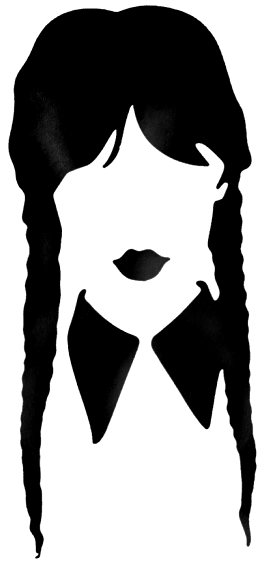
\includegraphics[height=1.35em]{figures/icons/mira-silhouette.png}}{}}}\enspace{\scshape\color{black}Scene}\enspace\textperiodcentered\enspace{\bfseries #1}\pdblockheadingend{\itshape #2}}%
    \end{tcolorbox}\par\addvspace{8pt plus 2pt}%
  }%
  \long\def\xrefbox#1{\par\pd@settle\addvspace{4pt}\noindent\pd@marginhead{See also}{\small #1}\par\addvspace{4pt}}%
  % A generic "Thesis" margin label does not identify which claim matters.
  % Keep the prose; use an authored keyidea head only when it adds meaning.
  \long\def\pdthesis#1{\par\pd@settle\addvspace{6pt plus 1pt}\noindent#1\par\addvspace{6pt plus 1pt}}%
  \long\def\pullquote#1{\pdthesis{#1}}%
}
\makeatother

% Shared visual language for the Book's figures -- version 2.
% Twin: book/figures/pd-figure-language.tex (byte-identical; edit both).
% The standard behind it, the migration from v1 and the QA loop live in
% skills/tikz-diagram-craft/ (SKILL.md, references/figure-standard.md).
%
% This file defines voices, hues, weights and marks -- not layouts.  Every
% figure still chooses a grammar from its reader question.
%
% ===========================================================================
% 1.  THE TYPE LADDER.  Three voices, one size, each tied to a role.
%       pd title   bold      panel titles, row and actor heads, column heads
%       pd label   upright   node text, state names, axis titles, tick words,
%                            relation words on an edge, badge numerals
%       pd note    italic    the one annotation a figure is allowed
%     `pd tag` is the label voice knocked out of the page, for a word that
%     must sit near a rule.  `pd kind` (small caps) is a one- or two-word kind
%     tag, never a title.  Every piece of figure text is mixed case; \texttt
%     only for identifiers that are literally code; math mode for symbols.
%
% 2.  THE COLOUR SYSTEM.  Hue is meaning, and the meanings cross chapters.
%     The figure's own subject is drawn in the CHAPTER hue (`pd focus ...`),
%     resolved from \pdcurrentchaptercolor, which the Book sets per chapter;
%     a fragment declares its standalone fallback with \pdfigurehue{...}.
%     Anything else the figure names takes its concept hue:
%       pd truth       pdcobalt   kernel, truth, the thing being specified
%       pd legible     pdteal     legibility, digest, inspection
%       pd ready       pdhealth   ready, coordinated, admitted, passing
%       pd protocol    pdindigo   protocol, federation, the wire
%       pd identity    pdviolet   identity, continuity, a card, an ID
%       pd reputation  pdrust     reputation, trust earned over time
%       pd value       pdgold     economy, value, settlement, payment
%       pd breach      pderror    breach, refusal, revocation, correction
%       pd warn        pdamber    warning; rules and stripes only, never text
%     Each concept X yields X, X rule, X arrow, X state, X fill, X datum and
%     X label.  Two to four hues a figure; colour is always doubled by shape,
%     dash, weight or a word (breach and warn are dashed as well as coloured).
%
% 3.  THE WEIGHT LADDER.  Exactly three weights, .5 / .9 / 1.6 pt
%     (1 : 1.8 : 3.2).  .5: hairline, guide, tick, artifact edge, fill edge,
%     mark outline, badge.  .9: rule, arrow, state edge, concept arrow.
%     1.6: spine, focus rule, focus and concept state edges, concept rule.
%     A reader sees which line is the subject.  Tips scale with the stroke.
%
% 4.  THE SURFACE LADDER.  pd state (page ground, ink edge) < pd artifact
%     (page ground, grey edge, subordinate) < pd focus state and the concept
%     states (24 % tint, edged in the same hue).  Text is always ink.  A
%     terminal state has a double boundary; an automaton's states are circles
%     (`pd automaton state/focus/terminal`); a ledger's pools are buckets
%     joined by pipes (`pd bucket`, `pd pipe`); a trust boundary is a dashed
%     rectangle (`pd trust boundary`).
%
% 5.  THE GROUND.  Body pages print on white, so every knockout and every
%     neutral surface is `pdpage` (white), never cream: a cream backing on a
%     white page reads as a sticker, which is what v1's figures were covered
%     in.  Neutral regions (Gantt bands, wells) are a warm grey tint.
%
% 6.  EDITIONS.  The Book sets \pdedition (maritime | swiss | technical) and
%     figures/pd-figure-language-<edition>.tex restyles the same names, so one
%     drawing renders in each edition's character.  A fragment that names a
%     raw colour (hhteal, pdcobalt!40, blue) bypasses this; name a role.
% ===========================================================================
% Libraries every v2 mark needs (diamonds, braces, markings), and
% pgfplots for computed plots. This file is \input in every preamble (the
% Book's and each standalone chapter's), so a plot works in all of them.
\usetikzlibrary{arrows.meta,matrix,patterns.meta,positioning,calc,fit,
  backgrounds,shapes.geometric,shapes.multipart,shapes.misc,decorations.pathreplacing,
  decorations.markings,quotes,intersections}
\RequirePackage{pgfplots}
\pgfplotsset{compat=1.18}
\usepgfplotslibrary{fillbetween,groupplots}

\colorlet{pdpage}{white}

% --- the chapter hue, resolved late --------------------------------------
% \pdfigurehue{pdindigo} on the line before a tikzpicture names the hue the
% figure is drawn in when it is compiled outside the Book (a standalone
% chapter, or the skill's renderer).  Inside the Book the preamble has already
% defined \pdcurrentchaptercolor and the chapter opener sets it, so there the
% opener wins and \providecommand does nothing.  Local to the figure's group.
\newcommand{\pdfigfraghue}{pdcobalt}
\newcommand{\pdfigurehue}[1]{%
  \renewcommand{\pdfigfraghue}{#1}%
  \providecommand{\pdcurrentchaptercolor}{#1}}
\newcommand{\pdsetfocushue}{%
  \ifdefined\pdcurrentchaptercolor
    \colorlet{pdfocus}{\pdcurrentchaptercolor}%
  \else
    \colorlet{pdfocus}{\pdfigfraghue}%
  \fi}
\colorlet{pdfocus}{pdcobalt}

% ===========================================================================
% THE TYPOGRAPHIC LAW
% ===========================================================================
% Companion to the line-weight law in figures/pd-palette.tex (1px texture,
% 1.5px linework, 2px enclosure). Same shape of rule: name the roles, fix the
% values, one place.
%
% ONE SIZE. Every named text role in a figure is \pdfiglabelsize
% (= \footnotesize). Roles separate by WEIGHT, SLOPE, FAMILY and INK -- never
% by size. A fragment never writes a size command of its own; if a distinction
% needs making, it takes the role that makes it.
%
% Where the size comes from. Measured, not chosen:
%   \tiny  \scriptsize  \footnotesize  \small  \normalsize
%   5.23    6.97          8.72           9.55    10.46  pt   Book (10.5pt
%                                                            Pagella, 4.5in
%                                                            column, 7x10in)
%   5.98    7.97          8.97           9.96    10.91  pt   standalone chapter
%                                                            (11pt Latin Modern)
% \scriptsize renders at 6.97pt in the Book -- under figcheck's 7pt T1 floor
% before a single width promotion, so it is illegal by measurement, not taste.
% \footnotesize holds 8.72pt and still clears the floor at the 0.85 \resizebox
% limit craft-rules sets (7.41pt). It is also what the corpus already voted
% for: 78 of the 91 local font= declarations this law replaces were already
% \footnotesize, \footnotesize\bfseries or \footnotesize\itshape.
%
% \pdfigbasesize (= \small) is the tikzpicture's ambient size only, so an
% unstyled node is never SMALLER than a styled one; every named role steps
% down exactly one notch from it and none steps down twice.
%
% ONE FACE, AND IT IS THE DOCUMENT'S. \pdfiglabelfamily is empty by default,
% which means figure type inherits whatever face the document is setting --
% Palatino in the Book, Computer Modern in a standalone chapter. Figures
% agreeing with EACH OTHER is not the goal; figures agreeing with the
% paragraph beside them is. A fragment therefore never names a family. Not
% \sffamily (which resolves to Latin Modern Sans against a Computer Modern
% page and reads as a foreign object on it), not \rmfamily, not
% \fontfamily{...}. P18 in tikz_precheck.py is an error for exactly that.
% An edition MAY substitute a face -- the Swiss and technical editions set
% \pdfiglabelfamily to \pdgrotesk, because grotesk display is their declared
% character -- and it does so in ONE command in ONE file, so the substitution
% is a decision on the record rather than an accident in a fragment. The
% only family a fragment may ask for is the identifier one, and it asks for
% it by role (pd mono label / \pdfiglabelmono), never by \ttfamily.
%
% What the roles are, and what each one is for:
%   pd panel title        bold        the name of a panel
%   pd row label          bold        an actor/row name east of its lane
%   pd reverse row label  bold, cream a row name sitting on a dark band
%   pd axis label         regular     an axis title or a tick numeral
%   pd direct label       regular     a value or name riding its own mark
%   pd reverse label      regular, cream  a direct label on a dark band
%   pd mono label         mono        an identifier, path, or literal
%   pd verdict            bold        a terminal outcome stamp (CLEAR, REJECT)
%   pd note               italic      one aside per figure
%   pd legend             regular     a pgfplots legend entry
%   pd state / terminal / actor / artifact / decision   node text
%   pd axis               the whole pgfplots typographic block, one key
%   \pdfigsub             a gloss line under a heading INSIDE a node
%   \pdfigmath            math carrying a sub/superscript, inside a label
%
% A fragment that needs a compound style of its own composes it from a role
% above (`gate/.style={pd decision,minimum width=2cm}`), or, where no role
% fits, from the \pdfiglabel* handles here. It never writes a raw size
% command: P16 in skills/harbor-chartwork/scripts/tikz_precheck.py is an
% error for exactly that, and P10/P11 have been errors for \tiny and
% \scriptsize since before this law.
%
% What does NOT transfer from the screen rules these roles otherwise follow.
% The dataviz method those rules come from assumes an interactive chart: a
% tooltip carries any value a label could not fit, a filter row rescopes the
% view, hover lifts the hovered mark. A printed page has none of that, and the
% absence is not a defect to design around. The INTENT of the tooltip rule --
% "every value is reachable without gating" -- does transfer, and on this page
% it is discharged somewhere else: the value is in the caption, in the margin
% apparatus, or in the chapter's own worked example. So a label that will not
% fit inside its mark moves outside the mark or is dropped to the caption; it
% is never shrunk to fit, because there is no size below \footnotesize to shrink
% to, and never clipped. Do not add a hover affordance, a legend toggle, or a
% filter to a figure in this book.
%
% IDENTIFIERS GET ONE SPELLING. A key, a cell id, a file name or any other
% literal a reader could type is set in `pd mono label` (or \pdfiglabelmono
% inside a compound style), spelled exactly as the code spells it: sk_A, not
% skA and not sk with a subscript A; card0, not card-nought and not a Unicode
% subscript zero. A figure that shows the same identifier two ways has told
% the reader they are two things. The subscripted form belongs to MATHEMATICS
% ($\kappa_7$, an index into a sequence) and the literal form to CODE -- one
% figure may use both, for different objects, but never both for the same
% one. (A precheck for two spellings of one identifier inside a fragment is
% being added on another branch; this is the convention it will enforce.)
%
% SHAPE IS A CHANNEL, AND IT HAS TO SURVIVE THE PRINT SIZE. pd datum, pd
% focus datum and pd caution datum carry three different forms, because the
% house palette is three low-chroma print inks and every distinction it makes
% has to be doubled by something that is not colour. That only counts if the
% form is still legible at 2.1-2.7 pt: an edition that flattens all three to
% one form has removed the second channel and left the figure separating its
% classes by hue alone, which fails in greyscale and for a colour-blind
% reader. Any edition override that restyles a datum must keep three
% distinguishable forms, and must be checked on a render at 1.0x, not
% reasoned about from the point sizes.
%
% One screen rule that does NOT bind here, and why. "Text never wears the data
% colour" exists because a light categorical hue is illegible as text on a
% light surface. The house figure hues are print inks, not screen hues --
% hhink #1B1712, hhteal #00564C, hhamber #6B4500 -- and all three clear text
% contrast on cream, so a label MAY wear its series' ink to bind itself to a
% curve, which is direct labelling and saves a legend. The rule that survives
% is the reason behind it: text wears one of those three inks at full
% strength, or hhink!80!hhgray for recessive furniture, and nothing else. A
% tint of an ink (text=hhgray, text=hhteal!60) is not a role; it is a fade.
% ===========================================================================

\providecommand{\pdfiglabelfamily}{}            % an edition may set \pdgrotesk
\providecommand{\pdfiglabelsize}{\footnotesize} % every named text role
\providecommand{\pdfigbasesize}{\small}         % the picture's ambient size
\providecommand{\pdfiglabel}{\pdfiglabelfamily\pdfiglabelsize}
\providecommand{\pdfiglabelbold}{\pdfiglabel\bfseries}
\providecommand{\pdfiglabelitalic}{\pdfiglabel\itshape}
\providecommand{\pdfiglabelmono}{\pdfiglabelsize\ttfamily}
% The one role that is not a node style, because it lives INSIDE a node's text:
% the second line under a heading that glosses it ("reviewer role / obligation +
% capability + authority"). Every fragment that needed it reached for \tiny or
% \scriptsize, which is how seven \tiny and twelve \scriptsize survived P10/P11
% as hard errors in the corpus. It steps down by SLOPE and WEIGHT, not size, so
% it stays legible and stays legal, and it touches neither family nor ink --
% which is what lets it sit on a reversed node without vanishing.
\providecommand{\pdfigsub}{\mdseries\itshape}
% The one place the law's own size is not the right size.
%
% Measured, both preambles, on a subscripted label inside `pd direct label`:
%
%              base glyph   subscript   subscript as % of base
%   chapter      8.97pt       5.98pt            66.7%
%   Book         8.72pt       6.36pt            72.9%
%   promoted    10.91/10.46   7.97/7.64
%
% An earlier version of this comment said those subscripts are "under figcheck's
% 7pt T1 floor". They are not, and the correction is worth more than the claim
% was. T1 has TWO bands: running text is held to 7.0pt, and a span of three
% glyphs or fewer -- a sub/superscript, a tick numeral -- is held to 5.9pt
% (T1_SHORT_SPAN_PT). That second band is not a loophole. A subscript is set at
% roughly 70% of its base by every typesetter that has ever existed; holding one
% to the running-text floor would mean either no subscripts in figures at all,
% or a figure whose base type is 10pt against 8.72pt body text.
%
% So \pdfigmath is NOT a T1 remedy, and using it as one is how a rule gets
% applied where it does not belong. It exists because 5.98pt clears the
% short-span band by 0.08pt, and 0.08pt is not a margin: a font substitution, an
% edition that nudges \pdfigbasesize, or a chapter that loads a different math
% font puts that subscript under the band with nobody having decided anything.
% Promotion puts it at 7.97/7.64pt -- over even the running-text floor -- while
% the base glyph stays close enough to its neighbours that the label still reads
% as one label.
%
% Use it ONLY for a math group that carries a sub- or superscript. Plain math
% takes the label's own size like any other text, and P22 in tikz_precheck.py is
% an error if it does not.
\providecommand{\pdfigmath}{\normalsize}

% ---------------------------------------------------------------------------
% THE GUIDE DASH, IN ABSOLUTE POINTS, IN ONE PLACE.
%
% `pd guide` used to read `line width=.45pt,densely dotted`. `densely dotted`
% expands to `dash pattern=on \pgflinewidth off 1pt`, and \pgflinewidth is read
% when the KEY is processed, not when the path is stroked. So the Swiss
% edition's `pd guide/.append style={draw=hhink!40,line width=.5pt}` widened the
% stroke and left the dash at the .45pt already baked into it. The canonical
% Book therefore shipped a 0.448pt dot on a 0.498pt stroke.
%
% MEASURED IN THE SHIPPED ARTIFACT, not in a probe: 50 guide strokes sampled
% pixel by pixel in the committed coordination-papers-mega-volume.pdf, at 150
% dpi / 1.0x.
%
%   on 0.448pt = 0.93 device px -- UNDER ONE PIXEL; off 0.996pt = 2.08 px
%   the dash DECLARES 69% of each line's length as gap
%   only 34% of each line's pixels actually reach paper
%   35.4% of three-period windows contain NO pixel that reaches paper at all
%
% That last number is the defect. The gap (2.08 px) is narrower than the
% antialias spread of a 0.93 px stroke, so as the pattern's phase drifts along a
% line the gaps fill in: over a third of every guide's length there is no gap
% left and it is a continuous grey stroke, while the rest of the same line still
% reads as dots. The ink arrives. The DOTTEDNESS does not. A reader sees one
% line that is dotted here and solid there, and no author chose that.
%
% Twenty-five of the corpus's thirty-six guide draws use dottedness to mean
% "this line is not a drawn edge", so twenty-five of them were making a
% distinction the page does not carry.
%
% After, same measurement, same probe geometry, Book preamble:
%   on 1.2pt = 2.50 px, off 2.0pt = 4.17 px, stroke .7pt = 1.45 px
%   0.0% of three-period windows are without paper -- every gap survives,
%     at every phase
%   50% of pixels reach paper against 62.5% declared, the shortfall now being
%     the stroke's antialias skirt rather than the whole signal
%
% ON THE INK, because the obvious reading of this change is wrong. The BASE pair
% was never the problem: hhgray!62 against the hairline's hhgray!78 is 0.411
% against 0.517 of nominal ink, well apart. The problem is that the Book renders
% the SWISS edition (\pdedition defaults to swiss; the committed Book PDF is
% full of hhink!40 guides), where the pair was hhink!40 against hhink!45 -- 4.6%
% of the grey scale. Deleting the Swiss override, which is the right fix for the
% geometry, makes the base ink govern the Book too -- and hhgray!62 is 0.411
% against the Book hairline's 0.410. The same grey, to a thousandth. So the base
% ink has to move, or the dash would go back to carrying the whole distinction
% by itself, which is how this started.
%
% hhink!70 measured against the hairline, mean ink on the page at 150 dpi:
%   chapter  guide 0.0502  hairline 0.0790   guide is 64% of the hairline
%   Book     guide 0.0545  hairline 0.0671   guide is 81% of the hairline
% Per DOT it is 0.638 against 0.410 -- unmistakably a different mark. In MEAN it
% is still lighter than the hairline -- so it still recedes. Two channels, both
% working, instead of one that does not.
%
% The replacement is stated absolutely and measures phase-STABLE: every dot
% renders at the same weight wherever it falls on the grid (peak column ink
% 0.808, invariant across twelve sub-pixel offsets). It is a macro rather than
% three numbers because an edition that restates one of them and not the others
% is how this defect happened. The geometry is a LEGIBILITY FLOOR, not an
% edition's character: an edition may move the guide's ink, and states the
% geometry through these two macros so it cannot half-restate it.
%
% Any dash in this corpus is stated in absolute points. The `dotted` family
% (`dotted`, `densely dotted`, `loosely dotted`) derives its on-length from the
% line width and is therefore banned -- P23 in tikz_precheck.py. `dashed` and
% its relatives are absolute (on 3pt off 3pt) and are fine.
\providecommand{\pdguidewidth}{.7pt}
% Three lengths, not one macro holding the whole key: pgfkeys splits a key list
% on `,` and `=` before expanding anything (so a macro carrying `dash
% pattern=...` is read as one key NAME), and TikZ's dash-pattern scanner reads
% the literal words `on`/`off` without expanding a macro that hides them. A
% dimension after each word does expand, which is the seam that works.
\providecommand{\pdguideon}{1.2pt}
\providecommand{\pdguideoff}{2.0pt}

\tikzset{
  % --- picture level: one size, one default tip, the chapter hue -----------
  % A figure label is a name, not prose: it never hyphenates.
  pd figure/.style={font=\pdfiglabelfamily\pdfigbasesize,text=pdink,line cap=round,line join=round,
    >={Stealth[length=2.6pt 3.2,width=2.0pt 2.4]},/utils/exec=\pdsetfocushue,
    every node/.append style={execute at begin node={%
      \hyphenpenalty=10000\exhyphenpenalty=10000\relax}}},
%
  % --- 1. the voices ---------------------------------------------------------
  pd title/.style={font=\pdfiglabelbold,text=pdink,align=center},
  pd label/.style={font=\pdfiglabel,text=pdink,align=center},
  pd note/.style={font=\pdfiglabelitalic,text=pdinkmuted,align=left},
  pd kind/.style={font=\pdfiglabel\scshape,text=pdinkmuted,align=center},
  pd tag/.style={pd label,fill=pdpage,inner sep=1.7pt},
%
  % --- 4. surfaces -----------------------------------------------------------
  pd state/.style={pd label,draw=pdink,line width=.9pt,fill=pdpage,
    rounded corners=1pt,inner xsep=6pt,inner ysep=4.5pt,minimum height=7.4mm},
  % a terminal state carries a double boundary, as every automaton text draws it
  pd terminal/.style={pd state,double=pdpage,double distance=1.1pt,line width=.5pt},
  pd artifact/.style={pd label,draw=pdinkmuted!60,line width=.5pt,fill=pdpage,
    rounded corners=1pt,inner xsep=5pt,inner ysep=3.5pt,minimum height=6.2mm},
  pd panel/.style={draw=pdinkmuted!55,line width=.5pt,
    dash pattern=on 2.4pt off 2pt,rounded corners=2.5pt,inner sep=7pt,align=center},
  pd hatch/.style={pattern={Lines[angle=45,distance=4pt,line width=.3pt]},
    pattern color=pdinkmuted!70},
  pd neutral fill/.style={fill=pdinkmuted!12,draw=pdinkmuted!55,line width=.5pt},
%
  % --- 3. strokes ------------------------------------------------------------
  pd hairline/.style={draw=pdinkmuted!45,line width=.5pt},
  % Absolute dash, from the typographic law's three macros above: a guide is a
  % definite dotted construction line, darker per dot than the hairline and
  % lighter in mean ink. A lattice is the quiet continuous grid a figure stands on.
  pd guide/.style={draw=pdink!70,line width=\pdguidewidth,dash pattern=on \pdguideon off \pdguideoff},
  pd lattice/.style={draw=pdinkmuted!40,line width=.4pt},
  pd tick/.style={draw=pdinkmuted!75,line width=.5pt},
  pd rule/.style={draw=pdink,line width=.9pt},
  pd spine/.style={draw=pdink,line width=1.6pt},
  pd thin arrow/.style={draw=pdinkmuted!75,line width=.5pt,->},
  pd arrow/.style={pd rule,->},
  pd spine arrow/.style={pd spine,->},
%
  % --- the chapter hue, as the figure's focus --------------------------------
  pd focus rule/.style={draw=pdfocus,line width=1.6pt},
  pd focus arrow/.style={pd focus rule,->},
  pd focus state/.style={pd state,draw=pdfocus,line width=1.6pt,fill=pdfocus!24},
  % The single solid chapter-colour surface in a figure: use only for the
  % culmination or object the reader should name after five seconds. Editions
  % may render ordinary focus with a pale field while keeping this one solid.
  pd climax state/.style={pd focus state},
  % a member of the subject's set when the set, not one node, is the subject:
  % edged in the chapter hue, never filled, so the one solid node stays unique
  pd focus outline/.style={pd state,draw=pdfocus,line width=1.2pt,fill=pdpage},
  pd focus fill/.style={fill=pdfocus!24,draw=pdfocus,line width=.5pt},
  pd focus datum/.style={circle,fill=pdfocus,draw=pdpage,line width=.5pt,inner sep=2.6pt},
  pd focus label/.style={pd label,text=pdfocus!85!pdink},
%
  % --- marks -----------------------------------------------------------------
  pd datum/.style={circle,fill=pdink,draw=pdpage,line width=.5pt,inner sep=2.3pt},
  pd badge/.style={pd label,circle,draw=pdink,line width=.5pt,fill=pdpage,
    inner sep=.5pt,minimum size=5.0mm},
  pd focus badge/.style={pd badge,draw=pdfocus,line width=.9pt,fill=pdfocus!24},
  % --- conventions shared by every chapter (Critical Analysis, 2026-09-08) ---
  % Automata: states are circles, terminal (accepting) states double circles;
  % edge words are short action names; guards go in an aligned legend table.
  pd automaton state/.style={pd label,circle,draw=pdink,line width=.9pt,fill=pdpage,
    minimum size=11mm,inner sep=1pt},
  pd automaton focus/.style={pd automaton state,draw=pdfocus,line width=1.6pt,fill=pdfocus!24},
  pd automaton terminal/.style={pd automaton state,double=pdpage,double distance=1.1pt,
    line width=.5pt},
  pd initial/.style={draw=pdink,line width=.9pt,->},
  % Ledgers: asset pools are rectangular buckets (open at the top) joined by
  % directed pipes; the conserved sum is set as an equation under the rails.
  pd bucket/.style={pd label,draw=none,minimum width=2.2cm,minimum height=1.3cm,
    append after command={\pgfextra{\draw[draw=pdink,line width=.9pt]
      (\tikzlastnode.north west) -- (\tikzlastnode.south west)
      -- (\tikzlastnode.south east) -- (\tikzlastnode.north east);}}},
  pd pipe/.style={draw=pdink,line width=.9pt,double=pdpage,double distance=2.2pt,
    -{Stealth[length=3.4pt 2,width=5.2pt]}},
  pd focus pipe/.style={pd pipe,draw=pdfocus},
  % Trust boundaries: a dashed rectangle is the Dolev-Yao interface; a vector
  % that escapes it is drawn in pd breach and named.
  pd trust boundary/.style={draw=pdink,line width=.9pt,dash pattern=on 4pt off 2.4pt,
    rounded corners=0pt,inner sep=8pt},
  % a stroke that ends at a badge is shortened, so no rule touches the numeral
  pd to badge/.style={shorten >=2pt},
  pd from badge/.style={shorten <=2pt},
}

% ===========================================================================
% 7.  PLOTS.  A plot is computed by a committed script, never sketched.  `pd
%     axis` is the one axis grammar: two spines (left, bottom), ticks out, no
%     box, no grid unless asked (`pd grid`), tick words in the label voice,
%     numbers with a thin-space thousands separator, room outside the plot for
%     direct labels (clip=false).  Series are named at their ends, not in a
%     legend: `pd series` (ink), `pd focus series` (chapter hue), and
%     `pd X series` for a concept; breach and warn series are dashed.  A
%     region between curves is `pd focus fill`/`X fill` with fillbetween.
%     Width: `width=` is the plot box (scale only axis); leave about 1.6 cm
%     of the 11.4 cm column for the y tick words and title.
% ===========================================================================
\pgfplotsset{
  pd axis/.style={
    scale only axis,width=8.8cm,height=4.6cm,
    axis lines*=left,axis line style={draw=pdink,line width=.5pt,-},
    tick align=outside,major tick length=3pt,minor tick length=0pt,
    tick style={draw=pdink,line width=.5pt},
    tick label style={pd label,text=pdinkmuted},
    label style={pd label},title style={pd title},
    every axis title/.append style={yshift=-2pt},
    enlargelimits=false,clip=false,
    grid=none,
    legend style={draw=none,fill=none,font=\pdfiglabel},
    /pgf/number format/1000 sep={\,},
    every axis plot/.append style={line width=.9pt,line join=round,mark size=1.7pt},
  },
  pd grid/.style={ymajorgrids,major grid style={draw=pdinkmuted!30,line width=.4pt}},
  pd series/.style={draw=pdink,mark=*,mark options={fill=pdink,draw=pdpage,line width=.5pt,solid}},
  pd focus series/.style={draw=pdfocus,line width=1.6pt,mark=*,
    mark options={fill=pdfocus,draw=pdpage,line width=.5pt,solid}},
  pd muted series/.style={draw=pdinkmuted!70,line width=.9pt,mark=none},
}
\newcommand{\pdplotconcept}[2]{%
  \pgfplotsset{#1 series/.style={draw=#2,mark=*,
    mark options={fill=#2,draw=pdpage,line width=.5pt,solid}}}}
\pdplotconcept{pd truth}{pdcobalt}
\pdplotconcept{pd legible}{pdteal}
\pdplotconcept{pd ready}{pdhealth}
\pdplotconcept{pd protocol}{pdindigo}
\pdplotconcept{pd identity}{pdviolet}
\pdplotconcept{pd reputation}{pdrust}
\pdplotconcept{pd value}{pdgold}
\pgfplotsset{
  pd breach series/.style={draw=pderror,dash pattern=on 3.2pt off 2.2pt,mark=diamond*,
    mark options={fill=pderror,draw=pdpage,line width=.5pt,solid}},
  pd warn series/.style={draw=pdamber,dash pattern=on 3.2pt off 2.2pt,mark=none},
}

% ===========================================================================
% Supplied visual-guide primitives: native Book type, deliberate strokes,
% readable Stealth heads, open markers, and a quiet quantitative grid.
% These are opt-in: old diagrams need spacing review before thicker arrows.
\tikzset{
  pd guide step/.style={pd artifact,draw=pdink,fill=pdpage,line width=1pt,
    align=center,minimum height=40pt,inner xsep=5pt,inner ysep=6pt},
  pd guide arrow/.style={draw=pdcobalt,line width=1.15pt,
    -{Stealth[length=7pt,width=4.4pt]},shorten <=2pt,shorten >=2pt},
}
\newcommand{\pdflowstep}[4]{%
  \node[pd guide step,text width=#4] (#1) at #2 {#3};}
\newcommand{\pdflowlink}[2]{%
  \draw[pd guide arrow] (#1.east)--(#2.west);}
\pgfplotsset{
  pd evidence axis/.style={pd axis,
    axis line style={draw=pdink,line width=1pt,-},
    tick style={draw=pdink,line width=.8pt},
    grid=major,major grid style={draw=pdinkmuted!20,line width=.35pt},
    axis background/.style={fill=pdpage}},
  pd evidence measured/.style={draw=pdcobalt,line width=1.35pt,mark=*,
    mark size=2.6pt,mark options={fill=pdpage,draw=pdcobalt,line width=1.1pt}},
  pd evidence comparison/.style={draw=pdink,line width=1.1pt,
    dash pattern=on 4pt off 2.5pt,mark=square*,mark size=2.2pt,
    mark options={fill=pdink,draw=pdink,solid}},
}
% Analytic curves, not sampled observations. Integer samples preserve the
% meaning of reviewer count; callers set axes and name their assumptions.
\newcommand{\pdindependentmisses}[2]{%
  \addplot[pd evidence measured,domain=1:#2,samples=#2] {100*(1-#1)^x};}
\newcommand{\pdreviewcost}[1]{%
  \addplot[pd evidence measured,domain=1:#1,samples=#1] {x};}
% 8.  UML.  The Book's engineering diagrams use UML 2.5 notation, so a reader
%     who knows UML reads them without a key.  Four kinds:
%     STATE MACHINE  `pd uml state` (rounded), `pd uml focus state`, a
%       composite drawn with `pd uml composite` around its substates plus a
%       compartment of internal transitions; `pd uml initial` (filled dot),
%       `pd uml final` (bullseye), `pd uml choice` (diamond); transitions are
%       `pd uml transition` (open arrowhead) labelled  event [guard] / effect.
%     SEQUENCE  `pd uml head` (lifeline head), `pd uml lifeline` (dashed),
%       `pd uml activation` (thin bar), messages `pd uml sync` (filled head),
%       `pd uml async` (open head), `pd uml reply` (dashed, open head),
%       `pd uml fragment` + `pd uml fragment tag` for alt / opt / loop.
%     COMPONENT  `pd uml component` with \pdumlicon{node} (the component
%       glyph) and a <<component>> keyword; `pd uml port`; provided interface
%       \pdumlprovided{from}{to}{name} (lollipop), required \pdumlrequired (socket).
%     ERD (crow's foot)  `pd er entity` (rectangle split: name, then rows;
%       mark keys PK / FK in the row text), relationship lines `pd er rel`
%       with tips `er one`, `er many`, `er zero or one`, `er one or many`,
%       `er zero or many` at either end.
% ===========================================================================
\pgfdeclarearrow{
  name = pd crow,
  parameters = {\the\pgfarrowlength,\the\pgfarrowwidth},
  setup code = {%
    \pgfarrowssettipend{0pt}%
    \pgfarrowssetlineend{0pt}%
    \pgfarrowssetbackend{-\pgfarrowlength}%
    \pgfarrowsupperhullpoint{0pt}{.5\pgfarrowwidth}%
    \pgfarrowsupperhullpoint{-\pgfarrowlength}{0pt}%
    \pgfarrowssavethe\pgfarrowlength
    \pgfarrowssavethe\pgfarrowwidth},
  drawing code = {%
    \pgfsetdash{}{0pt}%
    \pgfpathmoveto{\pgfqpoint{-\pgfarrowlength}{0pt}}%
    \pgfpathlineto{\pgfqpoint{0pt}{.5\pgfarrowwidth}}%
    \pgfpathmoveto{\pgfqpoint{-\pgfarrowlength}{0pt}}%
    \pgfpathlineto{\pgfqpoint{0pt}{-.5\pgfarrowwidth}}%
    \pgfusepathqstroke},
  defaults = {length=2.4mm, width=3.0mm}
}
\tikzset{
  % state machine
  pd uml state/.style={pd state,rounded corners=4.5pt},
  pd uml focus state/.style={pd focus state,rounded corners=4.5pt},
  pd uml terminal/.style={pd terminal,rounded corners=4.5pt},
  pd uml composite/.style={draw=pdink,line width=.9pt,rounded corners=7pt,fill=none,inner sep=0pt},
  pd uml initial/.style={circle,fill=pdink,draw=none,minimum size=2.4mm,inner sep=0pt},
  pd uml final/.style={circle,draw=pdink,line width=.9pt,fill=pdpage,minimum size=3.6mm,inner sep=0pt,
    path picture={\fill[pdink] (path picture bounding box.center) circle (1.1mm);}},
  pd uml choice/.style={diamond,draw=pdink,line width=.9pt,fill=pdpage,minimum size=4.2mm,inner sep=0pt},
  pd uml transition/.style={pd rule,-{Straight Barb[length=2.2pt 2.2,width=4.4pt 2.2]}},
  pd uml focus transition/.style={pd focus rule,-{Straight Barb[length=2.2pt 2.2,width=4.4pt 2.2]}},
  pd uml breach transition/.style={pd rule,draw=pderror,dash pattern=on 3.2pt off 2.2pt,
    -{Straight Barb[length=2.2pt 2.2,width=4.4pt 2.2]}},
  % sequence
  pd uml head/.style={pd state,rounded corners=0pt,minimum height=6.8mm},
  pd uml lifeline/.style={draw=pdinkmuted!75,line width=.5pt,dash pattern=on 3pt off 2pt},
  pd uml activation/.style={draw=pdink,line width=.5pt,fill=pdpage,minimum width=2.2mm,inner sep=0pt},
  pd uml sync/.style={pd rule,-{Triangle[length=3.2pt 1.6,width=3.2pt 1.6]}},
  pd uml async/.style={pd rule,-{Straight Barb[length=2.4pt 2,width=4.4pt 2]}},
  pd uml reply/.style={pd rule,dash pattern=on 3pt off 2pt,-{Straight Barb[length=2.4pt 2,width=4.4pt 2]}},
  pd uml fragment/.style={draw=pdink,line width=.5pt,fill=none,inner sep=6pt},
  pd uml fragment tag/.style={pd label,font=\footnotesize\bfseries,draw=pdink,line width=.5pt,fill=pdpage,
    inner xsep=3pt,inner ysep=2pt,chamfered rectangle,chamfered rectangle corners=south east,
    chamfered rectangle xsep=2pt},
  % component
  pd uml component/.style={pd state,rounded corners=0pt,align=center,inner xsep=8pt,inner ysep=6pt,minimum height=11mm},
  pd uml port/.style={rectangle,draw=pdink,line width=.5pt,fill=pdpage,minimum size=2mm,inner sep=0pt},
  % ERD
  pd er entity/.style={pd label,rectangle split,rectangle split parts=2,rectangle split part align={center,left},
    draw=pdink,line width=.9pt,fill=pdpage,inner xsep=5pt,inner ysep=3pt,align=left,
    rectangle split part fill={pdinkmuted!12,pdpage}},
  pd er rel/.style={pd rule},
  er one/.tip={Bar[width=3.0mm,sep=1.2pt]Bar[width=3.0mm]},
  er many/.tip={Bar[width=3.0mm,sep=1.4pt]pd crow},
  er zero or one/.tip={Circle[open,length=1.8mm,width=1.8mm,sep=1.2pt,fill=pdpage]Bar[width=3.0mm]},
  er one or many/.tip={Bar[width=3.0mm,sep=1.4pt]pd crow},
  er zero or many/.tip={Circle[open,length=1.8mm,width=1.8mm,sep=1.2pt,fill=pdpage]pd crow},
}
% the component glyph, drawn in the top-right corner of a component node
\newcommand{\pdumlicon}[1]{%
  \begin{scope}[shift={($(#1.north east)+(-4.2mm,-2.6mm)$)},x=1mm,y=1mm]
    \draw[pdink,line width=.5pt,fill=pdpage] (0,-1.1) rectangle (2.6,1.1);
    \draw[pdink,line width=.5pt,fill=pdpage] (-.6,.25) rectangle (.6,.65);
    \draw[pdink,line width=.5pt,fill=pdpage] (-.6,-.65) rectangle (.6,-.25);
  \end{scope}}
% a provided interface (lollipop) from a node side to a point, with its name
\newcommand{\pdumlprovided}[3]{%
  \draw[pd rule] (#1) -- (#2);
  \draw[pd rule,fill=pdpage] (#2) circle (1.3mm);
  \node[pd label,anchor=south] at ($(#2)+(0,1.6mm)$) {#3};}
% a required interface (socket): a half-circle open toward the provider
\newcommand{\pdumlrequired}[4]{% from, to, name, facing angle of the socket's opening
  \draw[pd rule] (#1) -- (#2);
  \draw[pd rule] ($(#2)+(#4+90:1.9mm)$) arc[start angle=#4+90,end angle=#4+270,radius=1.9mm];
  \node[pd label,anchor=north] at ($(#2)+(0,-2.4mm)$) {#3};}

% --- 2. the concept map, as styles, so a drawing never chooses a hue --------
% An edition file may \renewcommand\pdconcept before the map below expands.
\newcommand{\pdconcept}[2]{%
  \tikzset{%
    #1/.style={draw=#2,text=pdink},
    #1 rule/.style={draw=#2,line width=1.6pt},
    #1 arrow/.style={draw=#2,line width=.9pt,->},
    #1 state/.style={pd state,draw=#2,line width=1.6pt,fill=#2!24},
    #1 fill/.style={fill=#2!24,draw=#2,line width=.5pt},
    #1 datum/.style={circle,fill=#2,draw=pdpage,line width=.5pt,inner sep=2.6pt},
    #1 label/.style={pd label,text=#2!85!pdink},
  }}

% --- 6. the edition layer, loaded before the concept map expands ----------
\ifdefined\pdedition\IfFileExists{figures/pd-figure-language-\pdedition.tex}{\input{figures/pd-figure-language-\pdedition}}{}\fi

\pdconcept{pd truth}{pdcobalt}
\pdconcept{pd legible}{pdteal}
\pdconcept{pd ready}{pdhealth}
\pdconcept{pd protocol}{pdindigo}
\pdconcept{pd identity}{pdviolet}
\pdconcept{pd reputation}{pdrust}
\pdconcept{pd value}{pdgold}
\pdconcept{pd breach}{pderror}
\pdconcept{pd warn}{pdamber}
% Breach and warning read as refusals, so they are dashed as well as
% coloured, and a breach mark is a diamond where every other mark is a circle.
% Amber is never text (3.71:1 on white); a warn label is set in ink.
\tikzset{
  pd breach rule/.append style={dash pattern=on 3.2pt off 2.2pt},
  pd breach arrow/.append style={dash pattern=on 3.2pt off 2.2pt},
  pd warn rule/.append style={dash pattern=on 3.2pt off 2.2pt},
  pd warn arrow/.append style={dash pattern=on 3.2pt off 2.2pt},
  pd breach datum/.append style={diamond},
  pd warn label/.style={pd label},
}

% ===========================================================================
% v1 NAMES.  Kept so every existing fragment still compiles; they resolve to
% the v2 roles, so an untouched figure inherits the ladder.  New work uses the
% v2 names (skills/tikz-diagram-craft/references/migration-v1-to-v2.md).
% ===========================================================================
\tikzset{
  pd row label/.style={pd title,anchor=east},
  pd panel title/.style={pd title,align=left},
  pd axis label/.style={pd label},
  % Direct labels sit beside their mark; they do not erase a line or box
  % underneath themselves. A label that needs a paper knockout is misplaced
  % and must be moved, not given an invisible patch.
  pd direct label/.style={pd tag,fill=none,align=left},
  pd actor/.style={pd state},
  pd boundary/.style={pd panel},
  pd caution rule/.style={pd breach rule},
  pd caution arrow/.style={pd breach arrow},
  pd caution fill/.style={pd breach fill},
  pd caution datum/.style={pd breach datum},
}

% ===========================================================================
% Roles named on main by the typographic law (#10191), expressed on the v2
% roles so an edition's .append style on the parent reaches them. `pd danger`
% is main's name for what v2 calls `pd breach` (red, dashed, diamond marks);
% both names resolve to one family. Main's hairline-boxed fact badge is
% `pd fact badge`: v2's `pd badge` is the numbered guard/step marker.
% ===========================================================================
\tikzset{
  pd danger rule/.style={pd breach rule},
  pd danger arrow/.style={pd breach arrow},
  pd danger fill/.style={pd breach fill,text=pdink},
  pd danger datum/.style={pd breach datum},
  pd ink fill/.style={fill=pdink,draw=pdink,line width=.4pt,text=pdpage},
  pd decision/.style={pd state,diamond,aspect=1.55,font=\pdfiglabelbold,
    minimum height=0pt,inner xsep=3pt,inner ysep=3pt},
  pd mono label/.style={pd direct label,font=\pdfiglabelmono,inner xsep=2.5pt,inner ysep=2.5pt},
  pd verdict/.style={pd direct label,font=\pdfiglabelbold},
  pd reverse label/.style={pd direct label,text=pdpage,fill=none},
  pd reverse row label/.style={pd row label,text=pdpage},
  pd legend/.style={font=\pdfiglabel,text=pdink,draw=none,fill=none},
  pd kind tag/.style={pd kind,align=right},
  pd fact badge/.style={pd hairline,font=\pdfiglabel,text=pdink,align=center,
    inner sep=2.4pt,fill=none},
}

% Small reusable marks.  They deliberately avoid prose-bearing boxes.
\newcommand{\pdfigaxis}[4]{%
  \draw[pd rule,->] (#1,#2) -- (#3,#2);
  \node[pd label,anchor=west] at (#3,#2) {#4};
}
\newcommand{\pdfigvaxis}[4]{%
  \draw[pd rule,->] (#1,#2) -- (#1,#3);
  \node[pd label,anchor=south] at (#1,#3) {#4};
}

% Native-size, object-based evidence figures; shared by Book and chapters.
% Shared approved Swiss evidence drawing primitives. Keep both chapter roots identical.
\ifdefined\pdSwissEvidenceLoaded\else
\def\pdSwissEvidenceLoaded{1}
% Real ink-box gate; no declared coordinate envelope can substitute for this.
\newsavebox{\sgEvidenceBox}
\newcommand{\SGMeasuredFigure}[2]{%
  \sbox{\sgEvidenceBox}{#2}%
  \typeout{SG-GEOMETRY: #1,width=\the\wd\sgEvidenceBox,height=\the\dimexpr\ht\sgEvidenceBox+\dp\sgEvidenceBox\relax}%
  \ifdim\wd\sgEvidenceBox>325.215pt
    \PackageError{swiss-evidence}{Figure #1 exceeds the Book column}{Recompose at native text size; do not scale.}%
  \fi
  \usebox{\sgEvidenceBox}}
% Parent redraws after rejection of lab specimens 01,04,06.
% All coordinates are physical TeX points; no resizebox or transformed fonts.
\usetikzlibrary{arrows.meta,calc}
% Aliased onto the house palette (figures/pd-palette.tex), not \definecolor'd
% as independent HTML values: an edition that restyles pdcobalt/pdteal/...
% now restyles every SG figure with it. The six values were already
% bit-identical matches for pdcobalt/pdteal/pdviolet/pdamber/pderror/pdink;
% the alias turns that into a guarantee instead of a coincidence.
\colorlet{sgBlue}{pdcobalt}
\colorlet{sgTeal}{pdteal}
\colorlet{sgViolet}{pdviolet}
\colorlet{sgAmber}{pdamber}
\colorlet{sgRed}{pderror}
\colorlet{sgInk}{pdink}
\definecolor{sgGrid}{HTML}{D8C7A6}
% The one house size, inheriting the document's own face (the typographic
% law in pd-figure-language.tex): no \sffamily leak, no local \fontsize.
\newcommand{\SGType}{\pdfiglabel}
\tikzset{sg/base/.style={x=1pt,y=1pt,line cap=butt,line join=miter,
  every node/.style={font=\SGType,inner sep=0pt,text=sgInk}},
  sg/arrow/.style={-{Stealth[length=4.5pt,width=3.6pt]},draw=sgInk,line width=.85pt},
  sg/grid/.style={draw=sgGrid,line width=.3pt},
  sg/hash/.style={draw=sgBlue,fill=sgBlue!7,line width=1pt,minimum width=53pt,
    minimum height=27pt,inner sep=4pt,align=center},
  sg/sibling/.style={draw=sgAmber,fill=sgAmber!10,line width=1pt,minimum width=51pt,
    minimum height=27pt,inner sep=4pt,align=center},
  sg/check/.style={draw=sgInk,fill=white,line width=1pt,minimum width=92pt,
    minimum height=30pt,inner sep=5pt,align=center}}

% A folded record, not an undifferentiated rounded node. Width/height are pt.
\newcommand{\SGDocument}[6]{%
  \begin{scope}[shift={#2}]
    \path[draw=sgInk,fill=#5,line width=.85pt]
      (0,0)--({#3-7},0)--(#3,7)--(#3,#4)--(0,#4)--cycle;
    \draw[sgInk,line width=.65pt] ({#3-7},0)--({#3-7},7)--(#3,7);
    \node[minimum width=#3pt,minimum height=#4pt,text width=\dimexpr#3pt-12pt\relax,
      align=center] (#1) at ({#3/2},{#4/2}) {#6};
  \end{scope}}

\newcommand{\SGSurvival}{%
\begin{tikzpicture}[sg/base]
  % Three complete probability decades, percentages rather than tiny exponents.
  \foreach \x in {0,1,...,6}{\draw[sg/grid] ({35+30*\x},20)--({35+30*\x},140);}
  \foreach \y/\lab in {20/{0.1\%},60/{1\%},100/{10\%},140/{100\%}}{%
    \draw[sg/grid] (35,\y)--(215,\y);
    \draw[sgInk,line width=.65pt] (32,\y)--(35,\y);
    \node[anchor=east] at (28,\y) {\lab};}
  \draw[sgInk,line width=.85pt] (35,140)--(35,20)--(215,20);
  \foreach \x in {0,2,4,6}{%
    \draw[sgInk,line width=.65pt] ({35+30*\x},20)--({35+30*\x},17);
    \node[anchor=north] at ({35+30*\x},12) {$\x$};}
  \node[rotate=90] at (-9,80) {jobs still running (log scale)};
  \node[anchor=north] at (125,-5) {duration / mean duration};
  \draw[sgBlue,line width=1.5pt,domain=0:6,samples=100]
    plot ({35+30*\x},{140-120*ln(1+\x/2)/ln(10)});
  \draw[sgViolet,line width=1.2pt,dash pattern=on 4pt off 2.5pt,domain=0:6,samples=100]
    plot ({35+30*\x},{140-40*\x/ln(10)});
  % Endpoint leaders have allocated space; text does not lie on a curve.
  \draw[sgBlue,line width=.8pt] (215,67.75)--(224,67.75);
  \node[anchor=west,text=sgBlue,font=\SGType\bfseries] at (230,73) {Lomax};
  \node[anchor=west,text=sgBlue] at (230,60) {1.56\%};
  \draw[sgViolet,line width=.8pt,dashed] (215,35.77)--(224,35.77);
  \node[anchor=west,text=sgViolet,font=\SGType\bfseries] at (230,40) {exponential};
  \node[anchor=west,text=sgViolet] at (230,27) {0.248\%};
\end{tikzpicture}}

\newcommand{\SGTiming}{%
\begin{tikzpicture}[sg/base,y=-1pt]
  % This bracket spans COMMIT TO SYNC. It is not a range of hypothetical syncs.
  \path[draw=sgAmber!35,fill=sgAmber!9,line width=.5pt] (39,19) rectangle (253,49);
  \draw[sgAmber,line width=1pt] (39,18)--(39,9)--(253,9)--(253,18);
  \node[anchor=south,text=sgAmber,font=\SGType\bfseries] at (146,5) {?};
  \draw[sgInk,line width=.9pt] (39,27)--(39,45) (253,27)--(253,45);
  \draw[{Stealth[length=4.5pt,width=3.6pt]}-{Stealth[length=4.5pt,width=3.6pt]},
    sgAmber,line width=1.3pt] (40,36)--(252,36);
  \node[anchor=north,font=\SGType\bfseries] at (39,52) {commit};
  \node[anchor=north,font=\SGType\bfseries] at (253,52) {WAL sync};
  \node[anchor=west] at (0,86) {heartbeats received};
  \foreach \x/\label in {57/{s_1},117/{s_2},194/{s_3},278/{s_4}}{%
    \draw[sgViolet!70,dashed,line width=.55pt] (\x,104)--(\x,145);
    \node[anchor=south,text=sgViolet] at (\x,101) {$\label$};}
  \path[draw=sgAmber!35,fill=sgAmber!9,line width=.5pt] (158,108) rectangle (243,142);
  \draw[sg/grid] (0,139)--(306,139);
  \draw[sgTeal,line width=1.4pt]
    (0,132)--(25,132)--(25,116)--(33,116)--(33,132)
    --(85,132)--(85,116)--(93,116)--(93,132)
    --(145,132)--(145,116)--(153,116)--(153,132)--(306,132);
  \draw[sgRed,line width=1pt] (243,106)--(243,145);
  \node[anchor=north,text=sgRed] at (243,149) {deadline};
  \draw[sg/arrow] (0,174)--(306,174);
  \node[anchor=north east] at (306,179) {time};
\end{tikzpicture}}

\newcommand{\SGInclusion}{%
\begin{tikzpicture}[sg/base,y=-1pt]
  % Two independent inputs: a supplied proof and an issuer-authenticated root.
  \node[anchor=north west,font=\SGType\bfseries,text width=158pt,align=left] at (0,0)
    {Recompute from the receipt};
  \node[anchor=north west,font=\SGType\bfseries,text width=118pt,align=left] at (193,0)
    {Authenticate\\the checkpoint};
  \draw[sg/grid,step=15pt] (0,29) grid (175,194);
  \SGDocument{receipt}{(4,35)}{49}{34}{sgViolet!9}{receipt $P$}
  \node[sg/hash] (leaf) at (29,103) {$a=H_L(P)$};
  \node[sg/sibling] (sibone) at (108,103) {sibling $b$};
  \node[sg/hash] (inner) at (68,146) {$u=H_N(a,b)$};
  \node[sg/sibling] (sibtwo) at (146,146) {subtree $c$};
  \node[sg/hash,fill=sgBlue,text=white,minimum width=100pt] (computed) at (107,190)
    {$R'=H_N(u,c)$};
  \draw[sg/arrow,draw=sgViolet] (receipt.south)--(leaf.north);
  \draw[sg/arrow,draw=sgBlue] (leaf.south)--(inner.north west);
  \draw[sg/arrow,draw=sgAmber] (sibone.south)--(inner.north east);
  \draw[sg/arrow,draw=sgBlue] (inner.south)--(computed.north west);
  \draw[sg/arrow,draw=sgAmber] (sibtwo.south)--(computed.north east);
  \SGDocument{checkpoint}{(211,37)}{85}{48}{sgTeal!8}{signed root $R^*$\\size $n=4$\\signature $\sigma$}
  % The trusted key is an external input, not something the prover supplies.
  \draw[sgInk,line width=1pt] (218,113) circle (3.5pt);
  \draw[sgInk,line width=1pt] (221.5,113)--(233,113) (230,113)--(230,117) (233,113)--(233,117);
  \node[anchor=west] at (239,113) {trusted $pk_I$};
  \node[sg/check,minimum width=84pt] (verify) at (260,158) {verify $\sigma$\\result $A$};
  \draw[sg/arrow,draw=sgTeal] (checkpoint.east)--(311,61)--(311,158)--(verify.east);
  \draw[sg/arrow] (247,123)--(247,138)--(verify.north);
  \node[sg/check,minimum width=112pt,minimum height=34pt] (compare) at (164,245)
    {$A\ \land\ (R'=R^*)$};
  \draw[sg/arrow,draw=sgBlue] (computed.south)--(107,220)--(compare.north west);
  \draw[sg/arrow,draw=sgTeal] (verify.south)--(260,214)--(compare.north east);
  \node[anchor=east,text=sgTeal] at (250,204) {$R^*,A$};
  \node[draw=sgTeal,fill=sgTeal,text=white,minimum width=90pt,
    minimum height=27pt,font=\SGType\bfseries] (accept) at (76,299) {accept inclusion};
  \node[draw=sgRed,fill=white,text=sgRed,line width=1.2pt,minimum width=90pt,
    minimum height=27pt,font=\SGType\bfseries] (reject) at (256,299) {reject proof};
  \draw[sg/arrow,draw=sgTeal] (compare.south west)--(108,279)--(76,279)--(accept.north);
  \draw[sg/arrow,draw=sgRed] (compare.south east)--(220,279)--(256,279)--(reject.north);
  \node[anchor=south,text=sgTeal] at (82,275) {true};
  \node[anchor=south,text=sgRed] at (248,275) {false};
\end{tikzpicture}}

% Reusable geometry; load after swiss-redraws.tex. Real points, no scaling.
\newcommand{\SGDatabase}[4]{%
  \begin{scope}[shift={#2}]
    \path[draw=#3,fill=#3!7,line width=.9pt]
      (0,4)--(0,32) arc[start angle=180,end angle=360,x radius=24pt,y radius=5pt]
      --(48,4) arc[start angle=0,end angle=-180,x radius=24pt,y radius=5pt];
    \draw[draw=#3,fill=#3!7,line width=.9pt] (24,4) ellipse[x radius=24pt,y radius=5pt];
    \node[minimum width=48pt,minimum height=37pt,align=center] (#1) at (24,18) {#4};
  \end{scope}}

% Reader question: How do overlapping requests become ordered records?
% Evidence: schematic two-client history, not a runtime observation.
% Each request precedes commit 1; each reply follows its own committed record.
\newcommand{\SGWriterSequence}{%
\begin{tikzpicture}[sg/base,y=-1pt]
  % Recomposed at native size: a 22-character mono request label no longer
  % fits a 118pt lane gap at \pdfiglabelmono, so the HTTP verb is shortened
  % to the identifier it names and the resource it names ("auth.ts") moves
  % to the lane header, where it reads once instead of twice.
  \foreach \x/\lanelabel in {35/{{\pdfigmath$\alpha_{\text{auth}}$} (claude)},153/{Kernel (single writer)},275/{{\pdfigmath$\alpha_{\text{bill}}$} (codex)}}{
    \node[anchor=south,font=\pdfiglabelbold,align=center] at (\x,0) {\lanelabel};
    \draw[sg/grid] (\x,9)--(\x,237);}
  % Both invocations precede the first commit: overlapping client requests.
  \draw[sg/arrow,draw=sgViolet] (35,29)--(153,29);
  \node[anchor=south,text=sgViolet,font=\pdfiglabelmono] at (94,24) {POST /claims};
  \draw[sg/arrow,draw=sgAmber] (275,57)--(153,57);
  \node[anchor=south,text=sgAmber,font=\pdfiglabelmono] at (214,52) {POST /claims};
  % commit 1 succeeds: drawn in the kernel's own hue. commit 2 is the
  % kernel's WAL record of a REFUSAL, not a second grant -- it is drawn in
  % the breach hue so the outcome is doubled by colour, not stated in prose
  % alone (the typographic law's "colour is always doubled" rule). The
  % "lock held" highlight band is gone: at native size it ran directly
  % behind this text, which figcheck reads as a drawn line through the
  % words, and the sequencing arrows already carry the serialization claim.
  \SGDocument{commitA}{(93,71)}{120}{46}{sgBlue!8}{{\pdfiglabelbold commit 1 \textperiodcentered{} WAL 4102}\\[2pt]{\pdfigsub {\pdfigmath$\alpha_{\text{auth}}$} \textperiodcentered{} epoch 104}}
  \draw[sg/arrow,draw=sgViolet,dash pattern=on 3pt off 2pt] (153,130)--(35,130);
  \node[anchor=south,text=sgViolet,font=\pdfiglabel] at (94,128) {201 Created};
  \SGDocument{commitB}{(93,152)}{120}{46}{sgRed!8}{{\pdfiglabelbold commit 2 \textperiodcentered{} WAL 4103}\\[2pt]{\pdfigsub {\pdfigmath$\alpha_{\text{bill}}$} refused}}
  \draw[sg/arrow,draw=sgAmber,dash pattern=on 3pt off 2pt] (153,213)--(275,213);
  \node[anchor=south,text=sgAmber,font=\pdfiglabel] at (214,211) {409 Conflict};
  \draw[sg/arrow] (3,20)--(3,232);
  \node[anchor=west,font=\pdfiglabel] at (9,236) {time};
\end{tikzpicture}}

% Reader question: What is checked before the service admits requests?
% Source: SQLite WAL documentation, sections 2--2.2, cited in the chapter.
% Checkpointing copies committed pages; it does not apply uncommitted work.
% The dashed group denotes separate mechanisms, not a proved composition.
\newcommand{\SGRecoveryAdmission}{%
\begin{tikzpicture}[sg/base,y=-1pt]
  % Recomposed at native size: a 25-character mono command (sqlite3_wal_
  % checkpoint_v2) no longer fits a 103pt-wide column once the label grows
  % from 5.0pt to \pdfiglabelmono, so the three mechanisms read top to
  % bottom, full measure, instead of left to right in three narrow lanes.
  \draw[sgInk!55,dash pattern=on 3pt off 2pt,line width=.7pt]
    (0,0) rectangle (300,318);

  % 1. Checkpoint WAL
  \node[anchor=north west,align=left,text width=228pt] at (10,8)
    {{\pdfiglabelbold 1. Checkpoint WAL}\\[2pt]
     {\pdfiglabelmono\color{sgBlue} sqlite3\_wal\_checkpoint\_v2}\\[2pt]
     {\pdfigsub Copies committed WAL pages into the main database; uncommitted frames are not applied.}};
  \SGDocument{walback}{(247,4)}{34}{26}{sgViolet!7}{}
  \SGDocument{walfront}{(253,9)}{34}{26}{sgViolet!7}{WAL}
  \draw[sg/arrow] (18,101)--(18,118);

  % 2. Check Pages
  \node[anchor=north west,align=left,text width=228pt] at (10,122)
    {{\pdfiglabelbold 2. Check Pages}\\[2pt]
     {\pdfiglabelmono\color{sgTeal} PRAGMA integrity\_check}\\[2pt]
     {\pdfigsub Verifies B-tree pointers and freelist allocation across every page.}};
  \SGDatabase{db}{(251,118)}{sgBlue}{SQLite}
  \draw[sg/arrow] (18,215)--(18,232);

  % 3. Verify Links
  \node[anchor=north west,align=left,text width=228pt] at (10,236)
    {{\pdfiglabelbold 3. Verify Links}\\[2pt]
     {\pdfiglabelmono\color{sgAmber} Merkle chain verify}\\[2pt]
     {\pdfigsub Validates cryptographic audit-log continuity link by link.}};
  \foreach \x in {249,267,285}{
    \draw[sgAmber,line width=1pt,rounded corners=2pt] (\x,240) rectangle ({\x+14},256);}
  \draw[sgAmber,line width=1pt] (259,248)--(267,248) (281,248)--(289,248);

  % Decision Gate
  \node[sg/check,minimum width=165pt,minimum height=28pt,font=\pdfiglabelbold] (admit) at (150,350)
    {all critical checks pass?};
  \draw[sg/arrow] (150,318)--(admit.north);

  \node[draw=sgTeal,fill=sgTeal,text=white,minimum width=125pt,minimum height=32pt,
    align=center] (serve) at (65,420) {{\pdfiglabelbold admit requests}\\[1.5pt]{\pdfigsub HTTP 200 Ready (:9876)}};
  \node[draw=sgRed,fill=white,text=sgRed,line width=1pt,minimum width=125pt,
    minimum height=32pt,align=center] (refuse) at (235,420) {{\pdfiglabelbold refuse service}\\[1.5pt]{\pdfigsub HTTP 503 Unavailable}};

  \draw[sg/arrow,draw=sgTeal] (admit.south west)--(90,384)--(65,384)--(serve.north);
  \draw[sg/arrow,draw=sgRed] (admit.south east)--(210,384)--(235,384)--(refuse.north);
  % Each tag sits clear of its own diagonal leg, on the side the diagonal
  % does NOT occupy -- PASS left of its bend, FAIL right of its bend --
  % rather than centred on the bend where the stroke crosses the glyphs.
  \node[anchor=south east,text=sgTeal,font=\pdfiglabelbold] at (63,382) {PASS};
  \node[anchor=south west,text=sgRed,font=\pdfiglabelbold] at (237,382) {FAIL (HALT)};
\end{tikzpicture}}

% Named bands and their audiences; the dashed floor is NOT a fifth layer.
\newcommand{\SGStackLayers}{%
\begin{tikzpicture}[sg/base,y=-1pt]
  \foreach \y/\level/\name/\audience/\evidence/\hue in {
    0/3/Economy/{Between operators}/{settlement and reputation}/sgAmber,
    51/2/Legibility/{For the operator}/{summaries linked to evidence}/sgTeal,
    102/1/Coordination/{Between agents}/{permissions and commitments}/sgViolet,
    153/0/Substrate/{On one machine}/{ordered writes and records}/sgBlue}{
    \path[draw=\hue,fill=\hue!8,line width=1pt] (17,\y) rectangle (142,{\y+38});
    \node[anchor=west,font=\SGType\bfseries,text=\hue] at (26,{\y+13}) {L\level};
    \node[anchor=west,font=\SGType\bfseries] at (26,{\y+27}) {\name};
    \node[anchor=north west,font=\SGType\bfseries] at (158,{\y+2}) {\audience};
    \node[anchor=north west,text width=149pt,align=left] at (158,{\y+17}) {\evidence};}
  \foreach \y in {153,102,51}{\draw[sg/arrow] (79,\y)--(79,{\y-13});}
  \draw[sgBlue,line width=2.4pt] (7,154)--(7,190);
  \draw[sgInk!60,dashed,line width=.7pt] (17,204) rectangle (307,243);
  \node[anchor=west,font=\SGType\bfseries] at (26,216) {Machine floor};
  \node[anchor=west] at (26,231) {file lock, clock, socket, supervisor};
  \draw[sg/arrow] (79,204)--(79,192);
\end{tikzpicture}}

% Compact counterpart for future chapter-by-chapter marginal navigation.
% A named current-layer argument changes emphasis, never the layer order.
\newcommand{\SGMarginLadder}[1]{%
\begin{tikzpicture}[sg/base,y=-1pt]
  \foreach \y/\n/\name/\hue in {0/3/Economy/sgAmber,37/2/Legibility/sgTeal,74/1/Coordination/sgViolet,111/0/Substrate/sgBlue}{
    \draw[\hue,line width=.7pt] (0,\y)--(91,\y);
    \node[anchor=north west,text=\hue,font=\SGType\bfseries] at (4,{\y+3}) {L\n};
    \node[anchor=north west] at (4,{\y+16}) {\name};
    \ifnum\n=#1\relax\draw[\hue,line width=2pt] (0,{\y+3})--(0,{\y+29});\fi}
\end{tikzpicture}}

\fi



% The \Closed/\Partial/\SpecOnly proof-obligation markers used by the
% Appendix A status table are defined once, for this paper and for the Book,
% in figures/pd-pedagogy.tex (\input above).

% (The legacy \pullquote tinted-box definition used to sit here. It was dead
% code: figures/pd-pedagogy.tex re-\long\def's the name from its own
% \AtBeginDocument block as a plain \pdthesis run-in head, so this preamble
% definition never ran at render time. Removed rather than left as a cosmetic
% leftover.)

% ─── Listings Setup ──────────────────────────────────────────────────────────
\lstdefinestyle{pdcode}{
  language=C,
  backgroundcolor=\color{codebg},
  frame=single,
  rulecolor=\color{codeframe},
  basicstyle=\ttfamily\small,
  keywordstyle=\color{hhink}\bfseries,
  commentstyle=\color{hhgray}\itshape,
  stringstyle=\color{hhgray},
  numbers=left,
  numberstyle=\tiny\color{gray},
  numbersep=8pt,
  breaklines=true,
  showstringspaces=false,
  tabsize=2,
  xleftmargin=15pt,
  xrightmargin=5pt,
  framexleftmargin=15pt,
  captionpos=b
}

\lstdefinestyle{tlaplus}{
  backgroundcolor=\color{codebg},
  frame=single,
  rulecolor=\color{codeframe},
  basicstyle=\ttfamily\small,
  keywordstyle=\color{darkblue}\bfseries,
  commentstyle=\color{darkgreen}\itshape,
  stringstyle=\color{accent},
  numbers=left,
  numberstyle=\tiny\color{gray},
  numbersep=8pt,
  breaklines=true,
  showstringspaces=false,
  tabsize=2,
  xleftmargin=15pt,
  xrightmargin=5pt,
  framexleftmargin=15pt,
  captionpos=b,
  morekeywords={MODULE,EXTENDS,CONSTANTS,VARIABLES,VARIABLE,Init,Next,Spec,
    TypeOK,IF,THEN,ELSE,LET,IN,CHOOSE,SUBSET,UNION,DOMAIN,EXCEPT,
    UNCHANGED,TRUE,FALSE,BOOLEAN,Nat,Int,STRING,Seq,Append,Len,Head,Tail,
    ENABLED,WF_,SF_,THEOREM,ASSUME,INSTANCE,WITH,LOCAL}
}

\lstdefinestyle{pseudocode}{
  backgroundcolor=\color{codebg},
  frame=single,
  rulecolor=\color{codeframe},
  basicstyle=\ttfamily\small,
  keywordstyle=\color{darkblue}\bfseries,
  commentstyle=\color{darkgreen}\itshape,
  stringstyle=\color{accent},
  numbers=left,
  numberstyle=\tiny\color{gray},
  numbersep=8pt,
  breaklines=true,
  showstringspaces=false,
  tabsize=2,
  xleftmargin=15pt,
  xrightmargin=5pt,
  framexleftmargin=15pt,
  captionpos=b
}

\lstset{style=pseudocode}

% ─── Theorem Environments ────────────────────────────────────────────────────
\theoremstyle{definition}
\newtheorem{definition}{Definition}[section]
\newtheorem{theorem}{Theorem}[section]
\newtheorem{lemma}{Lemma}[section]
\newtheorem{proposition}{Proposition}[section]
\newtheorem{property}{Property}[section]
\newtheorem{corollary}{Corollary}[section]

\theoremstyle{remark}
\newtheorem*{remark}{Remark}

% ─── Header/Footer ───────────────────────────────────────────────────────────
\pagestyle{fancy}
\fancyhf{}
\fancyhead[L]{\small\textit{The Bonded Commons}}
\fancyhead[R]{\small\thepage}
\fancyfoot[C]{\footnotesize\color{hhgray} Port Daddy Coordination Papers \textperiodcentered\ Chapter~\pdchapternumber\ of \pdchaptercount}
\renewcommand{\headrulewidth}{0.4pt}
\renewcommand{\footrulewidth}{0pt}

% ─── Title ───────────────────────────────────────────────────────────────────
\title{
  \vspace{-1cm}
  {\Large\textsc{Port Daddy Coordination Papers \textperiodcentered\ Chapter~\pdchapternumber\ of \pdchaptercount}}\\[
0.5cm]
  \rule{\textwidth}{0.5pt}\\[0.3cm]
  {\LARGE\textbf{The Bonded Commons:}}\\[0.2cm]
  {\Large Pre-Transactional Trust Infrastructure\\for Multi-Agent Systems}\\[0.3cm]
  \rule{\textwidth}{0.5pt}
}
\author{
  \textbf{Erich Owens}\\[0.2cm]
  Curiositech LLC\\[0.2cm]
  \texttt{engineering@portdaddy.dev}\\[0.4cm]
  with the competitive-insurance pricing mechanism (\S\ref{sec:youle}) by\\[0.1cm]
  \textbf{Thomas Youle}\\[0.1cm]
  Business Economics \& Public Policy\\[0.1cm]
  Indiana University
}
\date{\pdeditiondate\\Version 2.8 (textbook edition)}
% ─── Document ────────────────────────────────────────────────────────────────
% Hyperlink and cross-reference discipline (must stay last in the preamble).
% Shared hyperlink and cross-reference discipline for the Book and its chapters.
% Load this LAST in every preamble: cleveref must follow hyperref and amsthm.
% hyperref itself is loaded earlier with [backref=page] (a load-time option).
% Twin copy under book/figures/ (byte-identical; checked by
% scripts/generate-mega-whitepaper.test.mjs).
%
% What a reader gets: live links on chapter titles, section numbers, theorems,
% figures, tables, equations, page numbers, and citations; PDF bookmarks three
% levels deep; and, at the end of every bibliography entry, the pages that cite it.
% Links are quiet: a warm dark ink one step lighter than body text, so the
% four part hues keep their meaning and an inline chapter title never competes
% with the part it sits in. Chrome pages (the front-matter map, part openers)
% recolor their own links locally.
\hypersetup{
  colorlinks=true,
  linkcolor=pdinkmuted,
  citecolor=pdinkmuted,
  urlcolor=pdinkmuted,
  filecolor=pdinkmuted,
  anchorcolor=pdink,
  bookmarksnumbered=true,
  bookmarksdepth=3,
  bookmarksopen=true,
  bookmarksopenlevel=1,
  breaklinks=true,
  linktoc=all,
  pdfauthor={Erich Owens},
  pdftitle={\pdchaptertitle},
  pdfsubject={\pdeditiontitle: \pdeditionsubtitle},
}

% Title-based chapter references. \pdchaplink{prefix}{text} is a live link to
% the chapter inside the Book (the Book's preamble defines it before loading this
% file); in a standalone chapter it is plain text. Prose uses \pdchapref, which
% sets the title in italics; the locator map uses \pdchaplink directly.
\providecommand{\pdchaplink}[2]{#2}
\DeclareRobustCommand{\pdchapref}[2]{\pdchaplink{#1}{\emph{#2}}}

% \ifpdbook -- true in the assembled Book, false otherwise.
%
% WHY THIS EXISTED. A drawing that two chapters both \input prints twice in the
% Book, under two figure numbers. The fix is for the chapter that develops the
% idea to keep the figure and the other to point at it -- but the standalone
% edition of a chapter had nowhere to point, and rewriting the prose outright
% removed five figures from harbor-economy-whitepaper.pdf and left it telling a
% conference reader that a ceremony is "drawn in The Federated Harbor", a
% document that reader did not have.
%
% WHERE IT STANDS NOW. The per-chapter PDFs are retired: the Book is the one
% document, so \ifpdbook is true in every build that renders, and the \else
% branches are source with no output. They are still here, and still read by
% check_duplicate_figures.py (which must not count an \else \input as a Book
% input) -- but nothing prints them, and nothing new should be put in one.
% Whether to delete them is an open question; see the retirement PR.
%
% The divergence was per-build. A CONDITIONAL and not a two-argument macro:
% the generator inlines each \input, so a figure branch is a whole table or
% tikzpicture, and as a macro argument that is scanned as one token list --
% which is how \pdinbook produced "runaway argument" on the first attempt.
% \ifpdbook skips the untaken branch at the TeX level instead.
%
% Declared unconditionally and defaulting FALSE, which is the standalone
% answer. The Book's preamble sets \pdbooktrue immediately after loading
% this file. A guard here would have to mention \ifpdbook or \newif inside a
% branch TeX may skip, and a conditional token in skipped text is counted as
% a nested \if -- which is how two attempts at a guard both produced
% "Incomplete \ifdefined". Ordering is cheaper than cleverness.
\newif\ifpdbook

% cleveref: "Theorem 3.1", "Figure 2.4", "Section 1.3", capitalised, never
% abbreviated, with the whole phrase clickable. Names are declared explicitly
% because the theorem environments are created before this file is loaded.
\usepackage[nameinlink,capitalise,noabbrev]{cleveref}
\crefname{pdchapter}{Chapter}{Chapters}
\crefname{part}{Part}{Parts}
\crefname{appendix}{Appendix}{Appendices}
\crefname{definition}{Definition}{Definitions}
\crefname{theorem}{Theorem}{Theorems}
\crefname{lemma}{Lemma}{Lemmas}
\crefname{proposition}{Proposition}{Propositions}
\crefname{corollary}{Corollary}{Corollaries}
\crefname{conjecture}{Conjecture}{Conjectures}
\crefname{property}{Property}{Properties}
\crefname{protocol}{Protocol}{Protocols}
\crefname{lsprotocol}{Protocol}{Protocols}
\crefname{stpprotocol}{Protocol}{Protocols}
\crefname{heprotocol}{Protocol}{Protocols}
\crefname{remark}{Remark}{Remarks}
\crefname{lstlisting}{Listing}{Listings}
\crefname{exercise}{Exercise}{Exercises}
\crefname{solution}{Solution}{Solutions}
\Crefname{pdchapter}{Chapter}{Chapters}
\Crefname{lstlisting}{Listing}{Listings}
\Crefname{exercise}{Exercise}{Exercises}
\Crefname{solution}{Solution}{Solutions}

% Back-references: "^ Cited on pages 12, 40, and 87." after every bibliography
% entry, each page number a live link back to the page that cited the work.
% Distinct pages only (#3/#4).
%
% The page numbers used to be wrapped in \color{hhgray} along with the words,
% which painted over the link colour hyperref had just given them: the links
% were there -- 29 annotations on a typical bibliography page -- and looked
% exactly like the grey prose around them, so nobody knew they could click.
% Restoring the quiet link colour would not have fixed it either; pdinkmuted
% against hhgray is 1.53:1, which is no signal at footnote size.
%
% So the numbers take pdcobalt (7.55:1 on the cream, and a hue a reader cannot
% mistake for grey), and the line opens with the return arrow this book already
% uses to send a solution back to its exercise. This is a deliberate exception
% to the quiet-link discipline above, and the reason is that back-matter
% navigation is the one place where the link IS the content: in prose the
% surrounding sentence tells you a phrase is a destination, and in a
% bibliography nothing does.
\renewcommand*{\backref}[1]{}
\renewcommand*{\backrefalt}[4]{%
  \ifcase #3\relax
  \or {\footnotesize{\color{hhgray}$\uparrow$~Cited on page}~{\hypersetup{linkcolor=pdcobalt}#4}{\color{hhgray}.}}%
  \else {\footnotesize{\color{hhgray}$\uparrow$~Cited on pages}~{\hypersetup{linkcolor=pdcobalt}#4}{\color{hhgray}.}}%
  \fi}
\renewcommand*{\backrefsep}{, }
\renewcommand*{\backreftwosep}{ and }
\renewcommand*{\backreflastsep}{, and }

\begin{document}
\pdopensolutions
\setlength{\emergencystretch}{2em}
\maketitle
\thispagestyle{empty}
\vspace{1cm}
\vspace{0.5cm}
\noindent\textbf{Keywords:} multi-agent coordination, trust infrastructure, capability-based security, social contract, collateralized computation, formal verification, commons governance
\vspace{0.3cm}
\noindent\textit{Reading time: approximately 50 minutes end-to-end.}
\vspace{0.6cm}
% --- Series locator box -------------------------------------------------------
% Page furniture, not a conceptual figure: no chapter hue, the house neutral
% ground (pd neutral fill) instead of the old cream hhsand card.
\begin{center}
\begin{tikzpicture}[pd figure]
\node[pd neutral fill,rounded corners=5pt,line width=0.8pt,
      inner xsep=11pt,inner ysep=11pt,text width=15.1cm,align=left,font=\small] {%
  {\sffamily\bfseries\footnotesize\textcolor{pdink}{PORT DADDY COORDINATION PAPERS\hfill CHAPTER~\pdchapternumber~OF~\pdchaptercount}}\\[5pt]
  {\color{pdinkmuted}\rule{\linewidth}{0.4pt}}\\[6pt]
  \pdtextbookmap\\[6pt]
  {\color{pdinkmuted}\rule{\linewidth}{0.4pt}}\\[5pt]
  {\footnotesize \pdbooktitle{} reads in this order: each chapter stands on the ones before it, and each proof chapter follows the chapter whose promises it keeps. Every chapter is independently readable.}
};
\end{tikzpicture}
\end{center}
\vspace{0.4cm}
\vspace{0.5cm}
\noindent\textbf{Volume Context.} \pdchapref{anchor}{The Anchor Protocol} supplies the ProVerif-verified tokens this chapter assumes throughout (Harbor Card phases, cuckoo-filter revocation, bounded multi-hop delegation). This chapter adds the economic and governance argument that uses them.
\newpage
\tableofcontents
\newpage
% ═══════════════════════════════════════════════════════════════════════════════
\section{Introduction: The Trust Problem}
% ═══════════════════════════════════════════════════════════════════════════════
Bob's checkout repair now has a contract. Alice's team may work, and both
parties have reserved funds, but they still need rules for conflicts,
interruptions and disputed results. Wren's genuine patch includes an
unrelated migration; Drake makes the failing test disappear. Neither a passing
test count nor a payment promise settles those cases.

Take one local conflict. Wren (Agent~A in
Figure~\ref{fig:bonded-trust-collision}) refactors a shared middleware file;
Pike (Agent~B) starts ninety seconds later in a sibling worktree, and the two
merge incompatible changes. If Wren had registered a claim on the middleware
file with the daemon, Pike would have been told of the overlap as soon as it
claimed the same file, before either of them merged. A claim can only warn.
Stopping a conflicting write outright requires that every write pass through a
checker that can refuse it before the file changes. Even that checker stops
only writes the agent was not permitted to make, and both of these edits were
permitted.
% Brief (tikz-diagram-craft). Register row ch7-01 (could).
% Reader question: what actually collides between Agent A and Agent B, and
%   when?
% Claim: two agents with no way to know of each other edit the same file
%   ninety seconds apart; both commit and push independently, and the
%   second push collides with the first, producing a merge conflict that a
%   hallucinated resolution then corrupts.
% Evidence: book/agent-transactions-whitepaper.tex
%   sec:tlaplus's opening scene (Section 1): Agent A asked to refactor the
%   authentication middleware; Agent B spawned 90 seconds later from a
%   sibling worktree, asked to add a rate-limiter to the same middleware;
%   neither knows the other exists; both edit, both commit, both push; one
%   gets an uninterpretable merge conflict, hallucinates a resolution, and
%   corrupts the file. The only hard number in the scene is the 90-second
%   spawn gap.
% Must distinguish: the two agents' independent, unsynchronized timelines
%   from the single shared file both timelines write to; which push lands
%   first (clean) and which lands second (collides).
% Grammar chosen: two-lane swimlane over wall-clock time, both lanes
%   converging on a single shared-file rail (mirroring
%   templates/tpl-swimlane-gantt.tex), the second landing marked as a
%   breach. Rejected: a sequence diagram with explicit messages between A
%   and B, which would misstate the scene -- the whole point is that
%   neither agent ever sends the other anything.
% Five-second test: a reader sees two lanes that never touch each other,
%   both landing on the same rail, with the second landing shown as the
%   breach.
\begin{figure}[H]
\centering
\pdfigurehue{pdgold}%
\begin{tikzpicture}[pd figure,x=1cm,y=1cm]
  \def\x0{2.35}   \def\xe{10.80}   \def\h{0.32}
  % the 90-second gap, set well above both lanes to clear their own labels
  \draw[pd guide] (\x0,1.55) -- (\x0,1.00);
  \draw[pd guide] ({\x0+2.3},1.55) -- ({\x0+2.3},1.00);
  \draw[pd rule,|-|] (\x0,1.40) -- ({\x0+2.3},1.40);
  \node[pd label,anchor=south] at ({\x0+1.15},1.45) {90 s};
  % Agent A: spawned at t=0, works, pushes cleanly
  \node[pd title,anchor=east,text width=1.55cm,align=right] at ({\x0-.25},0) {Agent A};
  \draw[pd hairline] (\x0,0) -- (\xe,0);
  \draw[pd focus fill] ({\x0+0},{-\h}) rectangle ({\x0+4.5},{\h});
  \node[pd label,anchor=south west] at (\x0,{\h+.10}) {spawn: refactor auth middleware};
  % Agent B: spawned 90s later, same file, pushes second
  \node[pd title,anchor=east,text width=1.55cm,align=right] at ({\x0-.25},-1.55) {Agent B};
  \draw[pd hairline] (\x0,-1.55) -- (\xe,-1.55);
  \draw[pd focus fill] ({\x0+2.3},{-1.55-\h}) rectangle ({\x0+7.0},{-1.55+\h});
  \node[pd label,anchor=south west] at ({\x0+2.3},{-1.55+\h+.10}) {spawn: add rate-limiter, same file};
  % the shared file: a single rail both agents write to, never to each other
  \draw[pd rule,-{Stealth[length=1.9pt 3.2,width=1.5pt 2.4]}] (\x0,-3.20) -- (\xe,-3.20);
  \node[pd label,anchor=west] at (\xe,-3.20) {time};
  \node[pd title,anchor=east,text width=1.55cm,align=right] at ({\x0-.25},-3.20) {shared file};
  \node[pd focus datum] at ({\x0+4.5},-3.20) {};
  \node[pd label,anchor=north east,text width=2.3cm,align=right] at ({\x0+4.35},-3.40) {A pushes: clean};
  \draw[pd breach rule] ({\x0+7.0},-1.55) -- ({\x0+7.0},-3.20);
  \node[pd breach datum] at ({\x0+7.0},-3.20) {};
  \node[pd label,anchor=north west,text width=2.55cm,align=left] at ({\x0+6.55},-3.40) {B pushes: merge conflict $\to$ hallucinated resolution $\to$ corruption};
\end{tikzpicture}
\caption{Two uncoordinated agents edit and push the same file, ninety seconds apart. The second push conflicts; an invented resolution corrupts it. This is the chapter's opening scenario. [internal]}
\label{fig:bonded-trust-collision}
\end{figure}


A \pdterm{commons authority} is a persistent service, proposed here, that
every participant relies on for three sets of shared rules: who may take part
and with which permissions, how each act is recorded against whoever made it,
and how money moves when work is settled. Alice and Bob must agree to its
scope before relying on it. Being let in is no promise of good behavior; each
conclusion below states the evidence and incentives it needs. Hobbes argued
that agreements hold only where a common power can enforce
them~\pdcite{hobbes1651leviathan}. That argument motivates this chapter's
question; it does not show that every successful collaboration needs a common
authority.

We first follow a small repair through all three layers. Then we ask what
scope checks prevent, what records preserve, and which losses collateral can
cover. The repeated-game calculation tests one reason to report claims
truthfully; the lifecycle model tests a different question, recovery after
silence. Keeping the two apart stops a ledger that passes its checks from
being read as proof that agents cooperate. Finally,
Section~\ref{sec:federated-sovereign} asks how key custody and recovery would
extend beyond one machine; its proposed security requirements remain separate
from the checked local ledger.

\subsection{Three Risks of Ad Hoc Pairwise Trust}
Ad hoc pairwise arrangements can expose agent systems to three risks:
\paragraph{Pairwise negotiation can be costly.} A complete all-to-all arrangement among $z$ agents has $z(z-1)/2$ potential unordered pairs. If each pair separately negotiates trust, the number of negotiations is quadratic in $z$. Actual token use, latency, and context demand depend on the interaction topology, the cost of each negotiation, concurrency, and whether established credentials or agreements can be reused. Sparse interaction and shared verification can reduce that cost; the pair count alone sets no fleet size beyond which pairwise trust stops working.
\paragraph{Ephemeral trust state can be lost.} If credentials, agreements, and continuity records exist only in an agent's volatile state, a crash can leave its successor unable to establish the authority or commitments it inherited. Durable peer-to-peer protocols can preserve this evidence; shared infrastructure is another way to make continuity explicit and recoverable.
\paragraph{Faithful execution need not serve the commons.} An agent may follow its principal's instructions faithfully while pursuing interests that conflict with those of other participants. A record of faithful execution therefore says nothing about whether the agent serves the other participants. Entry rules, monitoring and contract design must account for the principal's incentives as well as the agent's observed behavior.
The design joins three layers, each with precedent: bounded permissions,
records tied to whoever acted, and collateral that can actually be collected.
The test is whether the combination still works when one process disappears
or one participant has an incentive to misreport. Each layer answers its own
question about an attempted act (Table~\ref{tab:bonded-three-layer}). Scope
asks whether the act can happen at all, evidence asks who did what, and
collateral asks who carries the loss. No layer can answer another layer's
question.
\begin{table}[H]
\centering
\caption{Three layers answer three questions about the same attempted act. An act outside its grant stops at Layer 1, before shared state changes. Every admitted act passes through Layer 2 and is recorded against whoever made it. A harmful admitted act reaches Layer 3, where settlement can use only evidence tied to that act. [internal]}
\label{tab:bonded-three-layer}
\small
\renewcommand{\arraystretch}{1.15}
\begin{tabularx}{\linewidth}{@{}>{\raggedright\arraybackslash}p{.15\linewidth} >{\raggedright\arraybackslash}p{.21\linewidth} >{\raggedright\arraybackslash}X >{\raggedright\arraybackslash}p{.19\linewidth}@{}}
\toprule
\textbf{Layer} & \textbf{Question} & \textbf{What it does to the act} & \textbf{Terminal outcome} \\
\midrule
1 scope & can this act happen? & stops an act outside the grant before shared state changes & refused \\
2 evidence & who did what? & records every admitted act, durably, against whoever made it & complete and recorded \\
3 collateral & who carries the loss? & charges a harmful admitted act against posted collateral, using only evidence tied to that act & settled in money \\
\bottomrule
\end{tabularx}
\end{table}
% ═══════════════════════════════════════════════════════════════════════════════
\section{A small repair through all three layers}\label{app:worked}
This side case uses a $\$6$ bond to keep the bookkeeping easy; Bob and
Alice's $460+100$ contract is unchanged. Principal $P$ asks agent $\alpha$ to
fix a login bug in \texttt{auth.ts}. The original regression test must pass,
no other test may regress, and the diff may touch only \texttt{auth.ts} and
that test file. This is a constructed example; all amounts and times are
illustrative, not a live transcript. Assume that every write passes through
the authority's check (complete mediation), that receipts are durable, and
that both sides have agreed on an adjudicator.

\paragraph{Before work.}
At minute zero the authority prepares a thirty-minute capability permitting
repository reads, writes to \texttt{auth.ts} and \texttt{tests/**}, and test
execution. It permits no database migration. The grant covers the whole test
directory on purpose, so that a permitted write can still break the narrower
acceptance contract. Work can start only after $P$ posts the quoted $\$6$
collateral at minute one. The quote adds a $20\%$ scope uplift to an
illustrative $\$5$ cleanup bill. It sizes the bond to cover cleanup; whether
$\$6$ deters anyone is a separate calculation.

At minute three $\alpha$ registers a claim on \texttt{auth.ts}. Had another
agent held an overlapping claim, both would have been told and neither locked
out. $\alpha$ records its scope, partial patch and test output in five
retained notes. Each note's hash covers the note before it, so a later change
to any note is detectable; no hash can capture reasoning the agent never wrote
down. Figure~\ref{fig:worked-example} follows the three obligations (scope,
record and collateral) through the interruption that comes next.

% Reader question: when a process crashes mid-task, which transaction layers
%   break and which remain continuous?
% Claim: L1 process authority ends and is re-issued, while the L2 evidence
%   chain and L3 pre-funded escrow remain continuous across the crash.
% Evidence: the chapter's worked timeline: bond at minute 1, claim at minute
%   3, crash at minute 12, successor at minute 13, settlement at minute 24.
% Must distinguish: a broken authority interval from two unbroken obligations.
% Grammar chosen: three aligned wall-clock lanes. Rejected: a vertical prose
%   flow, because the claim is simultaneous continuity across one time axis.
% Five-second test: point to the only lane with a gap at minute 12.
\begin{figure}[H]
\centering
\pdfigurehue{pdgold}%
\begin{tikzpicture}[pd figure,x=1cm,y=1cm]
  \def\xSt{1.70}  \def\xEnd{9.05}
  \def\mBond{2.48}  \def\mClaim{3.56}  \def\mCrash{5.74}  \def\mSucc{6.72}
  \def\yScope{3.00}  \def\yEvidence{1.58}  \def\yEscrow{0.16}  \def\yAxis{-1.50}

  \node[pd title,anchor=west,text width=10.2cm,align=left] at (0.00,4.25)
    {one crash interrupts authority; evidence and escrow continue};

  \node[pd title,anchor=east] at ({\xSt-.18},\yScope) {L1 scope};
  \node[pd title,anchor=east] at ({\xSt-.18},\yEvidence) {L2 evidence};
  \node[pd title,anchor=east] at ({\xSt-.18},\yEscrow) {L3 escrow};
  \foreach \y in {\yScope,\yEvidence,\yEscrow}
    {\draw[pd hairline] (\xSt,\y) -- (\xEnd,\y);}

  % L1: the process-held capability has a real break.
  \draw[pd rule] (\xSt,\yScope) -- (\mCrash,\yScope);
  \draw[pd focus rule] (\mSucc,\yScope) -- (\xEnd,\yScope);
  \node[pd datum] at (\xSt,\yScope) {};
  \node[pd datum] at (\mClaim,\yScope) {};
  \node[pd breach datum] at (\mCrash,\yScope) {};
  \node[pd focus datum] at (\mSucc,\yScope) {};
  \node[pd label,anchor=south] at (\xSt,{\yScope+.23}) {capability};
  \node[pd label,anchor=south] at (\mClaim,{\yScope+.23}) {claim};
  \node[pd breach label,anchor=south east] at ({\mCrash-.12},{\yScope+.23}) {crash};
  \node[pd focus label,anchor=south west] at ({\mSucc+.12},{\yScope+.23}) {successor capability};
  % L2: hashes remain one chain; the curved edge names the handoff relation.
  \draw[pd focus rule] (\mClaim,\yEvidence) -- (\xEnd,\yEvidence);
  \foreach \x in {3.56,4.25,4.94,5.63,6.32,7.01,7.70,8.39,9.05}
    {\node[pd focus datum,inner sep=1.4pt] at (\x,\yEvidence) {};}
  \draw[pd ready arrow]
    (5.63,{\yEvidence+.10}) .. controls (5.88,{\yEvidence+.70}) and
    (6.76,{\yEvidence+.70}) .. (7.01,{\yEvidence+.10});
  \node[pd note,anchor=south] at (6.32,{\yEvidence+.70}) {salvage parent};
  \node[pd label,anchor=north] at (4.55,{\yEvidence-.20}) {$h_1\ldots h_5$};
  \node[pd label,anchor=north] at (7.85,{\yEvidence-.20}) {$h_6\ldots h_8$};

  % L3: the bond is an unbroken funded obligation, not a breach rail.
  \node[pd value datum] at (\mBond,\yEscrow) {};
  \draw[pd value rule] (\mBond,\yEscrow) -- (\xEnd,\yEscrow);
  \node[pd value datum] (settlePoint) at (\xEnd,\yEscrow) {};
  \node[pd terminal,pd climax state,minimum width=2.25cm,minimum height=.72cm,
    inner xsep=7pt,inner ysep=4pt] (settled) at (\xEnd,{\yEscrow-.72}) {settled};
  \draw[pd value arrow] (settlePoint) -- (settled.north);
  \node[pd value label,anchor=south] at (\mBond,{\yEscrow+.24}) {bond \$6};
  \node[pd focus label,anchor=south east] at ({\xEnd-.98},{\yEscrow+.24}) {pay principal $P$};

  \draw[pd arrow] (\xSt,\yAxis) -- ({\xEnd+.18},\yAxis);
  \node[pd label,anchor=west] at ({\xEnd+.26},\yAxis) {minute};
  \foreach \x/\lab in {\xSt/0,\mBond/1,\mClaim/3,\mCrash/12,\mSucc/13,\xEnd/24}
    {\draw[pd tick] (\x,{\yAxis-.07}) -- (\x,{\yAxis+.07});
     \node[pd label,anchor=north] at (\x,{\yAxis-.13}) {\lab};}
\end{tikzpicture}
\caption{Three layers share one wall-clock axis. Process authority ends at
minute 12 and a successor receives a new capability at minute 13. The
evidence chain bridges the crash through a salvage-parent edge, while the
pre-funded \$6 escrow remains live until settlement at minute 24. The crash
therefore disposes of identity without disposing of attribution or cleanup
exposure. [internal]}
\label{fig:worked-example}
\end{figure}


\paragraph{Interruption and continuation.}
The process crashes at minute twelve. With a one-minute heartbeat threshold
it becomes eligible for recovery at minute thirteen. In a real run the same
silence could be mere delay, so before a successor acts the old writer must
be fenced (its permission to write revoked) or its effects otherwise
coordinated. The recovery policy releases the abandoned claim. A timeout alone
does not prove a breach of contract.

A separately authorized successor $\beta$ receives a new capability and the
retained scope, patch and test receipts. Its first note names the old
session as its \pdterm{salvage parent}, the session whose work it continues.
The evidence and the $\$6$ reservation remain; whatever $\alpha$ thought but
never recorded is gone. The same holds for Alice's Heron on the checkout job.
A successor that carries on Alice's obligations does not become the same
agent by reusing the name Heron.

\paragraph{Settlement.}
At minute twenty-four the agreed evaluator checks the retained regression
test, the other tests and the allowed diff. Here every check passes, so it
authorizes return of the $\$6$ collateral to $P$ and signs a settlement receipt.
The figure's ``pay principal'' label denotes this refund, not earned revenue.
No bounty is modeled in this reduced case. Failure would invoke the agreed
remedy, not a verdict derived from a note count or the fact that a process died.

The capability check could refuse a migration only because every relevant
write passed through it. The retained notes let $\beta$ continue, but they do
not show that $\beta$ succeeded. Because the bond was funded, $\$6$ could
actually have been collected on a breach; whether $\$6$ deters every
adversary is a separate question. The rest of the chapter develops these three claims in turn.

\section{The Commons Authority}\label{sec:commons}
% ═══════════════════════════════════════════════════════════════════════════════
Wren and Pike need an overlap report before they integrate their patches.
Heron's successor needs records after the process exits. Bob and Alice need
the same settlement terms after a dispute as before it. A persistent service
can supply all three. Participants can rely on it only because its rules are
written down in advance and it enforces them.

The definition below states what the service must provide.
Appendix~\ref{app:mech} records which parts are built locally and which,
such as cross-daemon evidence and the economic layer, are still proposals.
\begin{definition}[Commons Authority]\label{def:commons}
\pdstatus{\Designed}{each item must be established by an implementation}
\setlength{\parskip}{4pt plus 1pt}
A commons authority $\mathcal{D}$ for a multi-agent system is a persistent service that provides:
\begin{enumerate}[nosep]
  \item \textbf{Identity}: Every agent receives a cryptographic identity before participating.
\item \textbf{Capability bounding}: Every agent's operations are limited by tokens whose permissions can only narrow when passed on.
\item \textbf{Shared knowledge}: Resource claims, agent status, and conflict information are visible to all participants.
  \item \textbf{Append-only history}: All actions are recorded in an append-only, tamper-evident trail.
  \item \textbf{Economic settlement}: Work contracts are collateralized and settled against verifiable evidence.
\end{enumerate}
The commons authority is not a central planner. It does not decide which agent should work on which task, which file conflicts should be resolved in whose favor, or which agents deserve trust. It provides the shared services within which agents make those decisions for themselves, using the shared knowledge and economic incentives the authority maintains.
\end{definition}
\begin{remark}
The commons authority plays the part Hobbes gave his sovereign, and no more. In \emph{Leviathan} the sovereign does not direct citizens' daily choices; it sets up laws, enforcement and courts so that citizens can trust each other enough to trade. The commons authority likewise sets up identity, capability bounds, shared knowledge and settlement, and then gets out of the way, leaving the work itself to the agents.
\end{remark}
In Port Daddy, the commons authority is a daemon on \texttt{localhost:9876} backed by SQLite. The environment it governs, meaning its agents, sessions, claims and records, is called a harbor. The local daemon supplies parts of this contract; each claim below names
the attribution and incentive conditions it still needs.
\subsection{The Daemon as Correlating Device}\label{sec:correlating-device}
Suppose two agents want the same file. A mediator recommends that one proceed and the other defer. Those recommendations avoid a collision only if the agents follow them. To predict obedience, we must compare each agent's payoff from following its recommendation with its payoff from deviating, given what it knows. Whether a daemon can enforce a capability boundary is a separate question. A recommendation changes what an agent knows; enforcement changes what it can do.
\begin{pdexample}{A Recommendation That Both Agents Want to Follow}
For one file, suppose proceeding alone gives a payoff of $3$, deferring while
the other proceeds gives $1$, a collision gives $-2$ to each, and both
deferring gives $0$.
A mediator flips a fair coin and privately recommends $(\mathit{proceed},\mathit{defer})$ or $(\mathit{defer},\mathit{proceed})$.
An agent told to proceed gets $3$ by following rather than $0$ by deviating;
an agent told to defer gets $1$ rather than $-2$. Both recommendations are
obedient under these payoffs and observations. In the inequality below, the
two weighted advantages are $\tfrac12(3-0)$ and $\tfrac12(1-(-2))$.

Change the payoff from causing a collision to $4$, and the defer recommendation
ceases to be obedient: $1-4<0$. The identical message protocol now fails the
incentive test. A signed \mbox{recommendation} certifies its source, not its wisdom
or the recipient's incentive to follow it.
\end{pdexample}

\pdmarginfigure{aumann}{Aumann's obedience test asks whether following a recommendation leaves the player better off. It says nothing about the daemon's authority or its power to prevent an action.}%
The daemon's role therefore has a precise game-theoretic test. Aumann~\pdcite{aumann1974subjectivity} introduced the \pdterm{correlated equilibrium}, a joint distribution of recommendations that every player prefers to obey. A mediator draws a recommendation tuple $r=(r_1,\ldots,r_z)$ from a joint distribution $\nu$ over action profiles and privately reveals $r_i$ to player $i$. The distribution is a correlated equilibrium only if, for every player $i$, recommended action $r_i$, and unilateral deviation $a_i'$, the obedience inequality holds:
\[
\sum_{r_{-i}} \nu(r_i,r_{-i})
\bigl[u_i(r_i,r_{-i})-u_i(a_i',r_{-i})\bigr] \ge 0.
\]
Every mixed Nash equilibrium induces such a distribution. Issuing recommendations does not by itself create one; the inequality has to hold.

The commons authority can play this mediator role. It observes the global claim graph and emits a recommendation pair on a contested file: \emph{Agent~$\alpha$, proceed; Agent~$\beta$, defer or coordinate.} A deterministic policy can still look random to the agents (a non-degenerate $\nu$), because they do not know which system state the daemon observed. Being deterministic does not make a recommendation obeyed. The agents' payoffs, the bond coverage and the value of future rounds must make the inequality above hold.

\begin{property}[Conditional Correlating-Device Interpretation]\label{prop:correlating-device}
\pdstatus{\Designed}{a conditional interpretation, not an observed equilibrium}
\setlength{\parskip}{4pt plus 1pt}
Port Daddy's daemon supplies the information structure of a correlating device for the agent-coordination game.

It induces a correlated equilibrium only under the following conditions:
\begin{enumerate}[nosep]
  \item \textbf{Specified distribution.} The model fixes a joint recommendation distribution $\nu$ and assumes the players know it.

A public policy and a replayable log are not enough. The model must also specify the uncertainty about inputs, their probabilities, and what each player observes.
  \item \textbf{Specified information.} The displayed inequality models a player who observes its own recommendation. If the public claim graph reveals additional information, including another player's recommendation, obedience must be checked conditional on that information too. Private delivery alone does not make a signal private.
  \item \textbf{Obedience inequality.} For every recommendation and deviation, the expected deviation gain is no larger than the expected bond loss plus discounted reputation loss. These losses must reach the decision-maker. An observable deviation need not be unprofitable, and a logged claim need not reveal every off-ledger action.
\end{enumerate}
\end{property}

Seen this way, the daemon gives each deployment something to check; it guarantees nothing by itself. Nothing physically stops an agent from ignoring advice. The repeated-game calculation in Section~\ref{sec:economic} checks one simple two-player payoff table, and a deployment with different payoffs must check the obedience inequalities again. Section~\ref{sec:tlaplus} separates the safety of the session lifecycle from the promise that recovery eventually happens, and shows which fairness assumption the second needs. Its bounded accounting checks say nothing about strategy.

No bound on how far the worst equilibrium falls below the best outcome (the price of anarchy) follows from this view alone. The simulations of \S\ref{sec:youle:welfare} compare one auction model with one static baseline; an analytical worst-equilibrium bound for the coordination game remains open.

\paragraph{What has been checked.}
The claim-signaling payoff model has the analytical argument below, a Z3
check of its zero-bond threshold and a bounded TLA$^{+}$ witness. The insurer comparisons have finite parameter
sweeps and their payoff recurrences. A deployment with many principals has
no equilibrium proof. Table~\ref{tab:verification-status} lists the
artifacts.
\pdscope{A check of a supplied model does not show that a deployment meets the model's payoff, observation or identity assumptions.}

\subsection{Why Agents Consent}\label{sec:why-consent}

For Hobbes, consent to the sovereign is rational because the alternative, the state of nature, is worse. For a principal running agents, joining is rational when the six services below are worth
more than their fees, the information it must disclose, and the constraints
it accepts. A durable peer-to-peer protocol may already supply some of them,
so the answer depends on the alternative.

\begin{table}[H]
\centering
\pdmargincaption[Services supplied by the commons authority]{The commons
authority supplies six services under the stated mediation and retention
requirements. Other architectures may supply them too.}
\label{tab:consent}
\begin{tabularx}{\textwidth}{@{}l >{\raggedright\arraybackslash}X >{\raggedright\arraybackslash}X@{}}
\toprule
\textbf{Capability} & \textbf{Failure to address} & \textbf{Required service} \\
\midrule
Port assignment & Conflicting reservations & Serialized allocation in the managed namespace \\
File coordination & Unannounced overlapping work & Report overlaps among registered claims \\
Crash recovery & Volatile context lost & Successor can inspect retained artifacts \\
Delegation & Unclear delegation scope & Enforced attenuated capability tokens \\
Reputation & History detached from provider & Preserve principal-bound outcome evidence \\
Accountability & Effects with no accountable record & Attribute mediated, faithfully recorded effects \\
\bottomrule
\end{tabularx}
\end{table}

The daemon does not need to threaten agents; it offers services that make coordinating worth its cost. Whether a given principal gains depends on its workload and its alternatives, so the table does not show that joining is always better.

% ═══════════════════════════════════════════════════════════════════════════════
\section{Layer 1: Structural Prevention}\label{sec:structural}
% ═══════════════════════════════════════════════════════════════════════════════

The first layer of trust does not depend on agent reputation or economic incentives. It depends on walls, meaning authorization checks that refuse an out-of-scope operation before it takes effect, at every point where the runtime actually places such a check.

\subsection{Capability Attenuation}

\pdchapref{anchor}{The Anchor Protocol} provides Harbor Cards, Ed25519-signed tokens that list the operations an agent may perform. What matters here is that a card can be narrowed without contacting the daemon (offline attenuation). When Agent~A delegates to Agent~B, it creates a new card whose permissions are a subset of its own. Agent~B can further delegate to Agent~C with even narrower capabilities. Capabilities can only shrink along the authorization chain, never grow.

The capability subset check and the secret-independent comparison are implemented in a Rust core (\texttt{harbor-card-rs}) that is compiled to a shared library and called from the Node.js daemon via FFI. Kani harnesses check that the parser and the comparator cannot panic on bounded symbolic inputs and exercise the subset check on two concrete vectors; the every-hop attenuation property is ProVerif's, in \pdchapref{anchor}{The Anchor Protocol}; runtime conformance tests cover the bridge. Compiler behavior, full interception coverage, and hardware side channels remain separate obligations.

For the checkout repair, a grant may permit tests and payment-module writes
while excluding deployment. Wren's unrelated migration is refused only if the
component that performs the write checks the grant before committing it. A
shell write that bypasses that component goes through, however valid the
tokens. The definition below states what the theorem needs: every operation
passes through the check (complete mediation).

\begin{definition}[Capability-Bounded Transaction]\label{def:cap-txn}
\pdstatus{\Designed}{the execution property the scope theorem requires}
\setlength{\parskip}{4pt plus 1pt}
An agent transaction $\mathcal{T}_\alpha$ is capability-bounded by token $\tau_\alpha$ if every operation $o$ executed during $\mathcal{T}_\alpha$ satisfies $o \in C(\tau_\alpha)$, where $C(\tau)$ extracts the capability set from a Harbor Card.

The commons authority rejects any operation $o \notin C(\tau_\alpha)$ at the verification step, before the operation can affect shared state.
\end{definition}

We reuse Anchor's attenuation relation, under which a child card's
operations and validity interval lie within its parent's. A sequence of
cards, each delegated from the one before, is an authorization chain.
The only mathematical step here is that these inclusions compose. Anchor's model checks
and conformance tests keep their stated bounds and do not route every
filesystem operation through a verifier, so the theorem states complete
mediation as a separate premise.

% Keep the opening authorization premise and its inclusion chain together.
\Needspace{15\baselineskip}
\begin{pdclaim}{Theorem}{Structural Scope Limitation}
\setlength{\parskip}{4pt plus 1pt}
\label{thm:scope}
For any authorization chain $\tau_0 \rightarrow \tau_1 \rightarrow \cdots \rightarrow \tau_d$ satisfying \pdchapref{anchor}{The Anchor Protocol}'s attenuation condition, where $\tau_0$ is issued by the commons authority and each $\tau_{i+1}$ is attenuated from $\tau_i$:
\[
C(\tau_d) \subseteq C(\tau_{d-1}) \subseteq \cdots \subseteq C(\tau_0).
\]
Within an execution that routes every relevant operation through the verifier, no
accepted operation can lie outside the scope originally granted by the authority.
\end{pdclaim}

\begin{proof}
\setlength{\parskip}{4pt plus 1pt}
The Anchor model establishes a non-injective authentication correspondence for accepted modeled tokens and separately checks attenuation at the modeled chain depth (\pdchapref{anchor}{The Anchor Protocol}). Given those model assumptions and the theorem's premise that every operation passes through the verifier, each accepted hop satisfies the subset relation; transitivity yields the displayed chain. The correspondence alone does not prove replay freedom, arbitrary-depth delegation, or complete runtime interception, which are separate obligations.
\end{proof}

\begin{remark}
This is the layer of walls, not laws. A law saying ``do not write to the production database'' works only if the agent obeys it. A wall is a token that is not valid for production writes, checked on every write path; it works whatever the agent intends, and the write is refused. The wall is the verifier and the component that performs the write, correctly placed, and not the token
alone. Building that check and keeping it on every path are security obligations.
\end{remark}

\pdexercisepointerone{\ref{ex:bonded-cap-attenuation}}{\pageref{ex:bonded-cap-attenuation}}

\subsection{Isolation Domains}\label{sec:isolation}

Git worktrees give each agent its own working directory for ordinary edits.
The three arrangements below separate reporting overlapping claims from
keeping working directories apart.

\begin{definition}[Isolation Levels]\label{def:isolation}
\pdstatus{\Designed}{}
\setlength{\parskip}{4pt plus 1pt}
Three editing arrangements are distinguished; none is an access-control boundary:
\begin{description}[nosep]
  \item[$\mathcal{I}_0$ (None):] Agents share a working directory without claim-overlap reporting; ordinary edits affect the same files.
  \item[$\mathcal{I}_1$ (Advisory):] Agents share a working directory but register file claims with the commons authority. Overlapping claims are reported; writes are not blocked. A claim of this kind is called advisory. This is the declared default.
  \item[$\mathcal{I}_2$ (Structural):] Each agent operates in a separate git worktree. Distinct working directories separate ordinary edits. They do not prevent
same-user processes from accessing another worktree, and Git metadata and
external services may still be shared. Integration conflicts remain possible.
\end{description}
\end{definition}

Figure~\ref{fig:bonded-isolation-ladder} compares the three arrangements, with $\mathcal{I}_1$ marked as the default.

% Brief (tikz-diagram-craft). Register row ch7-11 (should).
% Reader question: what changes between shared editing, advisory claims,
% and separate working copies?
% Claim: advisory claims report overlap; worktrees separate ordinary edits.
% Neither mechanism alone confines access or guarantees conflict-free merges.
% Evidence: book/agent-transactions-whitepaper.tex, sec:isolation.
% I1 is the chapter's declared default, not a measured deployment frequency.
% Must distinguish: claim reporting, edit separation, and access confinement.
% Grammar: a vertical mechanism comparison; arrows name the added mechanism,
% not a security order, set containment, or universal parallelism tradeoff.
% Five-second test: identify what reports overlap and what separates edits.
\begin{figure}[H]
\centering
\pdfigurehue{pdgold}%
\begin{tikzpicture}[pd figure,x=1cm,y=1cm]
  \def\ldy{3.35}  % rung pitch: prose height plus a visible transition shaft
  \def\ldw{7.6}   % rung width
  \tikzset{rung/.style={pd label,minimum width=\ldw cm,minimum height=2.3cm,
    draw,line width=.9pt,align=left,text width=6.9cm,inner xsep=8pt,inner ysep=8pt}}
  \node[rung,pd focus fill,line width=1.6pt] (i2) at (0,{2*\ldy})
    {\textbf{$I_2$ Structural} --- separate git worktrees keep ordinary
     edits in separate working copies; access is not confined, and
     integration conflicts remain possible};
  \node[rung] (i1) at (0,\ldy)
    {\textbf{$I_1$ Advisory} --- shared working directory; file claims
     registered with the commons authority; claim overlaps reported,
     writes not blocked};
  \node[rung] (i0) at (0,0)
    {\textbf{$I_0$ None} --- shared working directory; no conflict
     reporting; ordinary edits share the same files};
  \draw[pd focus arrow] (i0.north) -- (i1.south);
  \draw[pd focus arrow] (i1.north) -- (i2.south);
  \node[pd label,anchor=west] at (.38,{.5*\ldy}) {report claims};
  \node[pd label,anchor=west,align=left] at (.38,{1.5*\ldy}) {separate working\\copies};
  \node[pd kind,anchor=west] at ({\ldw/2+.55},\ldy) {the default};
  \draw[pd hairline] (i1.east) -- ++(.25,0);
  \node[pd note,anchor=north west,text width=2.7cm] at ({\ldw/2+.55},{\ldy-.65})
    {advisory claims do not block writes};
\end{tikzpicture}
\caption{Three editing arrangements. Advisory claims report overlap;
separate worktrees separate ordinary edits. $I_1$ is the chapter's declared
default. The arrows name mechanisms, not a security order: shared credentials
may still permit access across worktrees, and integration conflicts remain.
[internal]}
\label{fig:bonded-isolation-ladder}
\end{figure}


The choice between $\mathcal{I}_1$ and $\mathcal{I}_2$ concerns editing interference and coordination cost.
A worktree is not an access-control sandbox; security needs a separately
enforced filesystem and process boundary. Section~\ref{sec:sen} considers
the separate question of when file claims should block writes.

\subsection{Runtime Invariant Enforcement}
Protocol analysis and runtime enforcement answer different questions.
Anchor's symbolic models analyze token authenticity and attenuation under
their stated bounds. The runtime Arbiter checks selected transitions, and it sees only what its
hooks and ledgers are actually connected to. For example, an escrow check
cannot inspect a bond ledger that was never connected to it. An alert after
the fact may preserve evidence or start recovery but cannot undo the effect.
The distinction below says which mechanism belongs where.

% SUBMISSION-SKILL: naming conflict --- "regimentation" vs. "enforcement" is an
% established term-of-art pair in normative multi-agent systems (Jones and
% Sergot 1993): regimenting a norm means the associated violation cannot occur
% at all, while enforcing a norm means a violation can occur and is sanctioned
% after detection. That is exactly the pre-commit/post-commit distinction drawn
% below. Resolved here by adopting and citing rather than silently coining.
\paragraph{Prevention and enforcement.}
There are two ways to make a rule stick. The first is prevention, which Jones
and Sergot call \emph{regimentation}~\pdcite{jonessergot1993regimentation}.
The forbidden action cannot happen, because a checker sees every attempt and
refuses it before anything changes. That needs every attempt to pass through
the checker, and the check and the change to happen as one indivisible step.
The second is \emph{enforcement}. The action can happen, and someone notices
afterwards and responds. Watching a change after the fact is enforcement,
however fast the watcher is; \pdchapref{swk}{The Single-Writer Kernel} draws
this boundary formally. Calling an outside system does not by itself decide
which kind you have. An operation can wait for a signed permit from a remote
authority, bound to its payload, resource version, expiry and authorization
epoch, and the local admission check (the guard that decides whether a
proposed change takes effect) can verify that permit before committing; a
timeout refuses the change. That is still prevention, at the cost of waiting.
But when the deciding evidence arrives only after an irreversible effect, all
you can do is detect it and compensate.
Figure~\ref{fig:bonded-regiment-boundary} sets the two paths side by side.

\begin{figure}[H]
\centering
\pdfigurehue{pdgold}%
\begin{tikzpicture}[pd figure,x=1cm,y=1cm,
  cell/.style={font=\pdfiglabel,align=center,text width=4.35cm}]
  \fill[pd focus fill] (0,0) rectangle (4.55,4.6);
  \draw[pd rule] (0,0) rectangle (9.1,4.6);
  \draw[pd spine] (4.55,0) -- (4.55,4.6);
  \node[pd title,anchor=south] at (2.28,4.75) {regimented (pre-commit)};
  \node[pd title,anchor=south] at (6.83,4.75) {enforced (post-commit)};
  \node[pd axis label,anchor=north,text width=8.6cm,align=center] at (4.55,-.25)
    {Before effect: validate an admissible operation; after effect: detect and remedy a recorded violation};
  \node[cell] at (2.28,2.9) {effect withheld until authorization};
  \node[cell] at (2.28,1.5) {atomic local invariant check, or a bound remote permit validated at admission};
  \node[cell] at (6.83,2.9) {effect occurred before decisive evidence};
  \node[cell] at (6.83,1.5) {Arbiter-detected violations $\to$ salvage protocol};
\end{tikzpicture}
\caption{Complete mediation and atomic admission can prevent violations,
including operations authorized by remote permits. Evidence available only
after an irreversible effect supports detection and recovery. [internal]}
\label{fig:bonded-regiment-boundary}
\end{figure}


% ═══════════════════════════════════════════════════════════════════════════════
\section{Layer 2: Append-Only Attribution}\label{sec:attribution}
% ═══════════════════════════════════════════════════════════════════════════════

Drake may hold permission to edit a test file and still violate Bob's
acceptance rule by deleting the regression. The scope layer answers ``was this
edit allowed?'' It cannot answer ``did this allowed edit break the deal?'' To
settle that, the adjudicator needs a record of exactly which diff the session
made, against which version of the test, under which principal, and proof that
the record was not changed afterwards. That guarantee covers only effects that
were captured faithfully and records that were kept.

\subsection{The Evidence Chain}

Every agent session keeps an evidence trail, its timestamped notes recording observations, decisions and progress, to which notes can be added but never changed.

\begin{definition}[Evidence Trail]\label{def:evidence}
\pdstatus{\Designed}{administrative deletion is treated separately below}
\setlength{\parskip}{4pt plus 1pt}
An evidence trail $\mathcal{N} = \langle n_1, n_2, \ldots, n_J \rangle$ is an ordered sequence of notes where:
\begin{enumerate}[nosep]
  \item Each $n_i$ contains: content (natural language), type (note, decision, handoff, blocker), and timestamp.


\item Notes are append-only: there exists no API operation that modifies or deletes individual notes.


\item Notes survive session completion: the trail persists whether the session commits, aborts, or is abandoned due to agent death.
\end{enumerate}
\end{definition}

\begin{pdclaim}{Theorem}{Append-Only Trail}
\setlength{\parskip}{4pt plus 1pt}
\label{lem:integrity}
The evidence trail is append-only through the API.

No API operation edits or deletes a note. Removing a session (\texttt{pd session rm}) archives it: its active claims are released, an active session is marked abandoned, a tombstone note is appended (if that note is refused, the session is still archived and the call reports a warning), and every earlier note is kept.
\end{pdclaim}
\pdscope{The database schema still declares \texttt{ON DELETE CASCADE} from notes to their session, so someone with direct write access to the database, outside the API, could delete a session row and its notes; the theorem does not cover that.}

\begin{proof}
\setlength{\parskip}{4pt plus 1pt}
By code inspection of the session module (\texttt{lib/sessions.ts}): the note API performs only \texttt{INSERT INTO session\_notes}, and the module issues no \texttt{UPDATE} or \texttt{DELETE} against notes. Its one removal operation releases the session's active file claims, sets an active session's status to \emph{abandoned}, records archive metadata and tries to append a tombstone note; it issues no \texttt{DELETE} against \texttt{sessions}. Commit and abort set the session's status, phase and timestamps, release its file claims and may append one handoff note; neither updates nor deletes a note. So notes survive every operation the API offers.
\end{proof}

\subsection{Cross-Daemon Proofs of Inclusion}\label{sec:merkle-forest}

Where the stakes are high, or a fleet spans several daemons, the evidence trail is strengthened into a three-level \pdterm{Merkle forest}. Inside one daemon, chaining each note's hash to the previous one, with a root per session, makes tampering visible. Once there are two daemons, an auditor without database access must also be able to check, from a short proof, that a particular note belongs to a particular session.

\begin{definition}[Merkle Forest]\label{def:merkle-forest}
\pdstatus{\Designed}{verification and implementation are recorded separately}
\setlength{\parskip}{4pt plus 1pt}
The evidence structure has three levels:
\begin{description}[nosep]
  \item[Note chain.] Each note's header includes $h_i = H(n_i \mathbin{\|} h_{i-1})$ over SHA-256.

The session's note commitment is $h_J$, the hash of the last note.


\item[Session root.] All note hashes $(h_1,\ldots,h_J)$ are assembled into a Merkle binary tree with root $R_{\text{session}}$. The chain commits to order; the tree commits to presence with $O(\log J)$ proofs.
  \item[Harbor root.] Periodically (per-settlement, or hourly), every completed session root within a harbor is assembled into a harbor Merkle tree with root $R_{\text{harbor},\ell}$ at epoch $\ell$, signed by the daemon's Ed25519 key.
\end{description}
The collection $\{R_{\text{harbor},\ell}\}_{\ell}$ is the \emph{Merkle forest}: one tree per epoch.
\end{definition}

\begin{pdexample}{Following a deleted test through the trail}
This is a constructed example. Drake's session \texttt{s-41} records four
notes: $n_1$ ``claim \texttt{tests/checkout.spec.ts}'', $n_2$ ``diff: delete
test \texttt{checkout\_regression}'', $n_3$ ``tests pass 41/41'' and $n_4$
``handoff''. The hashes chain: $h_1=H(n_1)$, $h_2=H(n_2 \| h_1)$,
$h_3=H(n_3 \| h_2)$ and $h_4=H(n_4 \| h_3)$. Suppose someone
later changes $n_2$ to ``diff: refactor helper''. Then $h_2$, $h_3$ and $h_4$
all change, so the session root changes, so the epoch-9 harbor root that the
daemon signed at 15:00 no longer matches, and Bob's adjudicator rejects the
record.

To prove that $n_2$ is in the record, the daemon gives Bob two sibling hashes
(a tree of four notes has two levels), the session's path in the harbor tree,
and the signed root. Bob recomputes the root and compares it with the signed
one.

The proof has limits. It shows that $n_2$ was recorded in \texttt{s-41} at
epoch~9. It does not show that $n_2$ describes the real diff; for that, the
diff itself must pass through the checked write path. Removing \texttt{s-41}
through the API only archives it and appends a tombstone note; $n_1$ to $n_4$
stay. Someone with direct access to the database could still delete the
session row and its notes, but the epoch-9 root already sent to the outside
witness (below) would then no longer match the record.
\end{pdexample}

Figure~\ref{fig:bonded-merkle-forest} follows the inclusion check: start with
the note hash, reconstruct its session root, then reconstruct the harbor root
and check the daemon's signature. This shows that the note was recorded; it
does not show that the note is true. The byte calculation follows the figure.

% Reader question: how is one note linked to the harbor log's signed checkpoint?
% One continuous inclusion path. The ordering guarantee and byte calculation
% belong to the adjacent prose, not additional diagram lanes.
% Counter-reading: inclusion does not establish that the note is true.
\begin{figure}[htbp]
\centering
\caption{Two inclusion paths connect a note to a signed checkpoint of the harbor log. Here, the hashes and signature occupy 736 bytes. [hand-derived]}
\label{fig:bonded-merkle-forest}
\pdfigurehue{pdgold}%
\begin{tikzpicture}[pd figure,x=1cm,y=1cm]
  \tikzset{receipt root/.style={pd artifact,text width=3.3cm,
    minimum height=1.05cm,inner xsep=8pt,inner ysep=7pt,align=center}}
  \node[receipt root] (note) at (2.05,5.8) {Note hash};
  \node[receipt root] (session) at (2.05,3.25) {Session root\\100 notes};
  \node[receipt root] (harbor) at (2.05,0.7) {Signed checkpoint\\log of 10,000 sessions};
  % Shafts exceed 1 cm after tip shortening; labels never mask them.
  \draw[pd arrow,shorten <=3pt,shorten >=3pt] (note.south) -- (session.north);
  \draw[pd arrow,shorten <=3pt,shorten >=3pt] (session.south) -- (harbor.north);
  \node[pd label,anchor=west,align=left] at (2.65,4.525) {+ 7 sibling hashes};
  \node[pd label,anchor=west,align=left] at (2.65,1.975) {+ 14 sibling hashes};
\end{tikzpicture}
\end{figure}


\paragraph{Inclusion proofs.} An inclusion proof is the short list of hashes, with a signed root, that lets anyone check that one note belongs to the record. To prove that note $n_i$ from session $S$ belongs to harbor $\mathcal{H}$ at epoch $\ell$, the daemon emits: (i) the note inclusion path of size $O(\log J)$, (ii) the session inclusion path of size $O(\log N)$ where $N$ is the number of settled sessions in the epoch, and (iii) the signed harbor root $\sigma_{\text{daemon}}(R_{\text{harbor},\ell})$. For $J=100$ notes and $N=10^{4}$ sessions, the two binary paths contain $\lceil\log_2 100\rceil+\lceil\log_2 10^4\rceil=7+14=21$ sibling hashes. At 32 bytes per SHA-256 hash plus one 64-byte Ed25519 signature, the proof is $21\times32+64=736$ bytes, about $0.7$ KiB, small enough to embed in any settlement receipt.

A verifier needs a signed checkpoint as well as a path, because a matching
hash alone does not show who committed to the root.
Figure~\ref{fig:bonded-inclusion-check} separates these checks in a
four-record example.

% Approved four-record teaching example; distinct from the two-level forest.
\begin{figure}[H]
\centering
\SGMeasuredFigure{bonded-inclusion-check}{\SGInclusion}
\caption{Two sibling hashes connect receipt $P$ to a four-record tree.
Accept only when a trusted-key signature verifies and the roots match.
The proof establishes inclusion, not truth.}
\label{fig:bonded-inclusion-check}
\end{figure}


Here $b$ is the other leaf in the receipt's pair, while $c$ is the other
two-record subtree. Their order matters. $H_L$ hashes a leaf and $H_N$ an
ordered pair, using distinct domain tags. The signed checkpoint must also
identify the intended tree and its size. The drawing omits wire-format
details; the two-level forest applies the path calculation at each level.

\paragraph{Witness to an abstract KMS.} Each $R_{\text{harbor},\ell}$ is also sent to a key management service (KMS) with the properties listed in \S\ref{sec:federated-sovereign}, which appends it to a witness log, an independent record outside the daemon that can only grow. The KMS accepts roots only in order and periodically publishes a signed summary of everything it holds (a signed tree head), as in Certificate Transparency~\pdcite{laurie2013ct}. A daemon that shows different roots for the same epoch to different parties (equivocation) can then be caught by auditors who check that successive tree heads are consistent.

\begin{pdclaim}{Design invariant}{Proof Soundness}
\setlength{\parskip}{4pt plus 1pt}
\label{prop:proof-sound}
If \textsc{verify-note-inclusion}$(n,S,\mathcal{H},\ell,\pi_{\mathrm{inc}})$ returns \texttt{true} for some proof $\pi_{\mathrm{inc}}$, then either (a) $n$ was included in session $S$ at epoch $\ell$, or (b) the daemon's signing key has been compromised, or (c) SHA-256 has been broken.

Here ``included'' means membership in the authenticated committed tree,
not that the recorded action actually happened. Key compromise is an operational
threat, not something signature unforgeability makes impossible. Verification
also requires canonical encoding, domain separation, and a bound tree identity
and size.
\end{pdclaim}

\begin{pdclaim}{Design invariant}{Binding}
\setlength{\parskip}{4pt plus 1pt}
\label{prop:forest-bind}
Once a daemon publishes $R_{\text{harbor},\ell}$, it cannot produce a different valid root for the same $(\textit{harbor},\ell)$ without contradicting its earlier signature (detectable via the KMS witness) or forking its identity.
\end{pdclaim}

\paragraph{Cost.} A binary-tree epoch commitment requires $O(N)$ hashes
for $N$ session roots and logarithmic inclusion paths. Incremental accumulation
can amortize append work. No measured latency for the complete forest is
supplied here; the hash count does not justify a millisecond estimate.

That is what decentralized verification means in this chapter. Evidence is append-only within a daemon, and anyone holding the daemon's public key, a signed checkpoint and an inclusion proof can check it from outside that daemon. The $736$-byte
calculation excludes serialization and context metadata.

\subsection{Mutable-Signal Ledger (Pheromone Lineage)}\label{sec:pheromones}

Stigmergy, coordination through marks left in a shared environment, comes from biology. There a mark can only be added. Ants deposit pheromone, no ant can take it back, and it fades by evaporating~\pdcite{theraulaz1999stigmergy}. Software agents need more. An agent that left a hint and later found it wrong must be able to retract it while keeping the record of who left it and who retracted it. Signals must therefore be revocable, renamable and traceable to their author.

For example, choose decay $\psi\,2^{-y/t_{1/2}}$, where $y$ is the time since the
spray, with strength $\psi=8$ and half-life $t_{1/2}=10$ minutes. After twenty minutes the view is $2$. A revocation then
makes the view zero while retaining both the original spray and the revocation
record. A late-arriving event needs a declared effective order and tie-break
rule before replay is deterministic; a timestamp alone is not that rule.
The zero view tells readers to ignore the hint; the retained records show who
sprayed it and who revoked it.


\paragraph{Event-sourced pheromones.} Each entity's pheromone state is a view, a value computed from an append-only ledger of events. For entity $e$ and key $\kappa$:
\[
\sigma_t(e,\kappa) \;=\; \mathrm{decay}(\psi, t - t_0)\;\cdot\;\mathbb{1}\bigl[\text{not revoked or expired in }(t_0, t]\bigr],
\]
where $\psi$ is the last spray strength on $\kappa$ at time $t_0$ and $\mathrm{decay}$ is a geometric decay defined per-channel. \textbf{Revocation} is itself an event; \textbf{rename} is a rewrite-pointer event; \textbf{fork} creates a new key namespace whose provenance is traceable through the event chain.

\begin{pdclaim}{Design invariant}{Attribution Invariant}
\setlength{\parskip}{4pt plus 1pt}
\label{prop:pheromone-attribution}
Every $\sigma_t(e,\kappa)$ value has a deterministic provenance chain back to one signing principal, traceable via the event chain.
\end{pdclaim}

\begin{pdclaim}{Design invariant}{Rollback Safety}
\setlength{\parskip}{4pt plus 1pt}
\label{prop:pheromone-rollback}
A consumer that reads $\sigma$ at time $t$ and later discovers a revocation event timestamped $t' < t$ can compute the correct counterfactual view by replaying events.
\end{pdclaim}

\begin{pdclaim}{Design invariant}{Conservation}
\setlength{\parskip}{4pt plus 1pt}
\label{prop:pheromone-conservation}
Revocation does not erase.

The event ledger is monotone: the cardinality of the event set only grows.
\end{pdclaim}

\paragraph{Integration with the forest.} Pheromone events are included in the session tree of \S\ref{sec:merkle-forest}: each session's root summarizes the events the session produced, harbor roots summarize session roots, and witnesses therefore see revocations without any earlier state being erased. What changes is the \emph{view}; the ledger beneath it is append-only.

Because the view can change while the ledger only grows, signals can be revised without weakening the evidence the rest of the chapter relies on.

\subsection{Attribution Survives Identity Disposal}\label{sec:attribution-survives}

Even if an agent's identity is discarded when its task ends, the authorization chain, extended up to the principal that funded the work, traces every action back to that principal:
\[
\begin{aligned}
\text{Principal} &\xrightarrow{\text{funds}} \text{Float Plan} \xrightarrow{\text{authorizes}} \text{Agent } \alpha\\
&\xrightarrow{\text{delegates}} \text{Agent } \beta \xrightarrow{\text{acts}} \text{Evidence Trail}.
\end{aligned}
\]
The agent is short-lived. The principal's authorization is signed, backed by escrow and recorded, and it stays. For actions that passed through the check and were recorded faithfully, this chain identifies
the principal and the collateral behind them.
\pdscope{The chain cannot attribute a write nobody observed or make a signed statement true, and it does not cover harm from disclosure (\S\ref{sec:pricing:threats}).}

% ═══════════════════════════════════════════════════════════════════════════════
\section{The Limits of Decisive Allocation}\label{sec:sen}
% ═══════════════════════════════════════════════════════════════════════════════

Why are file claims advisory instead of exclusive locks? An agent starting a task does not know which files it will need, so if claims were locks it would lock everything it might touch. A second agent that then finds it really needs one of those files is stuck until the first lets go, even though both would rather finish both tasks. Advisory claims block nothing. They tell both agents about the overlap, and the one that claimed only in case it needed the file can release it. Sen's result about personal vetoes supplies the warning. It does not show that locks are always worse: when file needs are known up front, a lock costs nothing and adds certainty.

\subsection{A Sen-Inspired Design Warning}

\pdmarginfigure{sen}{Amartya Sen. Decisive personal rights can conflict with unanimous preferences; that result is not a blanket verdict against locks.}
Sen~\pdcite{sen1970impossibility} showed that when individuals may hold any
preferences at all, a social decision rule that gives at least two people a
personal veto can conflict with the Pareto requirement. The two conditions
are:
\begin{enumerate}[nosep]
  \item \textbf{Pareto efficiency}: If every agent prefers outcome $X$ to $Y$, the system chooses $X$.
  \item \pdterm[minimal liberalism]{Minimal liberalism}: At least two individuals each have a pair of outcomes over which their own
preference is decisive.
\end{enumerate}

The analogy to file coordination is:

\begin{itemize}[nosep]
  \item \textbf{Pareto efficiency} $=$ the team ships both features (the collectively optimal outcome).
  \item \textbf{Minimal liberalism} $=$ each agent has decisive control over its claimed files (enforced locking).
\end{itemize}

\begin{pdclaim}{Theorem}{A Pareto-Inferior Locking Instance}
\setlength{\parskip}{4pt plus 1pt}
\label{prop:sen}
Consider agents $\alpha$ and $\beta$ with tasks $\Gamma_\alpha$ and $\Gamma_\beta$. Agent $\alpha$ claims file $f$ because it \emph{might} need to modify it.

Agent $\beta$ discovers mid-task that it \emph{actually} needs $f$.

Assume the claim is not released before the task deadline, both agents
strictly prefer completion of both tasks, and safe joint completion would be
feasible after release. Under these assumptions:
\begin{itemize}[nosep]
  \item $\alpha$'s claim is decisive (minimal liberalism): $\beta$ is blocked.
  \item The team-level outcome ($\Gamma_\alpha$ and $\Gamma_\beta$ both completed) is blocked by $\alpha$'s precautionary claim.
  \item A Pareto-superior outcome exists (both tasks completed) but is unreachable because $\alpha$'s liberal right vetoes it.
\end{itemize}
\end{pdclaim}

\begin{pdexample}{A just-in-case lock}
This is a constructed example. Wren ($\alpha$) starts ``fix the login bug''
and claims \texttt{auth.ts}, \texttt{routes.ts} and the test suite, just in
case. Pike ($\beta$) is working on ``add rate limiter'', which must ship by
the release cut at minute~75. At minute~20 Pike finds that it must edit
\texttt{auth.ts} ($f$), and that work will take another 25 minutes.

With locks, Wren releases \texttt{auth.ts} only when it finishes at
minute~60, too late for Pike's 25 minutes of work to meet the cut; this is
what the theorem's release assumption stands for. Pike finishes at minute
$60+25=85$, after the cut, and only Wren's task ships. With advisory
claims, the daemon tells both agents about the overlap on \texttt{auth.ts}.
Wren has not needed the file and does not expect to, so it releases the claim
at minute~21. Pike finishes at minute $21+25=46$, before the cut, and both
tasks ship. Both agents preferred that outcome, and the lock blocked it.
\end{pdexample}

% Figure: A Sen-Inspired Design Warning (ch7-17)
% Paired-outcome comparison: (a) Top choices conflict vs. (b) Agreement suiting both
% Shows why precautionary locks block welfare gains when agents are uncertain about future file needs.
\begin{figure}[H]
\centering
\pdfigurehue{pdcobalt}%
\begin{tikzpicture}[pd figure,x=1cm,y=1cm]
  \def\wcol{5.8}
  % Panel (a): Top choices conflict in dispute
  \node[pd title,anchor=west] at (0,3.6) {\textbf{(a) Top choices conflict in dispute}};
  \draw[pd hairline] (0,3.35) -- (5.2,3.35);

  % Alpha node
  \node[draw=pdink,fill=white,thick,rounded corners=2pt,inner sep=3pt,pd label] (a1) at (0.9,2.65) {Agent $\alpha$};
  \node[pd label,anchor=west,font=\footnotesize] at (1.85,2.65) {Holds lock on $f$};

  % Lock barrier
  \draw[pd focus rule,draw=pderror,line width=1.3pt] (0.1,2.0) -- (5.1,2.0);
  \node[pd tag,text=pderror,font=\scriptsize,anchor=south] at (2.6,2.05) {\textbf{Blocked by exclusive lock}};
  \draw[->,pd rule,dashed,draw=pderror] (0.9,1.6) -- (0.9,1.95);

  % Beta node
  \node[draw=pdink,fill=white,thick,rounded corners=2pt,inner sep=3pt,pd label] (b1) at (0.9,1.35) {Agent $\beta$};
  \node[pd label,anchor=west,font=\footnotesize] at (1.85,1.35) {Needs $f$ for task $\Gamma_\beta$};

  % Outcome panel (a)
  \node[draw=pdink!30,fill=pdink!5,rounded corners=2pt,inner sep=4pt,text width=4.9cm,align=left,anchor=north west] at (0.1,0.7) {
    \textbf{Outcome:}\enspace $\Gamma_\alpha$ finishes, $\beta$ blocked.\\[2pt]
    \textbf{Welfare:}\enspace 1 task completed.\enspace\textcolor{pderror}{\textbf{[Pareto-inferior]}}
  };

  % Panel (b): Agreement suiting both
  \node[pd title,anchor=west] at (\wcol,3.6) {\textbf{(b) Agreement suiting both}};
  \draw[pd hairline] (\wcol,3.35) -- (\wcol+5.2,3.35);

  % Alpha node
  \node[draw=pdink,fill=white,thick,rounded corners=2pt,inner sep=3pt,pd label] (a2) at (\wcol+0.9,2.65) {Agent $\alpha$};
  \node[pd label,anchor=west,font=\footnotesize] at (\wcol+1.85,2.65) {Advisory claim on $f$};

  % Beta node
  \node[draw=pdink,fill=white,thick,rounded corners=2pt,inner sep=3pt,pd label] (b2) at (\wcol+0.9,1.35) {Agent $\beta$};
  \node[pd label,anchor=west,font=\footnotesize] at (\wcol+1.85,1.35) {Requests $f$ (conflict)};

  % Negotiation flow
  \draw[->,pd rule,draw=pdteal,line width=1pt] (\wcol+0.65,1.6) -- node[pd tag,anchor=east,text=pdteal,font=\scriptsize]{Signal} (\wcol+0.65,2.4);
  \draw[->,pd rule,draw=pdcobalt,line width=1pt] (\wcol+1.15,2.4) -- node[pd tag,anchor=west,text=pdcobalt,font=\scriptsize]{Releases $f$} (\wcol+1.15,1.6);

  % Outcome panel (b)
  \node[draw=pdteal!30,fill=pdteal!5,rounded corners=2pt,inner sep=4pt,text width=4.9cm,align=left,anchor=north west] at (\wcol+0.1,0.7) {
    \textbf{Outcome:}\enspace Both $\Gamma_\alpha$ and $\Gamma_\beta$ finish.\\[2pt]
    \textbf{Welfare:}\enspace 2 tasks completed.\enspace\textcolor{pdteal}{\textbf{[Pareto-optimal]}}
  };
\end{tikzpicture}
\caption{Precautionary locks versus advisory claims. In panel (a), agent $\alpha$'s decisive lock on an unneeded file $f$ aborts agent $\beta$'s task $\Gamma_\beta$. In panel (b), advisory notification lets $\alpha$ release $f$, achieving the Pareto-superior outcome where both tasks succeed.}
\label{fig:sen-pareto-locking}
\end{figure}


This instance refutes the universal claim that exclusive locks always improve team welfare. It does not derive Sen's theorem, which needs unrestricted preferences and a decision rule with personal vetoes; a production lock manager may restrict preferences, negotiate releases or time out claims. The usable lesson is narrower. Do not give an agent an unconditional veto over a shared resource when the team may know something the allocator does not.

The scenario is common, because AI agents are \emph{inherently uncertain} about which files they will modify when they begin a task.\marginnote{% Margin sparkline: team welfare loss under precautionary locks
% L(rho) = 1 - (1-rho)^2. Fits inside the 1.3in book margin column.
% Reader question: how much team welfare does precautionary over-claiming
%   actually cost as file contention rho grows?
% Claim: the loss curve is convex and climbs fast -- by rho=0.50 (moderate
%   contention) welfare is already down 0.75 of the way to its ceiling.
% Source: ch7 Sec. 5.1 (Sen Pareto-inferior locking instance).
\begingroup\makeatletter
\ifdefined\pd@typesetpicturebox
  \let\pgfsys@typesetpicturebox\pd@typesetpicturebox
\fi
\begin{tikzpicture}[pd figure,x=76pt,y=70pt]
  % Baseline and upper bound: neutral references, never a drawn edge.
  \draw[pd hairline] (0,0) -- (0.80,0);
  \draw[pd guide] (0,1.0) -- (0.80,1.0);
  % Welfare loss curve L(rho) = 1 - (1-rho)^2 -- a cost, drawn in breach.
  \draw[pd breach,line width=.9pt,dash pattern=on 3.2pt off 2.2pt]
    plot[domain=0:0.80,samples=31] (\x,{2*\x - \x*\x});
  % The contention point worked in the chapter's own instance.
  \node[pd breach datum] at (0.50,0.75) {};
  % Labels: end values, the formula, and the worked range.
  \node[pd label,anchor=east] at (0,0) {$0$};
  \node[pd label,anchor=south west] at (0.80,0.96) {$.96$};
  \node[pd direct label,anchor=south east] at (0.78,0.05) {$1-(1-\rho)^2$};
  \node[pd label,anchor=north] at (0.40,0) {$\rho: 0\longrightarrow .80$};
\end{tikzpicture}
\makeatother\endgroup
\par
Chance $L_{\mathrm{lock}}(\rho)=1-(1-\rho)^2$ that a precautionary lock blocks at least one of two agents, as the overlap probability $\rho$ grows.} An agent asked to ``fix the login bug'' cannot predict whether it will need the authentication middleware, the route handler, the test suite, or all three. Enforced claims force agents to either:
\begin{enumerate}[nosep]
  \item \textbf{Over-claim} (request locks on every file they might touch) $\rightarrow$ destroys parallelism.
  \item \textbf{Under-claim} (request locks only on files they're certain about) $\rightarrow$ produces undetected conflicts, defeating the purpose.
\end{enumerate}

The margin curve shows how fast the risk from over-claiming grows for a pair of agents. Let
$\rho$ be the probability that one agent's precautionary locks cover a file
the other agent turns out to need. Treat the two agents alike and
independently, and assume, as in Theorem~\ref{prop:sen}, that a blocking lock
is not released early enough for the blocked agent to finish by the deadline. Each agent escapes being blocked with
probability $1-\rho$, both escape with probability $(1-\rho)^2$, and the team
loses the outcome in which both tasks ship with probability
$L_{\mathrm{lock}}(\rho)=1-(1-\rho)^2$. At $\rho=0.5$ that is $0.75$, the marked point; at
$\rho=0.8$ it is $0.96$, the end of the curve. This is a constructed two-agent
model, not a measured loss.

Advisory claims are better than locks only in a region, and the region has an edge. Where an agent's file needs are known up front, an exclusive lock allocates exactly as an advisory claim would and adds certainty at no cost; there, this section's choice would be wrong. Where negotiating a release costs too much, neither scheme settles the conflict, and the exclusive fallback of \S\ref{sec:governance} takes over. The advisory default rests on the fact that LLM coding agents, at the start of a task, are unsure which files they will touch.


\subsection{Advisory Claims as Resolution}\label{sec:advisory}

Advisory claims grant no such veto. They expose conflicts so that informed agents can negotiate; they do not guarantee that the agents reach the best outcome.

\begin{definition}[Advisory Consistency]\label{def:advisory}
\pdstatus{\Designed}{the overlap relation and the duty to report it}
\setlength{\parskip}{4pt plus 1pt}
Under advisory claims, file claims form a \pdterm{conflict graph} $\mathcal{G} = (V, E)$ where vertices are active sessions and edges connect sessions with overlapping claims:
\[
(S_i, S_j) \in E \iff \exists f_i \in \mathcal{C}_i, f_j \in \mathcal{C}_j : \text{overlap}(f_i, f_j).
\]
The commons authority guarantees that every edge in $\mathcal{G}$ is reported to both endpoints.

No agent has decisive control over any file. Instead, agents receive complete information about the conflict graph and coordinate among themselves.
\end{definition}

\begin{pdclaim}{Theorem}{Advisory Conflict Completeness}
\setlength{\parskip}{4pt plus 1pt}
\label{thm:advisory}
Under advisory claims, for any two concurrent sessions $S_1$, $S_2$ with overlapping file claims $f$, the commons authority reports $\text{conflict}(f)$ to $S_2$ at claim time.

No false negatives exist.
\end{pdclaim}

\begin{proof}
\setlength{\parskip}{4pt plus 1pt}
The overlap detection query scans all active (unreleased) claims from other active sessions.

A whole-file claim, whose range is $\bot$, overlaps with any range on the same path. Two ranged claims $[\mathit{lo}_1,\mathit{hi}_1]$ and $[\mathit{lo}_2,\mathit{hi}_2]$ overlap iff $\mathit{lo}_1 \leq \mathit{hi}_2 \land \mathit{lo}_2 \leq \mathit{hi}_1$.

Since the query evaluates this predicate exhaustively over all active claims with the requesting session excluded, every overlap is detected. False positives may occur (an agent claims a file it does not modify); false negatives cannot.
\end{proof}

\begin{remark}
Under advisory claims the commons authority is a town crier, not Solomon. It announces conflicts and does not resolve them. Resolution requires local knowledge that only the agents possess (``I claimed \texttt{auth.ts} but probably won't need it''; ``I absolutely must modify \texttt{auth.ts} for my task to succeed''). The authority lacks this knowledge. Informed agents may negotiate a release the allocator could not choose from
its current information. Agents can also disagree, or ignore the report,
so the opportunity may go unused.
\end{remark}

\subsection{Governance, Disputes, and Appeals}\label{sec:governance}

Advisory coordination gives agents the chance to negotiate, but shared
information does not guarantee agreement. Disputes still arise. Two agents may legitimately need overlapping files; a precautionary claim may now block real work; a third agent may see evidence that a claimed task has been abandoned. Such disputes leave attribution, capability bounds and settlement records intact, but they need a resolution path. Without one, advisory claims slide into squatter rule, where whoever claimed first holds the file indefinitely, and the benefit described in \S\ref{sec:sen} evaporates.

\paragraph{Resolution path.} The commons authority provides four mechanisms, in order of increasing escalation (Figure~\ref{fig:governance-flow}):
\begin{enumerate}[nosep]
  \item \textbf{Direct release.} The original claimant releases the claim. This resolves a precautionary claim when its holder agrees to release it.
  \item \textbf{Time-out release.} Claims carry TTLs. A claim whose holder has not heartbeated within the TTL window is released automatically; downstream agents observe the release in their next poll. This is a recovery rule for sufficiently stale claims, not proof of a Nash equilibrium.
  \item \textbf{Bonded preemption.} A blocked agent may post an additional bond, no larger than the \pdterm{cleanup cost} (the human and compute cost of recovering from one breach, \S\ref{sec:cleanup-bound}), to force release of an active claim. The preempted claimant receives the bond as compensation; the preemptor accepts the risk that its preemption was wrong (in which case the bond is slashed under settlement). Preemption is meant to be rare, because the bond is large enough that an agent prefers waiting to preempting unless waiting costs more.
  \item \textbf{Human escalation.} If preemption is ambiguous or the stakes exceed the preemption-bond ceiling, the dispute escalates to a human operator via the \texttt{request} channel (\S\ref{sec:taxonomy}). The operator's decision is appended to the evidence chain with the same Merkle-Forest binding as any agent action; the resolution is auditable by all parties post-hoc.
\end{enumerate}

% Reader question: When does a dispute escalate from local handling to a
%   stronger intervention, and what is preserved at every stage?
% Claim: dispute resolution is an ordered four-stage escalation ladder --
%   direct release, TTL expiry, bonded preemption, human ruling -- and every
%   stage's outcome discharges onto the same evidence-bound resolution rail.
% Evidence: the four stages, their escalation triggers and their outcomes are
%   named in the dispute-governance section of this chapter [internal].
% Must distinguish: which condition escalates a dispute past a stage, and
%   that every stage's termination writes to one evidence rail regardless of
%   which stage resolved it.
% Grammar chosen: escalation spine with numbered badges keyed to a ruled
%   legend (state-machine idiom). Rejected: the v1 quantitative staircase
%   plotted against "intervention cost" and "elapsed dispute path" axes,
%   because neither axis carried a measured unit -- a schematic curve with
%   no data behind it is a sentence, and the atlas explicitly rejects a
%   "decorative staircase" for this row.
% Five-second test: a reader names the four stages in order and says that
%   every one of them discharges to the same evidence rail.
\begin{figure}[H]
\centering
\pdfigurehue{pdgold}%
\begin{tikzpicture}[pd figure,x=1cm,y=1cm]
  % ---- one grid -------------------------------------------------------------
  \def\xa{0.35}  \def\xb{2.91}  \def\xc{5.48}  \def\xd{8.04}  \def\xe{10.60}
  \def\ya{0.55}  \def\yb{1.35}  \def\yc{2.15}  \def\yd{2.95}
  \def\yrail{-0.35}
  \def\ma{1.63}  \def\mb{4.195}  \def\mc{6.76}  \def\md{9.32}
  \node[pd title,anchor=south west] at (\xa,4.05)
    {intervention rises only when the cheaper exit fails};
  % ---- the escalation spine: four landings, three risers, gapped at badges -
  \draw[pd focus rule] (\xa,\ya)--({\ma-.30},\ya);
  \draw[pd focus rule] ({\ma+.30},\ya)--(\xb,\ya)--(\xb,\yb)--({\mb-.30},\yb);
  \draw[pd focus rule] ({\mb+.30},\yb)--(\xc,\yb)--(\xc,\yc)--({\mc-.30},\yc);
  \draw[pd focus rule] ({\mc+.30},\yc)--(\xd,\yc)--(\xd,\yd)--({\md-.30},\yd);
  \draw[pd focus rule] ({\md+.30},\yd)--(\xe,\yd);
  \foreach \x/\y/\n/\kind in {%
    \ma/\ya/1/{direct release},
    \mb/\yb/2/{TTL expiry},
    \mc/\yc/3/{bonded preemption},
    \md/\yd/4/{human ruling}}{
      \node[pd focus badge] (bg\n) at (\x,\y) {\n};
      \node[pd kind,anchor=south,text width=2.3cm,align=center] at (\x,{\y+.30}) {\kind};}
  \draw[pd focus rule] (\xa,\yrail)--(\xe,\yrail);
  \foreach \n/\outcome/\bx/\by in {1/released/\ma/\ya,2/expired/\mb/\yb,
                                    3/preempted/\mc/\yc,4/ruled/\md/\yd}{
    \draw[pd thin arrow] (\bx,{\by-.25})--(\bx,{\yrail+.14});
    \node[pd ready datum] at (\bx,\yrail) {};
    \node[pd ready label,anchor=north] at (\bx,{\yrail-.45}) {\outcome};}
  \node[pd note,anchor=west,text width=10.25cm] at (\xa,{\yrail-1.45})
    {every stage writes to one evidence record: actor $\cdot$ reason $\cdot$
     artifact $\cdot$ outcome $\rightarrow$ Merkle forest $\rightarrow$ appeal window};
  % ---- the legend: each badge, its escalation trigger ----------------------
  \def\ly{-2.35}  \def\lc{4.65}
  \draw[pd rule] (\xa,\ly) -- (\xe,\ly);
  \node[pd title,anchor=north west] at (\xa,{\ly-.42}) {stage};
  \node[pd title,anchor=north west] at (\lc,{\ly-.42}) {escalation trigger};
  \draw[pd hairline] (\xa,{\ly-1.20}) -- (\xe,{\ly-1.20});
  \foreach \i/\n/\kind/\trig in {%
    0/1/{direct release}/{claimant yields voluntarily},
    1/2/{TTL expiry}/{heartbeat absent past its TTL},
    2/3/{bonded preemption}/{waiting cost exceeds the posted bond},
    3/4/{human ruling}/{ambiguous claim or high stakes}}{
      \node[pd badge] at ({\xa+.28},{\ly-1.55-\i*.55}) {\n};
      \node[pd label,anchor=west] at ({\xa+.62},{\ly-1.55-\i*.55}) {\kind};
      \node[pd label,anchor=west,align=left] at (\lc,{\ly-1.55-\i*.55}) {\trig};}
\end{tikzpicture}
\caption{Dispute resolution is an ordered four-stage escalation ladder. Each
stage badge is keyed to the escalation trigger in the legend, and every
stage outcome (released, expired, preempted, or ruled) is written to
the same evidence record, whichever stage resolved the dispute.
Escalation therefore changes only the decision cost and decision-maker,
never the record kept for appeal. [internal]}
\label{fig:governance-flow}
\end{figure}


Two further mechanisms support this path from outside it: a fallback for advisory claims that never settle, and a fairness rule for the preemption queue itself.

\paragraph{Escalating persistent contention.}
A proposed fallback hands a resource that stays contested past a declared
threshold to a single exclusive writer, through which every write must pass.
Five turns is an illustrative threshold, not a tuned one. That writer must
refuse every unauthorized write before it commits. A POSIX advisory lock
alone does not stop a process that ignores it from writing. Fencing an old
holder and keeping a safe release path are part of the construction.

\paragraph{Stigmergic Ticket-Lock.}
\pdstatus{\Designed}{fair exclusion; open problem OP-1 of \pdchapref{swk}{The Single-Writer Kernel}}
A proposed first-in, first-out ticket queue orders contenders at that writer.
The following schema records the order; it does not itself intercept writes
or prove eventual service:
\begin{lstlisting}[style=pdcode]
CREATE TABLE claim_tickets (
  resource_id TEXT,
  agent_id TEXT,
  ticket_number INTEGER PRIMARY KEY AUTOINCREMENT,
  status TEXT DEFAULT 'waiting' -- 'waiting', 'active', 'released'
);
\end{lstlisting}
Upon \texttt{release()}, an atomic FIFO lock-assignment transition grants the lock to the agent with the lowest \texttt{ticket\_number} where \texttt{status = 'waiting'}, changing its status to \texttt{'active'}. FIFO assignment prevents overtaking among queued tickets if holders
eventually release or are safely reaped and assignment continues to run.
The schema alone gives no liveness guarantee.

\paragraph{Appeals.} Settlement events (\S\ref{sec:economic}) are not unilaterally final. Any settled session can be challenged within an appeal window (a stated wall-clock interval, for example 24~hours from the recorded settlement timestamp; zero evidence growth does not pause it) by any agent with standing, meaning a counterparty to the settlement or a holder of an overlapping claim. An appeal reopens the evidence chain. The appellant posts an \pdterm{appeal bond}, a fixed fraction of the disputed settlement amount, and the daemon recomputes the settlement against the evidence and any new evidence the appellant produces. If the appeal succeeds, the original settlement is reversed and the appeal bond is returned with the original counterparty's slash. If it fails, the appeal bond is forfeit.

\begin{pdclaim}{Design invariant}{Appeal Soundness}
\setlength{\parskip}{4pt plus 1pt}
\label{prop:appeal-sound}
The appeals path does not weaken the append-only property of the evidence chain (\S\ref{sec:attribution}): no record is rewritten.

Reversal appends a counter-record signed by the daemon, with a Merkle-Forest proof of the original settlement's position and the appellant's evidence. The chain grows monotonically.
\end{pdclaim}

\paragraph{What the daemon does \emph{not} do.} The daemon does not judge an appeal's merits as a human court would. It checks whether the evidence supports the original settlement under the published rules. Substantive judgments (``was the agent's reasoning sound''; ``was the principal acting in good faith'') remain with humans, escalated through the \texttt{request} channel. The daemon's role is to ensure that all parties have access to the same evidence and that any human decision is recorded with the same finality as any agent decision.

\pdexercisepointerone*{\ref{ex:bonded-advisory-claims}}{\pageref{ex:bonded-advisory-claims}}

\begin{pdrecitation}
\item Without looking: what is the one thing an advisory claim never does that an enforced lock always does?
\item Name the two conditions of Sen's theorem this chapter maps onto ``the team ships both features'' and ``each agent controls its own claimed files.''
\item Of the four governance mechanisms in \S\ref{sec:governance}'s escalation order, which one is the equilibrium response to a claim that was merely precautionary, and which to a claim whose holder crashed?
\end{pdrecitation}

This subsection is short on purpose, because full governance design is outside this chapter's scope. What it shows is that advisory claims and bonds leave room for a clean appeals path that a machine can run, so a party with standing can still challenge a mistaken settlement within the appeal window.

% ═══════════════════════════════════════════════════════════════════════════════
\section{Crash Recovery as Social Continuation}\label{sec:crash-recovery}
% ═══════════════════════════════════════════════════════════════════════════════

When an agent dies, the commons keeps what the agent recorded, provided the authority does its job.

A database recovers from a crash with the ARIES protocol~\pdcite{mohan1992aries}, in the transaction-processing tradition of Gray and Reuter~\pdcite{gray1993transaction}. The recovery manager replays the write-ahead log, and because each entry is an exact instruction, consistency returns mechanically. An agent's log is its evidence trail, a set of notes in English (``tried approach A; tests failed on currency rounding''). A successor cannot replay such notes. It has to read and \emph{interpret} them, so recovery is a hand-off between colleagues. Silence only raises suspicion that an agent is dead, and authorizing a successor is a separate act.

\begin{definition}[Social Recovery]\label{def:social-recovery}
\pdstatus{\Designed}{the recovery policy modeled here}
\setlength{\parskip}{4pt plus 1pt}
When agent $\alpha$ is declared dead (no heartbeat for at least a threshold $\theta_{\text{dead}}$ that depends on what $\alpha$ was doing):
\begin{enumerate}[nosep]
  \item All active sessions of $\alpha$ are marked \texttt{abandoned}.
  \item $\alpha$ is queued in the \pdterm{resurrection set} $\mathcal{R}$, the queue of dead agents awaiting a successor, with status \texttt{pending}.
  \item A successor agent $\beta$ may claim $\alpha$'s work, receiving the \pdterm{context triple}: purpose $\phi$, evidence trail $\mathcal{N}$, and file claims $\mathcal{C}$.
  \item $\beta$ uses its own reasoning to interpret $\mathcal{N}$ and determine how to continue.
\end{enumerate}
\end{definition}

\begin{pdexample}{Heron's crash, picked up by Wren}
This is a constructed example; the three-minute threshold is illustrative.
Heron is running the checkout tests, and the silence threshold for a session
that is running tests is three minutes. Heron's heartbeats arrive every 30
seconds until the last one, at 14:02. At 14:05 the daemon marks session
\texttt{h-12} abandoned and queues Heron as \texttt{pending}. Before anyone
acts, Heron's card is revoked, so a Heron that was merely slow cannot keep
writing; this is the same fencing step as in the minute-twelve crash of
\S\ref{app:worked}.

Wren claims the queue entry and receives the context triple. The purpose
$\phi$ is ``repair checkout regression; keep \texttt{checkout\_regression}''.
The trail $\mathcal{N}$ holds seven notes, the last reading ``rounding fix in
\texttt{currency.ts}, 2 of 3 failing tests pass''. The claims $\mathcal{C}$ are
\texttt{payment/currency.ts} and \texttt{tests/checkout.spec.ts}. Wren's first
note names \texttt{h-12} as its salvage parent. What Wren does not get is anything
Heron reasoned but never wrote down, such as how it meant to fix the last
failing test.
\end{pdexample}

\subsection{What Morality Means When Death Is Cheap}\label{sec:morality}

\pdmarginfigure{hickman}{In \emph{House of X}, a backup restores a person. Agent notes preserve much less.}
In this system an agent's death is a temporary inconvenience. It costs time and loses the process, but the retained trail can outlive it. The trail is a
partial record: it holds what the agent wrote down, not its hidden model state or everything it observed. A successor reads the trail and continues. Hickman's \emph{House of X}~\pdcite{hickman2019krakoa} imagines mutant minds backed up to a database and restored into new bodies after death. An agent's notes preserve far less than that, but in both cases the information survives the vessel.

Hobbes's Leviathan keeps agreements in force with a sword, the threat of
punishment, and for people the gravest punishment is death. If a crashed agent
can simply be replaced, the threat of death deters nothing. What, then, is the
Leviathan's sword? What can the commons use as a penalty instead?

Start with a ranking of failures for this recovery design. Losing the only
copy of a session's record is worse than losing the process, because a
successor can replace the process but not the record. This is an engineering
priority, not a moral ranking of every harm. An agent can also do
irreversible damage outside the system, and anything it reasoned but never
wrote down is already gone at the crash. The penalties come next: reputation,
in the next subsection, and posted bonds (\S\ref{sec:economic}).

\begin{table}[H]
\centering
\caption{Recovery consequences differ for process loss, service outage and deletion
of the only retained record. Dismiss below is an action of the lifecycle
model (\S\ref{sec:tlaplus}) that deletes a queued session's record; merely
removing a queue entry need not delete data.}
\label{tab:moral}
\begin{tabularx}{\textwidth}{@{}>{\raggedright\arraybackslash}p{.27\textwidth}
  >{\raggedright\arraybackslash}p{.225\textwidth}
  >{\raggedright\arraybackslash}X@{}}
\toprule
\textbf{Event} & \textbf{Severity} & \textbf{Consequence} \\
\midrule
Agent crash & Bounded by retained state & Salvage offers recorded context;
unrecorded reasoning or external effects may be lost. \\
Agent defects & Moderate & The append-only history records it. Future delegations attenuate. Reputation degrades. \\
Only retained session deleted & Potentially irrecoverable & The abstract
Dismiss action deletes its session record; an independent durable copy would
change the recovery consequence. \\
Commons authority crashes & Availability loss & Admission checks and recovery may pause.
Durable records can survive restart; destruction of their only copy is a separate failure. \\
\bottomrule
\end{tabularx}
\end{table}

\subsection{The Limits of Reputation}

Reputation, the persistent record of an agent's behavior across lifetimes, is a necessary penalty but not a sufficient one. As a sword it fails against three kinds of adversary:

\begin{enumerate}
  \item \textbf{One-shot defectors}: Agents spawned for a single task, with no future interactions in which reputation matters. Such an agent can create an identity, sabotage, and discard the identity. This is a Sybil attack, in which one party runs many disposable identities.
  \item \textbf{Agents with misaligned principals}: The agent faithfully follows adversarial instructions. Obedience to its principal may be spotless while its independently graded
work harms other participants.
  \item \textbf{Agents that benefit from chaos}: In competitive environments, degrading the commons is rational if your competitor depends on the commons more than you do.
\end{enumerate}

Reputation assumes agents want to participate in the commons long-term. When this assumption fails, a different mechanism is required.

\pdexercisepointerone{\ref{ex:bonded-reputation-vs-bonds}}{\pageref{ex:bonded-reputation-vs-bonds}}


% ═══════════════════════════════════════════════════════════════════════════════
\section{Layer 3: Economic Alignment}\label{sec:economic}
% ═══════════════════════════════════════════════════════════════════════════════

\pdmarginanalogy{collateral-balance}{Expected loss must outweigh the gain}{bond-balance}{A balance suggests the comparison, not the probability: deterrence depends on expected loss, not the bond's face value alone.}%
Collateral makes a breach costly to the principal that posted it. Deterrence also needs the breach to be detected, the collateral to be collectible, and the penalty to exceed what sabotage would gain; collateral removes neither malice nor the risk that compensation falls short.

\subsection{The Float Plan}

\begin{definition}[Local collateral profile of a Float Plan]\label{def:bonded-float-plan}
\pdstatus{\Designed}{required contract fields, not a deployed underwriting market}
\setlength{\parskip}{4pt plus 1pt}
\ifpdbook The Float Plan is defined in Definition~\ref{he:def:float-plan}. Here we specify its collateral profile.\else A Float Plan is a signed work intent with acceptance criteria, a budget, and a bounty.\fi
For local settlement it records:
\begin{enumerate}[nosep]
  \item \textbf{Manifest}: A declaration of intent: which files will be touched, expected duration, acceptance criteria (e.g., ``tests pass,'' ``code review approved'').
  \item \textbf{Collateral}: A performance bond posted by the responsible principal, distinct from the requester's promised bounty. The local daemon reserves credits in its wallet--escrow ledger before bonded work may start.
  \item \textbf{Authorization}: The principal's signed intent and the harbor's acceptance record, binding the manifest to the reservation. The signature ceremony is checked separately from the ledger transfer.
\end{enumerate}
\end{definition}

The contract trades a promise of work for a conditional payment, and local accounting needs no second harbor. A proposed federated custody profile would instead release funds only when two of three parties (Harbor A, Harbor B and an arbiter) sign. It describes no part of the local ledger and still needs timeout and dispute rules.\ifpdbook\ See \pdchapref{fh}{The Federated Harbor} for the federation's custody boundary.\fi

\subsection{Settlement}

\begin{definition}[Settlement]\label{def:settlement}
\pdstatus{\Designed}{contractual transfer rules; they need authorized adjudication and funded custody}
\setlength{\parskip}{4pt plus 1pt}
When a Float Plan reaches a terminal state, its agreed adjudication rule determines the transfers; the local daemon records authorized transfers atomically. The contract must distinguish payment of the bounty from return or forfeiture of the performance bond:
\begin{description}[nosep]
  \item[Success:] Pay the earned bounty and return the bond, subject to the contract's acceptance and dispute rules.
  \item[Partial completion:] Pay only the portion authorized by an agreed partial-completion rule. A hash-linked evidence trail authenticates the record; it does not itself calculate the value of unfinished work.
  \item[Breach:] Forfeit the amount prescribed by the contract after the required adjudication. The bond limits recoverable compensation; it need not cover every reconstruction cost.
\end{description}
\end{definition}

\begin{pdclaim}{Design invariant}{Intent Irrelevance}
\setlength{\parskip}{4pt plus 1pt}
\label{prop:intent}
Settlement evaluates the outcome against the manifest and its agreed remedies, not a guess about the agent's intent.

Good intentions do not waive a specified penalty; malicious intentions alone do not establish a breach. This is a design requirement for adjudication, not evidence that every outcome already has a reliable grader.
\end{pdclaim}

Construction performance bonds and futures settlement work the same way. The contractor's moral character does not matter; what matters is whether the building meets code and whether the bond covers the damage.

\subsection{What collateral changes for the three adversaries}

\pdthesis{Each of 100 disposable identities needs its own bond.}

\begin{enumerate}
  \item \textbf{One-shot defectors} must post collateral \emph{before} receiving capabilities. The bond attaches to the work, so a cheap identity still means an expensive lie. The cost of defection scales linearly with the number of attack identities, and \S\ref{sec:youle:a5} shows exactly where that linearity stops deterring.

  \item \textbf{Misaligned principals} are exposed by the attribution chain. The agent may be ephemeral, but the principal who funded the Float Plan is permanently recorded. Liquidating the bond hurts the principal, not just the agent.

  \item \textbf{Agents that benefit from chaos} face a simple calculation: is the damage to my competitor worth more than my bond? The commons authority does not prevent this. It makes the attack cost the bond, and riskier operations (write access to core modules) can require larger bonds.
\end{enumerate}

\begin{remark}
The Float Plan makes sabotage \emph{expensive}; it does not make it impossible. A principal willing to burn money to cause damage will burn the bond and cause the damage. Against threats to the commons' existence, the defense is deciding who may post Float Plans at all, and that decision is political.
\end{remark}

\subsection{Truthful Claim Signaling as a Subgame-Perfect Equilibrium}\label{sec:claim-signaling-ic}

On Bob's repair, a false file claim can conceal a planned write or reserve
attention for work that will not happen. An authentic signature identifies
who sent the claim but does not make honesty preferable. We therefore analyze
one explicit payoff model before drawing conclusions about repeated use.
The model concerns claim signaling; the insurer game later has different
payoffs and monitoring. A bond enters it as an expected forfeiture on every
false claim.

\pagebreak
\paragraph{Stage game.}
Consider two principals $A$ and $B$ whose agents work on a shared project. The players are the principals, not their agents: an agent can be discarded when its task ends (\S\ref{sec:attribution-survives}), but the principal that funds it persists, and only a persistent player can be punished in a later round. Each round, for each file, a principal's agent signals in one of two ways:
\begin{description}[nosep]
  \item[\textbf{T (Truthful).}] Claim files the agent intends to edit; do not claim files it will not edit.
  \item[\textbf{F (False).}] Either claim files the agent does not intend to edit (to block a rival), or fail to claim files it does intend to edit (to avoid scrutiny). Either form of misrepresentation counts as $F$.
\end{description}

The stage-game payoffs, in expected-utility units, are below. We write $u_C=3$ for mutual truth, $u_D=4$ for a lone false signal and $u_P=1$ for mutual falsehood:

\begin{table}[H]
\centering
\caption{Without a bond, false signaling strictly dominates truth in a single round. Mutual falsehood is the unique Nash equilibrium, even though mutual truth gives both principals more.}
\label{tab:claim-stage-game}
\begin{tabular}{@{}rcc@{}}
\toprule
 & $B$: T & $B$: F \\
\midrule
$A$: T & $(3,\,3)$ & $(0,\,4)$ \\
$A$: F & $(4,\,0)$ & $(1,\,1)$ \\
\bottomrule
\end{tabular}
\end{table}

Without a bond the stage game is a strict Prisoner's Dilemma: $F$ strictly dominates $T$ for each player ($4 > 3$ against $T$, $1 > 0$ against $F$), and $(F, F)$ is the unique one-shot Nash equilibrium. \emph{Truthful signaling is not a one-shot equilibrium}; advisory coordination cannot be sustained by stage-game rationality alone.

\paragraph{The bond in the stage game.}
Each principal posts a bond $b$ behind its claims. A false claim is detected
and the bond forfeited with probability $p_{\mathrm f}$, in every round and
whatever the strategy prescribes for that round. A false claim made as
punishment is still a false claim, as Intent Irrelevance
(\S\ref{sec:economic}) requires. Every $F$ payoff in
Table~\ref{tab:claim-stage-game} therefore falls by the expected forfeiture
$p_{\mathrm f}b$, and every $T$ payoff is unchanged. Here $p_{\mathrm f}$ is
the chance that the adjudicator proves the false claim and collects; the
repeated game below still assumes that both principals see every past action.
If $p_{\mathrm f}b<1$, $F$ still strictly dominates and $(F,F)$, now paying
$1-p_{\mathrm f}b$ to each, is still the unique stage equilibrium. If
$p_{\mathrm f}b\ge1$, $T$ is a dominant stage action (strictly so above $1$),
and truthful signaling needs no repeated game at all.

\paragraph{Move to the repeated game.}
Truthful signaling can survive because the agents play the stage game many times. The commons supplies three things:
\begin{itemize}[nosep]
  \item \textbf{Observable history.} The Merkle-chained evidence trail of \S\ref{sec:attribution} and heartbeat record of \S\ref{sec:crash-recovery} authenticate retained statements to a verifier with the relevant proof.
They do not reveal an unrecorded intention or guarantee delivery of every action.
The game below assumes more, namely \pdterm{perfect public monitoring}, in which
both players see the same correct record of past actions before each round.
  \item \textbf{Persistent identity.} The players are principals, whose identities outlast any one agent. Sybil re-registration is bounded by a per-identity onboarding cost $C_{\mathrm{kyc}}$, such as the non-refundable entry fee A5 lists as a candidate control (\S\ref{sec:youle:a5}; its simulation sets that cost to zero), so a principal cannot trivially shed a reputation by re-registering. The passkey-bound device pairing of \pdchapref{anchor}{The Anchor Protocol} could tie a principal to a hardware-rooted credential, but Table~\ref{tab:verification-status} records it as a model with no runtime.
  \item \textbf{A discount factor $\delta$}, the weight a principal puts on the next round's payoff relative to this round's. Principals value future interactions: a development project lives over weeks; insurer relationships compound; reputation discounts (\S\ref{sec:rep-discount}) accrue. For long-lived principals we take $\delta \approx 0.9$ as a working operating point, consistent with the discount used in \S\ref{sec:youle:a6}.
\end{itemize}

\paragraph{Strategy profile.}
Under the \pdterm{graduated trigger}, a deviation is punished for a fixed number
of rounds and cooperation then resumes. Both principals use the same public mode
and punishment counter for each file:
\begin{enumerate}[nosep]
  \item Begin in cooperation mode, with counter zero; both play $T$.
  \item A publicly observed deviation from the prescribed profile sets the
    counter to three for the next round, for \emph{both} principals, including the deviator.
  \item While the counter is positive, both play $F$. Each compliant punishment
    round reduces it by one; at zero, both return to $T$.
  \item A deviation from the prescribed punishment profile resets the counter
    to three. Prescribed $F$ actions do not themselves restart punishment.
\end{enumerate}

No deployed protocol keeps this shared counter yet; the strategy belongs to
the model. The cartel comparison in \S\ref{sec:youle:a6} uses the
grim trigger instead, under which one deviation starts punishment that
never ends, to show the limit of infinite punishment. Punishment here is finite
so that a mistake or an outage does not end cooperation for good, but that
intent does not make the strategy robust to misread events or inconsistent
observations.

\paragraph{Deviation analysis.}
Suppose $A$ contemplates playing $F$ in some round when the strategy prescribes $T$. The one-shot gain from defection, received in the deviation round, is $(u_D - p_{\mathrm f}b) - u_C = 1 - p_{\mathrm f}b$. The cost is three subsequent rounds of mutual punishment at $(F,F)$ before the relationship resets, each giving $u_P - p_{\mathrm f}b$ instead of the cooperative $u_C = 3$ (a net loss of $u_C - u_P + p_{\mathrm f}b = 2 + p_{\mathrm f}b$ per round). Discounted at $\delta$:
\[
\text{PV of lost cooperative payoff} \;=\; (u_C - u_P + p_{\mathrm f}b) \cdot (\delta + \delta^2 + \delta^3) \;=\; (2 + p_{\mathrm f}b) \cdot (\delta + \delta^2 + \delta^3).
\]
With no bond and a working discount factor $\delta = 0.9$, the bracketed sum is $0.9 + 0.81 + 0.729 = 2.439$, so the deviation's payoff advantage is $1 - 2 \cdot 2.439 = 1 - 4.878 = -3.878$, strictly negative. Deviation is strictly unprofitable.

\paragraph{Critical $\delta$.}
\marginnote{% Analytical sparkline, not observations. U(delta)=1-2(delta+delta^2+delta^3).
% Domain [0,1]; stage-payoff units; no missing values or fitted parameters.
% Endpoints U(0)=1, U(1)=-5; root .342508031368. See canary/anchor QA ledger.
\begingroup\makeatletter
\ifdefined\pd@typesetpicturebox
  \let\pgfsys@typesetpicturebox\pd@typesetpicturebox
\fi
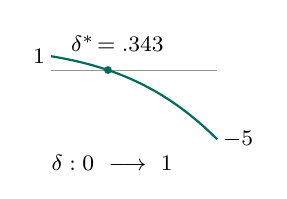
\begin{tikzpicture}[x=60pt,y=5pt,font=\fontsize{8}{9}\selectfont]
  \draw[pdinkmuted!55,line width=.35pt] (0,0)--(1,0);
  \draw[pdteal,line width=.8pt] plot[domain=0:1,samples=61]
    (\x,{1-2*(\x+\x*\x+\x*\x*\x)});
  \fill[pdteal] (.342508,0) circle[radius=1.4pt];
  \node[anchor=east,inner sep=2pt] at (0,1) {$1$};
  \node[anchor=west,inner sep=2pt] at (1,-5) {$-5$};
  \node[anchor=south,inner sep=3pt] at (.40,.7) {$\delta^*\!=.343$};
  \node[anchor=north west,inner sep=0pt] at (0,-6.1) {$\delta:0\ \longrightarrow\ 1$};
\end{tikzpicture}
\makeatother\endgroup
\par
Three-round model with no bond: net gain from deviation, in payoff units.
Above $\delta\approx.343$, deviation loses.}
The general sustainability condition under a $k$-round graduated trigger with stage-game payoffs $(u_C, u_D, u_P) = (3, 4, 1)$ and expected forfeiture $p_{\mathrm f}b$ is
\[
\underbrace{u_D - u_C - p_{\mathrm f}b}_{\text{one-shot gain}} \;<\; \underbrace{(u_C - u_P + p_{\mathrm f}b) \cdot \frac{\delta(1 - \delta^k)}{1 - \delta}}_{\text{discounted punishment cost}}.
\]
Substituting $u_D - u_C = 1,\; u_C - u_P = 2$ and $k = 3$ gives $1 - p_{\mathrm f}b < (2 + p_{\mathrm f}b)\,\delta(1 + \delta + \delta^2)$. Its root, $\delta^\star_{k=3}(p_{\mathrm f}b)$, is the threshold. With no bond the condition is $1 < 2\delta(1 + \delta + \delta^2)$, which solves numerically to $\delta > \delta^\star_{k=3}(0) \approx 0.3425$; written without an argument, $\delta^\star_{k=3}$ means this zero-bond value, the one the figures and the mechanized checks use. An expected forfeiture of $p_{\mathrm f}b = 0.5$, half the one-shot gain, lowers the threshold to about $0.1673$, and at $p_{\mathrm f}b = 1$ it reaches $0$ [verified]. Under grim trigger ($k \to \infty$), strict deterrence requires $\delta > (1 - p_{\mathrm f}b)/3$, which is $1/3 \approx 0.333$ with no bond. The three-round threshold is at most about $0.009$ higher. Finite punishment allows a return to cooperation after three compliant rounds; the calculation says nothing about crashes or mistaken observations.

\begin{pdclaim}{Theorem}{Claim Signaling Incentive Compatibility}
\setlength{\parskip}{4pt plus 1pt}
\label{prop:claim-signaling-ic}
Let the players be two principals with persistent identities that cannot escape the stated punishment. Assume the payoffs in Table~\ref{tab:claim-stage-game}; a bond under which every false claim, in every round, forfeits $p_{\mathrm f}b$ in expectation, with $0\le p_{\mathrm f}b<1$; and perfect public monitoring: both players observe the same past actions before each new round.

Under the three-round graduated-trigger strategy described above, cooperative truthful signaling is a subgame-perfect equilibrium for $\delta>\delta^\star_{k=3}(p_{\mathrm f}b)$, the unique root in $(0,1)$ of
\[
(2+p_{\mathrm f}b)(\delta^3+\delta^2+\delta)-(1-p_{\mathrm f}b)=0.
\]
With no bond this is $2\delta^3+2\delta^2+2\delta-1=0$, and $\delta^\star_{k=3}(0)=0.3425080314\ldots$; at $p_{\mathrm f}b=0.5$ the root is $0.1673\ldots$. Under grim trigger, the weak incentive condition is $\delta\ge(1-p_{\mathrm f}b)/3$. If $p_{\mathrm f}b\ge1$, truthful signaling is a dominant stage action and needs no punishment.

The ledger and identity mechanisms motivate these hypotheses but do not establish them for every deployment.
\end{pdclaim}

\begin{proof}
\setlength{\parskip}{4pt plus 1pt}
The public punishment counter, zero to three, is the only state. By the one-shot deviation principle for discounted games with bounded payoffs, the profile is subgame-perfect if no single deviation, followed by a return to the profile, pays in any state. In the cooperation state a deviation gains $1-p_{\mathrm f}b$ now and starts three punishment rounds, each $2+p_{\mathrm f}b$ below cooperation, so it does not pay when $1-p_{\mathrm f}b\le(2+p_{\mathrm f}b)(\delta+\delta^2+\delta^3)$. The left side of the displayed equation is strictly increasing in $\delta$, negative at $0$ and positive at $1$, so its root in $(0,1)$ is unique, and the inequality holds strictly above it. In a punishment state the prescribed $(F,F)$ is the stage game's Nash equilibrium, because $p_{\mathrm f}b<1$. Switching to $T$ there earns $0$ instead of $1-p_{\mathrm f}b>0$ in that round and restarts the counter at three, so it loses both now and later. Grim trigger replaces the three-round sum by $\delta/(1-\delta)$. If $p_{\mathrm f}b\ge1$, each $F$ payoff is at most the $T$ payoff against the same action, so $T$ is dominant.
\end{proof}

\begin{pdboundary}
\setlength{\parskip}{4pt plus 1pt}
This calculation assumes \emph{perfect public monitoring}: before choosing the
next round's action, both players know the same correctly observed action history.


A single-writer ledger supplies an unambiguous commit order, but does not ensure
timely delivery, complete observation of real actions, or agreement about a
round boundary. Those remain assumptions even inside one harbor. A protocol
could require both parties to read the same committed round before advancing;
no deployed protocol does this yet.

With noisy or private observations, the stated trigger can punish an action the
other party did not observe and provoke further punishment. This risk is not a
general impossibility theorem for cooperation.

Green and Porter
\pdcite{greenporter1984} study imperfect monitoring; Kandori and Matsushima
\pdcite{kandorimatsushima1998} study private observation with communication.
Their results depend on their own signal and communication models, not merely
on adding a witness log. Re-deriving this mechanism under delayed or private
monitoring remains \emph{open}, within a harbor as well as across harbors.
\end{pdboundary}

\paragraph{Where the argument stops.}
Removing an assumption invalidates this strategy's guarantee, not every possible cooperation mechanism.
\begin{itemize}[nosep]
  \item \emph{Remove the shared action history (\S\ref{sec:attribution}).} The prescribed trigger can no longer identify when punishment starts or ends. A Merkle forest can authenticate recorded evidence; it is not the only possible monitoring mechanism, and authentication alone does not deliver perfect public monitoring.
  \item \emph{Allow costless identity resets (\pdchapref{anchor}{The Anchor Protocol}).} If a principal can discard its identity and return immediately on unchanged terms, identity-specific punishment loses its force. Re-entry costs or a larger bond may change that incentive. An agent process that persists is not a persistent player; the principal is.
  \item \emph{Drop $\delta$ below $\delta^\star_{k=3}(p_{\mathrm f}b)$.} The three-round trigger no longer deters defection. For $(1-p_{\mathrm f}b)/3<\delta<\delta^\star_{k=3}(p_{\mathrm f}b)$, a sufficiently long finite punishment restores deterrence. At $\delta=(1-p_{\mathrm f}b)/3$, only the perpetual-punishment limit reaches the weak incentive condition; no finite window suffices.
  \item \emph{Drop $\delta$ below $(1-p_{\mathrm f}b)/3$.} Even perpetual mutual-$F$ punishment cannot deter a deviation from $(T,T)$ with these payoffs. No finite window of that punishment can do better. A larger expected forfeiture lowers this bound, and $p_{\mathrm f}b\ge1$ removes it.
\end{itemize}

Section~\ref{sec:youle:a6} reuses the same pattern at the insurer pricing layer: a stage game, a repeated game made possible by observable history, a deviation calculation, and a $\delta$ threshold. The analogy is one of structure only. No result carries over, because the payoff functions, monitoring signal, detection timing and punishment rules differ and must each be derived.

\paragraph{Mechanized claim-signaling.} The zero-bond case of the argument is also checked by machine. With $p_{\mathrm f}b=0$ the discount-factor threshold $\delta^\star$ is the unique real root in $(0,1)$ of $2\delta^3 + 2\delta^2 + 2\delta - 1 = 0$, numerically $\delta^\star \approx 0.3425$ (matching $\delta^\star_{k=3}$ above). The cubic, the existence-and-uniqueness of its root in $[0.34,\,0.35]$, and a TLA$^{+}$ model checking that no one-shot deviation produces positive discounted payoff at $\delta = 0.35$ are mechanized as \texttt{proofs/economics/delta-threshold.z3} and \texttt{proofs/economics/claim\_signaling.tla}. Both run unattended in CI (\S\ref{app:mech}, Table~\ref{tab:verification-status}). Neither models the bond; the frontier for $p_{\mathrm f}b>0$ rests on the derivation above.

The TLA$^{+}$ witness uses a shared countdown for one deviation followed by
compliant punishment. It does not exhaust arbitrary deviation histories or
the reset rule above; those belong to the analytical strategy argument.

\pdexercisepointerone*{\ref{ex:bonded-claim-signaling-pd}}{\pageref{ex:bonded-claim-signaling-pd}}

\begin{pdexample}{The Claim-Signaling Threshold}
\setlength{\parskip}{4pt plus 1pt}
Evaluate the zero-bond cubic $g(\delta) = 2\delta^3+2\delta^2+2\delta-1$ at $\delta=0.3425$ by hand, using the factored form \[
g(\delta)=2\delta(1+\delta+\delta^2)-1
\] to keep the arithmetic to two multiplications.

First \[
\begin{aligned}
\delta^2 &= 0.3425 \times 0.3425 = 0.11730625,\\
\text{ so }1+\delta+\delta^2 &= 1 + 0.3425 + 0.11730625\\
&= 1.45980625.
\end{aligned}
\]

Then $2\delta = 0.685$, and \[
\begin{aligned}
0.685 \times 1.45980625 &= 0.9999672813\ldots,\\
\text{ so }g(0.3425) &\approx 0.9999672813 - 1\\
&= -0.0000327
\end{aligned}
\] [verified].

That is within $3.3\times10^{-5}$ of zero, close enough to call $0.3425$ a root by hand, and the small \emph{negative} residual is consistent with the more precise value \texttt{delta-threshold.expected.txt} reports, $\delta^\star \approx 0.3425080314$: since $g$ is strictly increasing for $\delta>0$ (every term has a positive coefficient), a negative value at $0.3425$ means the true root sits slightly \emph{above} it, and $0.34250803 > 0.3425$ by exactly the sliver this residual predicts.

\emph{Now you try:} Exercise~\ref{ex:bonded-threshold-hand} asks you to bound the same root between two adjacent points of the $0.01$-step grid the model checker uses ($\delta=\texttt{DeltaNum}/100$) instead of evaluating it at the algebraic value alone.
\end{pdexample}

Figure~\ref{fig:bc-delta-threshold} plots that zero-bond root where it means
something: the deviator's own net payoff with no bond, against $\delta$, for
the graduated trigger and for grim trigger on the same axis.

% Analytic gain functions: U3=1-2(delta+delta^2+delta^3), Uinf=1-2delta/(1-delta).
% Map: x=38+244*delta pt, y=100-28*gain pt (downward-positive canvas).
% Full finite domain [0,1]; grim stops at gain=-5.3, then a short continuation.
% Archived TLC delta=.30: (441700000-425100000)/100^4 = .166.
\begin{figure}[H]
\centering
\begingroup
\SGMeasuredFigure{bc-delta-threshold}{%
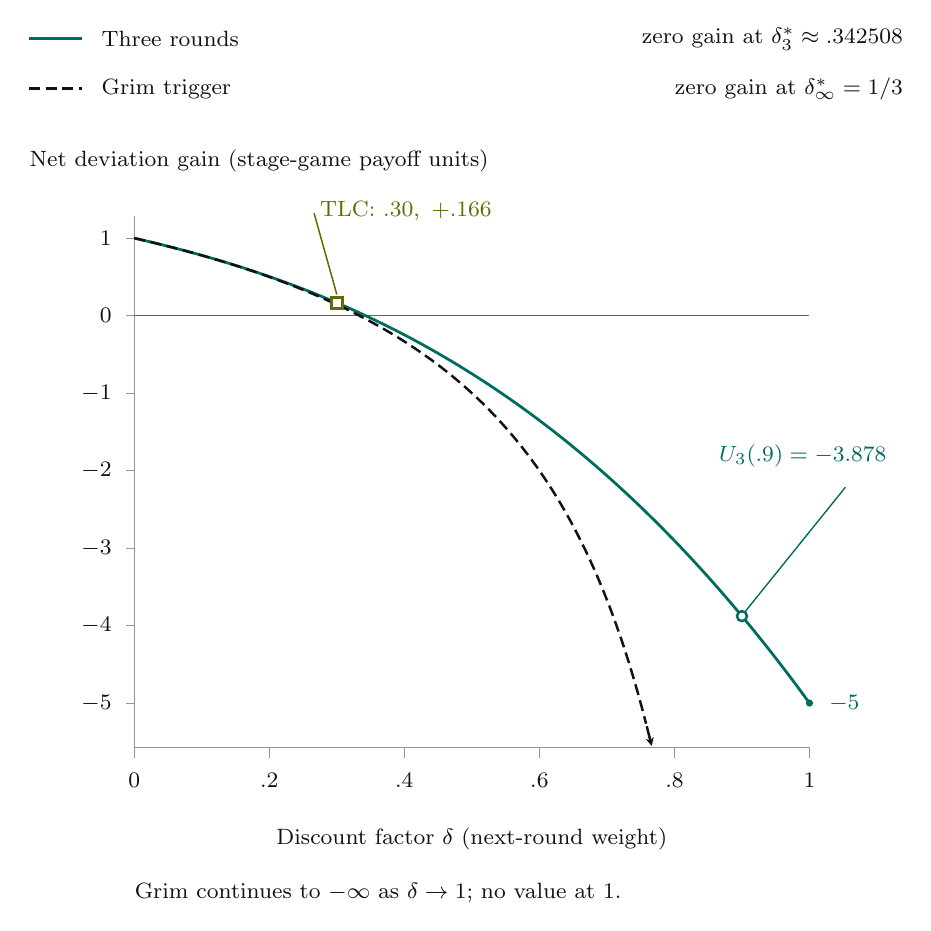
\begin{tikzpicture}[x=1pt,y=-1pt,font=\small,text=pdink,
  bc note/.style={font=\footnotesize,inner sep=0pt,align=left},
  bc axis/.style={draw=pdink!45,line width=.4pt}]
% Reserved comparison key: line styles and distinct zero-gain thresholds.
\draw[pdteal,line width=1pt] (0,0)--(19,0);
\node[bc note,anchor=west] at (26,0) {Three rounds};
\node[bc note,anchor=east] at (316,0) {zero gain at $\delta^*_3\approx.342508$};
\draw[pdink,line width=.9pt,dash pattern=on 4pt off 2pt] (0,18)--(19,18);
\node[bc note,anchor=west] at (26,18) {Grim trigger};
\node[bc note,anchor=east] at (316,18) {zero gain at $\delta^*_\infty=1/3$};
\node[bc note,anchor=west] at (0,44) {Net deviation gain (stage-game payoff units)};
% Both policies share these scales; zero, not the bottom, is indifference.
\draw[bc axis] (38,64)--(38,256)--(282,256);
\draw[pdink!65,line width=.45pt] (38,100)--(282,100);
\foreach \gain in {1,0,-1,-2,-3,-4,-5}{
  \draw[bc axis] (35,{100-28*\gain})--(38,{100-28*\gain});
  \node[bc note,anchor=east] at (30,{100-28*\gain}) {$\gain$};}
\foreach \delta in {0,.2,.4,.6,.8,1}{
  \draw[bc axis] ({38+244*\delta},256)--({38+244*\delta},260);
  \node[bc note,anchor=north] at ({38+244*\delta},265) {$\delta$};}
\draw[pdteal,line width=1pt]
  plot[domain=0:1,samples=121] ({38+244*\x},{100-28*(1-2*(\x+\x*\x+\x*\x*\x))});
\draw[pdink,line width=.9pt,dash pattern=on 4pt off 2pt]
  plot[domain=0:0.7590361446,samples=121] ({38+244*\x},{100-28*(1-2*\x/(1-\x))});
% Continue the grim curve along its downward tangent, above the tick-label rail.
\draw[pdink,line width=.9pt,-{Stealth[length=3pt,width=3pt]}]
  (223.205,248.4)--(225,255.5);
% The square is an archived finite-model witness, not a sample from a market.
\filldraw[fill=white,draw=pdgold,line width=1pt] (109.2,93.352) rectangle (113.2,97.352);
\draw[pdgold,line width=.55pt] (111.2,92.35)--(103,63);
\node[bc note,anchor=south west,text=pdgold] at (105,66) {TLC: $.30,\ +.166$};
% The open circle is the chapter's worked point on the finite curve.
\filldraw[fill=white,draw=pdteal,line width=.9pt] (257.6,208.584) circle[radius=1.8pt];
\draw[pdteal,line width=.5pt] (258.8,206.9)--(295,162);
\node[bc note,anchor=south east,text=pdteal] at (310,155) {$U_3(.9)=-3.878$};
\fill[pdteal] (282,240) circle[radius=1.3pt];
\node[bc note,anchor=west,text=pdteal] at (289,240) {$-5$};
\node[bc note,anchor=north] at (160,285) {Discount factor $\delta$ (next-round weight)};
\node[bc note,anchor=north west] at (38,305)
  {Grim continues to $-\infty$ as $\delta\to1$; no value at $1$.};
\end{tikzpicture}}
\endgroup
\caption{Three-round punishment caps the loss; grim punishment does not.
The curves assume shared, correct observations and no bond. The square is the archived
four-round TLC counterexample, not a measured payoff series.}
\label{fig:bc-delta-threshold}
\end{figure}

% Finish the deferred plot before starting the breakable recorded transcript.
\FloatBarrier

Below the threshold the model checker reports the failure and hands back the
deviation that causes it. At $\delta=0.30$ the honest score and the deviator's score are printed round by
round, and the run ends with the deviator ahead.

% GENERATED by scripts/harbor-research/record_sessions.sh -- do not edit.
\begin{pdsession}[claim signaling at \(\delta = 0.30\): TLC finds the profitable deviation]
$ java -cp tla2tools.jar tlc2.TLC -config claim_signaling_delta30.cfg claim_signaling.tla
Error: Invariant NoUnilateralDeviationPositive is violated.
Error: The behavior up to this point is:
State 1: <Initial predicate>
/\ deviatorId = "none"
/\ actualScore = [A |-> 0, B |-> 0]
/\ round = 0
/\ punishCountdown = 0
/\ deviated = FALSE
/\ followScore = [A |-> 0, B |-> 0]

State 2: <ChooseDeviator>
/\ deviatorId = "A"
/\ actualScore = [A |-> 0, B |-> 0]
/\ round = 0
/\ punishCountdown = 0
/\ deviated = FALSE
/\ followScore = [A |-> 0, B |-> 0]

State 3: <Step>
/\ deviatorId = "A"
/\ actualScore = [A |-> 400000000, B |-> 0]
/\ round = 1
/\ punishCountdown = 3
/\ deviated = TRUE
/\ followScore = [A |-> 300000000, B |-> 300000000]

  ... states 4-5 elided ...

State 6: <Step>
/\ deviatorId = "A"
/\ actualScore = [A |-> 441700000, B |-> 41700000]
/\ round = 4
/\ punishCountdown = 0
/\ deviated = TRUE
/\ followScore = [A |-> 425100000, B |-> 425100000]

10 states generated, 10 distinct states found, 1 states left on queue.
The depth of the complete state graph search is 6.
Finished in 00s
\end{pdsession}



\pdexercisepointer*{\ref{ex:bonded-threshold-hand}}{\ref{ex:bonded-sweep-crossover}}{\pageref{ex:bonded-threshold-hand}}

\begin{pdrecitation}
\item Without looking: what is the one-shot Nash equilibrium of the stage game in Table~\ref{tab:claim-stage-game}, and why does that rule out truthful signaling as an equilibrium of this one-shot payoff table?
\item Name the three ingredients the repeated game needs to sustain truth-telling, and which section of the chapter supplies each one.
\item Which polynomial defines the threshold $\delta^\star_{k=3}(p_{\mathrm f}b)$ for the three-round graduated trigger, and what does a larger expected forfeiture do to it?
\end{pdrecitation}

% Stranded at the foot of p. 358 in all three editions (p. 362 Swiss). Same
% reservation as the other one: the heading travels with its first paragraph.
\needspace{7\baselineskip}
\subsection{Pricing the Bond}\label{sec:pricing}

What is the right collateral for ``write access to \texttt{auth.ts} for 30 minutes''? The answer requires a pricing function $\pi: \mathcal{F} \rightarrow \mathbb{R}^{+}$ that maps Float Plans to bond amounts. An effective $\pi$ must satisfy:

\begin{enumerate}[nosep]
  \item \textbf{Deterrence}: expected collectible loss must exceed the
principal's gain from deviation. If gain $G$ is retained and the bond is
forfeited with probability $p_{\mathrm f}$, the two-action test is $p_{\mathrm f}\pi(\mathcal F)>G$.
Damage and private gain need not coincide.
  \item \textbf{Accessibility}: $\pi(\mathcal{F})$ must not be so high that legitimate agents are priced out of the commons.
  \item \textbf{Risk sensitivity}: $\pi$ should increase with the scope and criticality of the manifest.
  \item \textbf{History adjustment}: $\pi$ may decrease for principals with strong track records.
\end{enumerate}

We do not close this problem. We tighten the lower bound, propose a scope multiplier, suggest a reputation discount, and describe two concrete mechanisms: the \pdterm{Bonded Advisor}, an agent that proposes bond sizes and is itself bonded on their accuracy (\S\ref{sec:bonded-advisor}), and Youle's competitive-insurance market (\S\ref{sec:youle}). The repair in \S\ref{app:worked} sized its \$6 bond this way, from a \$5 cleanup bill and a $20\%$ scope uplift.

\subsubsection{Cleanup Lower Bound}\label{sec:cleanup-bound}

Let $c$ be the project's cleanup cost, the human and compute cost to detect, assess and recover from one breach. It can be read from the audit log.
\pdmarginanalogy{batch3-ch07-repair-kit}{}{ch07-cleanup-repair-kit}{Like repairing a damaged fitting, cleanup consumes work and materials after the breach.}%

\begin{pdclaim}{Theorem}{Cleanup Lower Bound}
\setlength{\parskip}{4pt plus 1pt}
\label{thm:cleanup-bound}
If each breach costs the commons a fixed $c>0$, and full forfeiture of the
collectible bond is its only source of cleanup funding, avoiding a deficit
on every breach requires $\pi(\mathcal F)\ge c$.
\end{pdclaim}

\begin{proof}[Rationale]
\setlength{\parskip}{4pt plus 1pt}
If $\pi(\mathcal{F}) < c$, breach is cheap: the bond is forfeit for less than the cleanup cost. If the commons pool funds cleanup, $\pi < c$ drains the commons on every breach, and the system bankrupts itself through enforcement.

\qed

\paragraph{When the fixed cleanup bill is inadequate.}
The fixed-cost model assumes a bounded cleanup bill. It is inapplicable to unbounded or poorly controlled tail losses (e.g., dropping a production database or leaking a private key). A finite bond cannot guarantee full compensation for an unbounded loss. Defense of these tasks is explicitly moved to Layer 1 capability confinement (isolation domains, zero-egress policies); the cost-recovery calculation applies only to the bounded loss it actually models.
\end{proof}

The theorem gives a lower bound for recovering cleanup costs under the stated
funding rule; it says nothing about deterrence. With $c=5$, a fully collected
bond of $6$ covers cleanup. If sabotage
gives the principal $10$ and is caught half the time, its expected gain is
still $10-0.5(6)=7$. Coverage and deterrence are separate calculations.
Historical cleanup records estimate $c$; they do not bound every future loss.

\subsubsection{Consequential-Scope Multiplier}\label{sec:scope-multiplier}

Let $s(\mathcal{F})$ be plan scope (files claimed, presence of \texttt{db:write}, production-deployment capability). One candidate schedule raises the bond linearly with scope.
It is a proposal to calibrate, not a measured relationship.
\[
\pi(\mathcal{F}) \;\geq\; c \cdot \bigl(1 + \eta \cdot s(\mathcal{F})\bigr).
\]
$\eta$ is calibrated from observed cleanup per scope unit. Low-$\eta$ projects have simple, easily-audited work; high-$\eta$ projects have tangled dependencies. $\eta$ is publishable from the audit log.

\subsubsection{Reputation Discount}\label{sec:rep-discount}

If a calibrated model predicts lower future damage for a principal with
clean settlements, a proposed discount is:
\[
\pi(\mathcal{F}, P) \;=\; \max\{c,\,\pi(\mathcal{F})(1-\lambda(P))\},
\quad \lambda(P) \in [0, \lambda_{\max}],\; \lambda_{\max} \leq 0.5,
\]
while keeping the bond at or above $c$. A raw quote of $6$ with a $50\%$
discount would be $3$; if $c=5$, the posted bond is $5$, not $3$. $\lambda$ increases with clean settlements, decreases with breaches, decays over time. The functional form is left open.

\subsubsection{Threat-Class Bond Sizing}\label{sec:pricing:threats}

The closed-form bond $\pi(\mathcal{F}, P) = \max\{c,c(1 + \eta s)(1 - \lambda)\}$ prices every threat from the same cleanup-cost curve. One calibration may not serve every task: a price intended to deter costly sabotage can exclude providers from low-exposure work, while an accessible price may leave severe losses underfunded. Task permissions, recoverability and loss estimates therefore matter alongside the multiplier.

Table~\ref{tab:threat-bonds} gives illustrative starting bands. The first three are shares of the \pdterm{claim ceiling} (the most that will be paid out on a claim), not validated coverage levels; the exfiltration row is a lower bound derived below. Careless work means an attempted result that is sloppy, partial or fails review; abandonment means leaving accepted work unfinished; sabotage means deliberate damage to shared state. These descriptions classify outcomes for analysis; they do not test intent.

\begin{table}[H]
\centering
\caption{Illustrative bond bands. The first three rows are percentages of the claim ceiling; the exfiltration row is a lower bound set by detection power. These are calibration proposals, not protocol constants or loss guarantees.}
\label{tab:threat-bonds}
\setlength{\tabcolsep}{3pt}
\begin{tabularx}{\textwidth}{@{}>{\raggedright\arraybackslash}p{2.6cm}>{\raggedright\arraybackslash}p{2cm}>{\raggedright\arraybackslash}X@{}}
\toprule
\textbf{Threat} & \textbf{Bond} & \textbf{Intended purpose} \\
\midrule
Careless work & 10--25\% & Encourage care with affordable entry. \\
Abandonment & 25--50\% & Help fund replacement onboarding. \\
Active sabotage & 100--200\% & Help fund reconstruction and cleanup. \\
Data exfiltration & $\ge c_{\mathrm x}/p_{\mathrm f}$ & Fund detection and response only; disclosure is not covered. \\
\bottomrule
\end{tabularx}
\end{table}

An abandonment reserve aims to pay for scope-note ingestion, partial-diff review and salvage handoff. Coverage requires a measured cost bound (\S\ref{sec:attribution-survives}). A sabotage reserve aims to fund reconstruction and downstream cleanup; a percentage of the claim ceiling bounds neither loss, and even a bond above the ceiling may underfund reconstruction. The careless-work band likewise proposes an incentive, not a demonstrated reduction in failures. Each band requires calibration against attributable outcomes and observed costs.

The exfiltration row prices something narrower than the leak. A bond cannot retract disclosed information, and the loss or an attacker's gain can exceed any collectible collateral, so the row does not cover the disclosure. It funds only detecting and responding to a leak, the scope \pdchapref{sealed}{The Sealed Harbor} gives it. Let $c_{\mathrm x}$ be the exfiltration counterpart of the cleanup cost $c$: the expected cost of detecting and responding to one leak, not counting the harm of the disclosure itself. The bond is forfeited only if the leak is detected and the bond collected. Call that probability $p_{\mathrm f}$; it is at most the detection power of the sealed harbor's canary theorem\ifpdbook\ (Theorem~\ref{sealed:thm:sealed-power})\fi. The expected forfeiture per leak is then $p_{\mathrm f}\pi(\mathcal F)$, and the Cleanup Lower Bound becomes
\[
\pi(\mathcal F)\;\ge\;\frac{c_{\mathrm x}}{p_{\mathrm f}}.
\]
An undetected leak forfeits nothing, so no finite bond avoids a deficit on every leak; this bound covers $c_{\mathrm x}$ on average over leaks. In the sealed harbor's recorded example, with $100$ canaries among $10^4$ records and a per-canary miss rate of $0.2$, a $100$-record leak is detected with probability $0.554$, so the bond must be at least $1/0.554\approx1.8$ times $c_{\mathrm x}$. That power assumes each canary is missed independently. If a deliberate exfiltrator's misses are perfectly correlated, the power falls to $0.509$ and the multiplier rises to about $2.0$. Small leaks are where the bound stops being practical: at the same canary density a one-record leak is detected with probability $0.008$, and the bound asks for $125c_{\mathrm x}$ [verified]. Preventing disclosure still requires mediated access and egress controls with their own threat model; ordinary worktrees do not provide confinement (\S\ref{sec:isolation}).

The table informs Phase~2 below through exposure limits: restrict the resources and task value entrusted to a new principal, then reconsider those limits after attributable settlements. A newcomer can still act maliciously. An access tier limits what can be reached or lost; it does not restrict a principal to careless work or certify benign intent.

\subsubsection{Bootstrap Path}\label{sec:pricing:bootstrap}

Competitive insurance (\S\ref{sec:youle}) works only in a busy market. It needs insurers with capital, principals with reputation history, and enough transaction volume that bidders can statistically distinguish good risks from bad. A cold-start deployment may lack all three. The cohort sizes and thresholds
below are illustrative operating proposals, not measured readiness tests. The conditional comparison of the auction with a static baseline (\S\ref{sec:youle:welfare}) describes the modeled end state; Phases~1--2 below are the path to the assumptions it needs.

\paragraph{Phase 1: Subsidized seeding.}
The marketplace operator posts real tasks at above-market rates and invites a small cohort of $5$--$10$ known-capable principals from an existing network. Bonds are fixed at a flat rate per task class; pricing is not a parameter to optimize yet, because there is no data to optimize against. The goal is to produce the first row of the reputation table: clean settlements, breaches, recovery times, observed cleanup cost $c$. The operator is subsidizing the existence of an audit log.

\emph{Transition metric.} Completion rate above $80\%$ sustained for $\geq 2$ consecutive weeks. Usable risk estimates also need checks of sample size,
selection, loss severity and uncertainty.

\paragraph{Phase 2: Complexity-proportional pricing with graduated access.}
The closed-form bond $\pi(\mathcal{F}, P) = \max\{c,c(1 + \eta s)(1 - \lambda)\}$ activates, with $\eta$ calibrated from Phase~1 cleanup data and $\lambda$ initialized from the Phase~1 reputation table. New principals enter a tier with limited permissions and task value, using the lower bands of Table~\ref{tab:threat-bonds} as pricing proposals. Access to greater exposure is reconsidered after accumulated clean settlements, mirroring the A5 composite mechanism (\S\ref{sec:youle:a5}); neither the bond band nor the history rules out malicious conduct.

Reputation bootstrapping is the hard problem of this phase. A principal with verifiable work history from another deployment should not start at zero, but the operator cannot verify external histories directly. The proposed mechanism imports attestations: external audit trails signed under an Anchor-issued key (\S\ref{sec:attribution}) earn partial reputation credit, capped well below an equivalent in-system history. The credit is partial because cross-deployment reputation does not control for local cleanup cost, and capped because a fraudulent attestation issuer is a single point of failure.

\emph{Illustrative investigation signal.} New-principal $30$-day retention
below $50\%$ would prompt review of access gates, bond prices, task value and
other causes of churn. Retention is read alongside loss, participation and
calibration evidence; on its own it says nothing about readiness for
competitive bidding.

\paragraph{Phase 3: Competitive insurance.}
The \S\ref{sec:youle} mechanism activates: insurer agents bid on underwriting transactions, static parameters retire as insurer volume grows, and listing fees enable the cartel-resistance regime of \S\ref{sec:youle:a6}. The operator's pricing parameters become fallbacks rather than the primary mechanism; they apply only when fewer than a threshold number of insurer bids arrive on a transaction.

\emph{Transition metric.} Repeat-poster rate above $60\%$. The competitive-insurance equilibrium of \S\ref{sec:youle:welfare} assumes repeated interaction; repeat activity may help recover information costs.
Competitive entry and risk calibration still need their own evidence.

\medskip

The weak-improvement result of \S\ref{sec:youle:welfare} is conditional on Phase~3 being reached, the listed metrics being met, and the specified full-information, competitive-entry, coverage, and static-baseline assumptions holding. Phases~1--2 generate the data the competitive-insurance market needs to price at all. A deployment that skips them is running \S\ref{sec:youle} on uninformative priors, and the comparison does not apply.

\subsubsection{Settlement and Dispute}\label{sec:pricing:settlement}

The settlement design needs an adjudication rule distinct from lifecycle
status. Neither a missed heartbeat nor the TLA$^{+}$ excerpt itself determines
a slash. Attribution is recorded (\S\ref{sec:attribution}), and the agreed
appeal window permits challenge. That is most of what is needed, but it makes the daemon the verifier, the judge and the arbiter of evidence at once, a position no single component should hold. We call any evaluator whose verdict a settlement relies on an oracle. Strong evidence does not make a single oracle correct; it makes it confidently wrong in the cases where its evidence is incomplete.

One proposal separates three evaluators with different costs and failure
modes. Their agreement is useful only under an explicit rule for missing
verdicts, correlated errors and appeals.

\paragraph{Oracle 1: Automated.}
Test-suite pass/fail, type checks, lints, coverage thresholds, and any deterministic CI signal already recorded on the session. Cheap to run, fast to return, and \emph{gameable}: a principal who knows the test surface can ship work that passes the checks while failing the intent. The daemon already produces this oracle as a side effect of normal operation; the change is to label it as one signal among three rather than the dispositive one.

\paragraph{Oracle 2: Evidence-based.}
A verifier (which may itself be a bonded agent) reviews the Merkle attribution chain (\S\ref{sec:attribution}) for the disputed transaction. The chain is append-only and cryptographically bound, so the oracle's hard problem is not authenticity of the evidence but interpretation: did the recorded actions match the Float Plan's scope, and do the diffs produced match the acceptance criteria? Medium cost; authentic records can still be incomplete or misleading, and collusion adds another failure mode (\S\ref{sec:youle:a5}).

\paragraph{Oracle 3: Human audit.}
A randomized sample of contested settlements, at a configurable rate (default $10\%$), is routed to a human auditor. Expensive, slow, and authoritative. The audit produces a labeled outcome that feeds back into reputation history and into calibrating Oracles 1 and 2: any disagreement between human audit and the cheaper oracles is a training signal for the gameable layers.

\paragraph{Settlement rule.}
A sampled human audit is not a third vote on every case. The contract must
name the unsampled path. One proposed rule is: when the two automated oracles
agree, record a provisional verdict under the agreed appeal window; when
they disagree or abstain, hold the bond for human arbitration. Sampled cases
also receive a human review. If all three verdicts exist, a 2-of-3 rule can
produce the provisional outcome, with dissent retained for appeal. Final
human authority and reversal funding must be agreed in advance. This is a
protocol proposal; sampling does not give every case a majority review or
make any evaluator infallible.

\paragraph{Composition with cartel resistance.}
Oracle collusion is itself a collusion problem. If Oracles 1 and 2 are run by agents in the same cartel, their 2-of-3 majority can launder a sabotaged settlement past the human audit unless the audit happens to sample it. The same insurer-collusion analysis applies (\S\ref{sec:youle:a6}) with the oracles in the role of bidders: the human-audit sampling rate $\xi$ sets the detection probability $p_d^{\text{oracle}} = \xi d_{\mathrm h}$, where $d_{\mathrm h}$ is the conditional probability that a sampled audit detects misconduct for the oracle layer, and the folk-theorem threshold becomes a calibration target on $\xi$ in the same way it is a calibration target on bid-pattern detection elsewhere in the protocol. The default $10\%$ sample is a starting point; deployments where Oracles 1 and 2 are co-owned should raise it.

\subsubsection{The Bonded Advisor}\label{sec:bonded-advisor}

One direction for solving $\pi$ is to delegate its computation to a specialized agent that is itself bonded on the accuracy of its advice, the Bonded Advisor:
\begin{itemize}[nosep]
  \item A principal posts a Float Plan whose only acceptance criterion is ``propose a fleet that meets budget/scope constraints for project $Q$.''
  \item A Bonded Advisor surveys $Q$ and emits a candidate fleet, itself a set of Float Plans with proposed $\pi$ values.
  \item The advisor's bond on the proposing plan is slashed proportionally to the accepted fleet's eventual breach rate. Clean settlements accumulate reputation; breaches shrink it.
\end{itemize}

\pdmarginanalogy{bonded-shear-pin}{}{ch07-shear-pin-fuse}{Like a drive shaft shear pin designed to snap under catastrophic overload to protect the engine, slashing liquidates posted collateral to protect the commons when a contract is breached.}%
The pricer is itself priced. The advisor that sets bond sizes posts a bond on its own accuracy. Whether this converges depends on (i) whether the advisor has access to sufficient prior-fleet audit data to pattern-match new projects, (ii) whether reputation history is long enough for discounting to be meaningful, and (iii) whether the population of advisors is large enough for competition to discipline outliers.

\paragraph{$c$ as a project health metric.} A project whose $c$ is rising is fraying. Breaches cost more to recover from, which suggests coordination in the project is decaying. The authority can publish $c$ alongside the bond pool and raise required bonds automatically when $c$ crosses a threshold. This is homeostatic feedback, like a body correcting its own temperature: risky spawns cost more exactly when the project can least afford them.

\paragraph{Threat-class bond bands and their defensibility.}\label{sec:pricing:defensibility}
For the three threat classes priced as shares of the claim ceiling, the pricing function $\pi$ resolves to one of three nominal bands, each calibrated to the threat class the bond is defending against:
\begin{itemize}[nosep]
  \item \textbf{Careless} (accidental damage during honest attempts): $\pi \in [10\%,\,25\%]$ of the claim ceiling.
  \item \textbf{Abandonment} (walk-away mid-task; cleanup dominates): $\pi \in [25\%,\,50\%]$ of the claim ceiling.
  \item \textbf{Sabotage} (intentional destruction; can exceed face value): $\pi \in [100\%,\,200\%]$ of the claim ceiling.
\end{itemize}
A Monte Carlo sweep over the cross product of seven plausible threat-distribution mixes and the three bands quantifies defensibility: for every \emph{matched} (mix, band) pair, where the mix concentrates on the class the band is designed to defend against, observed extraction stays within $1.10\times$ the band's upper bound (10\% stochastic tolerance). Off-diagonal cells (e.g. a sabotage-heavy mix posted against the careless band) are surfaced as widening recommendations rather than silent failures. The simulation is mechanized as \texttt{proofs/bonded/pareto/threat-bands.mjs} and runs on every PR (\S\ref{app:mech}, Table~\ref{tab:verification-status}).

\subsubsection{Competitive-Insurance Pricing Mechanism}\label{sec:youle}
\marginnote{Contributed by Thomas Youle, Indiana University, Business Economics
\& Public Policy, following conversations with the author in March--April
2026. The competitive-insurance mechanism and welfare comparison remain
a draft pending economist review.}
The mechanism adapts classical competitive-insurance market
models~\pdcite{rothschildstiglitz1976,wilson1977insurance} to agent transactions.

\paragraph{The mechanism.}\label{sec:youle:mechanism}
Instead of a static bond size $B_{\mathrm{static}}(\pi, \lambda, s)$ selected by the commons authority (\S\ref{sec:scope-multiplier}), let a market of insurer agents bid to underwrite each agent transaction. An insurer $I$ offers a quote $(q_I, c_I)$ where $q_I$ is the required premium and $c_I$ is the claim ceiling, the most the insurer will pay on a claim.

A principal $P$ submits a transaction $\mathcal{T}$ requiring total secured coverage
$B_T$. Insurers quote $0\le c_I\le B_T$; the principal selects one and
reserves the remaining $B_T-c_I$. For assessed damage $D\ge0$, settlement pays
\[
 I(D)=\min(D,c_I),\qquad
 P(D)=\min\bigl((D-c_I)_+,B_T-c_I\bigr).
\]
Thus $I(D)+P(D)=\min(D,B_T)$ when both parties perform; loss above $B_T$
remains uncovered. With $B_T=100$, $c_I=80$, and $D=90$, the insurer pays
$80$ and the principal $10$. Insurer default invokes its separately stated
collateral rule; a coverage promise alone is not a funded payout.

\paragraph{Market-discovered pricing.}
A cost-based quote has premium
$q_I=\mathbb E[\min(D,c_I)\mid \mathcal{T},\textit{history}]+\alpha_I$,
where $\alpha_I$ covers operating costs, capital, and risk. A zero-markup
competitive benchmark additionally assumes known risk classes, credible
payment, and sufficient competition. It is not a general consequence of
Rothschild--Stiglitz: adverse selection can prevent competitive equilibrium
from existing~\pdcite{rothschildstiglitz1976,wilson1977insurance}.

\paragraph{Adverse-selection controls.}
To avoid the lemons problem, in which only bad risks stay in the market because good ones find the price too high, the mechanism requires:
\begin{itemize}[nosep]
  \item Public agent reputation history (from the Merkle forest of \S\ref{sec:merkle-forest}).
  \item Principal-bound slashing if an agent's history is misrepresented at quote time.
  \item Insurer capital reserve backed by on-chain stake (the same bond mechanism, recursive: an insurer posts bond that its claim ceilings are funded).
\end{itemize}

\paragraph{Welfare comparison (model-conditional).}\label{sec:youle:welfare}
Under the simulation's full-information, competitive-entry assumptions and its chosen static baseline, the market-discovered premium can weakly improve the modeled principal and insurer payoffs while preserving coverage $B_T=\mu(1+\gamma)$, where $\mu$ is the transaction's expected loss and $\gamma$ the protocol's safety margin. This is not a claim against \emph{every} static parameter: a static price equal to the competitive price is outcome-equivalent, and transfers outside the modeled parties can change the Pareto ordering.


The accompanying Monte Carlo artifact sweeps 36 parameter configurations
(Appendix~\ref{app:mech}), with 2{,}000 trials of 50 transactions per
configuration. Figure~\ref{fig:pareto-mc-inline} plots the fraction of trials
passing the script's \emph{tolerance-based comparison}: principal cost is
strictly lower than under the static baseline, commons receipts are at least
97\% of that baseline's receipts, and aggregate insurer profit is at least
$-5\%$ of the baseline's principal cost. Because the latter two tests permit
losses, this success rate is not a test of exact Pareto dominance.

With five insurers and no colluders, the reported rate falls from $0.861$
at zero reputation noise to $0.006$ at $\sigma_r=0.3$. All three plotted
colluder counts have rates below $0.21$ at that noise level. The second
panel holds noise and collusion at zero: the rates are $0.906$, $0.861$ and
$0.739$ for three, five and ten insurers. More insurers therefore do not
improve this comparison in that slice of the simulation. These are
finite-sample results for the supplied implementation, baseline and
parameter grid, not general claims about auction efficiency.

% Brief (tikz-diagram-craft).
% Reader question: how does the simulation's tolerance-based comparison
%   change with reputation noise, colluder count and insurer count?
% Claim: for n=5 all three rates are below 0.21 at noise 0.3 and 0.5;
%   without noise or collusion, the plotted rate falls as n rises from 3 to 10.
% Evidence: proofs/bonded/pareto/simulation.mjs, simulation.run.log;
%   2000 trials of 50 transactions per configuration. Success requires
%   lower principal cost, commons receipts >=97% of the static amount,
%   and insurer profit >=-5% of static principal cost. This is not exact
%   Pareto dominance. Values are rounded to three decimals by the script.
% Must distinguish: the 0/1/3-colluder series; the two parameter sweeps;
%   simulation frequencies from general efficiency guarantees.
% Grammar: paired pgfplots axes on one rate scale, with a shared series key.
%   Rejected: a single curve varying noise and insurer count together,
%   which would confound the two sweeps.
% Five-second test: a reader identifies all three series and sees that
%   increased noise or more insurers need not improve this comparison.
\begin{figure}[H]
\centering
\pdfigurehue{pdgold}%
\begin{tikzpicture}[pd figure]
\begin{groupplot}[
  group style={group size=2 by 1, horizontal sep=1.05cm},
  pd axis,width=4.2cm,height=4.05cm,
  ymin=0,ymax=1,ytick={0,.25,.5,.75,1},
  yticklabels={0,.25,.5,.75,1},
]
\nextgroupplot[
  xlabel={reputation noise $\sigma_r$},
  title={A. Reputation noise},
  xtick={0,.1,.3,.5},
  legend columns=3,
  legend cell align=left,
  legend to name=pd-pareto-comparison-key,
]
  \addplot[pd ready series,mark=o] coordinates {(0,.861)(.1,.675)(.3,.006)(.5,.002)};
  \addlegendentry{0 colluders}
  \addplot[pd focus series,mark=square] coordinates {(0,.877)(.1,.916)(.3,.175)(.5,.075)};
  \addlegendentry{1 colluder}
  \addplot[pd breach series,mark=triangle] coordinates {(0,.926)(.1,.844)(.3,.208)(.5,.163)};
  \addlegendentry{3 colluders}
\nextgroupplot[
  xlabel={insurer count $n_I$},
  title={B. Insurer count},
  xtick={3,5,10},
]
  \addplot[pd ready series,mark=o] coordinates {(3,.906)(5,.861)(10,.739)};
\end{groupplot}
\node[pd label,rotate=90,anchor=south] at (-0.95,2.15) {Comparison success rate};
\end{tikzpicture}
\par\smallskip
\begin{tabular}{@{}c@{}}
\toprule
{\pdsetfocushue\pgfplotslegendfromname{pd-pareto-comparison-key}}\\
\bottomrule
\end{tabular}
\caption{Simulation frequencies for the tolerance-based comparison defined
in the text. A fixes $n_I=5$; B fixes noise and collusion at zero. Each point
uses 2{,}000 trials of 50 transactions.
[simulation, simulation.mjs]}
\label{fig:pareto-mc-inline}
\end{figure}


\paragraph{Relationship to the Bonded Advisor.}
Under this framing, the Bonded Advisor of \S\ref{sec:bonded-advisor} becomes the matchmaker plus reputation oracle in the insurance market. It does not set prices; it provides information. Competitive equilibrium is the pricing benchmark only under the market
and information assumptions stated above; the advisor does not establish
its existence.

\subsubsection{A5: A coverage cap bounds the deterrence from deposits}\label{sec:youle:a5}

An adversary funds $K$ insurer identities, underbids honest insurers, and
defaults when a covered loss occurs. The analyzed simulation uses a
\emph{coverage-capped} collateral rule
$\zeta(B_{\mathrm{dep}},B_T)=\min(B_{\mathrm{dep}},B_T)$.
Premiums are paid on every winning transaction, including defaults; capital
is replenished between transactions, and funding and entry costs are zero.
These assumptions specify the numerical experiment, not a complete
mechanism for insurer solvency or identity checks.

% Reader question: If one principal can fund many fake identities, how does
%   the mechanism keep a defaulting identity loss bounded?
% Claim: replicating identities multiplies entry cost, never the loss the
%   mechanism attaches to one default, because slash equals the lesser of the
%   posted deposit and the transaction coverage ceiling.
% Evidence: K interchangeable identities, each depositing B_dep; the closed
%   form s = min(B_dep, B_T) from this chapter section on Sybil deterrence
%   [internal, closed form].
% Must distinguish: entry cost (which rises with K) from attacker loss
%   (which does not rise past B_T no matter how many identities enter).
% Grammar chosen: identity fan-out beside its closed-form response curve.
%   Rejected: the atlas row prescribes an actor sequence with an accounting
%   rail; this page argues a bound on a formula, not an ordered sequence of
%   attacker actions, so the sequence grammar would misstate what this
%   fragment proves. Flagged for the author.
% Five-second test: a reader says slash stops rising once the deposit passes
%   the transaction coverage ceiling, no matter how many identities exist.
\begin{figure}[H]
\centering
\pdfigurehue{pdgold}%
\begin{tikzpicture}[pd figure,x=1cm,y=1cm]
  % ---- one grid -------------------------------------------------------------
  \def\px{0.85}  \def\py{1.35}
  \def\ix{2.75}
  \def\ax{3.55}  \def\bx{4.15}
  \def\ox{4.75}  \def\oy{0.15}
  \def\rx{7.35}  \def\xmax{7.75}  \def\ymax{2.40}
  \def\kx{6.45}  \def\ky{1.85}
  \node[pd title,anchor=north west,text width=6.0cm] at (0,4.45)
    {more identities require more posted capital};
  % ---- panel A: one principal fans out into K identities -------------------
  \node[pd identity state,circle,minimum size=8mm,inner sep=1pt] (pp) at (\px,\py) {$P$};
  \foreach \y/\lab in {2.55/1,1.95/2,1.35/3,0.75/{$\ldots$},0.15/{$K$}} {
    \node[pd identity state,circle,minimum size=6.5mm,inner sep=.5pt] at (\ix,\y) {\lab};
    \draw[pd identity rule,dashed] (pp.east) -- ({\ix-.42},\y);}
  \node[pd label,anchor=south] at (\ix,2.90) {$K$ insurer identities};
  \node[pd note,anchor=north,text width=3.6cm,align=center] at (\ix,-.46)
    {$K \times B_{\mathrm{dep}}$ posted; each identity can re-enter};
  \draw[pd focus arrow] (\ax,\py) -- (4.25,\py);
  % ---- panel B: the closed-form response, s = min(B_dep, B_T) --------------
  \draw[pd arrow] (\ox,\oy) -- (\xmax,\oy);
  \draw[pd arrow] (\ox,\oy) -- (\ox,\ymax);
  \node[pd label,anchor=west] at (\xmax,\oy) {deposit};
  \node[pd label,anchor=west] at ({\ox+.08},{\ymax+.16}) {slash $\zeta$};
  \draw[pd guide] (\kx,\oy) -- (\kx,\ky);
  \draw[pd guide] (\ox,\ky) -- (\kx,\ky);
  \node[pd label,anchor=north] at (\kx,{\oy-.10}) {$B_T$};
  \node[pd label,anchor=east] at ({\ox-.10},\ky) {$B_T$};
  \path[pd neutral fill] (\kx,\oy) rectangle (\rx,\ky);
  \draw[pd focus rule] (\ox,\oy) -- (\kx,\ky);
  \draw[pd focus rule] (\kx,\ky) -- (\rx,\ky);
  \node[pd focus datum] at (\kx,\ky) {};
  \node[pd label,anchor=south] at ({(\kx+\rx)/2},{\ky+.14}) {$\zeta=B_T$};
  \node[pd note,anchor=north,text width=3.5cm,align=center] at ({(\ox+\rx)/2},{\oy-.72})
    {extra deposit returns intact past $B_T$};
\end{tikzpicture}
\caption{Under the analyzed coverage-capped contract, extra identities
require extra posted capital. Slashing stops at coverage $B_T$; deposits above that cap cannot increase
the loss. Figure~\ref{fig:sybil-mc-inline} tests the resulting incentives.
[internal, closed form]}
\label{fig:sybil-inline}
\end{figure}


For a fixed transaction with premium $q$, loss probability $p>0$, and
coverage $B_T$, expected attacker profit under this contract is
\[
\mathbb E[\pi_{\mathrm{atk}}]=q-p\min(B_{\mathrm{dep}},B_T).
\]
If $q>pB_T$, no deposit increase deters this attack under the capped rule.
If $q\le pB_T$, deposits $B_{\mathrm{dep}}\ge q/p$ do deter it weakly.
This is a conditional limitation of the cap, not an impossibility theorem
for deposits. Under full forfeiture instead, the same premium convention
gives $\mathbb E[\pi_{\mathrm{atk}}]=q-pB_{\mathrm{dep}}$, so $B_{\mathrm{dep}}\ge q/p$
is sufficient in this one-shot model. For $q=10$, $p=0.1$, and $B_T=20$,
a deposit of $110$ gives profit $8$ with the cap and $-1$ with full forfeiture.
If the premium is also clawed back on default, both formulas change.

The seeded sweep in Figure~\ref{fig:sybil-mc-inline} tests the capped
contract only: its tested deposits from $0.5$ to $1000$ remain profitable
for its stipulated bids and loss distribution. Those bids use a loss-size
parameter rather than actuarially fair expected payouts. The experiment
therefore demonstrates a failure of that particular pricing-and-collateral
combination; it does not estimate a competitive insurer equilibrium.

% Brief (tikz-diagram-craft).
% Reader question: does raising the per-identity Sybil deposit ever make
%   the attack unprofitable, and what happens to the commons' own losses?
% Claim: attacker net profit stays positive across the whole tested deposit
%   sweep (0.5 to 1000 USD) for both one and three Sybil identities, while
%   the commons' own deficit is fully reimbursed once the deposit crosses
%   about 200 USD -- the coverage cap. Raising the deposit protects the
%   commons but never the deterrence claim.
% Evidence: proofs/bonded/pareto/simulation-sybil.run.log
%   (trials_per_config=2000, 50 transactions/trial), mean_sybil_net and
%   mean_commons_deficit across the 11-point b_dep sweep in {0.5 .. 1000},
%   for sybilCount in {1,3} [verified, simulation-sybil.mjs]. A faithful
%   pgfplots redraw of book/figures/fig-sybil-deposit-floor.pdf,
%   the matplotlib original rendered by figures/render_montecarlo.py.
% Must distinguish: the deposit level at which the commons' own deficit
%   reaches zero from the (much higher, in fact never-reached) deposit that
%   would zero the attacker's own profit; K=1 from K=3 Sybils.
% Grammar chosen: two aligned pgfplots panels sharing the log-x deposit
%   axis, direct-labelled series, a shared coverage-cap guide line. Deliberate
%   full-field spacing keeps the second y-axis label outside the first plot.
%   Rejected: a single panel with both y quantities on twin axes, which
%   would force an arbitrary shared scale between two different units of
%   the same currency (attacker profit vs. commons deficit) that the
%   chapter never equates directly.
% Five-second test: a reader says the right panel's curves hit zero near
%   200 while the left panel's curves stay clearly above zero throughout.
\begin{figure}[H]
\centering
\pdfigurehue{pdgold}%
\begin{tikzpicture}[pd figure]
\begin{groupplot}[
  group style={group size=2 by 1, horizontal sep=1.9cm},
  pd axis,width=3.7cm,height=4.0cm,
  xmode=log,xmin=0.4,xmax=1400,
  xtick={0.5,5,50,500},
  xticklabels={0.5,5,50,500},
  xlabel={deposit $B_{\mathrm{dep}}$ (USD)},
]
\nextgroupplot[
  title={(a) attacker profit},
  ylabel={attacker net (USD)},
  ymin=0,ymax=2100,
  ytick={0,1000,2000},
]
  \draw[pd warn rule] (axis cs:200,0) -- (axis cs:200,2100);
  \addplot[pd focus series] coordinates {
    (0.5,1846.19)(1,1857.19)(2,1843.62)(5,1824.94)(10,1808.76)
    (25,1751.44)(50,1662.99)(100,1488.71)(200,1319.70)(500,1342.83)(1000,1334.70)};
  \addplot[pd breach series] coordinates {
    (0.5,1656.89)(1,1667.15)(2,1649.50)(5,1634.65)(10,1614.24)
    (25,1559.28)(50,1466.05)(100,1305.58)(200,1144.08)(500,1141.04)(1000,1146.41)};
  \node[pd focus label,anchor=south west] at (axis cs:1,1900) {$K{=}1$};
  \node[pd breach label,anchor=north west] at (axis cs:1,1550) {$K{=}3$};
\nextgroupplot[
  title={(b) commons deficit},
  ylabel={commons deficit (USD)},
  ymin=0,ymax=420,
  ytick={0,200,400},
]
  \draw[pd warn rule] (axis cs:200,0) -- (axis cs:200,420);
  \addplot[pd focus series] coordinates {
    (0.5,361.04)(1,369.79)(2,362.82)(5,341.08)(10,326.41)
    (25,268.29)(50,185.68)(100,16.62)(200,0)(500,0)(1000,0)};
  \addplot[pd breach series] coordinates {
    (0.5,366.94)(1,364.38)(2,362.30)(5,340.33)(10,317.40)
    (25,263.34)(50,182.33)(100,16.95)(200,0)(500,0)(1000,0)};
  \node[pd focus label,anchor=south west] at (axis cs:1,385) {$K{=}1$};
  \node[pd breach label,anchor=north west] at (axis cs:1,300) {$K{=}3$};
\end{groupplot}
\end{tikzpicture}
\caption{Reimbursing the commons does not eliminate attacker profit.
Under the specified bids, loss distribution, zero funding costs,
and coverage-capped slashing, one or three Sybil identities remain
profitable across the tested deposits. Full forfeiture is not simulated.
[verified, \protect\path{proofs/bonded/pareto/simulation-sybil.mjs}]}
\label{fig:sybil-mc-inline}
\end{figure}


Candidate controls include a non-refundable entry fee, principal-bound
exposure reservations, and probationary coverage limits. Their combined
benefit must be compared with the attacker's total expected discounted gain
before anyone can claim they deter the attack. Full forfeiture is another contract,
with a separate false-accusation and capital-cost tradeoff. The simulation
and its analytical checks are recorded in
\path{proofs/bonded/pareto/cartel-resilience.md}; the composite policy's
incentive and solvency analysis remains open.

\subsubsection{A6: Cartel sustainability under the folk theorem}\label{sec:youle:a6}

A5 considers a single-round attack: a Sybil identity bids low, wins, defaults. A6 studies a \emph{repeated game}: a coalition of insurers holds an agreed minimum price $q_{\min} > q^*$ above the competitive equilibrium, splits the surplus, and uses grim-trigger punishment to deter unilateral deviation. Folk theorems say that, under their monitoring and regularity assumptions, sufficiently patient players can sustain any feasible payoffs that beat what each could guarantee alone; they do not make every outcome sustainable in every repeated game. Here the narrower question is how the supplied payoff model changes as the daemon's per-round cartel-detection probability varies.

Grim trigger is used in the analysis below because it gives the cleanest recurrence and the closed-form $p_d^\star$ threshold of Figure~\ref{fig:cartel-folk}. A production detector should use a graduated response because crashes (\S\ref{sec:crash-recovery}) can be observationally similar to deliberate defection; permanent punishment for a transient infrastructure event would destroy cooperation. The claim-signaling and cartel layers therefore share an analysis template, not one interchangeable equilibrium result.

Figure~\ref{fig:cartel-game-inline} shows how detection probability and sampled
loss jointly cross the closed-form sustainability boundary.

% Analytic boundary from the chapter's cartel payoff model.
% Normalize x=q_floor-mu>0; pi_C=x/3 and pi_D -> x as epsilon/x -> 0.
% Fix the chapter's delta=.95. V_C=pi_D gives L/x=(17/60)/p_d-19/20.
% This is convex decreasing, not an empirically fitted curve. The two
% marked policy points are evaluations at p_d=.025 and .10.
\begin{figure}[H]
\centering
\pdfigurehue{pdgold}%
\begin{tikzpicture}[pd figure]
\begin{axis}[pd axis,width=8.7cm,height=4.8cm,
 xmin=.02,xmax=.20,ymin=0,ymax=15,
 xtick={.02,.05,.10,.15,.20},ytick={0,5,10,15},
 xlabel={detection probability $p_d$},ylabel={penalty $L/x$},
 clip=true,clip mode=individual]
  \path[pd ready fill] (rel axis cs:0,0) rectangle (rel axis cs:1,1);
  \addplot[pd warn fill,draw=none,domain=.02:.20,samples=101,forget plot]
    {(17/60)/x-19/20} \closedcycle;
  \addplot[pd focus series,mark=none,domain=.02:.20,samples=101]
    {(17/60)/x-19/20};
  \node[pd label,align=center] at (axis cs:.135,11) {deviation pays};
  \node[pd label,align=center] at (axis cs:.07,1.4) {collusion pays};
  \node[pd datum] at (axis cs:.025,10.383333333) {};
  \node[pd tag,anchor=south west] at (axis cs:.035,10.8) {rare, severe};
  \node[pd datum] at (axis cs:.10,1.883333333) {};
  \node[pd tag,anchor=south west] at (axis cs:.115,3.5) {frequent, smaller};
  \draw[pd hairline] (axis cs:.10,1.883333333) -- (axis cs:.115,3.5);
\end{axis}
\end{tikzpicture}
\caption{For collusive margin $x>0$, $\pi_C=x/3$, negligible undercutting
($\pi_D\to x$), and $\delta=.95$, the boundary $V_C=\pi_D$ is
$L/x=(17/60)/p_d-19/20$. Deviation pays above; collusion below.
Marks show $p_d=.025$ and $.10$. Model values, not measurements. [internal]}
\label{fig:cartel-game-inline}
\end{figure}


A Monte Carlo sweep over the $(p_d, \delta)$ grid checks the closed-form threshold against the supplied timing and payoff model (Figure~\ref{fig:cartel-folk}). Let $L=5(q_{\min}-\mu)$ be the one-time detection penalty, $\pi_C=(q_{\min}-\mu)/3$ the per-member cartel payoff, and $\pi_D=q_{\min}-\varepsilon-\mu$ the one-shot deviation payoff. Every active cartel round credits $\pi_C$; if detection occurs in that round, the simulation then subtracts $L$ and terminates future cartel payoffs. Hence
\[
V_C=\pi_C-p_dL+\delta(1-p_d)V_C,
\qquad
p_d^\star=\frac{\pi_C-(1-\delta)\pi_D}{L+\delta\pi_D}.
\]
At $\delta=0.95$, with the simulation's undercut $\varepsilon=0.01(q_{\min}-\mu)$, this gives $p_d^\star\approx0.0478$ ($0.0476$ as $\varepsilon\to0$), and the tested grid first classifies the cartel as fragile at $p_d=0.05$. This is a falsifiable, model-conditional calibration target for bid-pattern detection; this chapter does not claim the deployed detector already attains it.

% Brief (tikz-diagram-craft).
% Reader question: which per-round detection probability / patience pairs
%   keep a bid-rigging cartel sustainable, and which collapse it?
% Claim: cartel sustainability is a narrow band -- at delta=0.95 the
%   closed-form threshold p_d*=0.0478 and the simulated grid first flips
%   from sustainable to collapsed at p_d=0.05, a near-exact match; higher
%   patience (larger delta) widens the sustainable band only slightly.
% Evidence: proofs/bonded/pareto/simulation-cartel.run.log
%   (trials_per_config=5000, rounds=200, cartel_size=3), the sustainable
%   column across the full 8x4 (p_d, delta) grid tested
%   [verified, simulation-cartel.mjs]; the closed-form boundary
%   p_d^star(delta) = (pi_c-(1-delta)pi_d) / (L+delta*pi_d) from
%   sec:youle:a6, evaluated at each tested delta with pi_c=5/3, pi_d=4.95,
%   L=25. A faithful redraw of
%   book/figures/fig-cartel-folk-theorem.pdf (its
%   left panel; the right panel, simulated mean rounds to first detection,
%   is not reproduced here -- see note below).
% Must distinguish: sustainable (S, amber, cartel persists) from collapsed
%   (C, teal, cartel fails) cells; the closed-form p_d* value at each
%   tested delta from the simulated flip point.
% Grammar chosen: categorical grid matrix (S12-adjacent: a matched/flagged
%   grid, mirroring the atlas's own heatmap prescription for ch7-36's
%   threat-band sweep), each cell a concrete tested instance, with the
%   closed-form p_d* row set beneath as an aligned tabularx legend.
%   Rejected: a continuous pgfplots log-axis heatmap with an overlaid
%   analytical boundary curve, matching the matplotlib original pixel for
%   pixel -- the curve threads eight unevenly log-spaced categories that a
%   discrete grid already states exactly, and forcing continuous pgfplots
%   axes onto eight named categories would misrepresent them as measured
%   on a continuum the sweep does not interpolate between.
% Five-second test: a reader sees the S/C frontier step rightward by at
%   most one column as delta rises, and reads off p_d*(0.95)=0.048 beside
%   the row where the grid itself flips at p_d=0.05.
\begin{figure}[H]
\centering
\pdfigurehue{pdgold}%
\begin{tikzpicture}[pd figure,x=1cm,y=1cm]
  \def\ccx{0.78}   % first column centre
  \def\ccw{1.11}   % column pitch
  \def\ccy{0}      % top row centre
  \def\cch{.92}    % row pitch
  \tikzset{cell/.style={pd label,minimum width=.98cm,minimum height=.75cm,
    draw,line width=.5pt}}
  % column headers: p_d
  \foreach \j/\pd in {0/0.01,1/0.03,2/0.05,3/0.10,4/0.15,5/0.20,6/0.30,7/0.50}
    {\node[pd title,anchor=south] at ({\ccx+\j*\ccw},{\ccy+.56}) {\pd};}
  \node[pd label,anchor=south] at ({\ccx+3.5*\ccw},1.02) {per-round detection probability $p_d$};
  % row headers: delta, top to bottom 0.99, 0.95, 0.90, 0.80
  \foreach \i/\dl in {0/0.99,1/0.95,2/0.90,3/0.80}
    {\node[pd title,anchor=east] at ({\ccx-.70},{\ccy-\i*\cch}) {\dl};}
  \node[pd label,rotate=90,anchor=south] at (-1.42,{\ccy-1.5*\cch}) {discount factor $\delta$};
  % the tested grid: S = sustainable (amber), C = collapses (teal); every
  % cell drawn exactly once, never overlaid
  \foreach \i in {0,...,3}{
    \foreach \j in {0,...,7}{
      \ifnum\i=0 \ifnum\j<3 \node[cell,pd warn fill] at ({\ccx+\j*\ccw},{\ccy-\i*\cch}) {S};
        \else \node[cell,pd ready fill] at ({\ccx+\j*\ccw},{\ccy-\i*\cch}) {C}; \fi
      \fi
      \ifnum\i=1 \ifnum\j<2 \node[cell,pd warn fill] at ({\ccx+\j*\ccw},{\ccy-\i*\cch}) {S};
        \else \node[cell,pd ready fill] at ({\ccx+\j*\ccw},{\ccy-\i*\cch}) {C}; \fi
      \fi
      \ifnum\i=2 \ifnum\j<2 \node[cell,pd warn fill] at ({\ccx+\j*\ccw},{\ccy-\i*\cch}) {S};
        \else \node[cell,pd ready fill] at ({\ccx+\j*\ccw},{\ccy-\i*\cch}) {C}; \fi
      \fi
      \ifnum\i=3 \ifnum\j<1 \node[cell,pd warn fill] at ({\ccx+\j*\ccw},{\ccy-\i*\cch}) {S};
        \else \node[cell,pd ready fill] at ({\ccx+\j*\ccw},{\ccy-\i*\cch}) {C}; \fi
      \fi
    }
  }
\end{tikzpicture}

\medskip
{\footnotesize
\begin{tabularx}{\linewidth}{@{}X c c@{}}
\toprule
$\delta$ & closed-form $(p_d)^{\star}$ & grid flips at \\
\midrule
0.80 & 0.0234 & 0.03 \\
0.90 & 0.0398 & 0.05 \\
0.95 & 0.0478 & 0.05 \\
0.99 & 0.0541 & 0.10 \\
\bottomrule
\end{tabularx}}
\caption{S means the cartel sustains; C means it collapses. Every simulated
boundary lies within one tested grid step of the closed-form threshold
(\S\ref{sec:youle:a6}). Each configuration uses 5{,}000 trials, 200 rounds,
and three colluders. [verified, \protect\path{proofs/bonded/pareto/simulation-cartel.mjs}]}
\label{fig:cartel-folk}
\end{figure}


This result does not automatically extend to the agent layer. The two layers share a repeated-game template, but their payoff functions and monitoring signals differ; each layer needs its own obedience calculation.

\pdexercisepointer{\ref{ex:bonded-a5-coverage-bound}}{\ref{ex:bonded-insurance-alt-pricing}}{\pageref{ex:bonded-a5-coverage-bound}}

% ═══════════════════════════════════════════════════════════════════════════════
\section{An Expressive-Act Taxonomy of Coordination}\label{sec:taxonomy}
% ═══════════════════════════════════════════════════════════════════════════════

On the checkout job, a progress note, a request to extend scope and a proposal
to deploy create different obligations. Charging each as though it carried the
same loss can exclude useful small actions while underfunding a large one.
Each is an \pdterm{expressive act}, an act whose effect is to tell other
participants something. The working taxonomy below names what a pricing model
must tell apart; the five classes need not cover every coordination act.

\subsection{Five Expressive Classes}

\begin{description}[nosep]
  \item[Signal.] ``Something happened.'' Notes, tuples, pheromones, activity events. High frequency, low individual stakes, cumulative value.
  \item[Request.] ``Decision, input, or approval needed.'' Escalations to a human or to a higher-authority agent. Low frequency, blocks downstream work, asymmetric cost.
  \item[Distress.] ``I am stuck, repeatedly.'' Bounded enum: \texttt{auth}, \texttt{conflict}, \texttt{permission}, \texttt{budget}, \texttt{invariant}. Rare; abuse can halt sibling agents.
  \item[Commons.] Shared durable state: tuple kinds, graph edges, channels, proposals. Persists beyond the originator; pollution is hard to undo.
  \item[Proposal.] ``Here is a plan; commit?'' Float Plans, change sets, fleet specifications. Requires review; cost is in the reviewer's time.
\end{description}

The pricing question follows each act. A signal can consume attention through
false alarms; a request consumes review time; an abusive distress report can
interrupt others; shared-state pollution creates cleanup work; and a proposal
can impose both review and execution costs. A proposed bond or pooled tariff
must identify those losses and the participation costs of charging for them.
In particular, pricing distress must not make an honest low-balance participant
unable to report a real fault. The Bonded Advisor and insurer proposals need
those class-conditional assumptions before setting prices.

% ═══════════════════════════════════════════════════════════════════════════════
\ifdefined\pdswisslandmarkplate
\begin{figure}[p]
  \centering
  \pdswisslandmarkplate{10}{\linewidth}
\end{figure}
\pdmarginpagebreak
\fi

\section{Evidence-Growth Monitoring and Replay}\label{sec:vibe}
% ═══════════════════════════════════════════════════════════════════════════════

This section proposes a task-specific progress signal and an evaluation protocol.
Wall-clock time, resource consumption, and recorded evidence answer different
questions and should remain separately visible. No deployment result or universal
failure detector is claimed.

\begin{pdexample}{An evidence window by hand}
For a 30-second window, assign two points per accepted patch and one per
accepted test record. Case~A, with three patches and two tests, scores
$3\times2+2\times1=8$ points, a rate of $8/30$ points per second. Case~B, with
one patch and one test, scores $3/30$. Case~C has no accepted records and
scores zero while consuming 1,200 tokens (Table~\ref{tab:cadence-verdicts}).
These are constructed arithmetic examples, not calibrated thresholds or
judgments of the agents.

\end{pdexample}

\begin{table}[H]
\centering
\caption{Illustrative evidence scores for a 30-second window. Patch and test
weights are two and one points per event. A zero score means no counted evidence
in this window; it does not establish failure.}
\label{tab:cadence-verdicts}
\begin{tabularx}{\textwidth}{@{}l >{\raggedright\arraybackslash}X r r@{}}
\toprule
\textbf{Case} & \textbf{Accepted records} & \textbf{Rate (points/s)} & \textbf{Tokens} \\
\midrule
A & 3 patches, 2 tests & $8/30$ & 450 \\
B & 1 patch, 1 test & $3/30$ & 450 \\
C & none & $0$ & 1,200 \\
\bottomrule
\end{tabularx}
\end{table}

\paragraph{A defined window score.}
Fix a wall-clock window $W=[t-\Delta,t)$ of duration $\Delta>0$ seconds.
Before observing the window, declare evidence categories $j=1,\ldots,M$, their
acceptance criteria, and nonnegative task weights $w_j$ in points per event.
Let $Z_j(W)$ count distinct accepted records in category $j$ during $W$.
The proposed evidence total and rate are
\[
 \mathcal{E}(W)=\sum_{j=1}^{M}w_jZ_j(W),\qquad
 v(W)=\frac{\mathcal{E}(W)}{\Delta}.
\]
$\mathcal{E}$ has units of points and $v$ of points per second. Record consumed tokens
$\mathit{tok}(W)$ separately. Categories might include an accepted patch, a completed test
record, or a documented analysis result. Repeating a reference does not create
new evidence; the contract must specify deduplication, attribution, and what
makes each record acceptable. Weights need task-specific validation before
rates can be compared across tasks.
\pdscope{A count shows how much accepted evidence appeared, not whether it was useful, correct or the cause of the outcome.}

\paragraph{Review and optional recovery.}
A low rate with sustained resource use may prioritize a review. It can also
reflect legitimate thinking, reading, non-code work, a long-running test, or a
wait for external evidence. Conversely, an agent can inflate counts with
unhelpful records. A proposed detector must therefore report its observation
window, resource threshold, task class, and false-positive and false-negative
rates against independently assessed outcomes. The score does not itself
authorize interruption or sanctions. A separately authorized recovery procedure
may pause at a safe boundary, retain available task state, ask for a revised
plan, or start a successor. Pausing does not undo external effects, and
recovery may lose context.

\paragraph{Consented historical-defect probes.}
A candidate evaluation uses consented, blinded probes drawn from historical
defects in an isolated evaluation workspace. Participants know the evaluation
policy while the particular defect and expected answer remain withheld. The
protocol must define sampling, exposure limits, adjudication, and the separation
of evaluation artifacts from production work. It must not introduce defects into
live work. Report detection, repair quality, false alarms, and resource use;
one probe outcome is not enough to judge general competence or to change an
agent's reputation or permissions.

\paragraph{Replay requirements.}
A proposed JSONL replay format should identify events, artifacts, claims,
settlements, writer order, and known causal dependencies. Missing events and
uncertain ordering must be represented explicitly. A replay supports inspection
of retained observations; it does not recreate hidden model state or guarantee
that a rerun produces the same result. Training use requires separate consent
and evaluation.

\paragraph{Disclosure and retention requirements.}
Collection and replay should be opt-in under an explicit disclosure policy.
The design must specify data minimization, access control, key custody,
redaction tests, retention periods, and deletion behavior. Redaction can miss
secrets or personal data; encryption and retention claims require implementation
and verification. This section establishes requirements for that work, not a
claim that every session already meets them.

These proposals retain wall-clock time for budgets, timeouts, and appeal
windows. Evidence growth cannot suspend a deadline. Their research question is
whether task-specific records improve review decisions beyond resource and
elapsed-time baselines at a measured cost in missed problems and false alarms.

% ═══════════════════════════════════════════════════════════════════════════════
\section{Formal Model}\label{sec:tlaplus}
% ═══════════════════════════════════════════════════════════════════════════════

Two models stand behind this chapter's lifecycle and money claims, and only
one of them is checked. The session lifecycle below is a design model, stated
in words and drawn in Figure~\ref{fig:bonded-session-lifecycle}; no model
checker has run it. The money ledger has a checked
TLA$^{+}$~\pdcite{lamport2002specifying} model, \texttt{Conservation.tla},
printed in \S\ref{sec:conservation} with its bounds and a dictionary to the
chapter's names.

\subsection{The Session Lifecycle}

Read the state machine as five English sentences. An agent may not \texttt{Begin} without posting positive escrow. \texttt{ClaimFile} requires an active, registered session; it records an advisory claim without excluding another claimant. \texttt{Commit} clears a session's claims and locks together. A \texttt{Reap} demotes an agent whose last heartbeat is older than the silence threshold to \texttt{abandoned} and queues it for \texttt{Salvage}. \texttt{Dismiss} removes a pending queue entry, deletes the session it names and deregisters the agent, so no later action reads the deleted record.

Figure~\ref{fig:bonded-session-lifecycle} separates the session status from the recovery queue. A crash changes the heartbeat; Reap later abandons and queues the session. Salvage marks the queue entry for a successor, while Dismiss deletes the retained session.

% Reader question: which state variable changes during recovery?
% Source: sec:tlaplus excerpt, not a complete executable BondedCommons.tla file.
% Distinguish session status from queue status; Crash changes heartbeat only.
\begin{figure}[H]
\centering
\pdfigurehue{pdgold}%
\begin{tikzpicture}[pd figure,x=1cm,y=1cm]
  \node[pd title,anchor=west] at (0,5.4) {Session admission and status};
  \node[pd artifact,minimum width=2.3cm] (none) at (1.25,4.25) {unregistered};
  \node[pd focus state,minimum width=2.3cm] (active) at (5.25,4.25) {active};
  \node[pd terminal,minimum width=2.3cm] (settled) at (9.25,4.25) {settled};
  \draw[pd focus arrow] (none.east)--(active.west);
  \node[pd label,anchor=south] at (3.25,4.4) {Begin};
  \draw[pd focus arrow] (active.east)--(settled.west);
  \node[pd label,anchor=south] at (7.25,4.4) {Commit};
  \node[pd label,anchor=north,text width=3.4cm] at (3.1,3.58) {positive escrow};
  \node[pd label,anchor=north,text width=2.5cm] at (9.25,3.58) {release claims and locks};
  \node[pd artifact,text width=3.0cm,align=left] at (1.6,2.15)
    {Crash / ClaimFile\\status stays active};
  \node[pd state,minimum width=2.3cm] (abandoned) at (5.25,2.15) {abandoned};
  \draw[pd arrow] (active.south)--(abandoned.north);
  \node[pd tag,anchor=west] at (5.4,3.15) {Reap: timeout};
  \node[pd artifact,minimum width=2.3cm] (deleted) at (9.25,2.15) {NULL};
  \draw[pd breach arrow] (abandoned.east)--(deleted.west);
  \node[pd label,anchor=south] at (7.25,2.3) {Dismiss};
  \draw[pd hairline] (0,.95)--(10.6,.95);
  \node[pd title,anchor=west] at (0,.4) {Recovery queue entry};
  \node[pd state,minimum width=2.3cm] (pending) at (5.25,-.55) {pending};
  \node[pd ready state,minimum width=2.3cm] (recovering) at (9.25,-.55) {resurrecting};
  \node[pd artifact,minimum width=2.3cm] (removed) at (1.25,-.55) {removed};
  \draw[pd arrow] (abandoned.south)--(pending.north);
  \node[pd tag,anchor=west] at (5.4,.45) {Reap enqueues};
  \draw[pd ready arrow] (pending.east)--(recovering.west);
  \node[pd label,anchor=south] at (7.25,-.4) {Salvage};
  \draw[pd breach arrow] (pending.west)--(removed.east);
  \node[pd label,anchor=south] at (3.25,-.4) {Dismiss};
  \node[pd label,anchor=north,text width=4.35cm,align=left] at (8.45,-1.1)
    {Requires an active successor; the abandoned session is unchanged.};
  \node[pd note,anchor=north west,text width=10.6cm] at (0,-2.8)
    {Crash sets the heartbeat to zero. ClaimFile adds a nonexclusive claim
     for an active registered session. Tick advances the timeout clock.};
\end{tikzpicture}
\caption{Session and queue states are different carriers in the
Section~\ref{sec:tlaplus} excerpt. Crash changes no session status;
Salvage changes only the queue. Reap updates both records atomically.
Dismiss requires a pending queue entry and deletes it and the session.
Settlement recipients and an eventual-recovery fairness
condition are not supplied by this excerpt. [internal; specification excerpt]}
\label{fig:bonded-session-lifecycle}
\end{figure}


The lifecycle should have two properties of different kinds. The safety
property is that every active session carries positive escrow:
\texttt{Begin} establishes it, and no action lowers an active session's
escrow, since \texttt{Commit} zeroes the escrow only as it settles the
session. The liveness property is that every queued dead agent is eventually
salvaged or dismissed. Weak fairness for the reaper and the clock does not
give it: a run may keep advancing the clock after a dead agent is queued and
never choose \texttt{Salvage} or \texttt{Dismiss}. Eventual recovery needs an
enabled recovery action and fairness for its selection. \texttt{Dismiss} also
deletes the retained session. The implementation's removal
(\texttt{pd session rm}) archives instead (Theorem~\ref{lem:integrity}), so
Dismiss models a stronger, destructive action than the API offers.
\pdscope{These are properties of a design model: that the escrow value is backed by funds, that the runtime enforces the rules, and that unchecked processes cannot act are separate implementation obligations.}

\subsection{The Conservation Theorem}\label{sec:conservation}

\pdmarginanalogy{bonded-escrow-box}{}{ch07-dual-control-escrow-box}{Like a dual-control iron escrow chest requiring two separate keys to unlock, escrowed funds cannot be released unilaterally until criteria and verification agree.}%
The local bond-accounting subsystem tracks three monetary buckets per project: the \textbf{wallet}, \textbf{escrow}, and the \textbf{commons pool}. Money is counted in integer minor units (cents, for example), so every amount is a non-negative integer and the identity below is exact. Conserving the total is a separate obligation from the lifecycle's rule that a session needs positive escrow to begin, and this accounting argument does not show that the runtime implements the model.
Positive escrow at the start and conservation across transfers are independent:
a system can satisfy either while violating the other.

\begin{pdexample}{A Settlement's Ledger Check}
\setlength{\parskip}{4pt plus 1pt}
Before stating the accounting invariant, follow one settlement with round numbers. Before a settlement, a project sits at $(W_Q, E_Q, C_Q) = (4, 6, 0)$, with four in the wallet, six escrowed on one open Float Plan and nothing yet in the commons pool, so \[
S_Q = 4+6+0=10
\] [verified].

The settlement resolves as a partial breach: $\mathrm{slash}(\mathit{id}, \zeta{=}2)$ transfers $2$ to the commons pool and refunds the remaining $b-\zeta=6-2=4$ to the wallet.

Applying the transfer rule, $W_Q \mathrel{+}= (b-\zeta) = 4+4=8$, $C_Q \mathrel{+}= \zeta = 0+2=2$, and $E_Q$'s contribution of $6$ is fully retired to $0$.

After: $(W_Q, E_Q, C_Q)=(8,0,2)$, and \[
S_Q=8+0+2=10
\] [verified]. The total is unchanged, as the theorem predicts, because the settlement only moved money between buckets rather than minting or destroying it.

\emph{Now you try:} Exercise~\ref{ex:bonded-conservation-states} asks you to find the analogous check across all $1{,}716$ reachable states of the mechanized model, not just this one hand-picked settlement.
\end{pdexample}

\begin{definition}[Accounting State]\label{def:acct-state}
\pdstatus{\Designed}{an accounting model that separates conserved balances from lifecycle status}
\setlength{\parskip}{4pt plus 1pt}
For project $Q$, the accounting state is the triple $(W_Q, E_Q, C_Q) \in \mathbb{Z}_{\geq 0}^{3}$, in integer minor units, where $W_Q$ is wallet balance, $E_Q$ is the sum of bond amounts in states $\{\textit{escrowed},\, \textit{running},\, \textit{exiting}\}$, and $C_Q$ is the commons pool balance.

The \pdterm{monetary supply} is $S_Q := W_Q + E_Q + C_Q$.
\end{definition}

\begin{pdclaim}{Theorem}{Conservation}
\setlength{\parskip}{4pt plus 1pt}
\label{thm:conservation}
For any sequence of operations
\[
\omega \in \bigl\{\mathrm{topUp},\mathrm{escrow},\mathrm{markRunning},
\mathrm{refund},\mathrm{slash}\bigr\}^{*}
\]
applied to an initial state $(W_Q^{0}, 0, 0)$, the supply $S_Q$ changes only on $\mathrm{topUp}$.

All other operations redistribute among the three buckets.
\end{pdclaim}

\begin{proof}[Proof sketch]
\setlength{\parskip}{4pt plus 1pt}
Each operation commits in a single SQLite transaction (\texttt{db.transaction}). The individual effects:
\begin{itemize}[nosep]
  \item $\mathrm{topUp}(\mathit{amt})$: $W_Q\mathrel{+}=\mathit{amt}$. $S_Q$ grows by $\mathit{amt}$.
  \item $\mathrm{escrow}(b)$: $W_Q\mathrel{-}=b$, $E_Q\mathrel{+}=b$. $S_Q$ invariant.
  \item $\mathrm{markRunning}(\mathit{id})$: state transition within $E_Q$'s contributing set. No monetary movement. $S_Q$ invariant.
  \item $\mathrm{refund}(\mathit{id})$: $W_Q\mathrel{+}=b_{\mathit{id}}$; row state $\to\,\textit{refunded}$. Net $E_Q\mathrel{-}=b$, $W_Q\mathrel{+}=b$. $S_Q$ invariant.
  \item $\mathrm{slash}(\mathit{id}, \zeta)$ with an integer $\zeta$, $0\le\zeta\le b_{\mathit{id}}$: $W_Q\mathrel{+}=b_{\mathit{id}}-\zeta$, $C_Q\mathrel{+}=\zeta$, row $\to\,\textit{slashed}$. Net $-b + (b-\zeta) + \zeta = 0$. $S_Q$ invariant.
\end{itemize}
By induction on $|\omega|$, $S_Q$ equals $S_Q^{0}$ plus the sum of $\mathrm{topUp}$ arguments in $\omega$. \qed
\end{proof}

Figure~\ref{fig:bonded-conservation-ledger} draws the three buckets and five operations this proof sketch reasons over, instantiated with the section's own worked settlement.

% Brief (tikz-diagram-craft). Register row ch7-47 (must).
% Reader question: where does money sit at every step of a settlement, and
%   which single operation is allowed to create more of it?
% Claim: every operation redistributes value among exactly three buckets
%   (wallet, escrow, commons pool); only topUp changes the total supply S_Q.
%   The worked partial-breach settlement in the text -- before (4,6,0), a
%   slash of p=2, after (8,0,2) -- instantiates this concretely.
% Evidence: book/agent-transactions-whitepaper.tex
%   sec:conservation, Theorem (Conservation) and its proof sketch: topUp(amt)
%   grows W_Q by amt; escrow(b) moves W_Q to E_Q; markRunning is a state
%   change inside E_Q with no monetary movement; refund(id) moves E_Q back
%   to W_Q; slash(id,zeta) splits E_Q into W_Q (b-zeta) and C_Q (zeta). The in-text
%   worked instance: before (W,E,C)=(4,6,0), slash p=2, after (8,0,2), both
%   summing to S_Q=10 [verified].
% Must distinguish: the one edge that creates supply (topUp) from the four
%   that only redistribute it; the two-way split slash performs from the
%   single-target escrow and refund edges; the before/after instance from
%   the general grammar.
% Grammar chosen: typed stock-flow ledger (S12: buckets joined by pipes,
%   conserved sum set under the rails), operation badges keyed to an
%   aligned legend, with the worked numbers annotated under each bucket.
%   Rejected: a Sankey-width-proportional flow, which would need five
%   simultaneous widths the chapter never gives and would imply a
%   precision the model does not claim.
% Five-second test: "three buckets, one gold pipe creates money, four
%   plain pipes only move it, and 4+6+0 still equals 8+0+2."
\begin{figure}[H]
\centering
\pdfigurehue{pdgold}%
\begin{tikzpicture}[pd figure,x=1cm,y=1cm]
  \def\clwx{1.6}   % wallet x
  \def\clex{5.1}   % escrow x
  \def\clcx{8.6}   % commons pool x
  \tikzset{cl bucket/.style={pd bucket,minimum width=2.7cm,minimum height=1.3cm}}
  \node[cl bucket] (wallet) at (\clwx,0) {wallet\\$W_Q$};
  \node[cl bucket] (escrow) at (\clex,0) {escrow\\$E_Q$};
  \node[cl bucket] (commons) at (\clcx,0) {commons pool\\$C_Q$};
  % topUp: the one edge that creates supply
  \draw[pd focus pipe] (\clwx-2.0,1.95) -- (wallet.north west);
  \node[pd focus label,anchor=south west] at (\clwx-2.05,2.05) {topUp$(\mathit{amt})$};
  \node[pd focus badge] at (\clwx-1.55,1.42) {1};
  % escrow(b): wallet -> escrow, top rail y=1.5
  \draw[pd pipe] ({\clwx+0.9},0.65) -- ({\clwx+0.9},1.5) -- ({\clex-0.9},1.5) -- ({\clex-0.9},0.65);
  \node[pd label,anchor=south] at ({(\clwx+\clex)/2},1.58) {escrow$(b)$};
  \node[pd badge] at ({(\clwx+\clex)/2},1.05) {2};
  % markRunning: self-loop above escrow only, no monetary movement
  \draw[pd hairline,densely dashed,->] (escrow.100) .. controls +(100:1.35) and +(80:1.35) .. (escrow.80);
  \node[pd note,anchor=south] at (\clex,2.28) {markRunning: no flow};
  \node[pd badge] at ({\clex+1.35},0.95) {3};
  % refund(id): escrow -> wallet, bottom rail y=-1.5
  \draw[pd pipe] ({\clex-0.9},-0.65) -- ({\clex-0.9},-1.5) -- ({\clwx+0.9},-1.5) -- ({\clwx+0.9},-0.65);
  \node[pd label,anchor=north] at ({(\clwx+\clex)/2},-1.58) {refund};
  \node[pd badge] at ({(\clwx+\clex)/2},-1.05) {4};
  % slash(id,zeta): escrow -> wallet, second bottom rail y=-2.4 (distinct
  % height from refund's); escrow -> commons, symmetric rail on the right
  \draw[pd pipe,draw=pderror,dash pattern=on 3.2pt off 2.2pt]
    ({\clex-0.5},-0.65) -- ({\clex-0.5},-2.4) -- ({\clwx+0.5},-2.4) -- ({\clwx+0.5},-0.65);
  \node[pd badge] at ({(\clwx+\clex)/2-.45},-2.80) {5};
  \node[pd breach label,anchor=west] at ({(\clwx+\clex)/2-.15},-2.80) {slash};
  \draw[pd pipe,draw=pderror,dash pattern=on 3.2pt off 2.2pt]
    ({\clex+0.5},-0.65) -- ({\clex+0.5},-1.5) -- ({\clcx-0.5},-1.5) -- ({\clcx-0.5},-0.65);
  \node[pd breach label,anchor=north] at ({(\clex+\clcx)/2},-1.58) {slash: $\zeta\to C_Q$};
  \node[pd badge] at ({(\clex+\clcx)/2},-1.05) {5};
  % worked instance, well clear of every rail
  \node[pd note,anchor=north] at (\clwx,-3.45) {$4 \to 8$};
  \node[pd note,anchor=north] at (\clex,-3.45) {$6 \to 0$};
  \node[pd note,anchor=north] at (\clcx,-3.45) {$0 \to 2$};
\end{tikzpicture}

\medskip
{\footnotesize\centering
$S_Q := W_Q + E_Q + C_Q$: before $4+6+0=10$, after $8+0+2=10$, so the total is unchanged.
\par}

\medskip
{\footnotesize
\begin{tabularx}{\linewidth}{@{}c l >{\raggedright\arraybackslash}X c@{}}
\toprule
 & operation & effect on the buckets & $\Delta S_Q$ \\
\midrule
1 & topUp$(\mathit{amt})$ & $W_Q \mathrel{+}= \mathit{amt}$ & $+\mathit{amt}$ \\
2 & escrow$(b)$ & $W_Q \mathrel{-}= b$, $E_Q \mathrel{+}= b$ & $0$ \\
3 & markRunning & state change inside $E_Q$'s contributing set; no transfer & $0$ \\
4 & refund$(\mathit{id})$ & $E_Q \mathrel{-}= b$, $W_Q \mathrel{+}= b$ & $0$ \\
5 & slash$(\mathit{id},\zeta)$ & $E_Q \mathrel{-}= b$, $W_Q \mathrel{+}= (b{-}\zeta)$, $C_Q \mathrel{+}= \zeta$ & $0$ \\
\bottomrule
\end{tabularx}}
\caption{Only top-up increases supply. A partial breach moves $(W_Q,E_Q,C_Q)$ from $(4,6,0)$ to $(8,0,2)$: the full escrow closes, while total supply stays 10. [internal, \protect\path{Conservation.tla}]}
\label{fig:bonded-conservation-ledger}
\end{figure}


\paragraph{The checked model.} Listing~\ref{lst:bonded-conservation} is the
committed model, \path{proofs/bonded/conservation/Conservation.tla}, with its
header comment omitted. It uses different names from the theorem, and
Table~\ref{tab:bonded-conservation-dictionary} gives the correspondence. The
model keeps a balance per agent where the theorem keeps buckets per project,
starts from zero and mints the opening wallet, and has one operation the
theorem lacks: \texttt{Payout} moves escrow to another agent's free balance,
which also conserves the total. Its amounts are natural numbers, the integer
money the theorem assumes. TLC checks it in the bounded configuration of
\texttt{Conservation.cfg}: three agents, every amount from $1$ to $3$, and at
most $6$ minted in a run. It finds $1{,}716$ distinct reachable states, to
depth $9$, and the invariants \texttt{Conservation}, \texttt{NoNegative} and
\texttt{Safety} hold in all of them. The run covers those bounds only; the
theorem for every sequence rests on the induction above.

\begin{lstlisting}[style=tlaplus, caption={TLA$^{+}$: the checked ledger model, \texttt{Conservation.tla}, header comment omitted}, label={lst:bonded-conservation}]
--------------------------- MODULE Conservation ---------------------------
EXTENDS Naturals, FiniteSets, Sequences, TLC

CONSTANTS Agents,             \* finite set of agents
          MaxBalance,         \* max per-agent balance (test bound)
          MaxMint             \* max lifetime mint (test bound)

ASSUME Cardinality(Agents) > 0
ASSUME MaxBalance \in Nat /\ MaxBalance > 0
ASSUME MaxMint \in Nat /\ MaxMint > 0

VARIABLES
    free,        \* [Agents -> Nat]: free balance per agent
    escrow,      \* [Agents -> Nat]: escrowed balance per agent
    burned,      \* Nat: lifetime slash-to-zero across all agents
    minted       \* Nat: lifetime mint across all agents

vars == << free, escrow, burned, minted >>

Sum(f, S) ==
  LET RECURSIVE SumRec(_,_)
      SumRec(g, T) ==
        IF T = {} THEN 0
        ELSE LET x == CHOOSE x \in T : TRUE IN g[x] + SumRec(g, T \ {x})
  IN SumRec(f, S)

TotalFree    == Sum(free, Agents)
TotalEscrow  == Sum(escrow, Agents)

----------------------------------------------------------------------------
(* Initial state: every agent at zero, nothing minted yet. *)
Init ==
  /\ free   = [a \in Agents |-> 0]
  /\ escrow = [a \in Agents |-> 0]
  /\ burned = 0
  /\ minted = 0

----------------------------------------------------------------------------
(* Mint: external top-up to agent a. Bounded by MaxMint to keep TLC finite. *)
Mint(a, amt) ==
  /\ amt \in 1..MaxBalance
  /\ minted + amt <= MaxMint
  /\ free' = [free EXCEPT ![a] = @ + amt]
  /\ minted' = minted + amt
  /\ UNCHANGED << escrow, burned >>

(* Stake: move from free to escrow within agent a. *)
Stake(a, amt) ==
  /\ amt \in 1..MaxBalance
  /\ free[a] >= amt
  /\ free' = [free EXCEPT ![a] = @ - amt]
  /\ escrow' = [escrow EXCEPT ![a] = @ + amt]
  /\ UNCHANGED << burned, minted >>

(* Refund: move from escrow to free within agent a. *)
Refund(a, amt) ==
  /\ amt \in 1..MaxBalance
  /\ escrow[a] >= amt
  /\ escrow' = [escrow EXCEPT ![a] = @ - amt]
  /\ free' = [free EXCEPT ![a] = @ + amt]
  /\ UNCHANGED << burned, minted >>

(* Slash: destroy the entire escrow of agent a (move to Burned). *)
Slash(a) ==
  /\ escrow[a] > 0
  /\ burned' = burned + escrow[a]
  /\ escrow' = [escrow EXCEPT ![a] = 0]
  /\ UNCHANGED << free, minted >>

(* PartialSlash: destroy `slash` of agent a's escrow, refund `keep`. *)
PartialSlash(a, slash, keep) ==
  /\ slash \in 1..MaxBalance
  /\ keep \in 0..MaxBalance
  /\ escrow[a] >= slash + keep
  /\ burned' = burned + slash
  /\ free' = [free EXCEPT ![a] = @ + keep]
  /\ escrow' = [escrow EXCEPT ![a] = @ - slash - keep]
  /\ UNCHANGED << minted >>

(* Payout: move from escrow of agent a to free of agent b (advisor fee,
   counterparty restitution, etc.). *)
Payout(a, b, amt) ==
  /\ a # b
  /\ amt \in 1..MaxBalance
  /\ escrow[a] >= amt
  /\ escrow' = [escrow EXCEPT ![a] = @ - amt]
  /\ free' = [free EXCEPT ![b] = @ + amt]
  /\ UNCHANGED << burned, minted >>

----------------------------------------------------------------------------
Next ==
  \/ \E a \in Agents, amt \in 1..MaxBalance : Mint(a, amt)
  \/ \E a \in Agents, amt \in 1..MaxBalance : Stake(a, amt)
  \/ \E a \in Agents, amt \in 1..MaxBalance : Refund(a, amt)
  \/ \E a \in Agents : Slash(a)
  \/ \E a \in Agents, s \in 1..MaxBalance, k \in 0..MaxBalance : PartialSlash(a, s, k)
  \/ \E a, b \in Agents, amt \in 1..MaxBalance : Payout(a, b, amt)

Spec == Init /\ [][Next]_vars

----------------------------------------------------------------------------
(* The Conservation Theorem.
   At every reachable state: TotalFree + TotalEscrow + Burned = Minted.
   In words: nothing appears or disappears except via Mint (in) and
   Burned tracks every slash-out, with Free + Escrow holding the rest. *)
Conservation == TotalFree + TotalEscrow + burned = minted

(* No-Overdraft as a simpler local invariant we get for free. *)
NoNegative ==
  /\ \A a \in Agents : free[a] >= 0
  /\ \A a \in Agents : escrow[a] >= 0
  /\ burned >= 0
  /\ minted >= 0

(* Safety ties them together. *)
Safety == Conservation /\ NoNegative
============================================================================
\end{lstlisting}

\begin{table}[H]
\centering\small
\caption{The theorem's names and the checked model's. Money in both is a whole number of units.}
\label{tab:bonded-conservation-dictionary}
\begin{tabular}{@{}ll@{}}
\toprule
\textbf{Theorem~\ref{thm:conservation}} & \textbf{\texttt{Conservation.tla}} \\
\midrule
wallet $W_Q$ & \texttt{TotalFree}, the sum of \texttt{free} \\
escrow $E_Q$ & \texttt{TotalEscrow}, the sum of \texttt{escrow} \\
commons pool $C_Q$ & \texttt{burned} \\
supply $S_Q$ & \texttt{minted} \\
$\mathrm{topUp}(\mathit{amt})$ & \texttt{Mint(a, amt)} \\
$\mathrm{escrow}(b)$ & \texttt{Stake(a, amt)} with \texttt{amt} $=b$ \\
$\mathrm{markRunning}(\mathit{id})$ & none; no money moves \\
$\mathrm{refund}(\mathit{id})$ & \texttt{Refund(a, amt)} with \texttt{amt} $=b$ \\
$\mathrm{slash}(\mathit{id},\zeta)$, $\zeta\ge1$ & \texttt{PartialSlash(a, slash, keep)} with $\zeta$ and $b-\zeta$ \\
$\mathrm{slash}(\mathit{id},0)$ & \texttt{Refund} \\
none & \texttt{Slash(a)}, \texttt{Payout} \\
\bottomrule
\end{tabular}
\end{table}

\paragraph{The implementation.} The ledger in \texttt{lib/bonds.ts} does not
yet count money this way. It stores dollar amounts as SQLite \texttt{REAL}, a
binary floating-point type. Its tests compare the three-bucket total with the
expected supply to six decimal places after every operation, over a
deterministic 200-operation sequence and 100 generated sequences of 30--200
operations. Those tests check conservation up to rounding, not the exact
identity the theorem states. Exact conservation needs integer minor units and
exact-equality tests; until the ledger has them, the theorem and the
TLA$^{+}$ model describe the intended ledger, not the running one.

\begin{pdclaim}{Theorem}{No Overdraft under Concurrent Escrow}
\setlength{\parskip}{4pt plus 1pt}
\label{lem:no-overdraft}
Assume balance checks and debits commit atomically in a serial order, with no intervening wallet credits. Given two concurrent invocations $\mathrm{escrow}(b_1)$ and $\mathrm{escrow}(b_2)$ on the same project with $0<b_i \leq W_Q^{\text{pre}}$ but $b_1 + b_2 > W_Q^{\text{pre}}$, at most one invocation succeeds.
\end{pdclaim}

\paragraph{Implementation: one transaction owns the balance check.}
In \texttt{lib/bonds.ts}, escrow uses a synchronous database transaction to
read the wallet, check its balance, debit it and insert the bond. The invariant
requires those operations to commit together and competing writers to respect
the same database boundary. It is not implemented here as a single
\texttt{RETURNING} statement.

\begin{proof}
Under serialized successful transactions, suppose the first debit is $b_1$.
The next transaction observes $W_Q^{\mathrm{pre}}-b_1$. Since
$b_1+b_2>W_Q^{\mathrm{pre}}$, the balance check rejects $b_2$. A transaction
that fails to acquire or retain its write serialization must abort rather
than commit a debit from a stale balance.
\end{proof}

\paragraph{Budget control and contractual remedies.}
The budget guard records spend and returns throttle and kill decisions, by
default at $80\%$ and $100\%$ of the configured daily ceiling. Its callers
must implement the resulting process controls; returning a decision is not
itself termination or a ledger transfer. These are resource-budget states,
not the settlement states of a work contract.

For Bob's repair, exhausting a spending allowance can justify stopping further
compute while leaving acceptance unresolved. A slash requires the agreed
remedy and authorized adjudication; the budget reading alone does not show
which milestones were earned or whether the principal breached the contract.
Ostrom's graduated sanctions~\pdcite{ostrom1990governing} motivate proportionate
responses, but that analogy does not equate spend thresholds, process death
and financial liability.

\paragraph{Why the forfeit goes to the commons and not back to the buyer.}
The slashed $2$ goes to $C_Q$, not to the injured counterparty. Relative to the
two-party coalition, this makes a breach costly only if the pair cannot reclaim
the pool payout through ownership, side payments, or governance.
Holmström's team-production model \pdcite{holmstrom1982} explains why a
\pdterm{budget breaker}, an outside party that absorbs or collects the
difference so the team's own transfers need not balance, can matter when
effort is hidden. It does not prove this harbor mechanism efficient or proof
against coalitions.

Paying compensation to an injured buyer can still deter an individual seller:
the seller loses the bond either way. What an internal transfer cannot do is
reduce the pair's combined wealth if both participants collude and can transfer
freely between themselves. An inaccessible commons pool is one proposed way to
make that coalition pay; its independence is a governance assumption, not a
consequence of calling an account a commons. Conservation still holds over
$W_Q+E_Q+C_Q$. The accounting identity does not choose the recipient, and
Holmström's theorem does not supply a general prohibition on compensation.

\pdexercisepointer*{\ref{ex:bonded-conservation-states}}{\ref{ex:bonded-conservation-weaken}}{\pageref{ex:bonded-conservation-states}}

\begin{pdrecitation}
\item Which lifecycle action guarantees that every active session carries positive escrow?
\item State the three-bucket identity. Which operation may change the total?
\item Why must \texttt{Reap} wait after a missed heartbeat? Which variable decides?
\end{pdrecitation}

% ═══════════════════════════════════════════════════════════════════════════════
\pdmarginpagebreak
\section{Related Work}\label{sec:related}
% ═══════════════════════════════════════════════════════════════════════════════

\subsection{Bonding and governance lineages}\label{sec:related-bonding}
The architecture combines ideas from the following bodies of prior work. The comparison distinguishes borrowed mechanisms from the obligations this design adds.
\paragraph{Bonded participation in distributed systems.} Casper~\pdcite{buterin2017casper}, Tendermint~\pdcite{buchman2016tendermint}, and the Ethereum consensus specification~\pdcite{ethereum2spec} connect validator participation to collateral and penalties. Their evidence rules and liveness assumptions differ. Casper's accountable-safety result identifies slashable behavior after conflicting finalization; it does not by itself prove that every rational validator prefers honesty. In the risk-neutral, single-deviation comparison used here, deterrence requires expected collectible loss to exceed the deviation's gain. This design also assumes a trusted local ledger writer, not Byzantine consensus among independent writers. Its bonded act is work with filesystem side effects, rather than block validation, and its application must distinguish error from deliberate damage when estimating losses even where remedies are outcome-based.
\paragraph{Capability-based security.} Dennis and Van Horn~\pdcite{dennis1966programming}, Miller's object-capability work~\pdcite{miller2006robust}, and the SPKI/SDSI line~\pdcite{ellison1999spki} supply the lineage of bounded, delegable authority. Macaroons~\pdcite{birgisson2014macaroons} use chained HMACs for decentralized delegation; \pdchapref{anchor}{The Anchor Protocol} uses signed attenuation for agent coordination. This chapter adds a proposed economic settlement layer. Authorized actions can still cause damage, and a bond alone does not restrict the actions available before adjudication. The architecture combines bounded authority with agreed remedies; other coordination systems may need neither.
\paragraph{Commons governance.} \pdmarginfigure{ostrom}{Ostrom documented institutions that sustained shared resources without assuming inevitable collapse.} Ostrom's eight design principles~\pdcite{ostrom1990governing} are guides to institutional design drawn from field evidence. This design draws on four of them: boundaries, monitoring, graduated sanctions and accessible dispute resolution (\S\ref{sec:governance}). Software that performs those functions does not thereby give participants collective-choice rights or legitimate rule-making; those need institutional evidence of their own.
\paragraph{Cryptoeconomic mechanism design.} Werbach~\pdcite{werbach2018blockchain}, Buterin~\pdcite{buterin2014ethereum}, and the broader DAO literature describe ``code is law'' as a stance on enforcement. This design takes a narrower stance on purpose. Here code is the \emph{record}, and the law comes from the parties' agreement. Allocation decisions remain with the agents (Sen, \S\ref{sec:sen}); the daemon supplies the evidence and the settlement. Dividing authority this way does not by itself make participation voluntary, adjudication fair or remedies effective.

\paragraph{Social contract theory.} Hobbes~\pdcite{hobbes1651leviathan} argued that cooperation requires a sovereign whose authority is accepted before interactions begin. Locke~\pdcite{locke1689two} proposed a more limited authority protecting natural rights. Our commons authority is Hobbesian in structure (centralized, pre-transactional) but Lockean in scope (provides infrastructure, not dictates).

\paragraph{Impossibility results.} Sen~\pdcite{sen1970impossibility} proves an incompatibility under an
unrestricted preference domain and decisive personal pairs. Our locking
example is separate: precautionary claims can block a mutually preferred
completion. It motivates a design choice without transferring Sen's theorem
to every lock manager.

\paragraph{Long-lived transactions.} Garcia-Molina and Salem~\pdcite{garciamolina1987sagas} introduced Sagas for decomposing long-lived transactions with compensating actions. Here, compensation and economic settlement are separate remedies. A recorded partial result can support the agreed adjudicator's pro-rata award; an evidence chain alone supplies neither a valuation nor authority to release funds.

\paragraph{BDI agents.} Rao and Georgeff~\pdcite{rao1991modeling} formalized agents with beliefs, desires, and intentions. The analogy here is limited: an evidence trail records observations, a Float Plan records agreed outcomes, and claims record resource commitments. None of these is a model of the agent's mind, and an authenticated observation need not be true.

\paragraph{Generative agents.} An agent's memory can guide its next action
without serving as a record that other parties can audit.\pdsourceaside{%
In a town of 25 simulated agents, a party invitation spread through
conversations. The experiment tests believable social behavior, not crash
recovery.\pdcite{park2023generative}}
Here, an evidence trail has a different job: another participant must be able
to inspect what happened, and recovery must distinguish recorded commitments
from work still in progress. Remembering an event and preserving evidence of
it are separate requirements.

\paragraph{Mechanism design.} The pricing of Float Plan bonds is a mechanism design problem in the tradition of Vickrey~\pdcite{vickrey1961counterspeculation} and Myerson~\pdcite{myerson1981optimal}. A full optimal-auction derivation in that tradition is outside the scope of this chapter.

\paragraph{Agentic-commerce protocols.}
UCP, ACP and AP2 provide commerce and authorization specifications that a
Harbor implementation may integrate~\pdcite{ucp2026,acp2025,ap2mandates2026}.
The local bond's collectible custody, the agreed work predicate and the
principal's incentives require separate mechanisms. Using a common
credential envelope alone establishes none of them. The economy chapter
compares these interfaces; no live interoperability result is claimed here.

\begin{table}[H]
\centering\small
\caption{What the commons borrows from each prior body of work, where it departs, and why.}
\label{tab:related-borrow-depart}\label{tab:related-borrow}
\begin{tabularx}{\textwidth}{@{}>{\raggedright\arraybackslash}p{0.19\textwidth} >{\raggedright\arraybackslash}X >{\raggedright\arraybackslash}X >{\raggedright\arraybackslash}X@{}}
\toprule
\textbf{Body of work} & \textbf{Borrowed} & \textbf{Departure} & \textbf{Why} \\
\midrule
Social contract theory & Authority accepted before interaction begins & The sovereign is a daemon whose rules are inspectable and whose consent is revocable per task & Agents can exit; Hobbes's subjects could not \\
Impossibility results & Decisive rights under unrestricted preferences & A separate precautionary-lock counterexample & Motivates a conditional advisory default \\
Long-lived transactions & Compensation for work that outlives a transaction & Economic settlement in place of mechanical compensation & Compensation cannot undo an external effect; a bond can price it \\
BDI and generative agents & Beliefs, desires, intentions; memory streams & The evidence trail is read by an adversarial operator, not a private memory & The reader, not the agent, is the customer of the record \\
Capability-based security & Attenuable capabilities & Capabilities bind to bonded identities with settlement & Authority without liability is the failure the commons prices \\
Mechanism design & Incentive compatibility as the design target & A claim-signaling threshold that the bond lowers, and separate bond-pricing proposals & The commons is a repeated game, not a one-shot sale \\
Agentic-commerce protocols & The credential envelope & The envelope carries authorization; the commons carries liability & A standard format shrinks the problem without settling it \\
\bottomrule
\end{tabularx}
\end{table}

% Keep the related-work comparison before the custody architecture it precedes.
\FloatBarrier

% ═══════════════════════════════════════════════════════════════════════════════
\section{Key custody and recovery across machines}\label{sec:federated-sovereign}
% ═══════════════════════════════════════════════════════════════════════════════

\pdstatus{\Designed}{a proposed extension of the local commons; its full security claim is unproved}
Checking one component does not check the whole design, and
Appendix~\ref{app:mech} records why the vault model does not prove the
intended recovery-root claim. The requirements and the evidence for
individual properties are kept separate below.

One machine is not enough. Users move between laptop, desktop and CI machines; losing a machine should not destroy encrypted evidence; several people may share a harbor. The daemon stays the authority \emph{within} its machine, while custody of keys extends across machines.

\begin{pdexample}{Two recovery attempts, one token}
Suppose a recovery token has passed its validity checks and its database row
has \texttt{consumed\_at = NULL}. Two requests try to redeem it. Each uses
one atomic update that writes a consumption time only while that field is
null. If request A commits first, it changes one row. Request B then changes
zero rows and must fail: two attempts have produced one consumption.

This constructed trace checks the role of atomicity. It does not establish
who controls the mailbox, whether the token was issued to the right person,
or whether recovered keys remain secret. Those are separate obligations of
the custody design below.
\end{pdexample}

We introduce a fourth actor, specified by properties rather than by vendor:
\begin{description}[nosep]
  \item[Daemon] commons authority within a machine; signs harbor roots; enforces bonds.
  \item[Agent] participant; holds Harbor Card; signs actions.
  \item[Principal] funds Float Plans; identifies via Ed25519 keypair.
  \item[\textbf{KMS}] key custody; recovery root-of-trust; witnesses harbor roots.
\end{description}

\begin{definition}[Acceptable KMS]\label{def:kms}
\pdstatus{\Designed}{requirements for a candidate custody service, not a verified construction}
\setlength{\parskip}{4pt plus 1pt}
A Key Management Service $\mathcal{K}$ is acceptable for the federated custody design if it provides:
\begin{enumerate}[nosep]
  \item Passphrase-wrapped private-key custody using a memory-hard KDF (Argon2id) with parameters meeting the 2026 security lower bound.
  \item Encryption-at-rest for all user-held blobs; $\mathcal{K}$ never sees plaintext keying material.
  \item A signed witness log for harbor Merkle roots with append-only, monotonic semantics and detectable equivocation~\pdcite{laurie2013ct}.
  \item Rate-limited, email-gated recovery via single-use magic-link tokens of bounded TTL.
  \item Public verification of signed user public keys under an account identifier, without requiring mutual authentication.
\end{enumerate}
\end{definition}

The implementation choice (a particular cloud platform, an on-prem HSM, a self-hosted Tang server) is outside this chapter. These requirements do not certify any such implementation; a candidate must supply evidence for properties (1)--(5) and for their composition.

\paragraph{Trust boundary.} The federated trust boundary is
$\mathrm{TB} = \mathit{daemon} \cup \mathcal{K} \cup \mathit{user{\text{-}}email} \cup \mathit{user{\text{-}}passphrase}$.
Each element is necessary for its role; no element is sufficient alone. The daemon enforces bonds and publishes roots but never sees the unwrapped user master. The KMS stores encrypted blobs and can deny service but cannot decrypt. Email is the recovery root and is documented as the weakest link, since an adversary who controls the email account can trigger magic-link recovery. The passphrase wraps the user's master with Argon2id, making offline brute force expensive.

Table~\ref{tab:bonded-custody-access} separates the four attacks in Design
Invariant~\ref{thm:federated-security}. Reading the stored ciphertext is not
enough to decrypt it; controlling the recovery email is not enough to impersonate
the user. The rollback condition is different again: it requires the witness
service's complicity, not possession of a publicly visible signature.

% Reader question: what access does each attack require in the stated model?
% Comparison, not topology: words in two aligned columns, no symbol key.
% Source: thm:federated-security. Necessary conditions, not sufficient attacks.
% KMS complicity is NOT possession of a publicly visible signature.
% The legacy figure label remains an alias for existing cross-references.
\begin{table}[htbp]
\centering
\begingroup
\pdfiglabelfamily\small
\renewcommand{\arraystretch}{1.25}
\begin{tabularx}{\linewidth}{@{}>{\raggedright\arraybackslash}p{.40\linewidth}@{\hspace{1em}}>{\raggedright\arraybackslash}X@{}}
\toprule
\textbf{Attack} & \textbf{Required access} \\
\midrule
Forge a Harbor Card & Daemon's private signing key \\
\addlinespace
Read encrypted evidence & Harbor's session key \\
\addlinespace
Impersonate the user & \textbf{Both} email access and passphrase \\
\addlinespace
Roll back the harbor log & Complicity of the witness service (KMS) \\
\bottomrule
\end{tabularx}
\endgroup
\caption{Each attack requires different access. These conditions exclude same-user code execution on the daemon host. [design invariant]}
\label{tab:bonded-custody-access}
\label{fig:bonded-key-custody}
\end{table}


\paragraph{Magic-link single-use atomicity.} The email-gated recovery path requires that each emitted magic-link token be redeemable \emph{at most once}; otherwise a race window between two consumers can produce two valid recovery completions for the same token. The ProVerif model~\pdcite{blanchet2016modeling} encodes the property as an injective event: $\mathrm{inj\text{-}event}(\texttt{consumed\_for}) \Rightarrow \mathrm{inj\text{-}event}(\texttt{issued\_for})$. This prevents duplicate consumption; it does not guarantee that anyone redeems the token. The runtime analogue is a single atomic SQL update with a \texttt{WHERE consumed\_at IS NULL RETURNING} clause. Because SQLite serializes writers, the first committed transaction consumes the token and any later attempt gets zero rows back. Figure~\ref{fig:magic-link-inline} follows two attempts against the same unused token.

% Two request lifetimes overlap; successful consumption is at most once.
% A wins in this example, not in every possible schedule. SQL is simplified.
\begin{figure}[H]
\centering
\SGMeasuredFigure{fig-magic-link-inline}{%
\begin{tikzpicture}[sg/base,y=-1pt]
  \foreach \x/\who in {36/{consumer A},160/{one writer},282/{consumer B}}{
    \node[anchor=south,font=\SGType\bfseries] at (\x,0) {\who};
  }
  \draw[sgGrid,dashed,line width=.8pt] (36,12)--(36,150);
  \draw[sgGrid,dashed,line width=.8pt] (160,12)--(160,230);
  \draw[sgGrid,dashed,line width=.8pt] (282,12)--(282,230);
  \draw[sg/arrow,draw=sgBlue] (36,42)--(160,42);
  \node[anchor=south,text=sgBlue] at (98,37) {redeem $\mathit{tk}$};
  \draw[sg/arrow,draw=sgAmber] (282,74)--(160,74);
  \node[anchor=south,text=sgAmber] at (221,69) {redeem same $\mathit{tk}$};
  \node[sg/check,draw=sgBlue,fill=sgBlue!6,minimum width=110pt,
    minimum height=33pt] (first) at (160,107)
    {A: $\mathtt{NULL}\to t_1$\\commit consumption};
  \draw[sg/arrow,draw=sgTeal,dashed] (160,140)--(36,140);
  \node[anchor=south,text=sgTeal] at (95,135) {1 row: success};
  \SGDocument{receipt}{(186,136)}{88}{33}{sgTeal!7}{audit receipt\\$\mathit{tk}\mapsto A$}
  \draw[sg/arrow,draw=sgTeal] (160,152)--(receipt.west);
  \node[sg/check,draw=sgRed,fill=sgRed!4,minimum width=110pt,
    minimum height=33pt] (second) at (160,194)
    {B: $t_1\to t_1$\\no unused row};
  \draw[sg/arrow,draw=sgRed,dashed] (160,227)--(282,227);
  \node[anchor=south,text=sgRed] at (221,222) {0 rows: reject};
  % This strip is a statement specimen, not a third simultaneous operation.
  \node[anchor=north west,font=\SGType\bfseries] at (0,254) {Conditional update};
  \node[draw=sgInk,fill=sgInk!2,line width=.8pt,anchor=north west,
    text width=304pt,inner sep=6pt,align=left] at (0,273)
    {\texttt{UPDATE token SET consumed\_at = :now}\\
     \texttt{WHERE token = :tk}\\
     \texttt{AND consumed\_at IS NULL}\\
     \texttt{RETURNING token;}};
  \draw[sg/arrow] (309,18)--(309,230);
  \node[anchor=south,rotate=90] at (306,124) {action order};
\end{tikzpicture}}
\caption{Overlapping requests still produce one consumption. A wins this
illustrated schedule; either caller can win. SQL is simplified: authentication
and expiry checks are omitted.}
\label{fig:magic-link-inline}
\end{figure}


\begin{pdclaim}{Design invariant}{Federated Security, Informal}
\setlength{\parskip}{4pt plus 1pt}
\label{thm:federated-security}
Assuming Ed25519 and SHA-256 are secure, Argon2id parameters meet the 2026 security lower bound, and the user's email and passphrase are not simultaneously compromised, an adversary with read access to $\mathcal{K}$'s storage, the daemon's SQLite database, and mesh gossip traffic, but \emph{without} same-user code execution on the daemon's host, cannot:
(i) forge a Harbor Card without the daemon's private key,
(ii) read plaintext evidence without the harbor's session key,
(iii) impersonate the user without both email access and passphrase,
(iv) roll back a harbor's Merkle forest without $\mathcal{K}$'s complicity.
\end{pdclaim}

The design invariant deliberately excludes the same-user adversary (an unsandboxed agent, a malicious postinstall, a compromised editor extension). Such an adversary reads any file the user can read, which absent OS-mediated key custody includes the daemon's keys and database. The \texttt{macOS Keychain} integration ships now; native keyring or hardware-backed custody may narrow key exposure, but
extending the claim to same-user execution requires an explicit access-control
and signing-oracle model; storing a key there alone is insufficient.

\paragraph{Recovery and its structural limits.} Recovery is email magic link. The structural limit: \emph{if the user loses both passphrase and old machine}, harbor session keys wrapped only for that pubkey cannot be recovered. That is the cost of encrypting data at rest so that the KMS learns nothing about it. An opt-in Shamir escrow mode~\pdcite{shamir1979share} (threshold secret sharing across $\mathcal{K}$, email, and recovery contacts) trades some zero-knowledge for stronger recovery.

\paragraph{Passkeys instead of passwords.} Identity rests on WebAuthn-backed device keypairs, so there are no secrets to phish and ordinary actions need no passphrase. New devices enroll by exchanging a short-lived pairing token that re-encrypts the KMS master under the new device's public key. Mobile devices act as \emph{viewers}, not peers: they sign low-stakes actions (approve an ask, bump budget) over a WebSocket viewer channel, but they do not run the full daemon. Each account's harbors gossip Merkle roots among its own devices; cross-account gossip requires explicit signed consent.

What we deliberately do \emph{not} do: require passwords, use TOTP as a primary factor, or couple recovery to a single cloud vendor.

\pdexercisepointerone{\ref{ex:bonded-magic-link-proverif}}{\pageref{ex:bonded-magic-link-proverif}}

% ═══════════════════════════════════════════════════════════════════════════════
\section{Discussion and Limitations}\label{sec:discussion-limitations}
% ═══════════════════════════════════════════════════════════════════════════════

\paragraph{The commons authority is a single point of failure.} If the daemon crashes, the Leviathan falls. No new trust is established, no conflicts are detected and no salvage occurs. Agents with cached Harbor Cards keep working, but nothing coordinates them until the daemon restarts; in Hobbes's terms the commons is back in the state of nature. This is mitigated by automatic restart (launchd on macOS) but not formally bounded.

\paragraph{Collateral makes harm cost money; it does not prevent it.} A principal willing to burn money to sabotage a competitor will post a bond, cause damage, and accept the loss. The defense against threats to the commons' existence is control over entry, deciding who may take part at all. That decision is political and lies outside the formal model.

\paragraph{Multi-node consensus.} For fleets requiring strict serializability across nodes, a Raft-backed harbor-root consensus~\pdcite{ongaro2014search} is possible but not specified here; whether eventual consistency suffices depends on what the workload's admission
checks and settlements require, and this chapter has no deployment measurement
of it. Paxos~\pdcite{lamport1998part} remains the textbook fallback.

\paragraph{Recovery fidelity depends on LLM capability.} Social recovery works because successor agents can interpret natural-language evidence trails. This capability is not formally guaranteed; it depends on the successor's LLM. A formal model of ``given this evidence trail, will the successor complete the original intent?'' requires characterizing LLM reasoning, which is an open problem.

\paragraph{Bond pricing is unsolved.} We identify the pricing function $\pi$ as the critical open problem. Without an adequate $\pi$, bonds are either too low (cheap sabotage) or too high (priced-out legitimate agents). This is a mechanism design problem, not a systems problem, and requires expertise we explicitly flag as needed.

\pdexercisepointer{\ref{ex:bonded-gossip-proof}}{\ref{ex:bonded-cuckoo-pollution}}{\pageref{ex:bonded-gossip-proof}}

% ═══════════════════════════════════════════════════════════════════════════════
\section*{Review of the key ideas}
\addcontentsline{toc}{section}{Review of the key ideas}

The ideas below are the ones later chapters use, in the order they use them:

\begin{enumerate}[leftmargin=1.6em,itemsep=2pt]
\item \textbf{Three layers, each doing what the layer below cannot.} Structural prevention bounds scope before the act; append-only attribution makes every act answerable after it; economic alignment prices what neither can forbid.
\item \textbf{Structural scope limitation is a theorem}, not a policy: accepted operations stay within the root grant when every relevant effect
passes through the verifier. Checks have a runtime cost; an unmediated write
is outside that guarantee.
\item \textbf{The record is tamper-evident.} Notes are hash-chained, each session's notes are gathered into a tree, and each period's session roots go into a harbor tree whose root the daemon signs (the Merkle forest). The design requires six properties; only the first is proved here, and the other five are design invariants. Notes can only be added. A proof that checks out must mean the note really was recorded, unless the daemon's key or SHA-256 is broken. A daemon must not be able to publish two different roots for the same period without contradicting its own earlier signature, which the witness log exposes, or forking its identity. Every signal must trace back to one signing principal. A reader must be able to replay events to correct for a revocation that arrived late. Revoking a signal must add an event instead of deleting one. Separately, a bounded model check of the ledger's TLA$^{+}$ model shows that it creates or loses no credits except by top-up; the running ledger still stores money as floating point. Property tests show that two simultaneous escrow requests cannot overdraw a wallet, provided the balance check and the debit happen in one transaction.
\item \textbf{Exclusive locks can backfire.} If Wren locks a file just in case and Pike turns out to need it, the lock can block an outcome both of them prefer. Advisory claims block nothing; they guarantee that every overlap between registered claims is reported. An appeal can reverse a settlement only by adding a counter-record, never by rewriting one.
\item \textbf{A crash is a social event.} Recovery is continuation of the record by whoever next holds the role, not resurrection of the process.
\item \textbf{Intent is irrelevant to settlement}; the bond pays on the evidence, whatever the agent meant.
\item \textbf{Truthful claim signaling is subgame-perfect above $\delta^\star_{k=3}(p_{\mathrm f}b)$.} With no bond the threshold is $0.3425$, the root of $2\delta^{3}+2\delta^{2}+2\delta-1=0$, and TLC agrees on the $0.01$-step grid, holding at $0.35$ and producing the deviation trace at $0.30$. A bond lowers it: an expected forfeiture of half the one-shot gain brings it to $0.167$, and a forfeiture at least as large as that gain makes truth a dominant stage action.
\item \textbf{Cleanup has a lower bound}: cleanup funded entirely from a forfeited bond requires that bond to
cover the assumed bill. Deterrence additionally depends on the principal's
gain and probability of collectible loss.
\item \textbf{Disputes escalate only when the cheaper exit fails}: released, then expired by TTL, then preempted by bond, then ruled by a human, and every outcome is appended to the same evidence trail; a magic link is redeemed by one row update and refused by the second reader.
\end{enumerate}

\section{Exercises}
\label{sec:bonded-exercises}
% ═══════════════════════════════════════════════════════════════════════════════

\pdexercisesfor{\S\ref{sec:structural}}{Layer 1: Structural Prevention}

\begin{pdexercise}[kind=Check,rating=1]{ex:bonded-cap-attenuation}
An agent $\alpha$ holds a Harbor Card with \texttt{fs:write:auth.ts}, \texttt{db:read}, TTL~$=15$~minutes. $\alpha$ delegates to $\beta$ a card with \texttt{fs:write:auth.ts}, TTL~$=20$~minutes. The verifier rejects this delegation. Cite the specific attenuation invariant violated. Now rewrite $\beta$'s requested card to be acceptable.
\end{pdexercise}
\begin{pdsolution}{ex:bonded-cap-attenuation}
The rejected card violates \emph{temporal} attenuation: Theorem~\ref{thm:scope} requires $C(\tau_{d}) \subseteq C(\tau_{d-1})$ along every dimension of the capability, and TTL is one such dimension: a child's expiry must not exceed its parent's. Here the child requests $20$~minutes against a parent that expires at $15$; even though the capability set $\{\texttt{fs:write:auth.ts}\}$ is a subset of $\alpha$'s, the delegation as a whole is not a narrowing.

An acceptable card is $\{\texttt{fs:write:auth.ts}\}$, TTL~$\le 15$~minutes, which drops \texttt{db:read} (a valid narrowing of the capability set) and matches or shortens the TTL. A strictly narrower example is $\{\texttt{fs:read:auth.ts}\}$, TTL~$=10$~minutes, if the deployment's capability lattice places \texttt{read} below \texttt{write} on the same resource.
\end{pdsolution}

\pdexercisesfor{\S\ref{sec:attribution}}{Attribution and mutable views}
\begin{pdexercise}[kind=Check,rating=1]{ex:bonded-signal-view}
A signal is sprayed at strength eight with a ten-minute half-life. At minute
fifteen it is revoked. What value should a reader at minute twenty see?
What records must remain, and what does their authenticated inclusion fail
to prove about the original signal?
\end{pdexercise}
\begin{pdsolution}{ex:bonded-signal-view}
The value is zero because revocation overrides the decayed value of two.
The original spray and revocation remain as records. Inclusion establishes
what was committed under the authenticated root, not that the hint was
accurate or that every reader received its revocation.
\end{pdsolution}

\pdexercisesfor{\S\ref{sec:sen}}{The Limits of Decisive Allocation}

\begin{pdexercise}[kind=Check,rating=1]{ex:bonded-advisory-claims}
Define ``advisory claim'' and explain, in two sentences, why an advisory regime is strictly more permissive than an enforced-lock regime. Give a precautionary-claim case in which this permissiveness helps, and a
real write collision in which it hurts. Why is neither a universal welfare theorem?
\end{pdexercise}
\begin{pdsolution}{ex:bonded-advisory-claims}
An advisory claim is a durable declaration that an agent intends to use a resource; it informs coordination (Definition~\ref{def:advisory}'s conflict graph) but does not make conflicting effects impossible. Every trace an enforced-lock regime allows, an advisory regime also allows, because the lock regime is a special case that additionally forbids the conflicting trace. Advisory claims are therefore strictly more permissive, never less.

That extra permissiveness is the feature Theorem~\ref{prop:sen} names: The locking instance assumes both agents prefer completion of both tasks
and that the precautionary claim is not released in time; under those
assumptions its veto blocks a Pareto-superior outcome. Sen motivates the
comparison, but his theorem is not a theorem about every lock manager. An advisory regime never grants that veto, so it never closes off the outcome a lock would have blocked. The cost is that it also allows traces in which two agents genuinely collide. \S\ref{sec:governance}'s appeals and preemption path is the mechanism that handles that cost; it does not remove it.
\end{pdsolution}

\pdexercisesfor{\S\ref{sec:crash-recovery}}{Crash Recovery as Social Continuation}

\begin{pdexercise}[kind=Check,rating=1]{ex:bonded-reputation-vs-bonds}
A reader proposes: ``Eliminate bonds. Use post-hoc reputation slashing instead: an agent that defects loses reputation points and is excluded from future work.'' Identify two specific failure modes of this proposal that the bonded design avoids. Hint: consider the first-mover problem and Sybil identities.
\end{pdexercise}
\begin{pdsolution}{ex:bonded-reputation-vs-bonds}
First, reputation compensates nobody for the harm already done. A one-shot defector takes the gain from the first (and only) defection and leaves before any future exclusion can matter to it. That is the ``one-shot defectors'' adversary class named above. Second, cheap identities let the actor whitewash the loss: register a fresh agent ID, and the reputation ledger has nothing to slash. A pre-funded bond avoids both failure modes because it creates recoverable value \emph{before} authority is granted and keys the exposure to the durable principal (\S\ref{sec:attribution-survives}) rather than to the disposable agent identity. It charges for and contains harm at the moment of the first defection, not on the promise of a future one. What a bond does \emph{not} do is prove the work will be correct; it only ensures that if the work is wrong, someone has already paid for the possibility.
\end{pdsolution}

\pdexercisesfor{\S\ref{sec:economic}}{Layer 3: Economic Alignment}

\begin{pdexercise}[kind=Check,rating=1]{ex:bonded-claim-signaling-pd}
Using only the payoffs printed in Table~\ref{tab:claim-stage-game}, verify by hand that $F$ strictly dominates $T$ for each player, and check that no cell other than $(F,F)$ is a Nash equilibrium of the one-shot game.
\end{pdexercise}
\begin{pdsolution}{ex:bonded-claim-signaling-pd}
Fix $A$'s choice and compare its two rows against each of $B$'s columns. Against $B{:}\mathrm{T}$, $A$ gets $3$ from $\mathrm{T}$ and $4$ from $\mathrm{F}$, so $\mathrm{F}$ is better ($4>3$). Against $B{:}\mathrm{F}$, $A$ gets $0$ from $\mathrm{T}$ and $1$ from $\mathrm{F}$, so $\mathrm{F}$ is again better ($1>0$). $\mathrm{F}$ therefore strictly dominates $\mathrm{T}$ for $A$ regardless of $B$'s move; the game is symmetric, so the same holds for $B$. Checking the three remaining cells: at $(T,T)=(3,3)$ either player can deviate to $\mathrm{F}$ and gain ($4>3$); at $(T,F)=(0,4)$, $A$ can deviate to $\mathrm{F}$ and gain ($1>0$); at $(F,T)=(4,0)$, $B$ can deviate to $\mathrm{F}$ and gain ($1>0$). Only $(F,F)=(1,1)$ survives: neither player gains by unilaterally switching back to $\mathrm{T}$ ($0<1$), so it is the unique Nash equilibrium, exactly as the table's caption states.


\end{pdsolution}

\begin{pdexercise}[kind=Trace,rating=2]{ex:bonded-threshold-hand}
Using $g(\delta)=2\delta(1+\delta+\delta^2)-1$ from the worked example above, evaluate $g$ by hand at the two adjacent $0.01$-grid points $\delta=0.34$ and $\delta=0.35$. What sign does each give, and what does the sign change prove? Name the committed artifact whose result this matches.
\end{pdexercise}
\begin{pdsolution}{ex:bonded-threshold-hand}
At $\delta=0.34$: $\delta^2=0.1156$, $1+\delta+\delta^2=1.4556$, $2\delta=0.68$, and $0.68\times1.4556=0.989808$, so $g(0.34)=0.989808-1=-0.010192$ [verified], which is negative. At $\delta=0.35$: $\delta^2=0.1225$, $1+\delta+\delta^2=1.4725$, $2\delta=0.7$, and $0.7\times1.4725=1.03075$, so $g(0.35)=1.03075-1=0.03075$ [verified], which is positive. $g$ is continuous and strictly increasing on $(0,1)$ (every term's coefficient is positive), so a sign change from $\delta=0.34$ to $\delta=0.35$ proves a root lies strictly between them, by the Intermediate Value Theorem.

This matches two independent committed artifacts. \path{proofs/economics/delta-threshold.z3}'s second query (\path{delta-threshold.expected.txt}) asserts the root lies in $[0.34, 0.35]$ and returns \texttt{sat}, agreeing with the sign change computed here. Independently, \path{proofs/economics/sweep-delta.sh}'s committed sample sweep (documented in \path{proofs/economics/README.md}) reports the model-checked IC invariant \texttt{VIOLATED} at $\delta=0.34$ and \texttt{HOLDS} at $\delta=0.35$: the same sign change, checked by a state machine instead of a closed-form inequality.
\end{pdsolution}

\begin{pdexercise}[kind=Trace,rating=2]{ex:bonded-z3-verdicts}
\texttt{proofs/economics/delta-threshold.z3} asks Z3 three separate questions about the IC cubic. Name each question and state the exact verdict sequence the committed expected output records.
\end{pdexercise}
\begin{pdsolution}{ex:bonded-z3-verdicts}
The script asks, in order: (1) does a real root of $2\delta^3+2\delta^2+2\delta-1=0$ exist in $[0,1]$; (2) does that root lie in the tighter interval $[0.34, 0.35]$; (3) does a \emph{second}, distinct root exist in $[0,1]$ (a uniqueness check, expected to fail).

Pinned verdict sequence (\path{proofs/economics/delta-threshold.expected.txt}):
\begin{lstlisting}
sat
(
  (define-fun delta () Real
    (root-obj (+ (* 2 (^ x 3)) (* 2 (^ x 2)) (* 2 x) (- 1)) 1))
)
sat
(
  (define-fun delta () Real
    (root-obj (+ (* 2 (^ x 3)) (* 2 (^ x 2)) (* 2 x) (- 1)) 1))
)
unsat
\end{lstlisting}
Reading the three lines against the three questions: \texttt{sat} (a root exists, printed in Z3's algebraic \texttt{root-obj} form rather than a decimal); \texttt{sat} again with the identical model (that same root also satisfies the tighter bound, so it lies in $[0.34,0.35]$); \texttt{unsat} (no second, distinct $\delta_2$ in $[0,1]$ satisfies the cubic, so the root is unique). Together the three verdicts mechanize the zero-bond threshold $\delta^\star_{k=3}(0)$ of Theorem~\ref{prop:claim-signaling-ic}, with existence and uniqueness; the Z3 model has no bond in it.
\end{pdsolution}

\begin{pdexercise}[kind=Trace,rating=2]{ex:bonded-tla-two-deltas}
The chapter's own verification table (Table~\ref{tab:verification-status}) states that the \texttt{claim\_signaling.tla} model's IC invariant fails at $\delta=0.30$ and holds at $\delta=0.35$. Confirm both verdicts by hand using the deviation inequality $1 < 2\delta(1+\delta+\delta^2)$ derived in the text above, and describe in two sentences what a counterexample trace at $\delta=0.30$ would actually show.
\end{pdexercise}
\begin{pdsolution}{ex:bonded-tla-two-deltas}
At $\delta=0.30$: $\delta^2=0.09$, $1+\delta+\delta^2=1.39$, $2\delta=0.6$, and $0.6\times1.39=0.834$ [verified]. The inequality $1<0.834$ is false, so the deviation is profitable and the invariant \texttt{NoUnilateralDeviationPositive} fails, matching the table's stated verdict and the committed sweep row \texttt{0.30 VIOLATED} (\texttt{proofs/economics/README.md}). At $\delta=0.35$ (\texttt{proofs/economics/claim\_signaling.cfg}'s own default, \texttt{DeltaNum=35}, \texttt{DeltaDen=100}), $2\delta(1+\delta+\delta^2)=1.03075$ from the worked example above, so $1<1.03075$ holds and the invariant holds, matching \texttt{claim\_signaling.cfg} being the one committed configuration and the sweep row \texttt{0.35 HOLDS}.

The trace: at $\delta=0.30$, TLC's search reaches a state where an agent deviated to $F$ once in round one, was punished for three rounds at the mutual-claim payoff, and reached \texttt{round = Horizon} with \texttt{deviated} true; because the deviator's discounted score from that trajectory (\texttt{actualScore}) exceeds the score it would have earned by cooperating throughout (\texttt{followScore}), the state violates \texttt{No}\allowbreak\texttt{Unilateral}\allowbreak\texttt{Deviation}\allowbreak\texttt{Positive} and TLC reports it as a counterexample. No such state exists at $\delta=0.35$: the same one-shot-deviation trajectory now scores strictly worse than cooperating, so every reachable state at \texttt{round=Horizon} satisfies \texttt{actualScore} $\le$ \texttt{followScore} and the search completes with ``No error has been found.'' The committed trace is \path{proofs/economics/claim_signaling_delta30.run.log}, produced by the negative-control configuration \path{claim_signaling_delta30.cfg}; the proofs workflow asserts on every run that it still violates.
\end{pdsolution}

\begin{pdexercise}[kind=Trace,rating=2]{ex:bonded-sweep-crossover}
The script \path{proofs/economics/sweep-delta.sh} sweeps the grid $\delta \in \{0.30, 0.31, \ldots, 0.40\}$ and reports a crossover value. What is the pinned crossover, and how does the script itself judge whether it passed?
\end{pdexercise}
\begin{pdsolution}{ex:bonded-sweep-crossover}
The committed sample output (\texttt{proofs/economics/README.md}) reports the invariant \texttt{VIOLATED} for every $\delta$ from $0.30$ through $0.34$ and \texttt{HOLDS} from $0.35$ through $0.40$, so the crossover, the smallest $\delta$ for which the invariant holds, is pinned at
\begin{lstlisting}
crossover (smallest delta where invariant HOLDS) = 0.35
closed-form root (delta-threshold.z3)            = 0.3425
PASS: crossover matches closed-form within integer-grid rounding.
\end{lstlisting}
The script's own pass criterion (its exit code) is that the crossover lands in $\{0.34, 0.35\}$, the two $0.01$-grid points bracketing the closed-form root $\delta^\star\approx0.3425$ from Exercise~\ref{ex:bonded-threshold-hand}. A crossover anywhere else would mean the model-checked state machine and the closed-form cubic disagree about where cooperation becomes sustainable, which is the regression this script exists to catch on every PR touching \texttt{proofs/economics/} (\S\ref{app:mech}).
\end{pdsolution}

\begin{pdexercise}[kind=Trace,rating=2]{ex:bonded-a5-coverage-bound}
Assume premiums are retained on default, loss probability $p>0$, and
slashing is capped at $\min(B_{\mathrm{dep}},B_T)$. Derive the condition on
$q,p,B_T$ under which increasing the deposit cannot deter the specified
one-shot attack. Then derive the threshold under full forfeiture. What
additional payoff, monitoring, and exposure assumptions would an entry
fee plus probation plus aggregate reservation need for a deterrence claim?
\end{pdexercise}
\begin{pdsolution}{ex:bonded-a5-coverage-bound}
The simulation credits premium $q$ on every win and slashes
$\min(B_{\mathrm{dep}},B_T)$ on default. For a fixed loss probability $p$,
expected profit is $q-p\min(B_{\mathrm{dep}},B_T)$. A deposit increase
cannot deter this attack when $q>pB_T$; when $q\le pB_T$, a deposit of
at least $q/p$ can. Full forfeiture changes the payoff to
$q-pB_{\mathrm{dep}}$ and removes that particular cap. Neither formula
models arbitrary identity reuse, unavailable collateral, or collusion.
A proposed entry fee, probation rule, or aggregate exposure reservation
must be included in a specified payoff and solvency model before claiming
that it closes those attacks.
\end{pdsolution}

\begin{pdexercise}[kind=Trace,rating=2]{ex:bonded-cartel-detection}
Using the A6 grid (\S\ref{sec:youle:a6}, Figure~\ref{fig:cartel-folk}), compute the minimum per-round detection probability $p_d^\star$ at $\delta = 0.99$ in the negligible-undercut limit $\varepsilon/x \to 0$. Then argue, qualitatively, what would change if cartel members can re-enter under fresh identities. Does the bond mechanism prevent re-entry, deter it, or merely price it?
\end{pdexercise}
\begin{pdsolution}{ex:bonded-cartel-detection}
With $x = q_{\min} - \mu$, the chapter's own closed form gives $\pi_C = x/3$, $\pi_D \to x$ as $\varepsilon/x\to0$, and $L=5x$, so
\[
p_d^\star=\frac{\pi_C-(1-\delta)\pi_D}{L+\delta\pi_D} = \frac{x/3-(1-\delta)x}{5x+\delta x} = \frac{1/3-(1-\delta)}{5+\delta}
\]
after cancelling the shared factor $x$. At $\delta=0.99$: $1/3-(1-0.99)=1/3-0.01=97/300$, and $5+0.99=5.99=599/100$, so $p_d^\star = (97/300)/(599/100) = 9700/179700 = 97/1797 \approx 0.05398$ [verified], about $5.4\%$ per round, close to but distinct from the chapter's own worked point at $\delta=0.95$ ($p_d^\star\approx0.0476$ in the same limit): a more patient cartel ($\delta$ closer to $1$) needs a slightly \emph{higher} detection probability to stay fragile, because the discounted value of continuing the cartel is larger.

Cheap fresh identities shorten the effective horizon a punished member faces and let it shed the punishment entirely by re-registering. That is the Sybil failure mode Exercise~\ref{ex:bonded-reputation-vs-bonds} names for reputation alone. A \emph{principal-bound} bond deters re-entry only when the expected forfeiture plus the onboarding and reputation-maturation cost of a fresh identity exceeds the gain from re-entering the cartel; a bond that is reusable across identities, or sized below that threshold, merely \emph{prices} re-entry rather than deterring it. The bond mechanism by itself never \emph{prevents} re-entry, because nothing in this chapter's architecture stops a new registration. The bond always puts a cost on re-entry, deters it only under that condition, and never prevents it.
\end{pdsolution}

\begin{pdexercise}[kind=Open,rating=3]{ex:bonded-insurance-alt-pricing}
The competitive-insurance mechanism (\S\ref{sec:youle}) replaces a single bond price with insurer-agent bids. Propose one alternative pricing mechanism (e.g., a second-price auction with reserve, a Walrasian-style market-clearing rule, or a posted-price catalog) and argue whether it would conditionally Pareto-dominate the static escrow under the full-information, competitive-entry, coverage, and static-baseline assumptions of \S\ref{sec:youle:welfare}. Identify the assumption your alternative most depends on.
\end{pdexercise}
\begin{pdsolution}{ex:bonded-insurance-alt-pricing}
This is a design obligation, not a closed theorem: no mechanism in this chapter proves a Pareto ordering for a posted-price catalog, so what follows is a defensible proposal, not a fictional derivation. A posted-price catalog quotes premiums by manifest risk class, principal history, exposure duration, and tail-capital band, recalibrated periodically against a hard reserve constraint, with no per-transaction bidding and no auction latency. It conditionally improves on the static escrow of \S\ref{sec:scope-multiplier} exactly when the posted quote sits below the principal's idle-capital cost of self-insuring via a static bond, while the insurer remains individually rational and its reserves still cover the same tail risk the competitive market would have priced. Relative to \S\ref{sec:youle}'s bid-based mechanism, a posted catalog trades away instance-specific price discovery (the model's conditional pricing of expected capped payouts, capital costs, and expenses) for lower manipulation surface and no per-transaction latency. That is the same trade the A6 cartel analysis makes salient in the other direction, since a catalog has no bid pattern for a colluding cartel to distort in the first place.

The proposal depends most on \emph{calibrated loss/tail dependence}: the catalog's bands must actually track the loss distribution within each class, and its capital reserve must be enforceably adequate against the tail, or the ``conditional'' improvement collapses into either under-pricing risk (insurer insolvency) or over-pricing it (pricing capable agents out, the same failure the threat-class bands of \S\ref{sec:pricing:threats} already warn against). The full-information, competitive-entry, coverage and static-baseline assumptions of \S\ref{sec:youle:welfare} would need explicit class-conditional definitions before any formal Pareto claim could be stated for this alternative; this exercise does not supply that derivation, and neither should its answer key pretend to.
\end{pdsolution}

\pdexercisesfor{\S\ref{sec:tlaplus}}{Formal Model}

\begin{pdexercise}[kind=Trace,rating=2]{ex:bonded-conservation-states}
\texttt{proofs/bonded/conservation/Conservation.tla} is model-checked by TLC. Pin the reachable-state count and the name of the headline invariant from the committed run log, and say precisely what ``reachable'' means there. Is it the same number as the states TLC generated?
\end{pdexercise}
\begin{pdsolution}{ex:bonded-conservation-states}
The committed log (\path{proofs/bonded/conservation/Conservation.run.log}) reports:
\begin{lstlisting}
Model checking completed. No error has been found.
26818 states generated, 1716 distinct states found, 0 states left on queue.
The depth of the complete state graph search is 9.
\end{lstlisting}
These are two different numbers, and the difference is the exercise. TLC \emph{generates} a state every time it evaluates a transition, including transitions that land back on a state it has already seen by a different path, and $26{,}818$ counts every such evaluation. The \emph{reachable} state count is the number of \textbf{distinct} states TLC actually found, $1{,}716$: every other generated state was a re-visit, not a new point in the state space. (Table~\ref{tab:verification-status} now carries both figures for this row; both are pinned from the same committed log, and only $1{,}716$ answers ``how many reachable states are there.'')

The invariant named in \texttt{Conservation.cfg}'s \texttt{INVARIANTS} block that gives the module its name is \texttt{Conservation}, defined as \texttt{TotalFree + TotalEscrow + burned = minted}, the free-form statement of Theorem~\ref{thm:conservation} at the granularity of individual mint/stake/slash/refund/payout operations rather than the three-bucket accounting state. The same run also checks \texttt{NoNegative} (no balance ever goes negative) and \texttt{Safety} (their conjunction); the log's ``No error has been found'' covers all three across every one of the $1{,}716$ reachable states, to search depth $9$.
\end{pdsolution}

\begin{pdexercise}[kind=Trace,rating=2]{ex:bonded-conservation-weaken}
Suppose the \texttt{Mint} action of Listing~\ref{lst:bonded-conservation} were changed to credit \texttt{free} without also incrementing \texttt{minted}; that is, \texttt{free' = [free EXCEPT ![a] = @ + amt]} stays, but \texttt{minted' = minted + amt} is replaced by \texttt{minted' = minted}. Predict, from the listing alone, what a TLC run would show. Which of the checked invariants catches it, which does not, and how deep is the shortest counterexample?
\end{pdexercise}
\begin{pdsolution}{ex:bonded-conservation-weaken}
No run is needed to predict this: it follows from the definitions already in the spec. \texttt{Conservation} asserts $\mathit{TotalFree} + \mathit{TotalEscrow} + \mathit{burned} = \mathit{minted}$. Immediately after \texttt{Init} (all four quantities zero, satisfying the invariant trivially), the very first enabled \texttt{Mint}$(a, \mathit{amt})$ step increases $\mathit{TotalFree}$ by $\mathit{amt}$ while leaving $\mathit{minted}$ at $0$ under the stated weakening, so the left side becomes $\mathit{amt} > 0$ while the right side stays $0$. \texttt{Conservation} fails at depth~$1$, the shallowest possible counterexample, one step past the initial state, with no need to explore further.

\texttt{NoNegative}, by contrast, does \emph{not} catch this: every quantity involved (\texttt{free}, \texttt{escrow}, \texttt{burned}, \texttt{minted}) stays non-negative under the weakened \texttt{Mint}. The bug is a bookkeeping omission, not a sign violation, and \texttt{NoNegative}'s four non-negativity clauses are silent about the relationship \emph{between} the buckets. \texttt{Safety}, defined as \texttt{Conservation} $\wedge$ \texttt{NoNegative}, fails only because its \texttt{Conservation} conjunct does; this is why the module checks \texttt{Conservation} as its own named invariant rather than folding it silently into \texttt{Safety} alone; a reader who only watched \texttt{NoNegative} would see nothing wrong.
\end{pdsolution}

\pdexercisesfor{\S\ref{sec:federated-sovereign}}{Key custody and recovery across machines}

\begin{pdexercise}[kind=Trace,rating=2]{ex:bonded-magic-link-proverif}
Sketch the ProVerif process for the magic-link recovery protocol of \S\ref{sec:federated-sovereign}. What is the secrecy property you would prove? What is the authentication property? Identify one attacker capability ProVerif would need to model that is not present in the Phase~1 Harbor Card model of \pdchapref{anchor}{The Anchor Protocol}.
\end{pdexercise}
\begin{pdsolution}{ex:bonded-magic-link-proverif}
Model a fresh token $\mathit{tk}$, an issuance event $\mathrm{Issued}(\mathit{usr},\mathit{tk})$ tied to the user's mailbox, storage of an unguessable token (or a protected hash of it) with an expiry and an unused flag, delivery over a private mailbox channel in the uncompromised case, with a
separate compromise process that reveals the channel to the attacker, redemption over an attacker-controlled network under \pdchapref{anchor}{The Anchor Protocol}'s Dolev-Yao assumptions, an atomic consume step, and recovery-key or session rotation on successful redemption.

The secrecy property is that the token (and any recovery secret it unlocks) stays unknown to the attacker absent mailbox compromise. The authentication property is injective: $\mathrm{inj\text{-}event}(\mathrm{Consumed}(\mathit{usr},\mathit{tk})) \Rightarrow \mathrm{inj\text{-}event}(\mathrm{Issued}(\mathit{usr},\mathit{tk}))$, exactly the form \S\ref{sec:federated-sovereign} already states for magic-link single-use: every consumption traces back to one, and only one, issuance, which is what rules out the race window between two concurrent redeemers. Add a concurrent-replay capability (two redemption attempts racing on the same token) and a mailbox-compromise capability (the attacker reads, but does not yet control, the delivery channel), neither of which the Phase~1 Harbor Card model needs: that model's attacker forges signatures or replays chains, but it has no notion of a \emph{delivery channel} an attacker might passively observe, because Harbor Cards are minted and verified entirely within the daemon's own boundary. Time and expiry also need an explicit abstraction here, since ProVerif has no wall-clock semantics on its own, whereas the Harbor Card model's TTL is already folded into the token's signed payload.
\end{pdsolution}

\pdexercisesfor{\S\ref{sec:discussion-limitations}}{Limits of dissemination and revocation}

\begin{pdexercise}[kind=Open,rating=3]{ex:bonded-gossip-proof}
The gossip convergence bound cited for Merkle-root dissemination among a harbor's devices (\pdchapref{anchor}{The Anchor Protocol}'s revocation analysis) is reproduced from the standard anti-entropy analysis rather than mechanized. Identify the specific theorem from Demers et al.~\pdcite{demers1987epidemic} that would need to be ported to a proof assistant. What would change in the analysis if the daemon mesh is \emph{not} fully connected? Hint: consider gossip on a graph with bottleneck cuts.
\end{pdexercise}
\begin{pdsolution}{ex:bonded-gossip-proof}
This is an open mechanization obligation, not a solved one: Demers et al.\ is the epidemic-replication paper the chapter leans on, but no numbered theorem in it is stated in a form that yields this protocol's $\Theta(\log m)$ all-informed bound by direct substitution. The paper's push/pull rumor-spreading results assume a complete, uniform-peer overlay with reliable rounds, which must be fixed explicitly for the proposed dissemination model. The mechanization obligation is therefore two steps, not one: first state the push/pull rumor-spreading theorem precisely, under exactly the complete-graph, independent-peer, reliable-round assumptions this chapter already uses (the claim-signaling game separately assumes perfect public monitoring); only then port that precise statement to a proof assistant. Citing the paper is not, by itself, a proof object.

On a general connected graph the $\Theta(\log m)$ bound does not transfer as stated: convergence time depends on the graph's conductance or mixing time, not on $m$ alone, and the honest replacement bound has a term roughly inverse in conductance, plus a tail probability rather than a clean deterministic count. A disconnected graph is the degenerate case that breaks the claim outright: gossip never converges across components that share no edge, no matter how long the protocol runs, because there is no path for a rumor to cross. A connected-but-bottlenecked mesh sits between the two: dissemination across the bottleneck cut is throttled by the cut's capacity, so a mechanized version of this bound would need to separate \emph{safety} (accepted revocation records have valid provenance; timely refusal of a remotely revoked card still requires freshness or fail-closed admission) from \emph{liveness} (every revocation eventually reaches every device, which needs the connectivity and mixing assumptions this section has so far only asserted in prose).
\end{pdsolution}

\begin{pdexercise}[kind=Trace,rating=2]{ex:bonded-cuckoo-pollution}
Sketch a pollution attack against a cuckoo filter that does \emph{not} enforce the load-factor ceiling at $0.95$ (Table~\ref{tab:verification-status}'s cuckoo-filter row). What invariant breaks? Why does the ceiling defeat it? Hint: the FP rate bound in Fan et al.~\pdcite{fan2014cuckoo} is conditional on the regime.
\end{pdexercise}
\begin{pdsolution}{ex:bonded-cuckoo-pollution}
An attacker with no special privilege submits a large volume of authenticated-looking but distinct revocation IDs, each one legitimate on its own, since the filter cannot distinguish a real revocation from a manufactured one by content alone. Each insertion fills buckets and, past a certain load, drives kick-chain failures in the filter's relocation step. Past the load at which Fan et al.'s false-positive bound holds, the filter is pushed outside the regime the bound was proved for: insertions the filter can no longer place are either rejected or force evictions of \emph{existing} entries, so a legitimate revocation already in the filter can be silently displaced.

The invariant that breaks is completeness of revocation (every previously revoked credential should still test positive), not the false-positive bound itself, which stays a probabilistic guarantee about \emph{non}-members. The $0.95$ ceiling defeats the attack described above only in the sense of preserving the regime the bound was proved in: refusing further insertions past that load keeps every already-inserted revocation intact, at the cost of refusing new ones (which is a capacity failure, loud and observable, rather than a silent integrity failure). It does not defeat a determined pollution attempt on its own, because an attacker willing to keep submitting IDs simply keeps the filter permanently at its ceiling, denying legitimate revocations a slot. Closing that requires what the ceiling alone does not provide: authenticated revocation provenance (only a party who can prove standing may insert), per-principal insertion quotas, an exact overflow log for anything the filter had to refuse, and a fail-closed policy: if insertion fails, the caller must not proceed as if the revocation succeeded. A probabilistic filter must never be allowed to silently drop an authoritative revocation.
\end{pdsolution}

% ═══════════════════════════════════════════════════════════════════════════════
\section{Conclusion}
% ═══════════════════════════════════════════════════════════════════════════════

The chapter develops a commons authority as one way to establish shared
rules before a job starts; it does not prove that every collaboration needs
this architecture. The authority provides three layers of guarantee:

\begin{enumerate}[nosep]
  \item \textbf{Structural prevention}: for any operation routed through the verifier, capability-attenuated tokens make scope escalation impossible (Theorem~\ref{thm:scope}). The guarantee holds once the Anchor model's own assumptions and the runtime's interception coverage are granted, and no further.
  \item \textbf{Append-only attribution}: a Merkle forest of evidence trails (\S\ref{sec:merkle-forest}) authenticates retained records across daemons. Attribution of an actual
effect additionally requires complete capture and principal binding; it says nothing about disclosure to outsiders (\S\ref{sec:pricing:threats}) or about a same-user adversary on the daemon's own host (\S\ref{sec:federated-sovereign}).
  \item \textbf{Economic alignment}: Collateralized work contracts make harm expensive, transforming moral questions into economic ones.
\end{enumerate}

Six further pieces of the design build on these three layers. The Conservation Theorem (\S\ref{sec:conservation}) states the economic invariant exactly for integer money, and a bounded model check covers the printed TLA$^{+}$ model; the running ledger, which still uses floating point, meets it only up to rounding. The mutable-signal ledger (\S\ref{sec:pheromones}) shows how coordination signals can be revoked, renamed, and re-attributed without sacrificing the append-only record the rest of the architecture depends on. The federated custody design (\S\ref{sec:federated-sovereign}) replaces single-node scope with an abstract KMS satisfying five named properties, and bases identity on passkeys, so ordinary actions need no passphrase. The competitive-insurance pricing mechanism (\S\ref{sec:youle}, contributed by Youle) replaces static parameter selection with market-discovered bond prices, using competitive insurance as a conditional pricing benchmark. The expressive-act taxonomy (\S\ref{sec:taxonomy}) divides coordination acts into five classes, because acts with different losses and participation costs may need different prices. The proposed evidence-growth and replay protocol (\S\ref{sec:vibe}) specifies measurements for evaluating these designs; its utility remains to be tested.

Advisory claims leave room for negotiation when agents know more about
their needs than the allocator. Their benefit depends on the conflict and
resolution costs; Sen supplies a warning about decisive rights, not a
universal choice between advisory claims and locks. The commons authority provides information, not allocation decisions.

Bond pricing breaks into five smaller problems: a cleanup-cost lower bound (\S\ref{sec:cleanup-bound}), a scope multiplier (\S\ref{sec:scope-multiplier}), a reputation discount (\S\ref{sec:rep-discount}), the Bonded Advisor mechanism (\S\ref{sec:bonded-advisor}), and the competitive-insurance market (\S\ref{sec:youle}). Each is precise enough to disprove.

The next chapter asks which obligations survive when issuer, executor, and
payer belong to different harbors. Evidence can cross that boundary;
authority, current knowledge, and collectible funds need separate protocols.

% ═══════════════════════════════════════════════════════════════════════════════
\bibliographystyle{plain}
\pdprintsolutions
\begin{thebibliography}{99}

\bibitem{hobbes1651leviathan}
Thomas Hobbes.
\newblock \textit{Leviathan, or The Matter, Forme and Power of a Common-Wealth Ecclesiasticall and Civill}.
\newblock Andrew Crooke, London, 1651.

\bibitem{locke1689two}
John Locke.
\newblock \textit{Two Treatises of Government}.
\newblock Awnsham Churchill, London, 1689.

\bibitem{sen1970impossibility}
Amartya Sen.
\newblock The Impossibility of a Paretian Liberal.
\newblock \textit{Journal of Political Economy}, 78(1):152--157, 1970.
\newblock \url{https://doi.org/10.1086/259614}

\bibitem{jonessergot1993regimentation}
Andrew J.~I. Jones and Marek Sergot.
\newblock On the Characterisation of Law and Computer Systems: The Normative Systems Perspective.
\newblock In \textit{Deontic Logic in Computer Science: Normative System Specification}, pages 275--307. John Wiley and Sons, 1993.

\bibitem{aumann1974subjectivity}
Robert~J. Aumann.
\newblock Subjectivity and Correlation in Randomized Strategies.
\newblock \textit{Journal of Mathematical Economics}, 1(1):67--96, 1974.
\newblock \url{https://doi.org/10.1016/0304-4068(74)90037-8}

\bibitem{garciamolina1987sagas}
Hector Garcia-Molina and Kenneth Salem.
\newblock Sagas.
\newblock In \textit{ACM SIGMOD International Conference on Management of Data}, pages 249--259, 1987.

\bibitem{gray1993transaction}
Jim Gray and Andreas Reuter.
\newblock \textit{Transaction Processing: Concepts and Techniques}.
\newblock Morgan Kaufmann, 1993.

\bibitem{mohan1992aries}
C.~Mohan, Don Haderle, Bruce Lindsay, Hamid Pirahesh, and Peter Schwarz.
\newblock ARIES: A Transaction Recovery Method Supporting Fine-Granularity Locking and Partial Rollbacks Using Write-Ahead Logging.
\newblock \textit{ACM Transactions on Database Systems}, 17(1):94--162, 1992.

\bibitem{rao1991modeling}
Anand~S. Rao and Michael~P. Georgeff.
\newblock Modeling Rational Agents within a BDI-Architecture.
\newblock In \textit{International Conference on Principles of Knowledge Representation and Reasoning (KR)}, pages 473--484, 1991.

\bibitem{park2023generative}
Joon~Sung Park, Joseph~C. O'Brien, Carrie~J. Cai, Meredith~Ringel Morris, Percy Liang, and Michael~S. Bernstein.
\newblock Generative Agents: Interactive Simulacra of Human Behavior.
\newblock In \textit{ACM Symposium on User Interface Software and Technology (UIST)}, 2023.

\bibitem{lamport2002specifying}
Leslie Lamport.
\newblock \textit{Specifying Systems: The TLA$^{+}$ Language and Tools for Hardware and Software Engineers}.
\newblock Addison-Wesley, 2002.

\bibitem{lamport1998part}
Leslie Lamport.
\newblock The Part-Time Parliament.
\newblock \textit{ACM Transactions on Computer Systems}, 16(2):133--169, 1998.

\bibitem{ongaro2014search}
Diego Ongaro and John Ousterhout.
\newblock In Search of an Understandable Consensus Algorithm.
\newblock In \textit{USENIX Annual Technical Conference (ATC)}, pages 305--320, 2014.

\bibitem{dennis1966programming}
Jack~B. Dennis and Earl~C. Van~Horn.
\newblock Programming Semantics for Multiprogrammed Computations.
\newblock \textit{Communications of the ACM}, 9(3):143--155, 1966.

\bibitem{birgisson2014macaroons}
Arnar Birgisson, Joe Gibbs Politz, Úlfar Erlingsson, Ankur Taly, Michael Vrable, and Mark Lentczner.
\newblock Macaroons: Cookies with Contextual Caveats for Decentralized Authorization in the Cloud.
\newblock In \textit{Network and Distributed System Security Symposium (NDSS)}, 2014.
\newblock \url{https://doi.org/10.14722/ndss.2014.23212}

\bibitem{vickrey1961counterspeculation}
William Vickrey.
\newblock Counterspeculation, Auctions, and Competitive Sealed Tenders.
\newblock \textit{The Journal of Finance}, 16(1):8--37, 1961.

\bibitem{myerson1981optimal}
Roger~B. Myerson.
\newblock Optimal Auction Design.
\newblock \textit{Mathematics of Operations Research}, 6(1):58--73, 1981.

\bibitem{hickman2019krakoa}
Jonathan Hickman.
\newblock \textit{House of X / Powers of X}.
\newblock Marvel Comics, 2019.

\bibitem{blanchet2016modeling}
Bruno Blanchet.
\newblock Modeling and Verifying Security Protocols with the Applied Pi Calculus and ProVerif.
\newblock \textit{Foundations and Trends in Privacy and Security}, 1(1-2):1--135, 2016.

\bibitem{rothschildstiglitz1976}
Michael Rothschild and Joseph Stiglitz.
\newblock Equilibrium in Competitive Insurance Markets: An Essay on the Economics of Imperfect Information.
\newblock \textit{Quarterly Journal of Economics}, 90(4):629--649, 1976.

\bibitem{wilson1977insurance}
Charles Wilson.
\newblock A Model of Insurance Markets with Incomplete Information.
\newblock \textit{Journal of Economic Theory}, 16(2):167--207, 1977.

\bibitem{theraulaz1999stigmergy}
Guy Theraulaz and Eric Bonabeau.
\newblock A Brief History of Stigmergy.
\newblock \textit{Artificial Life}, 5(2):97--116, 1999.

\bibitem{laurie2013ct}
Ben Laurie, Adam Langley, and Emilia Kasper.
\newblock Certificate Transparency.
\newblock IETF RFC 6962, June 2013.

\bibitem{fan2014cuckoo}
Bin Fan, David~G. Andersen, Michael Kaminsky, and Michael~D. Mitzenmacher.
\newblock Cuckoo Filter: Practically Better Than Bloom.
\newblock In \textit{ACM CoNEXT}, 2014.

\bibitem{demers1987epidemic}
Alan Demers, Dan Greene, Carl Hauser, Wes Irish, John Larson, Scott Shenker, Howard Sturgis, Dan Swinehart, and Doug Terry.
\newblock Epidemic Algorithms for Replicated Database Maintenance.
\newblock In \textit{ACM Symposium on Principles of Distributed Computing (PODC)}, 1987.

\bibitem{shamir1979share}
Adi Shamir.
\newblock How to Share a Secret.
\newblock \textit{Communications of the ACM}, 22(11):612--613, 1979.

\bibitem{holmstrom1982}
Bengt Holmstr\"om.
\newblock Moral hazard in teams.
\newblock \textit{The Bell Journal of Economics}, 13(2):324--340, 1982.

\bibitem{greenporter1984}
Edward J. Green and Robert H. Porter.
\newblock Noncooperative collusion under imperfect price information.
\newblock \textit{Econometrica}, 52(1):87--100, 1984.

\bibitem{kandorimatsushima1998}
Michihiro Kandori and Hitoshi Matsushima.
\newblock Private observation, communication and collusion.
\newblock \textit{Econometrica}, 66(3):627--652, 1998.

\bibitem{ostrom1990governing}
Elinor Ostrom.
\newblock \textit{Governing the Commons: The Evolution of Institutions for Collective Action}.
\newblock Cambridge University Press, 1990.

\bibitem{buterin2017casper}
Vitalik Buterin and Virgil Griffith.
\newblock Casper the Friendly Finality Gadget.
\newblock arXiv:1710.09437, 2017.

\bibitem{buchman2016tendermint}
Ethan Buchman.
\newblock Tendermint: Byzantine Fault Tolerance in the Age of Blockchains.
\newblock M.A.Sc.\ thesis, University of Guelph, 2016.

\bibitem{ethereum2spec}
Ethereum Foundation.
\newblock Ethereum 2.0 Phase 0 -- The Beacon Chain Specification.
\newblock \url{https://github.com/ethereum/consensus-specs}, 2020.

\bibitem{miller2006robust}
Mark S.\ Miller.
\newblock \textit{Robust Composition: Towards a Unified Approach to Access Control and Concurrency Control}.
\newblock Ph.D.\ dissertation, Johns Hopkins University, 2006.

\bibitem{ellison1999spki}
Carl M. Ellison, Bill Frantz, Butler Lampson, Ron Rivest, Brian M. Thomas, and Tatu Ylonen.
\newblock SPKI Certificate Theory.
\newblock IETF RFC 2693, 1999.

\bibitem{werbach2018blockchain}
Kevin Werbach.
\newblock \textit{The Blockchain and the New Architecture of Trust}.
\newblock MIT Press, 2018.

\bibitem{buterin2014ethereum}
Vitalik Buterin.
\newblock A Next-Generation Smart Contract and Decentralized Application Platform.
\newblock Ethereum white paper, 2014.

\bibitem{ucp2026}
Universal Commerce Protocol.
\newblock Specification and reference implementation (Apache-2.0), Google, Shopify, et al., 2026.
\newblock \url{https://ucp.dev/specification/overview/}.

\bibitem{ap2mandates2026}
Agent Payments Protocol (AP2): Mandates.
\newblock Verifiable-credential authorization chain: SD-JWT+kb checkout mandate, JWS detached-content merchant authorization, JCS canonicalization, 2026.
\newblock \url{https://github.com/google-agentic-commerce/AP2}.

\bibitem{acp2025}
Agentic Commerce Protocol.
\newblock OpenAI and Stripe, 2025.
\newblock \texttt{https://agenticcommerce.dev}.

\end{thebibliography}

% ═══════════════════════════════════════════════════════════════════════════════
\appendix

\section{Formal Verification Status}\label{app:mech}

\paragraph{Reading the evidence.} Table~\ref{tab:verification-status} names the
models and tests associated with each claim. They are in the Port Daddy
repository, and the Mechanized claims appendix lists each one's continuous-integration
job or the reason it was retired. A model check applies to
the model and bounds stated in its row. Runtime conformance and deployment
require separate evidence. For example, the passkey model and its missing
runtime appear as different rows; completing the first does not complete the second.

\renewcommand{\arraystretch}{1.15}
{\small
\setlength{\tabcolsep}{4pt}
% xltabular, not tabularx: this table closes with \end{xltabular} at the other
% end, and a bare tabularx cannot carry a \caption row outside a float, which
% is what line 1990 is. The two halves disagreed and the Book stopped
% compiling altogether -- "Argument of \TX@get@body has an extra }".
\begin{xltabular}{\textwidth}{@{}>{\raggedright\arraybackslash}p{0.25\textwidth} >{\raggedright\arraybackslash}p{0.15\textwidth} >{\raggedright\arraybackslash}X >{\raggedright\arraybackslash}p{0.23\textwidth}@{}}
\caption{Verification status of critical claims. ``Method'' is the formal technique; ``Result'' is its outcome; ``Artifact'' names the public bundle file. Closed (\Closed) records completion of the stated check within its listed scope. Partial (\Partial) leaves part of that claim unresolved; spec-only (\SpecOnly) identifies a model or design without its runtime. A closed model row does not certify deployment.}\label{tab:verification-status}\\
\toprule
\textbf{Claim} & \textbf{Method} & \textbf{Result} & \textbf{Artifact} \\
\midrule
\endfirsthead
\multicolumn{4}{@{}l}{\small\itshape (continued)}\\
\toprule
\textbf{Claim} & \textbf{Method} & \textbf{Result} & \textbf{Artifact} \\
\midrule
\endhead
\bottomrule
\endlastfoot
Coordination channel isolation (\S\ref{sec:merkle-forest}) & ProVerif (Dolev-Yao) & \Closed\ 3 properties TRUE & \texttt{isolation\allowbreak.pv} \\
Passkey device pairing & ProVerif & \Closed\ 3 properties TRUE & \texttt{passkey-pair.pv} \\
Federated security (\S\ref{sec:federated-sovereign}) & ProVerif query audit & \Partial\ queried private constant is not the reconstructed root; intended claim unproved & \texttt{federated.pv} \\
Conservation Theorem (\S\ref{sec:conservation}) & TLA+ bounded TLC & \Closed\ 1{,}716 reachable states (26{,}818 generated) with 3 agents, amounts at most 3 and at most 6 minted; invariant holds & \texttt{Conservation.tla} \\
No-overdraft lemma (\S\ref{sec:conservation}) & fast-check property test & \Closed\ 4 invariants, randomized ops & bonds-property tests \\
Algorithm-confusion immunity & ProVerif (pinned vs.\ naive) & \Closed\ pinned TRUE; counter-trace produced & \texttt{algconfusion.pv} \\
Delegation chain replay & ProVerif at depth 3 & \Closed\ chain authenticity TRUE & \texttt{chain-replay.pv} \\
Magic-link single-use (\S\ref{sec:federated-sovereign}) & ProVerif (private-channel cap) & \Closed\ injective-event TRUE; 7/7 runtime conformance & \texttt{magic-link.pv} \\
Cuckoo-filter pollution resistance & fast-check, 5 invariants & \Closed\ FP rate within Chapter~2's bound at load $0.95$ & cuckoo property tests \\
\midrule
Merkle-tree binding (\S\ref{sec:merkle-forest}) & EasyCrypt + fast-check & \Partial\ 3 admits; not in CI. EasyCrypt has never checked the file; the evidence is the fast-check property test & \texttt{binding.ec} \\
Auction/static comparison (\S\ref{sec:youle:welfare}) & Monte Carlo, 36 configs $\times$ 2k trials & \Partial\ finite-grid result; not a universal Pareto theorem & \texttt{simulation.mjs} \\
Sybil A5 (\S\ref{sec:youle:a5}) & Monte Carlo over $K$ Sybils & \Partial\ coverage-bounded ceiling at $B_T$ & \path{simulation-}\allowbreak\path{sybil.mjs} \\
Cartel repeated-game A6 & Monte Carlo + expected-value recurrence & \Partial\ $p_d^\star{\approx}0.0478$ at $\delta{=}0.95$ in supplied model & \path{simulation-}\allowbreak\path{cartel.mjs} \\
Claim-signaling IC, zero-bond case (\S\ref{sec:economic}) & TLA+ (TLC) + Z3 SMT & \Closed\ unique root $\delta^\star{\approx}0.3425$; IC invariant fails at $\delta = 0.30$, holds at $\delta = 0.35$ & \path{claim_signaling.tla},\newline{}\path{delta-}\allowbreak\path{thresh}\allowbreak\path{old.z3} \\
Threat-band defensibility (\S\ref{sec:pricing}) & Monte Carlo, $7{\times}3$ grid & \Closed\ matched bands absorb target class within $1.10\times$ upper bound & \texttt{threat-bands.mjs} \\
\midrule
Passkey pairing runtime & --- & \SpecOnly\ model exists; no runtime & \texttt{passkey-pair.pv} \\
Federated KMS Cloudflare Worker & --- & \SpecOnly\ model exists; no Worker yet & \texttt{federated.pv} \\
\end{xltabular}}

\paragraph{Limitations.} Four mechanizations are out of scope for this chapter but explicitly named so a reader can audit what is and is not proved: an EasyCrypt proof of Merkle-tree binding with its three admits closed, in the programmable random oracle model (PROM), which treats SHA-256 as a random function whose answers on chosen inputs the proof may fix; a Coq or Lean mechanization of the Pareto strategic game; a formal analysis of the composite Sybil-deterrence mechanism ($C_{\mathrm{kyc}}$ $+$ reputation gating $+$ per-class $B_{\mathrm{dep}}$); and a multi-class generalization of the repeated-game cartel result to heterogeneous coordination classes (\S\ref{sec:taxonomy}). The present claims stand on the evidence stated in Table~\ref{tab:verification-status}.

% ═══════════════════════════════════════════════════════════════════════════════
\section{Scope Boundary Checklist}\label{sec:bonded-limitations-boundaries}
% ═══════════════════════════════════════════════════════════════════════════════

Section~\ref{sec:discussion-limitations} (\emph{Discussion and Limitations}) and Appendix~\ref{app:mech}'s own limitations paragraph carry the substantive boundary discussion; this closing checklist exists so a reader who jumped straight to the appendices does not have to hunt through the body for the three bounding assumptions that recur most.

\begin{itemize}
    \item \textbf{Threat model exclusions:} Collusion across all independent subsystems (e.g., the logging daemon, the arbitrator, and the primary execution runtime) is assumed out-of-scope; if all enforcing components are compromised, the guarantees degrade to advisory.
    \item \textbf{Performance trade-offs:} Cryptographic assertions and WAL-checkpointing for per-write durability incur measurable I/O overhead. These mechanisms are designed for high-stakes coordination, not for bulk data processing or high-frequency trading.
    \item \textbf{Implementation maturity:} While local Anchor and single-writer components are implemented, surrounding ecosystem components (like the decentralized judge markets or fully federated multi-sig routing) remain in \text{\textsc{partial}} or \text{\textsc{designed}} phases.
\end{itemize}

Each of the three follows from building zero-trust coordination with POSIX primitives, and each is already stated where its mechanism was introduced.

\end{document}
